\documentclass[twoside]{book}

% Packages required by doxygen
\usepackage{calc}
\usepackage{doxygen}
\usepackage{graphicx}
\usepackage[utf8]{inputenc}
\usepackage{makeidx}
\usepackage{multicol}
\usepackage{multirow}
\usepackage{textcomp}
\usepackage[table]{xcolor}

% Font selection
\usepackage[T1]{fontenc}
\usepackage{mathptmx}
\usepackage[scaled=.90]{helvet}
\usepackage{courier}
\usepackage{amssymb}
\usepackage{sectsty}
\renewcommand{\familydefault}{\sfdefault}
\allsectionsfont{%
  \fontseries{bc}\selectfont%
  \color{darkgray}%
}
\renewcommand{\DoxyLabelFont}{%
  \fontseries{bc}\selectfont%
  \color{darkgray}%
}

% Page & text layout
\usepackage{geometry}
\geometry{%
  a4paper,%
  top=2.5cm,%
  bottom=2.5cm,%
  left=2.5cm,%
  right=2.5cm%
}
\tolerance=750
\hfuzz=15pt
\hbadness=750
\setlength{\emergencystretch}{15pt}
\setlength{\parindent}{0cm}
\setlength{\parskip}{0.2cm}
\makeatletter
\renewcommand{\paragraph}{%
  \@startsection{paragraph}{4}{0ex}{-1.0ex}{1.0ex}{%
    \normalfont\normalsize\bfseries\SS@parafont%
  }%
}
\renewcommand{\subparagraph}{%
  \@startsection{subparagraph}{5}{0ex}{-1.0ex}{1.0ex}{%
    \normalfont\normalsize\bfseries\SS@subparafont%
  }%
}
\makeatother

% Headers & footers
\usepackage{fancyhdr}
\pagestyle{fancyplain}
\fancyhead[LE]{\fancyplain{}{\bfseries\thepage}}
\fancyhead[CE]{\fancyplain{}{}}
\fancyhead[RE]{\fancyplain{}{\bfseries\leftmark}}
\fancyhead[LO]{\fancyplain{}{\bfseries\rightmark}}
\fancyhead[CO]{\fancyplain{}{}}
\fancyhead[RO]{\fancyplain{}{\bfseries\thepage}}
\fancyfoot[LE]{\fancyplain{}{}}
\fancyfoot[CE]{\fancyplain{}{}}
\fancyfoot[RE]{\fancyplain{}{\bfseries\scriptsize Generated on Sun Jun 1 2014 17:47:54 for Artemis by Doxygen }}
\fancyfoot[LO]{\fancyplain{}{\bfseries\scriptsize Generated on Sun Jun 1 2014 17:47:54 for Artemis by Doxygen }}
\fancyfoot[CO]{\fancyplain{}{}}
\fancyfoot[RO]{\fancyplain{}{}}
\renewcommand{\footrulewidth}{0.4pt}
\renewcommand{\chaptermark}[1]{%
  \markboth{#1}{}%
}
\renewcommand{\sectionmark}[1]{%
  \markright{\thesection\ #1}%
}

% Indices & bibliography
\usepackage{natbib}
\usepackage[titles]{tocloft}
\setcounter{tocdepth}{3}
\setcounter{secnumdepth}{5}
\makeindex

% Hyperlinks (required, but should be loaded last)
\usepackage{ifpdf}
\ifpdf
  \usepackage[pdftex,pagebackref=true]{hyperref}
\else
  \usepackage[ps2pdf,pagebackref=true]{hyperref}
\fi
\hypersetup{%
  colorlinks=true,%
  linkcolor=blue,%
  citecolor=blue,%
  unicode%
}

% Custom commands
\newcommand{\clearemptydoublepage}{%
  \newpage{\pagestyle{empty}\cleardoublepage}%
}


%===== C O N T E N T S =====

\begin{document}

% Titlepage & ToC
\hypersetup{pageanchor=false}
\pagenumbering{roman}
\begin{titlepage}
\vspace*{7cm}
\begin{center}%
{\Large Artemis }\\
\vspace*{1cm}
{\large Generated by Doxygen 1.8.4}\\
\vspace*{0.5cm}
{\small Sun Jun 1 2014 17:47:54}\\
\end{center}
\end{titlepage}
\clearemptydoublepage
\tableofcontents
\clearemptydoublepage
\pagenumbering{arabic}
\hypersetup{pageanchor=true}

%--- Begin generated contents ---
\chapter{Standard C++ for Arduino}
\label{md_lib_avr-stl_README}
\hypertarget{md_lib_avr-stl_README}{}
\subsection*{What is this?}

This is a straight port of \href{http://cxx.uclibc.org/}{\tt u\-Clibc++} for \hyperlink{struct_arduino}{Arduino}. I have cut nothing out and held nothing back. Use with care!

That said, I have used u\-Clibc++'s own internal configuration to pare back un-\/needed stuff, like support for floats, gratuitous template instantiations and other things. See \hyperlink{system__configuration_8h}{system\-\_\-configuration.\-h} for all of those gory details.

Plus I added in \href{http://andybrown.me.uk/ws/2011/01/15/the-standard-template-library-stl-for-avr-with-c-streams/#IDComment246044033}{\tt Andy Brown's} excellent ohserialstream class for managing the Hardware\-Serial as an ostream.

\subsection*{How do I install it?}

This is installed just like a regular \hyperlink{struct_arduino}{Arduino} library. Unpack the contents of the distribution into the 'libraries' folder under your sketchbook. For example, my sketchbook is at /home/maniacbug/\-Source/\-Arduino, so this library is in /home/maniacbug/\-Source/\-Arduino/libraries/\-Standard\-Cplusplus .

Be sure to reset your \hyperlink{struct_arduino}{Arduino} I\-D\-E after installing it.

\subsection*{How do I try it out?}

From the \hyperlink{struct_arduino}{Arduino} I\-D\-E, navigate the menus to\-: File $>$ Examples $>$ Standard\-Cplusplus $>$ string\-\_\-vector

Upload that, set your serial monitor to 57600 baud, and check the output.

\subsection*{How do I learn more?}

The web is your friend. \href{http://cplusplus.com/reference/}{\tt cplusplus.\-com} is my personal favorite reference.

\subsection*{Which versions does it work with?}

\hyperlink{struct_arduino}{Arduino} 1.\-0 and beyond.

\subsection*{What is the license?}

u\-Clibc++ is L\-G\-P\-L, so this port is also. Andy's $<$serstream$>$ file is actually C\-C-\/\-B\-Y-\/\-S\-A, however he indicated he'd be releasing it using the 3-\/clause modified B\-S\-D license, so it will be fully compatible with u\-Clibc++. 
\chapter{Namespace Index}
\section{Namespace List}
Here is a list of all namespaces with brief descriptions\-:\begin{DoxyCompactList}
\item\contentsline{section}{\hyperlink{namespace____cxxabiv1}{\-\_\-\-\_\-cxxabiv1} }{\pageref{namespace____cxxabiv1}}{}
\item\contentsline{section}{\hyperlink{namespacestd}{std} }{\pageref{namespacestd}}{}
\end{DoxyCompactList}

\chapter{Hierarchical Index}
\section{Class Hierarchy}
This inheritance list is sorted roughly, but not completely, alphabetically\-:\begin{DoxyCompactList}
\item \contentsline{section}{\-\_\-\-\_\-cxxabiv1\-:\-:\-\_\-\-\_\-cxa\-\_\-dependent\-\_\-exception}{\pageref{struct____cxxabiv1_1_1____cxa__dependent__exception}}{}
\item \contentsline{section}{\-\_\-\-\_\-cxxabiv1\-:\-:\-\_\-\-\_\-cxa\-\_\-eh\-\_\-globals}{\pageref{struct____cxxabiv1_1_1____cxa__eh__globals}}{}
\item \contentsline{section}{\-\_\-\-\_\-cxxabiv1\-:\-:\-\_\-\-\_\-cxa\-\_\-exception}{\pageref{struct____cxxabiv1_1_1____cxa__exception}}{}
\item \contentsline{section}{Arduino}{\pageref{struct_arduino}}{}
\item \contentsline{section}{Arduino\-Setup}{\pageref{struct_arduino_setup}}{}
\item \contentsline{section}{Encoder}{\pageref{class_encoder}}{}
\begin{DoxyCompactList}
\item \contentsline{section}{Mock\-Encoder}{\pageref{class_mock_encoder}}{}
\item \contentsline{section}{Rotary\-Encoder$<$ interrupt\-Pin $>$}{\pageref{class_rotary_encoder}}{}
\end{DoxyCompactList}
\item \contentsline{section}{Feedback\-Controlled\-Motor}{\pageref{class_feedback_controlled_motor}}{}
\begin{DoxyCompactList}
\item \contentsline{section}{Mock\-P\-I\-D\-Motor}{\pageref{class_mock_p_i_d_motor}}{}
\item \contentsline{section}{P\-I\-D\-Controlled\-Motor}{\pageref{class_p_i_d_controlled_motor}}{}
\end{DoxyCompactList}
\item logic\-\_\-error\begin{DoxyCompactList}
\item \contentsline{section}{Invalid\-Pin\-Value\-Exception}{\pageref{struct_invalid_pin_value_exception}}{}
\item \contentsline{section}{Invalid\-Value\-Exception}{\pageref{struct_invalid_value_exception}}{}
\item \contentsline{section}{No\-Such\-Pin\-Exception}{\pageref{struct_no_such_pin_exception}}{}
\item \contentsline{section}{Uninitialized\-Pin\-Exception}{\pageref{struct_uninitialized_pin_exception}}{}
\end{DoxyCompactList}
\item \contentsline{section}{Mock\-Serial}{\pageref{class_mock_serial}}{}
\item \contentsline{section}{Motor}{\pageref{class_motor}}{}
\item \contentsline{section}{Motor\-Controller}{\pageref{class_motor_controller}}{}
\begin{DoxyCompactList}
\item \contentsline{section}{Two\-Wheel\-Motor\-Controller}{\pageref{class_two_wheel_motor_controller}}{}
\end{DoxyCompactList}
\item \contentsline{section}{Odometry\-Manager}{\pageref{class_odometry_manager}}{}
\begin{DoxyCompactList}
\item \contentsline{section}{Two\-Wheel\-Odometry\-Manager}{\pageref{class_two_wheel_odometry_manager}}{}
\end{DoxyCompactList}
\item \contentsline{section}{Pin}{\pageref{class_pin}}{}
\end{DoxyCompactList}

\chapter{Class Index}
\section{Class List}
Here are the classes, structs, unions and interfaces with brief descriptions\-:\begin{DoxyCompactList}
\item\contentsline{section}{\hyperlink{struct____cxxabiv1_1_1____cxa__dependent__exception}{\-\_\-\-\_\-cxxabiv1\-::\-\_\-\-\_\-cxa\-\_\-dependent\-\_\-exception} }{\pageref{struct____cxxabiv1_1_1____cxa__dependent__exception}}{}
\item\contentsline{section}{\hyperlink{struct____cxxabiv1_1_1____cxa__eh__globals}{\-\_\-\-\_\-cxxabiv1\-::\-\_\-\-\_\-cxa\-\_\-eh\-\_\-globals} }{\pageref{struct____cxxabiv1_1_1____cxa__eh__globals}}{}
\item\contentsline{section}{\hyperlink{struct____cxxabiv1_1_1____cxa__exception}{\-\_\-\-\_\-cxxabiv1\-::\-\_\-\-\_\-cxa\-\_\-exception} }{\pageref{struct____cxxabiv1_1_1____cxa__exception}}{}
\item\contentsline{section}{\hyperlink{struct_arduino}{Arduino} }{\pageref{struct_arduino}}{}
\item\contentsline{section}{\hyperlink{struct_arduino_setup}{Arduino\-Setup} }{\pageref{struct_arduino_setup}}{}
\item\contentsline{section}{\hyperlink{class_encoder}{Encoder} }{\pageref{class_encoder}}{}
\item\contentsline{section}{\hyperlink{class_feedback_controlled_motor}{Feedback\-Controlled\-Motor} }{\pageref{class_feedback_controlled_motor}}{}
\item\contentsline{section}{\hyperlink{struct_invalid_pin_value_exception}{Invalid\-Pin\-Value\-Exception} }{\pageref{struct_invalid_pin_value_exception}}{}
\item\contentsline{section}{\hyperlink{struct_invalid_value_exception}{Invalid\-Value\-Exception} }{\pageref{struct_invalid_value_exception}}{}
\item\contentsline{section}{\hyperlink{class_mock_encoder}{Mock\-Encoder} }{\pageref{class_mock_encoder}}{}
\item\contentsline{section}{\hyperlink{class_mock_p_i_d_motor}{Mock\-P\-I\-D\-Motor} }{\pageref{class_mock_p_i_d_motor}}{}
\item\contentsline{section}{\hyperlink{class_mock_serial}{Mock\-Serial} }{\pageref{class_mock_serial}}{}
\item\contentsline{section}{\hyperlink{class_motor}{Motor} }{\pageref{class_motor}}{}
\item\contentsline{section}{\hyperlink{class_motor_controller}{Motor\-Controller} }{\pageref{class_motor_controller}}{}
\item\contentsline{section}{\hyperlink{struct_no_such_pin_exception}{No\-Such\-Pin\-Exception} }{\pageref{struct_no_such_pin_exception}}{}
\item\contentsline{section}{\hyperlink{class_odometry_manager}{Odometry\-Manager} }{\pageref{class_odometry_manager}}{}
\item\contentsline{section}{\hyperlink{class_p_i_d_controlled_motor}{P\-I\-D\-Controlled\-Motor} }{\pageref{class_p_i_d_controlled_motor}}{}
\item\contentsline{section}{\hyperlink{class_pin}{Pin} }{\pageref{class_pin}}{}
\item\contentsline{section}{\hyperlink{class_rotary_encoder}{Rotary\-Encoder$<$ interrupt\-Pin $>$} }{\pageref{class_rotary_encoder}}{}
\item\contentsline{section}{\hyperlink{class_two_wheel_motor_controller}{Two\-Wheel\-Motor\-Controller} }{\pageref{class_two_wheel_motor_controller}}{}
\item\contentsline{section}{\hyperlink{class_two_wheel_odometry_manager}{Two\-Wheel\-Odometry\-Manager} }{\pageref{class_two_wheel_odometry_manager}}{}
\item\contentsline{section}{\hyperlink{struct_uninitialized_pin_exception}{Uninitialized\-Pin\-Exception} }{\pageref{struct_uninitialized_pin_exception}}{}
\end{DoxyCompactList}

\chapter{File Index}
\section{File List}
Here is a list of all files with brief descriptions\-:\begin{DoxyCompactList}
\item\contentsline{section}{lib/arduino\-\_\-mocks/\hyperlink{_arduino_8h}{Arduino.\-h} }{\pageref{_arduino_8h}}{}
\item\contentsline{section}{lib/arduino\-\_\-mocks/\hyperlink{_mock_serial_8cpp}{Mock\-Serial.\-cpp} }{\pageref{_mock_serial_8cpp}}{}
\item\contentsline{section}{lib/arduino\-\_\-mocks/\hyperlink{_mock_w_program_8cpp}{Mock\-W\-Program.\-cpp} }{\pageref{_mock_w_program_8cpp}}{}
\item\contentsline{section}{lib/arduino\-\_\-mocks/\hyperlink{_mock_w_program_8hpp}{Mock\-W\-Program.\-hpp} }{\pageref{_mock_w_program_8hpp}}{}
\item\contentsline{section}{lib/avr-\/stl/\hyperlink{algorithm_8cpp}{algorithm.\-cpp} }{\pageref{algorithm_8cpp}}{}
\item\contentsline{section}{lib/avr-\/stl/\hyperlink{associative__base_8cpp}{associative\-\_\-base.\-cpp} }{\pageref{associative__base_8cpp}}{}
\item\contentsline{section}{lib/avr-\/stl/\hyperlink{bitset_8cpp}{bitset.\-cpp} }{\pageref{bitset_8cpp}}{}
\item\contentsline{section}{lib/avr-\/stl/\hyperlink{char__traits_8cpp}{char\-\_\-traits.\-cpp} }{\pageref{char__traits_8cpp}}{}
\item\contentsline{section}{lib/avr-\/stl/\hyperlink{complex_8cpp}{complex.\-cpp} }{\pageref{complex_8cpp}}{}
\item\contentsline{section}{lib/avr-\/stl/\hyperlink{del__op_8cpp}{del\-\_\-op.\-cpp} }{\pageref{del__op_8cpp}}{}
\item\contentsline{section}{lib/avr-\/stl/\hyperlink{del__opnt_8cpp}{del\-\_\-opnt.\-cpp} }{\pageref{del__opnt_8cpp}}{}
\item\contentsline{section}{lib/avr-\/stl/\hyperlink{del__opv_8cpp}{del\-\_\-opv.\-cpp} }{\pageref{del__opv_8cpp}}{}
\item\contentsline{section}{lib/avr-\/stl/\hyperlink{del__opvnt_8cpp}{del\-\_\-opvnt.\-cpp} }{\pageref{del__opvnt_8cpp}}{}
\item\contentsline{section}{lib/avr-\/stl/\hyperlink{deque_8cpp}{deque.\-cpp} }{\pageref{deque_8cpp}}{}
\item\contentsline{section}{lib/avr-\/stl/\hyperlink{eh__alloc_8cpp}{eh\-\_\-alloc.\-cpp} }{\pageref{eh__alloc_8cpp}}{}
\item\contentsline{section}{lib/avr-\/stl/\hyperlink{eh__globals_8cpp}{eh\-\_\-globals.\-cpp} }{\pageref{eh__globals_8cpp}}{}
\item\contentsline{section}{lib/avr-\/stl/\hyperlink{exception_8cpp}{exception.\-cpp} }{\pageref{exception_8cpp}}{}
\item\contentsline{section}{lib/avr-\/stl/\hyperlink{fstream_8cpp}{fstream.\-cpp} }{\pageref{fstream_8cpp}}{}
\item\contentsline{section}{lib/avr-\/stl/\hyperlink{func__exception_8cpp}{func\-\_\-exception.\-cpp} }{\pageref{func__exception_8cpp}}{}
\item\contentsline{section}{lib/avr-\/stl/\hyperlink{iomanip_8cpp}{iomanip.\-cpp} }{\pageref{iomanip_8cpp}}{}
\item\contentsline{section}{lib/avr-\/stl/\hyperlink{ios_8cpp}{ios.\-cpp} }{\pageref{ios_8cpp}}{}
\item\contentsline{section}{lib/avr-\/stl/\hyperlink{iostream_8cpp}{iostream.\-cpp} }{\pageref{iostream_8cpp}}{}
\item\contentsline{section}{lib/avr-\/stl/\hyperlink{istream_8cpp}{istream.\-cpp} }{\pageref{istream_8cpp}}{}
\item\contentsline{section}{lib/avr-\/stl/\hyperlink{iterator_8cpp}{iterator.\-cpp} }{\pageref{iterator_8cpp}}{}
\item\contentsline{section}{lib/avr-\/stl/\hyperlink{limits_8cpp}{limits.\-cpp} }{\pageref{limits_8cpp}}{}
\item\contentsline{section}{lib/avr-\/stl/\hyperlink{list_8cpp}{list.\-cpp} }{\pageref{list_8cpp}}{}
\item\contentsline{section}{lib/avr-\/stl/\hyperlink{locale_8cpp}{locale.\-cpp} }{\pageref{locale_8cpp}}{}
\item\contentsline{section}{lib/avr-\/stl/\hyperlink{map_8cpp}{map.\-cpp} }{\pageref{map_8cpp}}{}
\item\contentsline{section}{lib/avr-\/stl/\hyperlink{new__handler_8cpp}{new\-\_\-handler.\-cpp} }{\pageref{new__handler_8cpp}}{}
\item\contentsline{section}{lib/avr-\/stl/\hyperlink{new__op_8cpp}{new\-\_\-op.\-cpp} }{\pageref{new__op_8cpp}}{}
\item\contentsline{section}{lib/avr-\/stl/\hyperlink{new__opnt_8cpp}{new\-\_\-opnt.\-cpp} }{\pageref{new__opnt_8cpp}}{}
\item\contentsline{section}{lib/avr-\/stl/\hyperlink{new__opv_8cpp}{new\-\_\-opv.\-cpp} }{\pageref{new__opv_8cpp}}{}
\item\contentsline{section}{lib/avr-\/stl/\hyperlink{new__opvnt_8cpp}{new\-\_\-opvnt.\-cpp} }{\pageref{new__opvnt_8cpp}}{}
\item\contentsline{section}{lib/avr-\/stl/\hyperlink{numeric_8cpp}{numeric.\-cpp} }{\pageref{numeric_8cpp}}{}
\item\contentsline{section}{lib/avr-\/stl/\hyperlink{ostream_8cpp}{ostream.\-cpp} }{\pageref{ostream_8cpp}}{}
\item\contentsline{section}{lib/avr-\/stl/\hyperlink{queue_8cpp}{queue.\-cpp} }{\pageref{queue_8cpp}}{}
\item\contentsline{section}{lib/avr-\/stl/\hyperlink{set_8cpp}{set.\-cpp} }{\pageref{set_8cpp}}{}
\item\contentsline{section}{lib/avr-\/stl/\hyperlink{sstream_8cpp}{sstream.\-cpp} }{\pageref{sstream_8cpp}}{}
\item\contentsline{section}{lib/avr-\/stl/\hyperlink{stack_8cpp}{stack.\-cpp} }{\pageref{stack_8cpp}}{}
\item\contentsline{section}{lib/avr-\/stl/\hyperlink{_standard_cplusplus_8h}{Standard\-Cplusplus.\-h} }{\pageref{_standard_cplusplus_8h}}{}
\item\contentsline{section}{lib/avr-\/stl/\hyperlink{stdexcept_8cpp}{stdexcept.\-cpp} }{\pageref{stdexcept_8cpp}}{}
\item\contentsline{section}{lib/avr-\/stl/\hyperlink{streambuf_8cpp}{streambuf.\-cpp} }{\pageref{streambuf_8cpp}}{}
\item\contentsline{section}{lib/avr-\/stl/\hyperlink{string_8cpp}{string.\-cpp} }{\pageref{string_8cpp}}{}
\item\contentsline{section}{lib/avr-\/stl/\hyperlink{support_8cpp}{support.\-cpp} }{\pageref{support_8cpp}}{}
\item\contentsline{section}{lib/avr-\/stl/\hyperlink{system__configuration_8h}{system\-\_\-configuration.\-h} }{\pageref{system__configuration_8h}}{}
\item\contentsline{section}{lib/avr-\/stl/\hyperlink{typeinfo_8cpp}{typeinfo.\-cpp} }{\pageref{typeinfo_8cpp}}{}
\item\contentsline{section}{lib/avr-\/stl/\hyperlink{unwind-cxx_8h}{unwind-\/cxx.\-h} }{\pageref{unwind-cxx_8h}}{}
\item\contentsline{section}{lib/avr-\/stl/\hyperlink{utility_8cpp}{utility.\-cpp} }{\pageref{utility_8cpp}}{}
\item\contentsline{section}{lib/avr-\/stl/\hyperlink{valarray_8cpp}{valarray.\-cpp} }{\pageref{valarray_8cpp}}{}
\item\contentsline{section}{lib/avr-\/stl/\hyperlink{vector_8cpp}{vector.\-cpp} }{\pageref{vector_8cpp}}{}
\item\contentsline{section}{lib/motor\-\_\-control/\hyperlink{_feedback_controlled_motor_8h}{Feedback\-Controlled\-Motor.\-h} }{\pageref{_feedback_controlled_motor_8h}}{}
\item\contentsline{section}{lib/motor\-\_\-control/\hyperlink{_motor_8cpp}{Motor.\-cpp} }{\pageref{_motor_8cpp}}{}
\item\contentsline{section}{lib/motor\-\_\-control/\hyperlink{_motor_8h}{Motor.\-h} }{\pageref{_motor_8h}}{}
\item\contentsline{section}{lib/motor\-\_\-control/\hyperlink{_motor_controller_8h}{Motor\-Controller.\-h} }{\pageref{_motor_controller_8h}}{}
\item\contentsline{section}{lib/motor\-\_\-control/\hyperlink{_p_i_d_controlled_motor_8cpp}{P\-I\-D\-Controlled\-Motor.\-cpp} }{\pageref{_p_i_d_controlled_motor_8cpp}}{}
\item\contentsline{section}{lib/motor\-\_\-control/\hyperlink{_p_i_d_controlled_motor_8h}{P\-I\-D\-Controlled\-Motor.\-h} }{\pageref{_p_i_d_controlled_motor_8h}}{}
\item\contentsline{section}{lib/motor\-\_\-control/\hyperlink{_two_wheel_motor_controller_8cpp}{Two\-Wheel\-Motor\-Controller.\-cpp} }{\pageref{_two_wheel_motor_controller_8cpp}}{}
\item\contentsline{section}{lib/motor\-\_\-control/\hyperlink{_two_wheel_motor_controller_8h}{Two\-Wheel\-Motor\-Controller.\-h} }{\pageref{_two_wheel_motor_controller_8h}}{}
\item\contentsline{section}{lib/motor\-\_\-control/test/\hyperlink{_mock_p_i_d_motor_8h}{Mock\-P\-I\-D\-Motor.\-h} }{\pageref{_mock_p_i_d_motor_8h}}{}
\item\contentsline{section}{lib/motor\-\_\-control/test/\hyperlink{_motor_controller_tests_8cpp}{Motor\-Controller\-Tests.\-cpp} }{\pageref{_motor_controller_tests_8cpp}}{}
\item\contentsline{section}{lib/motor\-\_\-control/test/\hyperlink{_test_motor_8cpp}{Test\-Motor.\-cpp} }{\pageref{_test_motor_8cpp}}{}
\item\contentsline{section}{lib/motor\-\_\-control/test/\hyperlink{_test_p_i_d_controlled_motor_8cpp}{Test\-P\-I\-D\-Controlled\-Motor.\-cpp} }{\pageref{_test_p_i_d_controlled_motor_8cpp}}{}
\item\contentsline{section}{lib/motor\-\_\-control/test/\hyperlink{_test_two_wheel_motor_controller_8cpp}{Test\-Two\-Wheel\-Motor\-Controller.\-cpp} }{\pageref{_test_two_wheel_motor_controller_8cpp}}{}
\item\contentsline{section}{lib/odometry/\hyperlink{_encoder_8h}{Encoder.\-h} }{\pageref{_encoder_8h}}{}
\item\contentsline{section}{lib/odometry/\hyperlink{_odometry_manager_8h}{Odometry\-Manager.\-h} }{\pageref{_odometry_manager_8h}}{}
\item\contentsline{section}{lib/odometry/\hyperlink{_rotary_encoder_8h}{Rotary\-Encoder.\-h} }{\pageref{_rotary_encoder_8h}}{}
\item\contentsline{section}{lib/odometry/\hyperlink{_rotary_encoder_8hpp}{Rotary\-Encoder.\-hpp} }{\pageref{_rotary_encoder_8hpp}}{}
\item\contentsline{section}{lib/odometry/\hyperlink{_two_wheel_odometry_manager_8cpp}{Two\-Wheel\-Odometry\-Manager.\-cpp} }{\pageref{_two_wheel_odometry_manager_8cpp}}{}
\item\contentsline{section}{lib/odometry/\hyperlink{_two_wheel_odometry_manager_8h}{Two\-Wheel\-Odometry\-Manager.\-h} }{\pageref{_two_wheel_odometry_manager_8h}}{}
\item\contentsline{section}{lib/odometry/test/\hyperlink{_mock_encoder_8h}{Mock\-Encoder.\-h} }{\pageref{_mock_encoder_8h}}{}
\item\contentsline{section}{lib/odometry/test/\hyperlink{_odometry_tests_8cpp}{Odometry\-Tests.\-cpp} }{\pageref{_odometry_tests_8cpp}}{}
\item\contentsline{section}{lib/serial/test/\hyperlink{_serial_interface_tests_8cpp}{Serial\-Interface\-Tests.\-cpp} }{\pageref{_serial_interface_tests_8cpp}}{}
\end{DoxyCompactList}

\chapter{Namespace Documentation}
\hypertarget{namespace____cxxabiv1}{\section{\-\_\-\-\_\-cxxabiv1 Namespace Reference}
\label{namespace____cxxabiv1}\index{\-\_\-\-\_\-cxxabiv1@{\-\_\-\-\_\-cxxabiv1}}
}
\subsection*{Classes}
\begin{DoxyCompactItemize}
\item 
struct \hyperlink{struct____cxxabiv1_1_1____cxa__exception}{\-\_\-\-\_\-cxa\-\_\-exception}
\item 
struct \hyperlink{struct____cxxabiv1_1_1____cxa__dependent__exception}{\-\_\-\-\_\-cxa\-\_\-dependent\-\_\-exception}
\item 
struct \hyperlink{struct____cxxabiv1_1_1____cxa__eh__globals}{\-\_\-\-\_\-cxa\-\_\-eh\-\_\-globals}
\end{DoxyCompactItemize}
\subsection*{Functions}
\begin{DoxyCompactItemize}
\item 
void $\ast$ \hyperlink{namespace____cxxabiv1_a1bf118309de45a604f6e68d5a30b110a}{\-\_\-\-\_\-cxa\-\_\-allocate\-\_\-exception} (std\-::size\-\_\-t thrown\-\_\-size)  throw ()
\item 
void \hyperlink{namespace____cxxabiv1_a39c21cf41e5c2b153858f295e0c007e2}{\-\_\-\-\_\-cxa\-\_\-free\-\_\-exception} (void $\ast$vptr)  throw ()
\item 
\hyperlink{struct____cxxabiv1_1_1____cxa__dependent__exception}{\-\_\-\-\_\-cxa\-\_\-dependent\-\_\-exception} $\ast$ \hyperlink{namespace____cxxabiv1_acf05beb6b38df0079e2baba52f71d799}{\-\_\-\-\_\-cxa\-\_\-allocate\-\_\-dependent\-\_\-exception} ()  throw ()
\item 
void \hyperlink{namespace____cxxabiv1_a67567be05afd0965cfcae2ca22f1d7c9}{\-\_\-\-\_\-cxa\-\_\-free\-\_\-dependent\-\_\-exception} (\hyperlink{struct____cxxabiv1_1_1____cxa__dependent__exception}{\-\_\-\-\_\-cxa\-\_\-dependent\-\_\-exception} $\ast$vptr)  throw ()
\item 
\hyperlink{struct____cxxabiv1_1_1____cxa__eh__globals}{\-\_\-\-\_\-cxa\-\_\-eh\-\_\-globals} $\ast$ \hyperlink{namespace____cxxabiv1_a4bf3c8fb770500c0ef4e3982856c9196}{\-\_\-\-\_\-cxa\-\_\-get\-\_\-globals} ()  throw ()
\item 
\hyperlink{struct____cxxabiv1_1_1____cxa__eh__globals}{\-\_\-\-\_\-cxa\-\_\-eh\-\_\-globals} $\ast$ \hyperlink{namespace____cxxabiv1_a8f410bff4c6156ad943edda57b60a2ba}{\-\_\-\-\_\-cxa\-\_\-get\-\_\-globals\-\_\-fast} ()  throw ()
\item 
void \hyperlink{namespace____cxxabiv1_a301675c046ac023f33820493fac3e592}{\-\_\-\-\_\-cxa\-\_\-throw} (void $\ast$thrown\-\_\-exception, std\-::type\-\_\-info $\ast$tinfo, void($\ast$dest)(void $\ast$)) \-\_\-\-\_\-attribute\-\_\-\-\_\-((noreturn))
\item 
void $\ast$ \hyperlink{namespace____cxxabiv1_a4169d9dfe292e8011c8b7c36b0c1a010}{\-\_\-\-\_\-cxa\-\_\-begin\-\_\-catch} (void $\ast$)  throw ()
\item 
void \hyperlink{namespace____cxxabiv1_a770a73f25be21598aa6aa1aa8f2ba5e5}{\-\_\-\-\_\-cxa\-\_\-end\-\_\-catch} ()
\item 
void \hyperlink{namespace____cxxabiv1_a02474e3a539df52d3cb0dae1f50b7a35}{\-\_\-\-\_\-cxa\-\_\-rethrow} () \-\_\-\-\_\-attribute\-\_\-\-\_\-((noreturn))
\item 
void \hyperlink{namespace____cxxabiv1_aa9458fba4be0ba058e92e1edef17795d}{\-\_\-\-\_\-cxa\-\_\-bad\-\_\-cast} ()
\item 
void \hyperlink{namespace____cxxabiv1_a9bf53abfb101b3b910debe88f2d60711}{\-\_\-\-\_\-cxa\-\_\-bad\-\_\-typeid} ()
\item 
void \hyperlink{namespace____cxxabiv1_a78b2cf246910df85e52f4c285e23acf1}{\-\_\-\-\_\-cxa\-\_\-call\-\_\-unexpected} (void $\ast$) \-\_\-\-\_\-attribute\-\_\-\-\_\-((noreturn))
\item 
void \hyperlink{namespace____cxxabiv1_a072cc5e0906483f9e3b729b8d8e05843}{\-\_\-\-\_\-terminate} (std\-::terminate\-\_\-handler) \-\_\-\-\_\-attribute\-\_\-\-\_\-((noreturn))
\item 
void \hyperlink{namespace____cxxabiv1_a7ae848cfeb6c720e8924f78ee301a7af}{\-\_\-\-\_\-unexpected} (std\-::unexpected\-\_\-handler) \-\_\-\-\_\-attribute\-\_\-\-\_\-((noreturn))
\item 
\-\_\-\-Unwind\-\_\-\-Reason\-\_\-\-Code \hyperlink{namespace____cxxabiv1_addf73d016a9a97786edceb50a6915109}{\-\_\-\-\_\-gxx\-\_\-personality\-\_\-v0} (int, \-\_\-\-Unwind\-\_\-\-Action, \-\_\-\-Unwind\-\_\-\-Exception\-\_\-\-Class, struct \-\_\-\-Unwind\-\_\-\-Exception $\ast$, struct \-\_\-\-Unwind\-\_\-\-Context $\ast$)
\item 
\-\_\-\-Unwind\-\_\-\-Reason\-\_\-\-Code \hyperlink{namespace____cxxabiv1_a2c5fdee37427781baf9669f4ba4c5f25}{\-\_\-\-\_\-gxx\-\_\-personality\-\_\-sj0} (int, \-\_\-\-Unwind\-\_\-\-Action, \-\_\-\-Unwind\-\_\-\-Exception\-\_\-\-Class, struct \-\_\-\-Unwind\-\_\-\-Exception $\ast$, struct \-\_\-\-Unwind\-\_\-\-Context $\ast$)
\end{DoxyCompactItemize}
\subsection*{Variables}
\begin{DoxyCompactItemize}
\item 
std\-::terminate\-\_\-handler \hyperlink{namespace____cxxabiv1_a0128b535d39d6d6df146d8675585a634}{\-\_\-\-\_\-terminate\-\_\-handler}
\item 
std\-::unexpected\-\_\-handler \hyperlink{namespace____cxxabiv1_a47e07d381357c2eb2b92436d7ff86f4b}{\-\_\-\-\_\-unexpected\-\_\-handler}
\item 
const \-\_\-\-Unwind\-\_\-\-Exception\-\_\-\-Class \hyperlink{namespace____cxxabiv1_a80b0f73d26cf8434d330a3a578862519}{\-\_\-\-\_\-gxx\-\_\-exception\-\_\-class}
\end{DoxyCompactItemize}


\subsection{Function Documentation}
\hypertarget{namespace____cxxabiv1_acf05beb6b38df0079e2baba52f71d799}{\index{\-\_\-\-\_\-cxxabiv1@{\-\_\-\-\_\-cxxabiv1}!\-\_\-\-\_\-cxa\-\_\-allocate\-\_\-dependent\-\_\-exception@{\-\_\-\-\_\-cxa\-\_\-allocate\-\_\-dependent\-\_\-exception}}
\index{\-\_\-\-\_\-cxa\-\_\-allocate\-\_\-dependent\-\_\-exception@{\-\_\-\-\_\-cxa\-\_\-allocate\-\_\-dependent\-\_\-exception}!__cxxabiv1@{\-\_\-\-\_\-cxxabiv1}}
\subsubsection[{\-\_\-\-\_\-cxa\-\_\-allocate\-\_\-dependent\-\_\-exception}]{\setlength{\rightskip}{0pt plus 5cm}{\bf \-\_\-\-\_\-cxa\-\_\-dependent\-\_\-exception} $\ast$ \-\_\-\-\_\-cxxabiv1\-::\-\_\-\-\_\-cxa\-\_\-allocate\-\_\-dependent\-\_\-exception (
\begin{DoxyParamCaption}
{}
\end{DoxyParamCaption}
) throw  ) }}\label{namespace____cxxabiv1_acf05beb6b38df0079e2baba52f71d799}
\hypertarget{namespace____cxxabiv1_a1bf118309de45a604f6e68d5a30b110a}{\index{\-\_\-\-\_\-cxxabiv1@{\-\_\-\-\_\-cxxabiv1}!\-\_\-\-\_\-cxa\-\_\-allocate\-\_\-exception@{\-\_\-\-\_\-cxa\-\_\-allocate\-\_\-exception}}
\index{\-\_\-\-\_\-cxa\-\_\-allocate\-\_\-exception@{\-\_\-\-\_\-cxa\-\_\-allocate\-\_\-exception}!__cxxabiv1@{\-\_\-\-\_\-cxxabiv1}}
\subsubsection[{\-\_\-\-\_\-cxa\-\_\-allocate\-\_\-exception}]{\setlength{\rightskip}{0pt plus 5cm}void $\ast$ \-\_\-\-\_\-cxxabiv1\-::\-\_\-\-\_\-cxa\-\_\-allocate\-\_\-exception (
\begin{DoxyParamCaption}
\item[{std\-::size\-\_\-t}]{thrown\-\_\-size}
\end{DoxyParamCaption}
) throw  ) }}\label{namespace____cxxabiv1_a1bf118309de45a604f6e68d5a30b110a}
\hypertarget{namespace____cxxabiv1_aa9458fba4be0ba058e92e1edef17795d}{\index{\-\_\-\-\_\-cxxabiv1@{\-\_\-\-\_\-cxxabiv1}!\-\_\-\-\_\-cxa\-\_\-bad\-\_\-cast@{\-\_\-\-\_\-cxa\-\_\-bad\-\_\-cast}}
\index{\-\_\-\-\_\-cxa\-\_\-bad\-\_\-cast@{\-\_\-\-\_\-cxa\-\_\-bad\-\_\-cast}!__cxxabiv1@{\-\_\-\-\_\-cxxabiv1}}
\subsubsection[{\-\_\-\-\_\-cxa\-\_\-bad\-\_\-cast}]{\setlength{\rightskip}{0pt plus 5cm}void \-\_\-\-\_\-cxxabiv1\-::\-\_\-\-\_\-cxa\-\_\-bad\-\_\-cast (
\begin{DoxyParamCaption}
{}
\end{DoxyParamCaption}
)}}\label{namespace____cxxabiv1_aa9458fba4be0ba058e92e1edef17795d}
\hypertarget{namespace____cxxabiv1_a9bf53abfb101b3b910debe88f2d60711}{\index{\-\_\-\-\_\-cxxabiv1@{\-\_\-\-\_\-cxxabiv1}!\-\_\-\-\_\-cxa\-\_\-bad\-\_\-typeid@{\-\_\-\-\_\-cxa\-\_\-bad\-\_\-typeid}}
\index{\-\_\-\-\_\-cxa\-\_\-bad\-\_\-typeid@{\-\_\-\-\_\-cxa\-\_\-bad\-\_\-typeid}!__cxxabiv1@{\-\_\-\-\_\-cxxabiv1}}
\subsubsection[{\-\_\-\-\_\-cxa\-\_\-bad\-\_\-typeid}]{\setlength{\rightskip}{0pt plus 5cm}void \-\_\-\-\_\-cxxabiv1\-::\-\_\-\-\_\-cxa\-\_\-bad\-\_\-typeid (
\begin{DoxyParamCaption}
{}
\end{DoxyParamCaption}
)}}\label{namespace____cxxabiv1_a9bf53abfb101b3b910debe88f2d60711}
\hypertarget{namespace____cxxabiv1_a4169d9dfe292e8011c8b7c36b0c1a010}{\index{\-\_\-\-\_\-cxxabiv1@{\-\_\-\-\_\-cxxabiv1}!\-\_\-\-\_\-cxa\-\_\-begin\-\_\-catch@{\-\_\-\-\_\-cxa\-\_\-begin\-\_\-catch}}
\index{\-\_\-\-\_\-cxa\-\_\-begin\-\_\-catch@{\-\_\-\-\_\-cxa\-\_\-begin\-\_\-catch}!__cxxabiv1@{\-\_\-\-\_\-cxxabiv1}}
\subsubsection[{\-\_\-\-\_\-cxa\-\_\-begin\-\_\-catch}]{\setlength{\rightskip}{0pt plus 5cm}void$\ast$ \-\_\-\-\_\-cxxabiv1\-::\-\_\-\-\_\-cxa\-\_\-begin\-\_\-catch (
\begin{DoxyParamCaption}
\item[{void $\ast$}]{}
\end{DoxyParamCaption}
) throw  ) }}\label{namespace____cxxabiv1_a4169d9dfe292e8011c8b7c36b0c1a010}
\hypertarget{namespace____cxxabiv1_a78b2cf246910df85e52f4c285e23acf1}{\index{\-\_\-\-\_\-cxxabiv1@{\-\_\-\-\_\-cxxabiv1}!\-\_\-\-\_\-cxa\-\_\-call\-\_\-unexpected@{\-\_\-\-\_\-cxa\-\_\-call\-\_\-unexpected}}
\index{\-\_\-\-\_\-cxa\-\_\-call\-\_\-unexpected@{\-\_\-\-\_\-cxa\-\_\-call\-\_\-unexpected}!__cxxabiv1@{\-\_\-\-\_\-cxxabiv1}}
\subsubsection[{\-\_\-\-\_\-cxa\-\_\-call\-\_\-unexpected}]{\setlength{\rightskip}{0pt plus 5cm}void \-\_\-\-\_\-cxxabiv1\-::\-\_\-\-\_\-cxa\-\_\-call\-\_\-unexpected (
\begin{DoxyParamCaption}
\item[{void $\ast$}]{}
\end{DoxyParamCaption}
)}}\label{namespace____cxxabiv1_a78b2cf246910df85e52f4c285e23acf1}
\hypertarget{namespace____cxxabiv1_a770a73f25be21598aa6aa1aa8f2ba5e5}{\index{\-\_\-\-\_\-cxxabiv1@{\-\_\-\-\_\-cxxabiv1}!\-\_\-\-\_\-cxa\-\_\-end\-\_\-catch@{\-\_\-\-\_\-cxa\-\_\-end\-\_\-catch}}
\index{\-\_\-\-\_\-cxa\-\_\-end\-\_\-catch@{\-\_\-\-\_\-cxa\-\_\-end\-\_\-catch}!__cxxabiv1@{\-\_\-\-\_\-cxxabiv1}}
\subsubsection[{\-\_\-\-\_\-cxa\-\_\-end\-\_\-catch}]{\setlength{\rightskip}{0pt plus 5cm}void \-\_\-\-\_\-cxxabiv1\-::\-\_\-\-\_\-cxa\-\_\-end\-\_\-catch (
\begin{DoxyParamCaption}
{}
\end{DoxyParamCaption}
)}}\label{namespace____cxxabiv1_a770a73f25be21598aa6aa1aa8f2ba5e5}
\hypertarget{namespace____cxxabiv1_a67567be05afd0965cfcae2ca22f1d7c9}{\index{\-\_\-\-\_\-cxxabiv1@{\-\_\-\-\_\-cxxabiv1}!\-\_\-\-\_\-cxa\-\_\-free\-\_\-dependent\-\_\-exception@{\-\_\-\-\_\-cxa\-\_\-free\-\_\-dependent\-\_\-exception}}
\index{\-\_\-\-\_\-cxa\-\_\-free\-\_\-dependent\-\_\-exception@{\-\_\-\-\_\-cxa\-\_\-free\-\_\-dependent\-\_\-exception}!__cxxabiv1@{\-\_\-\-\_\-cxxabiv1}}
\subsubsection[{\-\_\-\-\_\-cxa\-\_\-free\-\_\-dependent\-\_\-exception}]{\setlength{\rightskip}{0pt plus 5cm}void \-\_\-\-\_\-cxxabiv1\-::\-\_\-\-\_\-cxa\-\_\-free\-\_\-dependent\-\_\-exception (
\begin{DoxyParamCaption}
\item[{\-\_\-\-\_\-cxa\-\_\-dependent\-\_\-exception $\ast$}]{vptr}
\end{DoxyParamCaption}
) throw  ) }}\label{namespace____cxxabiv1_a67567be05afd0965cfcae2ca22f1d7c9}
\hypertarget{namespace____cxxabiv1_a39c21cf41e5c2b153858f295e0c007e2}{\index{\-\_\-\-\_\-cxxabiv1@{\-\_\-\-\_\-cxxabiv1}!\-\_\-\-\_\-cxa\-\_\-free\-\_\-exception@{\-\_\-\-\_\-cxa\-\_\-free\-\_\-exception}}
\index{\-\_\-\-\_\-cxa\-\_\-free\-\_\-exception@{\-\_\-\-\_\-cxa\-\_\-free\-\_\-exception}!__cxxabiv1@{\-\_\-\-\_\-cxxabiv1}}
\subsubsection[{\-\_\-\-\_\-cxa\-\_\-free\-\_\-exception}]{\setlength{\rightskip}{0pt plus 5cm}void \-\_\-\-\_\-cxxabiv1\-::\-\_\-\-\_\-cxa\-\_\-free\-\_\-exception (
\begin{DoxyParamCaption}
\item[{void $\ast$}]{vptr}
\end{DoxyParamCaption}
) throw  ) }}\label{namespace____cxxabiv1_a39c21cf41e5c2b153858f295e0c007e2}
\hypertarget{namespace____cxxabiv1_a4bf3c8fb770500c0ef4e3982856c9196}{\index{\-\_\-\-\_\-cxxabiv1@{\-\_\-\-\_\-cxxabiv1}!\-\_\-\-\_\-cxa\-\_\-get\-\_\-globals@{\-\_\-\-\_\-cxa\-\_\-get\-\_\-globals}}
\index{\-\_\-\-\_\-cxa\-\_\-get\-\_\-globals@{\-\_\-\-\_\-cxa\-\_\-get\-\_\-globals}!__cxxabiv1@{\-\_\-\-\_\-cxxabiv1}}
\subsubsection[{\-\_\-\-\_\-cxa\-\_\-get\-\_\-globals}]{\setlength{\rightskip}{0pt plus 5cm}{\bf \-\_\-\-\_\-cxa\-\_\-eh\-\_\-globals} $\ast$ \-\_\-\-\_\-cxxabiv1\-::\-\_\-\-\_\-cxa\-\_\-get\-\_\-globals (
\begin{DoxyParamCaption}
{}
\end{DoxyParamCaption}
) throw  ) }}\label{namespace____cxxabiv1_a4bf3c8fb770500c0ef4e3982856c9196}
\hypertarget{namespace____cxxabiv1_a8f410bff4c6156ad943edda57b60a2ba}{\index{\-\_\-\-\_\-cxxabiv1@{\-\_\-\-\_\-cxxabiv1}!\-\_\-\-\_\-cxa\-\_\-get\-\_\-globals\-\_\-fast@{\-\_\-\-\_\-cxa\-\_\-get\-\_\-globals\-\_\-fast}}
\index{\-\_\-\-\_\-cxa\-\_\-get\-\_\-globals\-\_\-fast@{\-\_\-\-\_\-cxa\-\_\-get\-\_\-globals\-\_\-fast}!__cxxabiv1@{\-\_\-\-\_\-cxxabiv1}}
\subsubsection[{\-\_\-\-\_\-cxa\-\_\-get\-\_\-globals\-\_\-fast}]{\setlength{\rightskip}{0pt plus 5cm}{\bf \-\_\-\-\_\-cxa\-\_\-eh\-\_\-globals} $\ast$ \-\_\-\-\_\-cxxabiv1\-::\-\_\-\-\_\-cxa\-\_\-get\-\_\-globals\-\_\-fast (
\begin{DoxyParamCaption}
{}
\end{DoxyParamCaption}
) throw  ) }}\label{namespace____cxxabiv1_a8f410bff4c6156ad943edda57b60a2ba}
\hypertarget{namespace____cxxabiv1_a02474e3a539df52d3cb0dae1f50b7a35}{\index{\-\_\-\-\_\-cxxabiv1@{\-\_\-\-\_\-cxxabiv1}!\-\_\-\-\_\-cxa\-\_\-rethrow@{\-\_\-\-\_\-cxa\-\_\-rethrow}}
\index{\-\_\-\-\_\-cxa\-\_\-rethrow@{\-\_\-\-\_\-cxa\-\_\-rethrow}!__cxxabiv1@{\-\_\-\-\_\-cxxabiv1}}
\subsubsection[{\-\_\-\-\_\-cxa\-\_\-rethrow}]{\setlength{\rightskip}{0pt plus 5cm}void \-\_\-\-\_\-cxxabiv1\-::\-\_\-\-\_\-cxa\-\_\-rethrow (
\begin{DoxyParamCaption}
{}
\end{DoxyParamCaption}
)}}\label{namespace____cxxabiv1_a02474e3a539df52d3cb0dae1f50b7a35}
\hypertarget{namespace____cxxabiv1_a301675c046ac023f33820493fac3e592}{\index{\-\_\-\-\_\-cxxabiv1@{\-\_\-\-\_\-cxxabiv1}!\-\_\-\-\_\-cxa\-\_\-throw@{\-\_\-\-\_\-cxa\-\_\-throw}}
\index{\-\_\-\-\_\-cxa\-\_\-throw@{\-\_\-\-\_\-cxa\-\_\-throw}!__cxxabiv1@{\-\_\-\-\_\-cxxabiv1}}
\subsubsection[{\-\_\-\-\_\-cxa\-\_\-throw}]{\setlength{\rightskip}{0pt plus 5cm}void \-\_\-\-\_\-cxxabiv1\-::\-\_\-\-\_\-cxa\-\_\-throw (
\begin{DoxyParamCaption}
\item[{void $\ast$}]{thrown\-\_\-exception, }
\item[{std\-::type\-\_\-info $\ast$}]{tinfo, }
\item[{void($\ast$)(void $\ast$)}]{dest}
\end{DoxyParamCaption}
)}}\label{namespace____cxxabiv1_a301675c046ac023f33820493fac3e592}
\hypertarget{namespace____cxxabiv1_a2c5fdee37427781baf9669f4ba4c5f25}{\index{\-\_\-\-\_\-cxxabiv1@{\-\_\-\-\_\-cxxabiv1}!\-\_\-\-\_\-gxx\-\_\-personality\-\_\-sj0@{\-\_\-\-\_\-gxx\-\_\-personality\-\_\-sj0}}
\index{\-\_\-\-\_\-gxx\-\_\-personality\-\_\-sj0@{\-\_\-\-\_\-gxx\-\_\-personality\-\_\-sj0}!__cxxabiv1@{\-\_\-\-\_\-cxxabiv1}}
\subsubsection[{\-\_\-\-\_\-gxx\-\_\-personality\-\_\-sj0}]{\setlength{\rightskip}{0pt plus 5cm}\-\_\-\-Unwind\-\_\-\-Reason\-\_\-\-Code \-\_\-\-\_\-cxxabiv1\-::\-\_\-\-\_\-gxx\-\_\-personality\-\_\-sj0 (
\begin{DoxyParamCaption}
\item[{int}]{, }
\item[{\-\_\-\-Unwind\-\_\-\-Action}]{, }
\item[{\-\_\-\-Unwind\-\_\-\-Exception\-\_\-\-Class}]{, }
\item[{struct \-\_\-\-Unwind\-\_\-\-Exception $\ast$}]{, }
\item[{struct \-\_\-\-Unwind\-\_\-\-Context $\ast$}]{}
\end{DoxyParamCaption}
)}}\label{namespace____cxxabiv1_a2c5fdee37427781baf9669f4ba4c5f25}
\hypertarget{namespace____cxxabiv1_addf73d016a9a97786edceb50a6915109}{\index{\-\_\-\-\_\-cxxabiv1@{\-\_\-\-\_\-cxxabiv1}!\-\_\-\-\_\-gxx\-\_\-personality\-\_\-v0@{\-\_\-\-\_\-gxx\-\_\-personality\-\_\-v0}}
\index{\-\_\-\-\_\-gxx\-\_\-personality\-\_\-v0@{\-\_\-\-\_\-gxx\-\_\-personality\-\_\-v0}!__cxxabiv1@{\-\_\-\-\_\-cxxabiv1}}
\subsubsection[{\-\_\-\-\_\-gxx\-\_\-personality\-\_\-v0}]{\setlength{\rightskip}{0pt plus 5cm}\-\_\-\-Unwind\-\_\-\-Reason\-\_\-\-Code \-\_\-\-\_\-cxxabiv1\-::\-\_\-\-\_\-gxx\-\_\-personality\-\_\-v0 (
\begin{DoxyParamCaption}
\item[{int}]{, }
\item[{\-\_\-\-Unwind\-\_\-\-Action}]{, }
\item[{\-\_\-\-Unwind\-\_\-\-Exception\-\_\-\-Class}]{, }
\item[{struct \-\_\-\-Unwind\-\_\-\-Exception $\ast$}]{, }
\item[{struct \-\_\-\-Unwind\-\_\-\-Context $\ast$}]{}
\end{DoxyParamCaption}
)}}\label{namespace____cxxabiv1_addf73d016a9a97786edceb50a6915109}
\hypertarget{namespace____cxxabiv1_a072cc5e0906483f9e3b729b8d8e05843}{\index{\-\_\-\-\_\-cxxabiv1@{\-\_\-\-\_\-cxxabiv1}!\-\_\-\-\_\-terminate@{\-\_\-\-\_\-terminate}}
\index{\-\_\-\-\_\-terminate@{\-\_\-\-\_\-terminate}!__cxxabiv1@{\-\_\-\-\_\-cxxabiv1}}
\subsubsection[{\-\_\-\-\_\-terminate}]{\setlength{\rightskip}{0pt plus 5cm}void \-\_\-\-\_\-cxxabiv1\-::\-\_\-\-\_\-terminate (
\begin{DoxyParamCaption}
\item[{std\-::terminate\-\_\-handler}]{}
\end{DoxyParamCaption}
)}}\label{namespace____cxxabiv1_a072cc5e0906483f9e3b729b8d8e05843}
\hypertarget{namespace____cxxabiv1_a7ae848cfeb6c720e8924f78ee301a7af}{\index{\-\_\-\-\_\-cxxabiv1@{\-\_\-\-\_\-cxxabiv1}!\-\_\-\-\_\-unexpected@{\-\_\-\-\_\-unexpected}}
\index{\-\_\-\-\_\-unexpected@{\-\_\-\-\_\-unexpected}!__cxxabiv1@{\-\_\-\-\_\-cxxabiv1}}
\subsubsection[{\-\_\-\-\_\-unexpected}]{\setlength{\rightskip}{0pt plus 5cm}void \-\_\-\-\_\-cxxabiv1\-::\-\_\-\-\_\-unexpected (
\begin{DoxyParamCaption}
\item[{std\-::unexpected\-\_\-handler}]{}
\end{DoxyParamCaption}
)}}\label{namespace____cxxabiv1_a7ae848cfeb6c720e8924f78ee301a7af}


\subsection{Variable Documentation}
\hypertarget{namespace____cxxabiv1_a80b0f73d26cf8434d330a3a578862519}{\index{\-\_\-\-\_\-cxxabiv1@{\-\_\-\-\_\-cxxabiv1}!\-\_\-\-\_\-gxx\-\_\-exception\-\_\-class@{\-\_\-\-\_\-gxx\-\_\-exception\-\_\-class}}
\index{\-\_\-\-\_\-gxx\-\_\-exception\-\_\-class@{\-\_\-\-\_\-gxx\-\_\-exception\-\_\-class}!__cxxabiv1@{\-\_\-\-\_\-cxxabiv1}}
\subsubsection[{\-\_\-\-\_\-gxx\-\_\-exception\-\_\-class}]{\setlength{\rightskip}{0pt plus 5cm}const \-\_\-\-Unwind\-\_\-\-Exception\-\_\-\-Class \-\_\-\-\_\-cxxabiv1\-::\-\_\-\-\_\-gxx\-\_\-exception\-\_\-class}}\label{namespace____cxxabiv1_a80b0f73d26cf8434d330a3a578862519}
{\bfseries Initial value\-:}
\begin{DoxyCode}
= ((((((((\_Unwind\_Exception\_Class) \textcolor{charliteral}{'G'} 
     << 8 | (\_Unwind\_Exception\_Class) \textcolor{charliteral}{'N'})
    << 8 | (\_Unwind\_Exception\_Class) \textcolor{charliteral}{'U'})
       << 8 | (\_Unwind\_Exception\_Class) \textcolor{charliteral}{'C'})
      << 8 | (\_Unwind\_Exception\_Class) \textcolor{charliteral}{'C'})
     << 8 | (\_Unwind\_Exception\_Class) \textcolor{charliteral}{'+'})
    << 8 | (\_Unwind\_Exception\_Class) \textcolor{charliteral}{'+'})
   << 8 | (\_Unwind\_Exception\_Class) \textcolor{charliteral}{'\(\backslash\)0'})
\end{DoxyCode}
\hypertarget{namespace____cxxabiv1_a0128b535d39d6d6df146d8675585a634}{\index{\-\_\-\-\_\-cxxabiv1@{\-\_\-\-\_\-cxxabiv1}!\-\_\-\-\_\-terminate\-\_\-handler@{\-\_\-\-\_\-terminate\-\_\-handler}}
\index{\-\_\-\-\_\-terminate\-\_\-handler@{\-\_\-\-\_\-terminate\-\_\-handler}!__cxxabiv1@{\-\_\-\-\_\-cxxabiv1}}
\subsubsection[{\-\_\-\-\_\-terminate\-\_\-handler}]{\setlength{\rightskip}{0pt plus 5cm}std\-::terminate\-\_\-handler \-\_\-\-\_\-cxxabiv1\-::\-\_\-\-\_\-terminate\-\_\-handler}}\label{namespace____cxxabiv1_a0128b535d39d6d6df146d8675585a634}
\hypertarget{namespace____cxxabiv1_a47e07d381357c2eb2b92436d7ff86f4b}{\index{\-\_\-\-\_\-cxxabiv1@{\-\_\-\-\_\-cxxabiv1}!\-\_\-\-\_\-unexpected\-\_\-handler@{\-\_\-\-\_\-unexpected\-\_\-handler}}
\index{\-\_\-\-\_\-unexpected\-\_\-handler@{\-\_\-\-\_\-unexpected\-\_\-handler}!__cxxabiv1@{\-\_\-\-\_\-cxxabiv1}}
\subsubsection[{\-\_\-\-\_\-unexpected\-\_\-handler}]{\setlength{\rightskip}{0pt plus 5cm}std\-::unexpected\-\_\-handler \-\_\-\-\_\-cxxabiv1\-::\-\_\-\-\_\-unexpected\-\_\-handler}}\label{namespace____cxxabiv1_a47e07d381357c2eb2b92436d7ff86f4b}

\hypertarget{namespacestd}{\section{std Namespace Reference}
\label{namespacestd}\index{std@{std}}
}
\subsection*{Functions}
\begin{DoxyCompactItemize}
\item 
\-\_\-\-U\-C\-X\-X\-E\-X\-P\-O\-R\-T void \hyperlink{namespacestd_abddd698d3c2c32512f6d480fb0f1af46}{\-\_\-\-\_\-throw\-\_\-bad\-\_\-alloc} ()
\item 
\-\_\-\-U\-C\-X\-X\-E\-X\-P\-O\-R\-T void \hyperlink{namespacestd_a44237856ed577d4e70f4adc6a3f09a07}{\-\_\-\-\_\-throw\-\_\-out\-\_\-of\-\_\-range} (const char $\ast$)
\item 
\-\_\-\-U\-C\-X\-X\-E\-X\-P\-O\-R\-T void \hyperlink{namespacestd_ae216c5fcab3d1e7bd9216682922b2c8a}{\-\_\-\-\_\-throw\-\_\-overflow\-\_\-error} (const char $\ast$)
\item 
\-\_\-\-U\-C\-X\-X\-E\-X\-P\-O\-R\-T void \hyperlink{namespacestd_a3d71257462d702a028190937e9425af1}{\-\_\-\-\_\-throw\-\_\-length\-\_\-error} (const char $\ast$)
\item 
\-\_\-\-U\-C\-X\-X\-E\-X\-P\-O\-R\-T void \hyperlink{namespacestd_a2d4fa0d6d5159bf0ab405e554327ac3b}{\-\_\-\-\_\-throw\-\_\-invalid\-\_\-argument} (const char $\ast$)
\end{DoxyCompactItemize}
\subsection*{Variables}
\begin{DoxyCompactItemize}
\item 
template class \-\_\-\-U\-C\-X\-X\-E\-X\-P\-O\-R\-T \hyperlink{namespacestd_abc249af4dfaee52181a0d6d241817c9e}{complex$<$ float $>$}
\end{DoxyCompactItemize}


\subsection{Function Documentation}
\hypertarget{namespacestd_abddd698d3c2c32512f6d480fb0f1af46}{\index{std@{std}!\-\_\-\-\_\-throw\-\_\-bad\-\_\-alloc@{\-\_\-\-\_\-throw\-\_\-bad\-\_\-alloc}}
\index{\-\_\-\-\_\-throw\-\_\-bad\-\_\-alloc@{\-\_\-\-\_\-throw\-\_\-bad\-\_\-alloc}!std@{std}}
\subsubsection[{\-\_\-\-\_\-throw\-\_\-bad\-\_\-alloc}]{\setlength{\rightskip}{0pt plus 5cm}\-\_\-\-U\-C\-X\-X\-E\-X\-P\-O\-R\-T void std\-::\-\_\-\-\_\-throw\-\_\-bad\-\_\-alloc (
\begin{DoxyParamCaption}
{}
\end{DoxyParamCaption}
)}}\label{namespacestd_abddd698d3c2c32512f6d480fb0f1af46}


Here is the caller graph for this function\-:\nopagebreak
\begin{figure}[H]
\begin{center}
\leavevmode
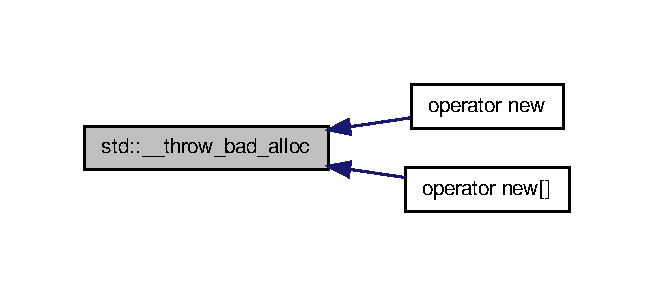
\includegraphics[width=314pt]{namespacestd_abddd698d3c2c32512f6d480fb0f1af46_icgraph}
\end{center}
\end{figure}


\hypertarget{namespacestd_a2d4fa0d6d5159bf0ab405e554327ac3b}{\index{std@{std}!\-\_\-\-\_\-throw\-\_\-invalid\-\_\-argument@{\-\_\-\-\_\-throw\-\_\-invalid\-\_\-argument}}
\index{\-\_\-\-\_\-throw\-\_\-invalid\-\_\-argument@{\-\_\-\-\_\-throw\-\_\-invalid\-\_\-argument}!std@{std}}
\subsubsection[{\-\_\-\-\_\-throw\-\_\-invalid\-\_\-argument}]{\setlength{\rightskip}{0pt plus 5cm}\-\_\-\-U\-C\-X\-X\-E\-X\-P\-O\-R\-T void std\-::\-\_\-\-\_\-throw\-\_\-invalid\-\_\-argument (
\begin{DoxyParamCaption}
\item[{const char $\ast$}]{}
\end{DoxyParamCaption}
)}}\label{namespacestd_a2d4fa0d6d5159bf0ab405e554327ac3b}
\hypertarget{namespacestd_a3d71257462d702a028190937e9425af1}{\index{std@{std}!\-\_\-\-\_\-throw\-\_\-length\-\_\-error@{\-\_\-\-\_\-throw\-\_\-length\-\_\-error}}
\index{\-\_\-\-\_\-throw\-\_\-length\-\_\-error@{\-\_\-\-\_\-throw\-\_\-length\-\_\-error}!std@{std}}
\subsubsection[{\-\_\-\-\_\-throw\-\_\-length\-\_\-error}]{\setlength{\rightskip}{0pt plus 5cm}\-\_\-\-U\-C\-X\-X\-E\-X\-P\-O\-R\-T void std\-::\-\_\-\-\_\-throw\-\_\-length\-\_\-error (
\begin{DoxyParamCaption}
\item[{const char $\ast$}]{}
\end{DoxyParamCaption}
)}}\label{namespacestd_a3d71257462d702a028190937e9425af1}
\hypertarget{namespacestd_a44237856ed577d4e70f4adc6a3f09a07}{\index{std@{std}!\-\_\-\-\_\-throw\-\_\-out\-\_\-of\-\_\-range@{\-\_\-\-\_\-throw\-\_\-out\-\_\-of\-\_\-range}}
\index{\-\_\-\-\_\-throw\-\_\-out\-\_\-of\-\_\-range@{\-\_\-\-\_\-throw\-\_\-out\-\_\-of\-\_\-range}!std@{std}}
\subsubsection[{\-\_\-\-\_\-throw\-\_\-out\-\_\-of\-\_\-range}]{\setlength{\rightskip}{0pt plus 5cm}\-\_\-\-U\-C\-X\-X\-E\-X\-P\-O\-R\-T void std\-::\-\_\-\-\_\-throw\-\_\-out\-\_\-of\-\_\-range (
\begin{DoxyParamCaption}
\item[{const char $\ast$}]{}
\end{DoxyParamCaption}
)}}\label{namespacestd_a44237856ed577d4e70f4adc6a3f09a07}
\hypertarget{namespacestd_ae216c5fcab3d1e7bd9216682922b2c8a}{\index{std@{std}!\-\_\-\-\_\-throw\-\_\-overflow\-\_\-error@{\-\_\-\-\_\-throw\-\_\-overflow\-\_\-error}}
\index{\-\_\-\-\_\-throw\-\_\-overflow\-\_\-error@{\-\_\-\-\_\-throw\-\_\-overflow\-\_\-error}!std@{std}}
\subsubsection[{\-\_\-\-\_\-throw\-\_\-overflow\-\_\-error}]{\setlength{\rightskip}{0pt plus 5cm}\-\_\-\-U\-C\-X\-X\-E\-X\-P\-O\-R\-T void std\-::\-\_\-\-\_\-throw\-\_\-overflow\-\_\-error (
\begin{DoxyParamCaption}
\item[{const char $\ast$}]{}
\end{DoxyParamCaption}
)}}\label{namespacestd_ae216c5fcab3d1e7bd9216682922b2c8a}


\subsection{Variable Documentation}
\hypertarget{namespacestd_abc249af4dfaee52181a0d6d241817c9e}{\index{std@{std}!complex$<$ float $>$@{complex$<$ float $>$}}
\index{complex$<$ float $>$@{complex$<$ float $>$}!std@{std}}
\subsubsection[{complex$<$ float $>$}]{\setlength{\rightskip}{0pt plus 5cm}template class \-\_\-\-U\-C\-X\-X\-E\-X\-P\-O\-R\-T std\-::complex$<$ float $>$}}\label{namespacestd_abc249af4dfaee52181a0d6d241817c9e}

\chapter{Class Documentation}
\hypertarget{struct____cxxabiv1_1_1____cxa__dependent__exception}{\section{\-\_\-\-\_\-cxxabiv1\-:\-:\-\_\-\-\_\-cxa\-\_\-dependent\-\_\-exception Struct Reference}
\label{struct____cxxabiv1_1_1____cxa__dependent__exception}\index{\-\_\-\-\_\-cxxabiv1\-::\-\_\-\-\_\-cxa\-\_\-dependent\-\_\-exception@{\-\_\-\-\_\-cxxabiv1\-::\-\_\-\-\_\-cxa\-\_\-dependent\-\_\-exception}}
}


{\ttfamily \#include $<$unwind-\/cxx.\-h$>$}



Collaboration diagram for \-\_\-\-\_\-cxxabiv1\-:\-:\-\_\-\-\_\-cxa\-\_\-dependent\-\_\-exception\-:\nopagebreak
\begin{figure}[H]
\begin{center}
\leavevmode
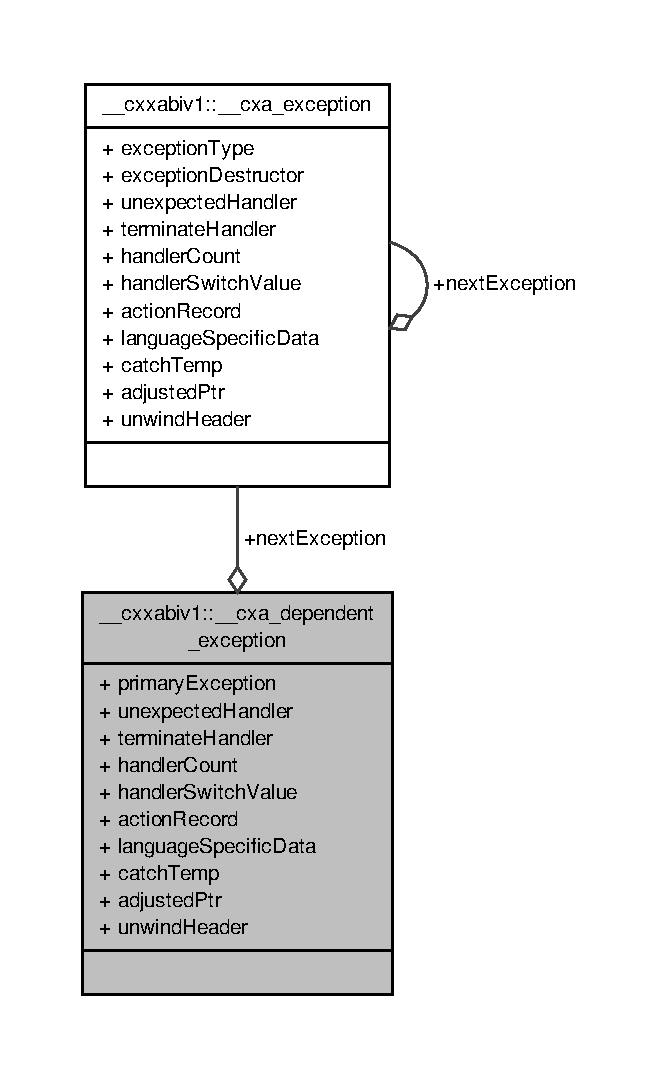
\includegraphics[width=317pt]{struct____cxxabiv1_1_1____cxa__dependent__exception__coll__graph}
\end{center}
\end{figure}
\subsection*{Public Attributes}
\begin{DoxyCompactItemize}
\item 
void $\ast$ \hyperlink{struct____cxxabiv1_1_1____cxa__dependent__exception_a30589654a3d486998f5e1453ec6cc53f}{primary\-Exception}
\item 
std\-::unexpected\-\_\-handler \hyperlink{struct____cxxabiv1_1_1____cxa__dependent__exception_a96024f9dca222992f78b43661f734879}{unexpected\-Handler}
\item 
std\-::terminate\-\_\-handler \hyperlink{struct____cxxabiv1_1_1____cxa__dependent__exception_a56317adb0bf2e865d1470eb73cc16b6c}{terminate\-Handler}
\item 
\hyperlink{struct____cxxabiv1_1_1____cxa__exception}{\-\_\-\-\_\-cxa\-\_\-exception} $\ast$ \hyperlink{struct____cxxabiv1_1_1____cxa__dependent__exception_a0866b87d824ae3da0268bef4be1fb206}{next\-Exception}
\item 
int \hyperlink{struct____cxxabiv1_1_1____cxa__dependent__exception_ab30402cb89b42f3a5f56586bb6c5573f}{handler\-Count}
\item 
int \hyperlink{struct____cxxabiv1_1_1____cxa__dependent__exception_a9dc794d946fabdceb7ed7b6949d2a1b0}{handler\-Switch\-Value}
\item 
const unsigned char $\ast$ \hyperlink{struct____cxxabiv1_1_1____cxa__dependent__exception_a46978a9c82858934d89abf7ff49de1d9}{action\-Record}
\item 
const unsigned char $\ast$ \hyperlink{struct____cxxabiv1_1_1____cxa__dependent__exception_acfbd8763036d11784a4785e21dff728b}{language\-Specific\-Data}
\item 
\-\_\-\-Unwind\-\_\-\-Ptr \hyperlink{struct____cxxabiv1_1_1____cxa__dependent__exception_ab6f374db0f84f5c988a89b0b9fdb663f}{catch\-Temp}
\item 
void $\ast$ \hyperlink{struct____cxxabiv1_1_1____cxa__dependent__exception_a4ab0524d6e60405ee733bc23363c8f5b}{adjusted\-Ptr}
\item 
\-\_\-\-Unwind\-\_\-\-Exception \hyperlink{struct____cxxabiv1_1_1____cxa__dependent__exception_af9053e3aad7c19d930d3ee225b31daad}{unwind\-Header}
\end{DoxyCompactItemize}


\subsection{Member Data Documentation}
\hypertarget{struct____cxxabiv1_1_1____cxa__dependent__exception_a46978a9c82858934d89abf7ff49de1d9}{\index{\-\_\-\-\_\-cxxabiv1\-::\-\_\-\-\_\-cxa\-\_\-dependent\-\_\-exception@{\-\_\-\-\_\-cxxabiv1\-::\-\_\-\-\_\-cxa\-\_\-dependent\-\_\-exception}!action\-Record@{action\-Record}}
\index{action\-Record@{action\-Record}!__cxxabiv1::__cxa_dependent_exception@{\-\_\-\-\_\-cxxabiv1\-::\-\_\-\-\_\-cxa\-\_\-dependent\-\_\-exception}}
\subsubsection[{action\-Record}]{\setlength{\rightskip}{0pt plus 5cm}const unsigned char$\ast$ \-\_\-\-\_\-cxxabiv1\-::\-\_\-\-\_\-cxa\-\_\-dependent\-\_\-exception\-::action\-Record}}\label{struct____cxxabiv1_1_1____cxa__dependent__exception_a46978a9c82858934d89abf7ff49de1d9}
\hypertarget{struct____cxxabiv1_1_1____cxa__dependent__exception_a4ab0524d6e60405ee733bc23363c8f5b}{\index{\-\_\-\-\_\-cxxabiv1\-::\-\_\-\-\_\-cxa\-\_\-dependent\-\_\-exception@{\-\_\-\-\_\-cxxabiv1\-::\-\_\-\-\_\-cxa\-\_\-dependent\-\_\-exception}!adjusted\-Ptr@{adjusted\-Ptr}}
\index{adjusted\-Ptr@{adjusted\-Ptr}!__cxxabiv1::__cxa_dependent_exception@{\-\_\-\-\_\-cxxabiv1\-::\-\_\-\-\_\-cxa\-\_\-dependent\-\_\-exception}}
\subsubsection[{adjusted\-Ptr}]{\setlength{\rightskip}{0pt plus 5cm}void$\ast$ \-\_\-\-\_\-cxxabiv1\-::\-\_\-\-\_\-cxa\-\_\-dependent\-\_\-exception\-::adjusted\-Ptr}}\label{struct____cxxabiv1_1_1____cxa__dependent__exception_a4ab0524d6e60405ee733bc23363c8f5b}
\hypertarget{struct____cxxabiv1_1_1____cxa__dependent__exception_ab6f374db0f84f5c988a89b0b9fdb663f}{\index{\-\_\-\-\_\-cxxabiv1\-::\-\_\-\-\_\-cxa\-\_\-dependent\-\_\-exception@{\-\_\-\-\_\-cxxabiv1\-::\-\_\-\-\_\-cxa\-\_\-dependent\-\_\-exception}!catch\-Temp@{catch\-Temp}}
\index{catch\-Temp@{catch\-Temp}!__cxxabiv1::__cxa_dependent_exception@{\-\_\-\-\_\-cxxabiv1\-::\-\_\-\-\_\-cxa\-\_\-dependent\-\_\-exception}}
\subsubsection[{catch\-Temp}]{\setlength{\rightskip}{0pt plus 5cm}\-\_\-\-Unwind\-\_\-\-Ptr \-\_\-\-\_\-cxxabiv1\-::\-\_\-\-\_\-cxa\-\_\-dependent\-\_\-exception\-::catch\-Temp}}\label{struct____cxxabiv1_1_1____cxa__dependent__exception_ab6f374db0f84f5c988a89b0b9fdb663f}
\hypertarget{struct____cxxabiv1_1_1____cxa__dependent__exception_ab30402cb89b42f3a5f56586bb6c5573f}{\index{\-\_\-\-\_\-cxxabiv1\-::\-\_\-\-\_\-cxa\-\_\-dependent\-\_\-exception@{\-\_\-\-\_\-cxxabiv1\-::\-\_\-\-\_\-cxa\-\_\-dependent\-\_\-exception}!handler\-Count@{handler\-Count}}
\index{handler\-Count@{handler\-Count}!__cxxabiv1::__cxa_dependent_exception@{\-\_\-\-\_\-cxxabiv1\-::\-\_\-\-\_\-cxa\-\_\-dependent\-\_\-exception}}
\subsubsection[{handler\-Count}]{\setlength{\rightskip}{0pt plus 5cm}int \-\_\-\-\_\-cxxabiv1\-::\-\_\-\-\_\-cxa\-\_\-dependent\-\_\-exception\-::handler\-Count}}\label{struct____cxxabiv1_1_1____cxa__dependent__exception_ab30402cb89b42f3a5f56586bb6c5573f}
\hypertarget{struct____cxxabiv1_1_1____cxa__dependent__exception_a9dc794d946fabdceb7ed7b6949d2a1b0}{\index{\-\_\-\-\_\-cxxabiv1\-::\-\_\-\-\_\-cxa\-\_\-dependent\-\_\-exception@{\-\_\-\-\_\-cxxabiv1\-::\-\_\-\-\_\-cxa\-\_\-dependent\-\_\-exception}!handler\-Switch\-Value@{handler\-Switch\-Value}}
\index{handler\-Switch\-Value@{handler\-Switch\-Value}!__cxxabiv1::__cxa_dependent_exception@{\-\_\-\-\_\-cxxabiv1\-::\-\_\-\-\_\-cxa\-\_\-dependent\-\_\-exception}}
\subsubsection[{handler\-Switch\-Value}]{\setlength{\rightskip}{0pt plus 5cm}int \-\_\-\-\_\-cxxabiv1\-::\-\_\-\-\_\-cxa\-\_\-dependent\-\_\-exception\-::handler\-Switch\-Value}}\label{struct____cxxabiv1_1_1____cxa__dependent__exception_a9dc794d946fabdceb7ed7b6949d2a1b0}
\hypertarget{struct____cxxabiv1_1_1____cxa__dependent__exception_acfbd8763036d11784a4785e21dff728b}{\index{\-\_\-\-\_\-cxxabiv1\-::\-\_\-\-\_\-cxa\-\_\-dependent\-\_\-exception@{\-\_\-\-\_\-cxxabiv1\-::\-\_\-\-\_\-cxa\-\_\-dependent\-\_\-exception}!language\-Specific\-Data@{language\-Specific\-Data}}
\index{language\-Specific\-Data@{language\-Specific\-Data}!__cxxabiv1::__cxa_dependent_exception@{\-\_\-\-\_\-cxxabiv1\-::\-\_\-\-\_\-cxa\-\_\-dependent\-\_\-exception}}
\subsubsection[{language\-Specific\-Data}]{\setlength{\rightskip}{0pt plus 5cm}const unsigned char$\ast$ \-\_\-\-\_\-cxxabiv1\-::\-\_\-\-\_\-cxa\-\_\-dependent\-\_\-exception\-::language\-Specific\-Data}}\label{struct____cxxabiv1_1_1____cxa__dependent__exception_acfbd8763036d11784a4785e21dff728b}
\hypertarget{struct____cxxabiv1_1_1____cxa__dependent__exception_a0866b87d824ae3da0268bef4be1fb206}{\index{\-\_\-\-\_\-cxxabiv1\-::\-\_\-\-\_\-cxa\-\_\-dependent\-\_\-exception@{\-\_\-\-\_\-cxxabiv1\-::\-\_\-\-\_\-cxa\-\_\-dependent\-\_\-exception}!next\-Exception@{next\-Exception}}
\index{next\-Exception@{next\-Exception}!__cxxabiv1::__cxa_dependent_exception@{\-\_\-\-\_\-cxxabiv1\-::\-\_\-\-\_\-cxa\-\_\-dependent\-\_\-exception}}
\subsubsection[{next\-Exception}]{\setlength{\rightskip}{0pt plus 5cm}{\bf \-\_\-\-\_\-cxa\-\_\-exception}$\ast$ \-\_\-\-\_\-cxxabiv1\-::\-\_\-\-\_\-cxa\-\_\-dependent\-\_\-exception\-::next\-Exception}}\label{struct____cxxabiv1_1_1____cxa__dependent__exception_a0866b87d824ae3da0268bef4be1fb206}
\hypertarget{struct____cxxabiv1_1_1____cxa__dependent__exception_a30589654a3d486998f5e1453ec6cc53f}{\index{\-\_\-\-\_\-cxxabiv1\-::\-\_\-\-\_\-cxa\-\_\-dependent\-\_\-exception@{\-\_\-\-\_\-cxxabiv1\-::\-\_\-\-\_\-cxa\-\_\-dependent\-\_\-exception}!primary\-Exception@{primary\-Exception}}
\index{primary\-Exception@{primary\-Exception}!__cxxabiv1::__cxa_dependent_exception@{\-\_\-\-\_\-cxxabiv1\-::\-\_\-\-\_\-cxa\-\_\-dependent\-\_\-exception}}
\subsubsection[{primary\-Exception}]{\setlength{\rightskip}{0pt plus 5cm}void$\ast$ \-\_\-\-\_\-cxxabiv1\-::\-\_\-\-\_\-cxa\-\_\-dependent\-\_\-exception\-::primary\-Exception}}\label{struct____cxxabiv1_1_1____cxa__dependent__exception_a30589654a3d486998f5e1453ec6cc53f}
\hypertarget{struct____cxxabiv1_1_1____cxa__dependent__exception_a56317adb0bf2e865d1470eb73cc16b6c}{\index{\-\_\-\-\_\-cxxabiv1\-::\-\_\-\-\_\-cxa\-\_\-dependent\-\_\-exception@{\-\_\-\-\_\-cxxabiv1\-::\-\_\-\-\_\-cxa\-\_\-dependent\-\_\-exception}!terminate\-Handler@{terminate\-Handler}}
\index{terminate\-Handler@{terminate\-Handler}!__cxxabiv1::__cxa_dependent_exception@{\-\_\-\-\_\-cxxabiv1\-::\-\_\-\-\_\-cxa\-\_\-dependent\-\_\-exception}}
\subsubsection[{terminate\-Handler}]{\setlength{\rightskip}{0pt plus 5cm}std\-::terminate\-\_\-handler \-\_\-\-\_\-cxxabiv1\-::\-\_\-\-\_\-cxa\-\_\-dependent\-\_\-exception\-::terminate\-Handler}}\label{struct____cxxabiv1_1_1____cxa__dependent__exception_a56317adb0bf2e865d1470eb73cc16b6c}
\hypertarget{struct____cxxabiv1_1_1____cxa__dependent__exception_a96024f9dca222992f78b43661f734879}{\index{\-\_\-\-\_\-cxxabiv1\-::\-\_\-\-\_\-cxa\-\_\-dependent\-\_\-exception@{\-\_\-\-\_\-cxxabiv1\-::\-\_\-\-\_\-cxa\-\_\-dependent\-\_\-exception}!unexpected\-Handler@{unexpected\-Handler}}
\index{unexpected\-Handler@{unexpected\-Handler}!__cxxabiv1::__cxa_dependent_exception@{\-\_\-\-\_\-cxxabiv1\-::\-\_\-\-\_\-cxa\-\_\-dependent\-\_\-exception}}
\subsubsection[{unexpected\-Handler}]{\setlength{\rightskip}{0pt plus 5cm}std\-::unexpected\-\_\-handler \-\_\-\-\_\-cxxabiv1\-::\-\_\-\-\_\-cxa\-\_\-dependent\-\_\-exception\-::unexpected\-Handler}}\label{struct____cxxabiv1_1_1____cxa__dependent__exception_a96024f9dca222992f78b43661f734879}
\hypertarget{struct____cxxabiv1_1_1____cxa__dependent__exception_af9053e3aad7c19d930d3ee225b31daad}{\index{\-\_\-\-\_\-cxxabiv1\-::\-\_\-\-\_\-cxa\-\_\-dependent\-\_\-exception@{\-\_\-\-\_\-cxxabiv1\-::\-\_\-\-\_\-cxa\-\_\-dependent\-\_\-exception}!unwind\-Header@{unwind\-Header}}
\index{unwind\-Header@{unwind\-Header}!__cxxabiv1::__cxa_dependent_exception@{\-\_\-\-\_\-cxxabiv1\-::\-\_\-\-\_\-cxa\-\_\-dependent\-\_\-exception}}
\subsubsection[{unwind\-Header}]{\setlength{\rightskip}{0pt plus 5cm}\-\_\-\-Unwind\-\_\-\-Exception \-\_\-\-\_\-cxxabiv1\-::\-\_\-\-\_\-cxa\-\_\-dependent\-\_\-exception\-::unwind\-Header}}\label{struct____cxxabiv1_1_1____cxa__dependent__exception_af9053e3aad7c19d930d3ee225b31daad}


The documentation for this struct was generated from the following file\-:\begin{DoxyCompactItemize}
\item 
lib/avr-\/stl/\hyperlink{unwind-cxx_8h}{unwind-\/cxx.\-h}\end{DoxyCompactItemize}

\hypertarget{struct____cxxabiv1_1_1____cxa__eh__globals}{\section{\-\_\-\-\_\-cxxabiv1\-:\-:\-\_\-\-\_\-cxa\-\_\-eh\-\_\-globals Struct Reference}
\label{struct____cxxabiv1_1_1____cxa__eh__globals}\index{\-\_\-\-\_\-cxxabiv1\-::\-\_\-\-\_\-cxa\-\_\-eh\-\_\-globals@{\-\_\-\-\_\-cxxabiv1\-::\-\_\-\-\_\-cxa\-\_\-eh\-\_\-globals}}
}


{\ttfamily \#include $<$unwind-\/cxx.\-h$>$}



Collaboration diagram for \-\_\-\-\_\-cxxabiv1\-:\-:\-\_\-\-\_\-cxa\-\_\-eh\-\_\-globals\-:\nopagebreak
\begin{figure}[H]
\begin{center}
\leavevmode
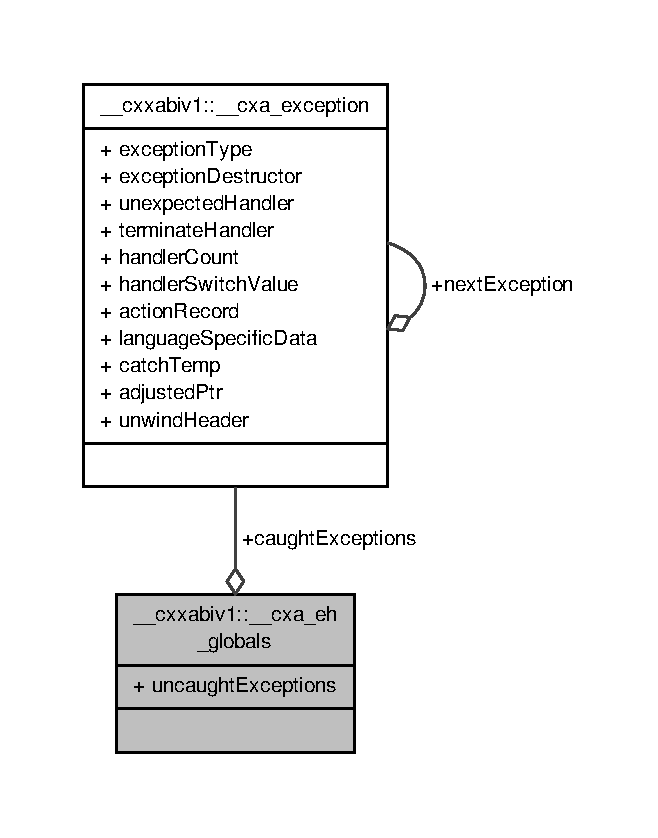
\includegraphics[width=316pt]{struct____cxxabiv1_1_1____cxa__eh__globals__coll__graph}
\end{center}
\end{figure}
\subsection*{Public Attributes}
\begin{DoxyCompactItemize}
\item 
\hyperlink{struct____cxxabiv1_1_1____cxa__exception}{\-\_\-\-\_\-cxa\-\_\-exception} $\ast$ \hyperlink{struct____cxxabiv1_1_1____cxa__eh__globals_a77348d2bb5877643cae07015a2453eb5}{caught\-Exceptions}
\item 
unsigned int \hyperlink{struct____cxxabiv1_1_1____cxa__eh__globals_a59d046223bdff74671ce9fc40d28bfa4}{uncaught\-Exceptions}
\end{DoxyCompactItemize}


\subsection{Member Data Documentation}
\hypertarget{struct____cxxabiv1_1_1____cxa__eh__globals_a77348d2bb5877643cae07015a2453eb5}{\index{\-\_\-\-\_\-cxxabiv1\-::\-\_\-\-\_\-cxa\-\_\-eh\-\_\-globals@{\-\_\-\-\_\-cxxabiv1\-::\-\_\-\-\_\-cxa\-\_\-eh\-\_\-globals}!caught\-Exceptions@{caught\-Exceptions}}
\index{caught\-Exceptions@{caught\-Exceptions}!__cxxabiv1::__cxa_eh_globals@{\-\_\-\-\_\-cxxabiv1\-::\-\_\-\-\_\-cxa\-\_\-eh\-\_\-globals}}
\subsubsection[{caught\-Exceptions}]{\setlength{\rightskip}{0pt plus 5cm}{\bf \-\_\-\-\_\-cxa\-\_\-exception}$\ast$ \-\_\-\-\_\-cxxabiv1\-::\-\_\-\-\_\-cxa\-\_\-eh\-\_\-globals\-::caught\-Exceptions}}\label{struct____cxxabiv1_1_1____cxa__eh__globals_a77348d2bb5877643cae07015a2453eb5}
\hypertarget{struct____cxxabiv1_1_1____cxa__eh__globals_a59d046223bdff74671ce9fc40d28bfa4}{\index{\-\_\-\-\_\-cxxabiv1\-::\-\_\-\-\_\-cxa\-\_\-eh\-\_\-globals@{\-\_\-\-\_\-cxxabiv1\-::\-\_\-\-\_\-cxa\-\_\-eh\-\_\-globals}!uncaught\-Exceptions@{uncaught\-Exceptions}}
\index{uncaught\-Exceptions@{uncaught\-Exceptions}!__cxxabiv1::__cxa_eh_globals@{\-\_\-\-\_\-cxxabiv1\-::\-\_\-\-\_\-cxa\-\_\-eh\-\_\-globals}}
\subsubsection[{uncaught\-Exceptions}]{\setlength{\rightskip}{0pt plus 5cm}unsigned int \-\_\-\-\_\-cxxabiv1\-::\-\_\-\-\_\-cxa\-\_\-eh\-\_\-globals\-::uncaught\-Exceptions}}\label{struct____cxxabiv1_1_1____cxa__eh__globals_a59d046223bdff74671ce9fc40d28bfa4}


The documentation for this struct was generated from the following file\-:\begin{DoxyCompactItemize}
\item 
lib/avr-\/stl/\hyperlink{unwind-cxx_8h}{unwind-\/cxx.\-h}\end{DoxyCompactItemize}

\hypertarget{struct____cxxabiv1_1_1____cxa__exception}{\section{\-\_\-\-\_\-cxxabiv1\-:\-:\-\_\-\-\_\-cxa\-\_\-exception Struct Reference}
\label{struct____cxxabiv1_1_1____cxa__exception}\index{\-\_\-\-\_\-cxxabiv1\-::\-\_\-\-\_\-cxa\-\_\-exception@{\-\_\-\-\_\-cxxabiv1\-::\-\_\-\-\_\-cxa\-\_\-exception}}
}


{\ttfamily \#include $<$unwind-\/cxx.\-h$>$}



Collaboration diagram for \-\_\-\-\_\-cxxabiv1\-:\-:\-\_\-\-\_\-cxa\-\_\-exception\-:\nopagebreak
\begin{figure}[H]
\begin{center}
\leavevmode
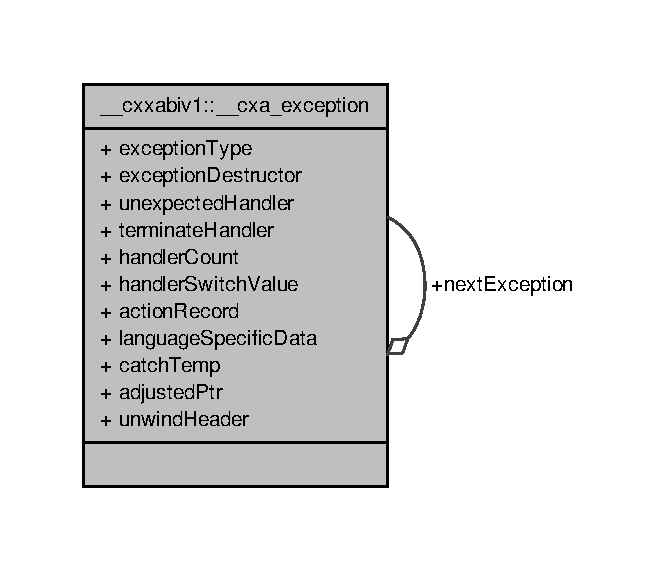
\includegraphics[width=316pt]{struct____cxxabiv1_1_1____cxa__exception__coll__graph}
\end{center}
\end{figure}
\subsection*{Public Attributes}
\begin{DoxyCompactItemize}
\item 
std\-::type\-\_\-info $\ast$ \hyperlink{struct____cxxabiv1_1_1____cxa__exception_ac64ad06829436c50fb5fb7c313e26866}{exception\-Type}
\item 
void($\ast$ \hyperlink{struct____cxxabiv1_1_1____cxa__exception_a1879a475548b2b52a017ed3007fd173d}{exception\-Destructor} )(void $\ast$)
\item 
std\-::unexpected\-\_\-handler \hyperlink{struct____cxxabiv1_1_1____cxa__exception_a54eaa8792b9d70a6fba263bc4098ccde}{unexpected\-Handler}
\item 
std\-::terminate\-\_\-handler \hyperlink{struct____cxxabiv1_1_1____cxa__exception_a95e8ed26809a82a5b1d404742665f12c}{terminate\-Handler}
\item 
\hyperlink{struct____cxxabiv1_1_1____cxa__exception}{\-\_\-\-\_\-cxa\-\_\-exception} $\ast$ \hyperlink{struct____cxxabiv1_1_1____cxa__exception_a8e5735018d1716ce01ad2da8ee8b6cd3}{next\-Exception}
\item 
int \hyperlink{struct____cxxabiv1_1_1____cxa__exception_a8fd8db34da0b3179081bfd6959a5a80a}{handler\-Count}
\item 
int \hyperlink{struct____cxxabiv1_1_1____cxa__exception_a98f471d3a99012797f9037e217aee520}{handler\-Switch\-Value}
\item 
const unsigned char $\ast$ \hyperlink{struct____cxxabiv1_1_1____cxa__exception_a5f946776edf58b5b8c3566b5f408d811}{action\-Record}
\item 
const unsigned char $\ast$ \hyperlink{struct____cxxabiv1_1_1____cxa__exception_a57fea26051378a6a5f5c239f5b86b06f}{language\-Specific\-Data}
\item 
\-\_\-\-Unwind\-\_\-\-Ptr \hyperlink{struct____cxxabiv1_1_1____cxa__exception_ad27f857d1fe7e865672e96fc2549955d}{catch\-Temp}
\item 
void $\ast$ \hyperlink{struct____cxxabiv1_1_1____cxa__exception_a8bbedb8ce8835dd97247dce153ccf281}{adjusted\-Ptr}
\item 
\-\_\-\-Unwind\-\_\-\-Exception \hyperlink{struct____cxxabiv1_1_1____cxa__exception_af6f09c0335f5982eb75942fc2c2abdd4}{unwind\-Header}
\end{DoxyCompactItemize}


\subsection{Member Data Documentation}
\hypertarget{struct____cxxabiv1_1_1____cxa__exception_a5f946776edf58b5b8c3566b5f408d811}{\index{\-\_\-\-\_\-cxxabiv1\-::\-\_\-\-\_\-cxa\-\_\-exception@{\-\_\-\-\_\-cxxabiv1\-::\-\_\-\-\_\-cxa\-\_\-exception}!action\-Record@{action\-Record}}
\index{action\-Record@{action\-Record}!__cxxabiv1::__cxa_exception@{\-\_\-\-\_\-cxxabiv1\-::\-\_\-\-\_\-cxa\-\_\-exception}}
\subsubsection[{action\-Record}]{\setlength{\rightskip}{0pt plus 5cm}const unsigned char$\ast$ \-\_\-\-\_\-cxxabiv1\-::\-\_\-\-\_\-cxa\-\_\-exception\-::action\-Record}}\label{struct____cxxabiv1_1_1____cxa__exception_a5f946776edf58b5b8c3566b5f408d811}
\hypertarget{struct____cxxabiv1_1_1____cxa__exception_a8bbedb8ce8835dd97247dce153ccf281}{\index{\-\_\-\-\_\-cxxabiv1\-::\-\_\-\-\_\-cxa\-\_\-exception@{\-\_\-\-\_\-cxxabiv1\-::\-\_\-\-\_\-cxa\-\_\-exception}!adjusted\-Ptr@{adjusted\-Ptr}}
\index{adjusted\-Ptr@{adjusted\-Ptr}!__cxxabiv1::__cxa_exception@{\-\_\-\-\_\-cxxabiv1\-::\-\_\-\-\_\-cxa\-\_\-exception}}
\subsubsection[{adjusted\-Ptr}]{\setlength{\rightskip}{0pt plus 5cm}void$\ast$ \-\_\-\-\_\-cxxabiv1\-::\-\_\-\-\_\-cxa\-\_\-exception\-::adjusted\-Ptr}}\label{struct____cxxabiv1_1_1____cxa__exception_a8bbedb8ce8835dd97247dce153ccf281}
\hypertarget{struct____cxxabiv1_1_1____cxa__exception_ad27f857d1fe7e865672e96fc2549955d}{\index{\-\_\-\-\_\-cxxabiv1\-::\-\_\-\-\_\-cxa\-\_\-exception@{\-\_\-\-\_\-cxxabiv1\-::\-\_\-\-\_\-cxa\-\_\-exception}!catch\-Temp@{catch\-Temp}}
\index{catch\-Temp@{catch\-Temp}!__cxxabiv1::__cxa_exception@{\-\_\-\-\_\-cxxabiv1\-::\-\_\-\-\_\-cxa\-\_\-exception}}
\subsubsection[{catch\-Temp}]{\setlength{\rightskip}{0pt plus 5cm}\-\_\-\-Unwind\-\_\-\-Ptr \-\_\-\-\_\-cxxabiv1\-::\-\_\-\-\_\-cxa\-\_\-exception\-::catch\-Temp}}\label{struct____cxxabiv1_1_1____cxa__exception_ad27f857d1fe7e865672e96fc2549955d}
\hypertarget{struct____cxxabiv1_1_1____cxa__exception_a1879a475548b2b52a017ed3007fd173d}{\index{\-\_\-\-\_\-cxxabiv1\-::\-\_\-\-\_\-cxa\-\_\-exception@{\-\_\-\-\_\-cxxabiv1\-::\-\_\-\-\_\-cxa\-\_\-exception}!exception\-Destructor@{exception\-Destructor}}
\index{exception\-Destructor@{exception\-Destructor}!__cxxabiv1::__cxa_exception@{\-\_\-\-\_\-cxxabiv1\-::\-\_\-\-\_\-cxa\-\_\-exception}}
\subsubsection[{exception\-Destructor}]{\setlength{\rightskip}{0pt plus 5cm}void($\ast$ \-\_\-\-\_\-cxxabiv1\-::\-\_\-\-\_\-cxa\-\_\-exception\-::exception\-Destructor)(void $\ast$)}}\label{struct____cxxabiv1_1_1____cxa__exception_a1879a475548b2b52a017ed3007fd173d}
\hypertarget{struct____cxxabiv1_1_1____cxa__exception_ac64ad06829436c50fb5fb7c313e26866}{\index{\-\_\-\-\_\-cxxabiv1\-::\-\_\-\-\_\-cxa\-\_\-exception@{\-\_\-\-\_\-cxxabiv1\-::\-\_\-\-\_\-cxa\-\_\-exception}!exception\-Type@{exception\-Type}}
\index{exception\-Type@{exception\-Type}!__cxxabiv1::__cxa_exception@{\-\_\-\-\_\-cxxabiv1\-::\-\_\-\-\_\-cxa\-\_\-exception}}
\subsubsection[{exception\-Type}]{\setlength{\rightskip}{0pt plus 5cm}std\-::type\-\_\-info$\ast$ \-\_\-\-\_\-cxxabiv1\-::\-\_\-\-\_\-cxa\-\_\-exception\-::exception\-Type}}\label{struct____cxxabiv1_1_1____cxa__exception_ac64ad06829436c50fb5fb7c313e26866}
\hypertarget{struct____cxxabiv1_1_1____cxa__exception_a8fd8db34da0b3179081bfd6959a5a80a}{\index{\-\_\-\-\_\-cxxabiv1\-::\-\_\-\-\_\-cxa\-\_\-exception@{\-\_\-\-\_\-cxxabiv1\-::\-\_\-\-\_\-cxa\-\_\-exception}!handler\-Count@{handler\-Count}}
\index{handler\-Count@{handler\-Count}!__cxxabiv1::__cxa_exception@{\-\_\-\-\_\-cxxabiv1\-::\-\_\-\-\_\-cxa\-\_\-exception}}
\subsubsection[{handler\-Count}]{\setlength{\rightskip}{0pt plus 5cm}int \-\_\-\-\_\-cxxabiv1\-::\-\_\-\-\_\-cxa\-\_\-exception\-::handler\-Count}}\label{struct____cxxabiv1_1_1____cxa__exception_a8fd8db34da0b3179081bfd6959a5a80a}
\hypertarget{struct____cxxabiv1_1_1____cxa__exception_a98f471d3a99012797f9037e217aee520}{\index{\-\_\-\-\_\-cxxabiv1\-::\-\_\-\-\_\-cxa\-\_\-exception@{\-\_\-\-\_\-cxxabiv1\-::\-\_\-\-\_\-cxa\-\_\-exception}!handler\-Switch\-Value@{handler\-Switch\-Value}}
\index{handler\-Switch\-Value@{handler\-Switch\-Value}!__cxxabiv1::__cxa_exception@{\-\_\-\-\_\-cxxabiv1\-::\-\_\-\-\_\-cxa\-\_\-exception}}
\subsubsection[{handler\-Switch\-Value}]{\setlength{\rightskip}{0pt plus 5cm}int \-\_\-\-\_\-cxxabiv1\-::\-\_\-\-\_\-cxa\-\_\-exception\-::handler\-Switch\-Value}}\label{struct____cxxabiv1_1_1____cxa__exception_a98f471d3a99012797f9037e217aee520}
\hypertarget{struct____cxxabiv1_1_1____cxa__exception_a57fea26051378a6a5f5c239f5b86b06f}{\index{\-\_\-\-\_\-cxxabiv1\-::\-\_\-\-\_\-cxa\-\_\-exception@{\-\_\-\-\_\-cxxabiv1\-::\-\_\-\-\_\-cxa\-\_\-exception}!language\-Specific\-Data@{language\-Specific\-Data}}
\index{language\-Specific\-Data@{language\-Specific\-Data}!__cxxabiv1::__cxa_exception@{\-\_\-\-\_\-cxxabiv1\-::\-\_\-\-\_\-cxa\-\_\-exception}}
\subsubsection[{language\-Specific\-Data}]{\setlength{\rightskip}{0pt plus 5cm}const unsigned char$\ast$ \-\_\-\-\_\-cxxabiv1\-::\-\_\-\-\_\-cxa\-\_\-exception\-::language\-Specific\-Data}}\label{struct____cxxabiv1_1_1____cxa__exception_a57fea26051378a6a5f5c239f5b86b06f}
\hypertarget{struct____cxxabiv1_1_1____cxa__exception_a8e5735018d1716ce01ad2da8ee8b6cd3}{\index{\-\_\-\-\_\-cxxabiv1\-::\-\_\-\-\_\-cxa\-\_\-exception@{\-\_\-\-\_\-cxxabiv1\-::\-\_\-\-\_\-cxa\-\_\-exception}!next\-Exception@{next\-Exception}}
\index{next\-Exception@{next\-Exception}!__cxxabiv1::__cxa_exception@{\-\_\-\-\_\-cxxabiv1\-::\-\_\-\-\_\-cxa\-\_\-exception}}
\subsubsection[{next\-Exception}]{\setlength{\rightskip}{0pt plus 5cm}{\bf \-\_\-\-\_\-cxa\-\_\-exception}$\ast$ \-\_\-\-\_\-cxxabiv1\-::\-\_\-\-\_\-cxa\-\_\-exception\-::next\-Exception}}\label{struct____cxxabiv1_1_1____cxa__exception_a8e5735018d1716ce01ad2da8ee8b6cd3}
\hypertarget{struct____cxxabiv1_1_1____cxa__exception_a95e8ed26809a82a5b1d404742665f12c}{\index{\-\_\-\-\_\-cxxabiv1\-::\-\_\-\-\_\-cxa\-\_\-exception@{\-\_\-\-\_\-cxxabiv1\-::\-\_\-\-\_\-cxa\-\_\-exception}!terminate\-Handler@{terminate\-Handler}}
\index{terminate\-Handler@{terminate\-Handler}!__cxxabiv1::__cxa_exception@{\-\_\-\-\_\-cxxabiv1\-::\-\_\-\-\_\-cxa\-\_\-exception}}
\subsubsection[{terminate\-Handler}]{\setlength{\rightskip}{0pt plus 5cm}std\-::terminate\-\_\-handler \-\_\-\-\_\-cxxabiv1\-::\-\_\-\-\_\-cxa\-\_\-exception\-::terminate\-Handler}}\label{struct____cxxabiv1_1_1____cxa__exception_a95e8ed26809a82a5b1d404742665f12c}
\hypertarget{struct____cxxabiv1_1_1____cxa__exception_a54eaa8792b9d70a6fba263bc4098ccde}{\index{\-\_\-\-\_\-cxxabiv1\-::\-\_\-\-\_\-cxa\-\_\-exception@{\-\_\-\-\_\-cxxabiv1\-::\-\_\-\-\_\-cxa\-\_\-exception}!unexpected\-Handler@{unexpected\-Handler}}
\index{unexpected\-Handler@{unexpected\-Handler}!__cxxabiv1::__cxa_exception@{\-\_\-\-\_\-cxxabiv1\-::\-\_\-\-\_\-cxa\-\_\-exception}}
\subsubsection[{unexpected\-Handler}]{\setlength{\rightskip}{0pt plus 5cm}std\-::unexpected\-\_\-handler \-\_\-\-\_\-cxxabiv1\-::\-\_\-\-\_\-cxa\-\_\-exception\-::unexpected\-Handler}}\label{struct____cxxabiv1_1_1____cxa__exception_a54eaa8792b9d70a6fba263bc4098ccde}
\hypertarget{struct____cxxabiv1_1_1____cxa__exception_af6f09c0335f5982eb75942fc2c2abdd4}{\index{\-\_\-\-\_\-cxxabiv1\-::\-\_\-\-\_\-cxa\-\_\-exception@{\-\_\-\-\_\-cxxabiv1\-::\-\_\-\-\_\-cxa\-\_\-exception}!unwind\-Header@{unwind\-Header}}
\index{unwind\-Header@{unwind\-Header}!__cxxabiv1::__cxa_exception@{\-\_\-\-\_\-cxxabiv1\-::\-\_\-\-\_\-cxa\-\_\-exception}}
\subsubsection[{unwind\-Header}]{\setlength{\rightskip}{0pt plus 5cm}\-\_\-\-Unwind\-\_\-\-Exception \-\_\-\-\_\-cxxabiv1\-::\-\_\-\-\_\-cxa\-\_\-exception\-::unwind\-Header}}\label{struct____cxxabiv1_1_1____cxa__exception_af6f09c0335f5982eb75942fc2c2abdd4}


The documentation for this struct was generated from the following file\-:\begin{DoxyCompactItemize}
\item 
lib/avr-\/stl/\hyperlink{unwind-cxx_8h}{unwind-\/cxx.\-h}\end{DoxyCompactItemize}

\hypertarget{struct_arduino}{\section{Arduino Struct Reference}
\label{struct_arduino}\index{Arduino@{Arduino}}
}


{\ttfamily \#include $<$Mock\-W\-Program.\-hpp$>$}



Collaboration diagram for Arduino\-:\nopagebreak
\begin{figure}[H]
\begin{center}
\leavevmode
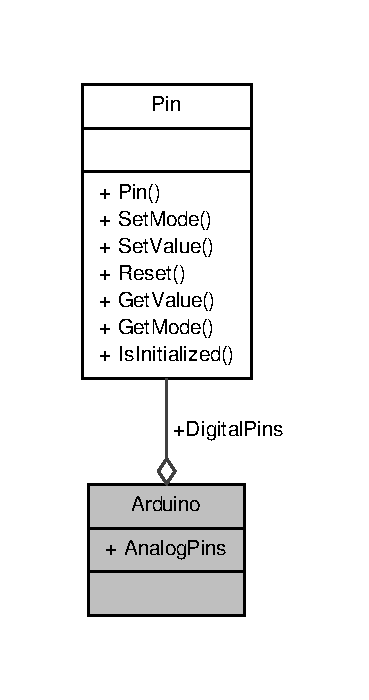
\includegraphics[width=177pt]{struct_arduino__coll__graph}
\end{center}
\end{figure}
\subsection*{Public Attributes}
\begin{DoxyCompactItemize}
\item 
\hyperlink{class_pin}{Pin} \hyperlink{struct_arduino_ae607ad57ed2b574c1db0e298d1700154}{Digital\-Pins} \mbox{[}14\mbox{]}
\item 
float \hyperlink{struct_arduino_a344478f98fe14a78faa30bb694d7b28d}{Analog\-Pins} \mbox{[}6\mbox{]}
\end{DoxyCompactItemize}


\subsection{Member Data Documentation}
\hypertarget{struct_arduino_a344478f98fe14a78faa30bb694d7b28d}{\index{Arduino@{Arduino}!Analog\-Pins@{Analog\-Pins}}
\index{Analog\-Pins@{Analog\-Pins}!Arduino@{Arduino}}
\subsubsection[{Analog\-Pins}]{\setlength{\rightskip}{0pt plus 5cm}float Arduino\-::\-Analog\-Pins\mbox{[}6\mbox{]}}}\label{struct_arduino_a344478f98fe14a78faa30bb694d7b28d}
\hypertarget{struct_arduino_ae607ad57ed2b574c1db0e298d1700154}{\index{Arduino@{Arduino}!Digital\-Pins@{Digital\-Pins}}
\index{Digital\-Pins@{Digital\-Pins}!Arduino@{Arduino}}
\subsubsection[{Digital\-Pins}]{\setlength{\rightskip}{0pt plus 5cm}{\bf Pin} Arduino\-::\-Digital\-Pins\mbox{[}14\mbox{]}}}\label{struct_arduino_ae607ad57ed2b574c1db0e298d1700154}


The documentation for this struct was generated from the following file\-:\begin{DoxyCompactItemize}
\item 
lib/arduino\-\_\-mocks/\hyperlink{_mock_w_program_8hpp}{Mock\-W\-Program.\-hpp}\end{DoxyCompactItemize}

\hypertarget{struct_arduino_setup}{\section{Arduino\-Setup Struct Reference}
\label{struct_arduino_setup}\index{Arduino\-Setup@{Arduino\-Setup}}
}


Collaboration diagram for Arduino\-Setup\-:\nopagebreak
\begin{figure}[H]
\begin{center}
\leavevmode
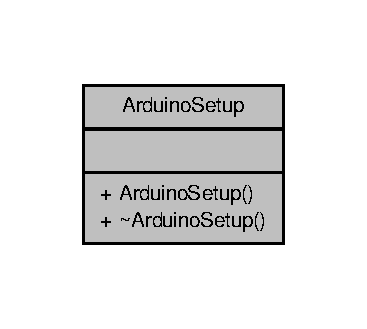
\includegraphics[width=176pt]{struct_arduino_setup__coll__graph}
\end{center}
\end{figure}
\subsection*{Public Member Functions}
\begin{DoxyCompactItemize}
\item 
\hyperlink{struct_arduino_setup_a4f042a0574fc29c3e6800d77db394b26}{Arduino\-Setup} ()
\item 
\hyperlink{struct_arduino_setup_ae5f1cafc910b2fa73692adaeed874e7a}{$\sim$\-Arduino\-Setup} ()
\end{DoxyCompactItemize}


\subsection{Constructor \& Destructor Documentation}
\hypertarget{struct_arduino_setup_a4f042a0574fc29c3e6800d77db394b26}{\index{Arduino\-Setup@{Arduino\-Setup}!Arduino\-Setup@{Arduino\-Setup}}
\index{Arduino\-Setup@{Arduino\-Setup}!ArduinoSetup@{Arduino\-Setup}}
\subsubsection[{Arduino\-Setup}]{\setlength{\rightskip}{0pt plus 5cm}Arduino\-Setup\-::\-Arduino\-Setup (
\begin{DoxyParamCaption}
{}
\end{DoxyParamCaption}
)\hspace{0.3cm}{\ttfamily [inline]}}}\label{struct_arduino_setup_a4f042a0574fc29c3e6800d77db394b26}


Here is the call graph for this function\-:\nopagebreak
\begin{figure}[H]
\begin{center}
\leavevmode
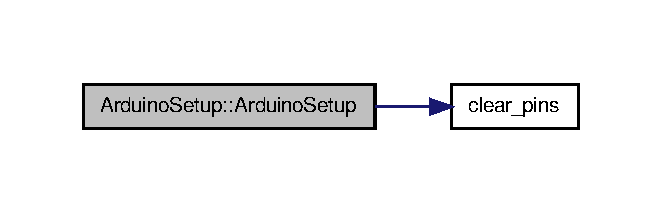
\includegraphics[width=318pt]{struct_arduino_setup_a4f042a0574fc29c3e6800d77db394b26_cgraph}
\end{center}
\end{figure}


\hypertarget{struct_arduino_setup_ae5f1cafc910b2fa73692adaeed874e7a}{\index{Arduino\-Setup@{Arduino\-Setup}!$\sim$\-Arduino\-Setup@{$\sim$\-Arduino\-Setup}}
\index{$\sim$\-Arduino\-Setup@{$\sim$\-Arduino\-Setup}!ArduinoSetup@{Arduino\-Setup}}
\subsubsection[{$\sim$\-Arduino\-Setup}]{\setlength{\rightskip}{0pt plus 5cm}Arduino\-Setup\-::$\sim$\-Arduino\-Setup (
\begin{DoxyParamCaption}
{}
\end{DoxyParamCaption}
)\hspace{0.3cm}{\ttfamily [inline]}}}\label{struct_arduino_setup_ae5f1cafc910b2fa73692adaeed874e7a}


Here is the call graph for this function\-:\nopagebreak
\begin{figure}[H]
\begin{center}
\leavevmode
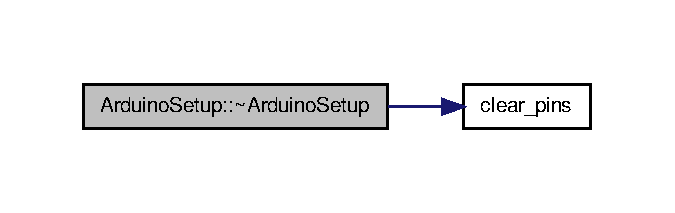
\includegraphics[width=324pt]{struct_arduino_setup_ae5f1cafc910b2fa73692adaeed874e7a_cgraph}
\end{center}
\end{figure}




The documentation for this struct was generated from the following file\-:\begin{DoxyCompactItemize}
\item 
lib/motor\-\_\-control/test/\hyperlink{_test_motor_8cpp}{Test\-Motor.\-cpp}\end{DoxyCompactItemize}

\hypertarget{class_encoder}{\section{Encoder Class Reference}
\label{class_encoder}\index{Encoder@{Encoder}}
}


{\ttfamily \#include $<$Encoder.\-h$>$}



Inheritance diagram for Encoder\-:
\nopagebreak
\begin{figure}[H]
\begin{center}
\leavevmode
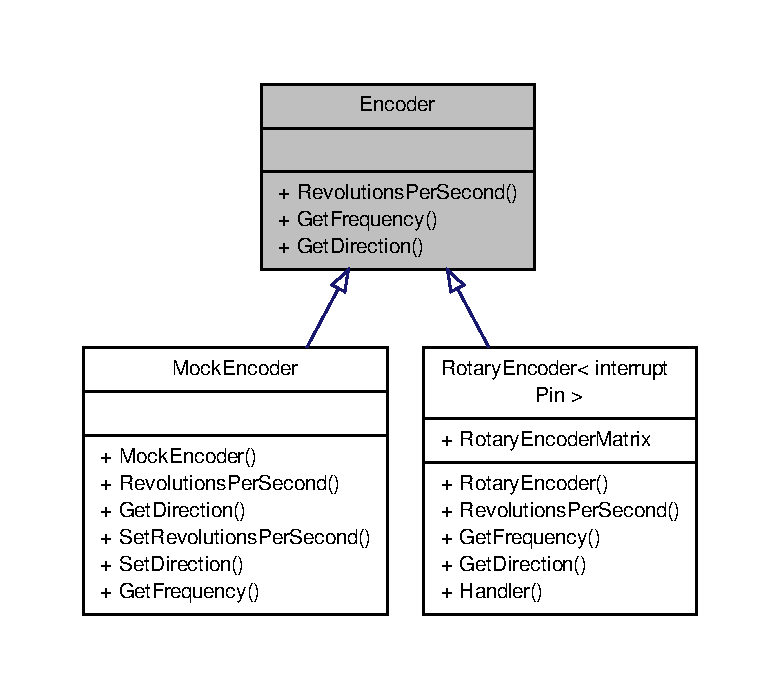
\includegraphics[width=350pt]{class_encoder__inherit__graph}
\end{center}
\end{figure}


Collaboration diagram for Encoder\-:
\nopagebreak
\begin{figure}[H]
\begin{center}
\leavevmode
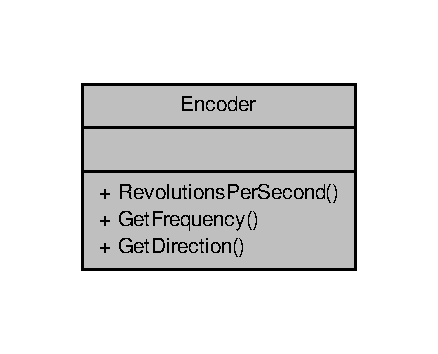
\includegraphics[width=210pt]{class_encoder__coll__graph}
\end{center}
\end{figure}
\subsection*{Public Types}
\begin{DoxyCompactItemize}
\item 
enum \hyperlink{class_encoder_aa7c4648a7ebc9e651c25c2d450a58213}{Direction} \{ \hyperlink{class_encoder_aa7c4648a7ebc9e651c25c2d450a58213a75ee06096317d25b47119647e33622cf}{F\-O\-R\-W\-A\-R\-D\-S} = 1, 
\hyperlink{class_encoder_aa7c4648a7ebc9e651c25c2d450a58213a9fb277421175dd4894688e30dd757253}{B\-A\-C\-K\-W\-A\-R\-D\-S} = -\/1
 \}
\end{DoxyCompactItemize}
\subsection*{Public Member Functions}
\begin{DoxyCompactItemize}
\item 
virtual float \hyperlink{class_encoder_a758adfad11078f8dec0ca672929a4189}{Revolutions\-Per\-Second} ()=0
\item 
virtual float \hyperlink{class_encoder_ab52587693b386731fcdef289e590fc40}{Get\-Frequency} ()=0
\item 
virtual \hyperlink{class_encoder_aa7c4648a7ebc9e651c25c2d450a58213}{Direction} \hyperlink{class_encoder_ab4faff630f313bc0e5b8718df3175fe1}{Get\-Direction} () const =0
\end{DoxyCompactItemize}


\subsection{Member Enumeration Documentation}
\hypertarget{class_encoder_aa7c4648a7ebc9e651c25c2d450a58213}{\index{Encoder@{Encoder}!Direction@{Direction}}
\index{Direction@{Direction}!Encoder@{Encoder}}
\subsubsection[{Direction}]{\setlength{\rightskip}{0pt plus 5cm}enum {\bf Encoder\-::\-Direction}}}\label{class_encoder_aa7c4648a7ebc9e651c25c2d450a58213}
\begin{Desc}
\item[Enumerator]\par
\begin{description}
\index{F\-O\-R\-W\-A\-R\-D\-S@{F\-O\-R\-W\-A\-R\-D\-S}!Encoder@{Encoder}}\index{Encoder@{Encoder}!F\-O\-R\-W\-A\-R\-D\-S@{F\-O\-R\-W\-A\-R\-D\-S}}\item[{\em 
\hypertarget{class_encoder_aa7c4648a7ebc9e651c25c2d450a58213a75ee06096317d25b47119647e33622cf}{F\-O\-R\-W\-A\-R\-D\-S}\label{class_encoder_aa7c4648a7ebc9e651c25c2d450a58213a75ee06096317d25b47119647e33622cf}
}]\index{B\-A\-C\-K\-W\-A\-R\-D\-S@{B\-A\-C\-K\-W\-A\-R\-D\-S}!Encoder@{Encoder}}\index{Encoder@{Encoder}!B\-A\-C\-K\-W\-A\-R\-D\-S@{B\-A\-C\-K\-W\-A\-R\-D\-S}}\item[{\em 
\hypertarget{class_encoder_aa7c4648a7ebc9e651c25c2d450a58213a9fb277421175dd4894688e30dd757253}{B\-A\-C\-K\-W\-A\-R\-D\-S}\label{class_encoder_aa7c4648a7ebc9e651c25c2d450a58213a9fb277421175dd4894688e30dd757253}
}]\end{description}
\end{Desc}


\subsection{Member Function Documentation}
\hypertarget{class_encoder_ab4faff630f313bc0e5b8718df3175fe1}{\index{Encoder@{Encoder}!Get\-Direction@{Get\-Direction}}
\index{Get\-Direction@{Get\-Direction}!Encoder@{Encoder}}
\subsubsection[{Get\-Direction}]{\setlength{\rightskip}{0pt plus 5cm}virtual {\bf Direction} Encoder\-::\-Get\-Direction (
\begin{DoxyParamCaption}
{}
\end{DoxyParamCaption}
) const\hspace{0.3cm}{\ttfamily [pure virtual]}}}\label{class_encoder_ab4faff630f313bc0e5b8718df3175fe1}


Implemented in \hyperlink{class_rotary_encoder_aa62141a77e01d0d44706f3b421e3ae25}{Rotary\-Encoder$<$ interrupt\-Pin $>$}, and \hyperlink{class_mock_encoder_a167ec4aad9f3f00217c25cec301f26b3}{Mock\-Encoder}.



Here is the caller graph for this function\-:\nopagebreak
\begin{figure}[H]
\begin{center}
\leavevmode
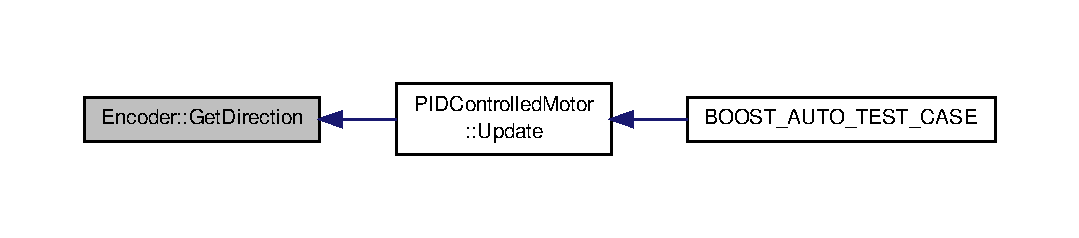
\includegraphics[width=350pt]{class_encoder_ab4faff630f313bc0e5b8718df3175fe1_icgraph}
\end{center}
\end{figure}


\hypertarget{class_encoder_ab52587693b386731fcdef289e590fc40}{\index{Encoder@{Encoder}!Get\-Frequency@{Get\-Frequency}}
\index{Get\-Frequency@{Get\-Frequency}!Encoder@{Encoder}}
\subsubsection[{Get\-Frequency}]{\setlength{\rightskip}{0pt plus 5cm}virtual float Encoder\-::\-Get\-Frequency (
\begin{DoxyParamCaption}
{}
\end{DoxyParamCaption}
)\hspace{0.3cm}{\ttfamily [pure virtual]}}}\label{class_encoder_ab52587693b386731fcdef289e590fc40}


Implemented in \hyperlink{class_rotary_encoder_a3dea9166b76dad99ee708c4ff1fde9f8}{Rotary\-Encoder$<$ interrupt\-Pin $>$}, and \hyperlink{class_mock_encoder_a586614c42fbf173f3809dea3e1b9c126}{Mock\-Encoder}.



Here is the caller graph for this function\-:\nopagebreak
\begin{figure}[H]
\begin{center}
\leavevmode
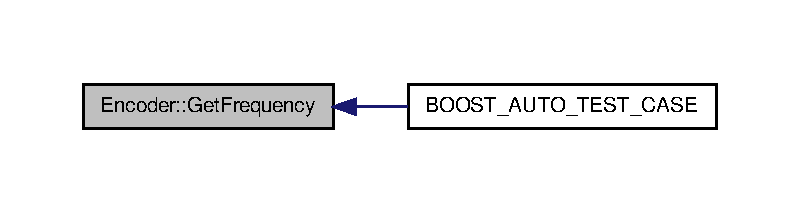
\includegraphics[width=350pt]{class_encoder_ab52587693b386731fcdef289e590fc40_icgraph}
\end{center}
\end{figure}


\hypertarget{class_encoder_a758adfad11078f8dec0ca672929a4189}{\index{Encoder@{Encoder}!Revolutions\-Per\-Second@{Revolutions\-Per\-Second}}
\index{Revolutions\-Per\-Second@{Revolutions\-Per\-Second}!Encoder@{Encoder}}
\subsubsection[{Revolutions\-Per\-Second}]{\setlength{\rightskip}{0pt plus 5cm}virtual float Encoder\-::\-Revolutions\-Per\-Second (
\begin{DoxyParamCaption}
{}
\end{DoxyParamCaption}
)\hspace{0.3cm}{\ttfamily [pure virtual]}}}\label{class_encoder_a758adfad11078f8dec0ca672929a4189}


Implemented in \hyperlink{class_rotary_encoder_a7ec02990f0ffb7bb62a3a76f0fd64ade}{Rotary\-Encoder$<$ interrupt\-Pin $>$}, and \hyperlink{class_mock_encoder_ad44313dd4a038f09084f04c908fa9a00}{Mock\-Encoder}.



Here is the caller graph for this function\-:\nopagebreak
\begin{figure}[H]
\begin{center}
\leavevmode
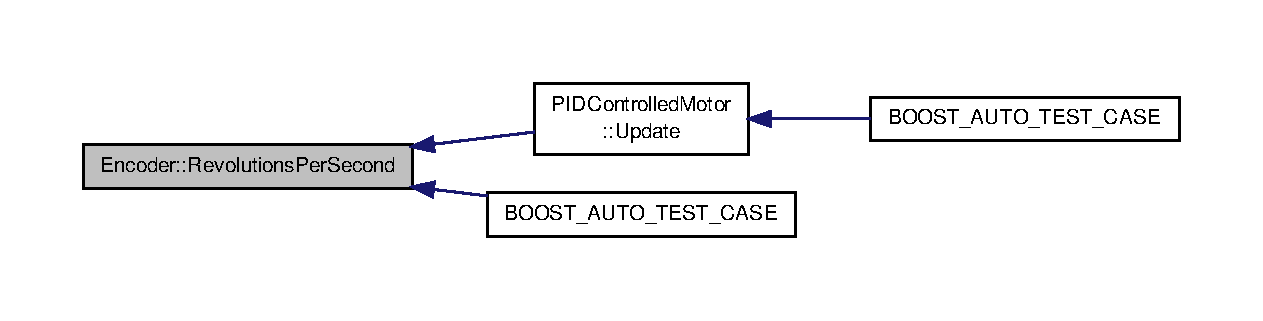
\includegraphics[width=350pt]{class_encoder_a758adfad11078f8dec0ca672929a4189_icgraph}
\end{center}
\end{figure}




The documentation for this class was generated from the following file\-:\begin{DoxyCompactItemize}
\item 
lib/odometry/\hyperlink{_encoder_8h}{Encoder.\-h}\end{DoxyCompactItemize}

\hypertarget{class_feedback_controlled_motor}{\section{Feedback\-Controlled\-Motor Class Reference}
\label{class_feedback_controlled_motor}\index{Feedback\-Controlled\-Motor@{Feedback\-Controlled\-Motor}}
}


{\ttfamily \#include $<$Feedback\-Controlled\-Motor.\-h$>$}



Inheritance diagram for Feedback\-Controlled\-Motor\-:
\nopagebreak
\begin{figure}[H]
\begin{center}
\leavevmode
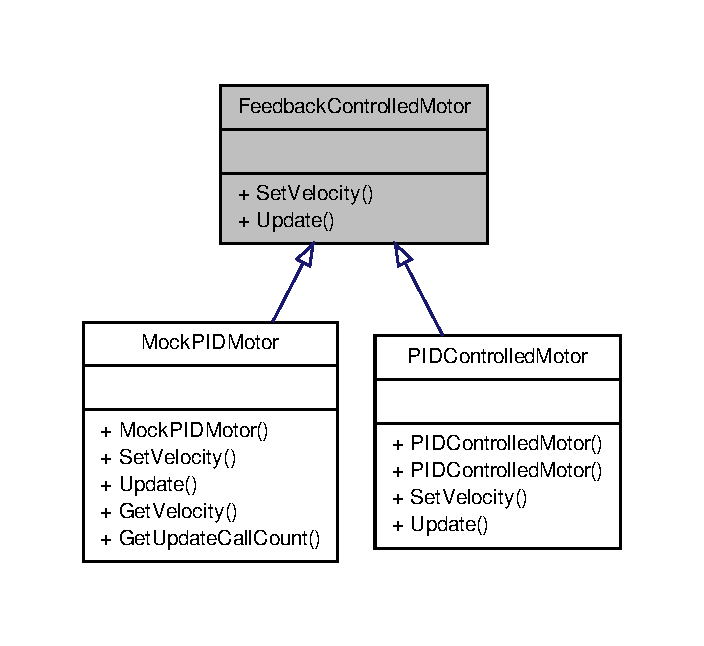
\includegraphics[width=338pt]{class_feedback_controlled_motor__inherit__graph}
\end{center}
\end{figure}


Collaboration diagram for Feedback\-Controlled\-Motor\-:
\nopagebreak
\begin{figure}[H]
\begin{center}
\leavevmode
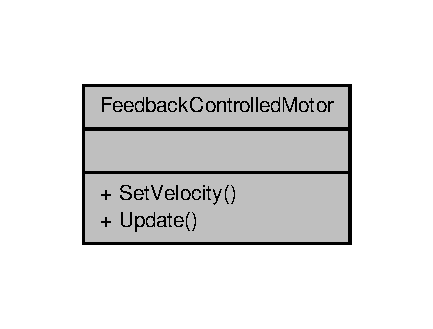
\includegraphics[width=208pt]{class_feedback_controlled_motor__coll__graph}
\end{center}
\end{figure}
\subsection*{Public Member Functions}
\begin{DoxyCompactItemize}
\item 
virtual void \hyperlink{class_feedback_controlled_motor_a533fbeddd7edc7035d5d374e9f4ad118}{Set\-Velocity} (const float velocity)=0
\item 
virtual void \hyperlink{class_feedback_controlled_motor_a54668f85a8dadb66971ee8c8a76be802}{Update} ()=0
\end{DoxyCompactItemize}


\subsection{Member Function Documentation}
\hypertarget{class_feedback_controlled_motor_a533fbeddd7edc7035d5d374e9f4ad118}{\index{Feedback\-Controlled\-Motor@{Feedback\-Controlled\-Motor}!Set\-Velocity@{Set\-Velocity}}
\index{Set\-Velocity@{Set\-Velocity}!FeedbackControlledMotor@{Feedback\-Controlled\-Motor}}
\subsubsection[{Set\-Velocity}]{\setlength{\rightskip}{0pt plus 5cm}virtual void Feedback\-Controlled\-Motor\-::\-Set\-Velocity (
\begin{DoxyParamCaption}
\item[{const float}]{velocity}
\end{DoxyParamCaption}
)\hspace{0.3cm}{\ttfamily [pure virtual]}}}\label{class_feedback_controlled_motor_a533fbeddd7edc7035d5d374e9f4ad118}


Implemented in \hyperlink{class_p_i_d_controlled_motor_a045762a3ef93b7b25a6339cda504e4e5}{P\-I\-D\-Controlled\-Motor}, and \hyperlink{class_mock_p_i_d_motor_a519d3034d3f1b5e7c74d9f9acab9e771}{Mock\-P\-I\-D\-Motor}.



Here is the caller graph for this function\-:\nopagebreak
\begin{figure}[H]
\begin{center}
\leavevmode
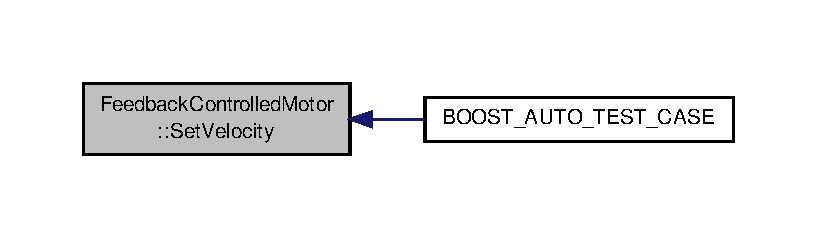
\includegraphics[width=350pt]{class_feedback_controlled_motor_a533fbeddd7edc7035d5d374e9f4ad118_icgraph}
\end{center}
\end{figure}


\hypertarget{class_feedback_controlled_motor_a54668f85a8dadb66971ee8c8a76be802}{\index{Feedback\-Controlled\-Motor@{Feedback\-Controlled\-Motor}!Update@{Update}}
\index{Update@{Update}!FeedbackControlledMotor@{Feedback\-Controlled\-Motor}}
\subsubsection[{Update}]{\setlength{\rightskip}{0pt plus 5cm}virtual void Feedback\-Controlled\-Motor\-::\-Update (
\begin{DoxyParamCaption}
{}
\end{DoxyParamCaption}
)\hspace{0.3cm}{\ttfamily [pure virtual]}}}\label{class_feedback_controlled_motor_a54668f85a8dadb66971ee8c8a76be802}


Implemented in \hyperlink{class_p_i_d_controlled_motor_a7ab5288c0d1df6540475634c9a150df2}{P\-I\-D\-Controlled\-Motor}, and \hyperlink{class_mock_p_i_d_motor_a55a351cb26bd8adf632c97430d60de9f}{Mock\-P\-I\-D\-Motor}.



Here is the caller graph for this function\-:
\nopagebreak
\begin{figure}[H]
\begin{center}
\leavevmode
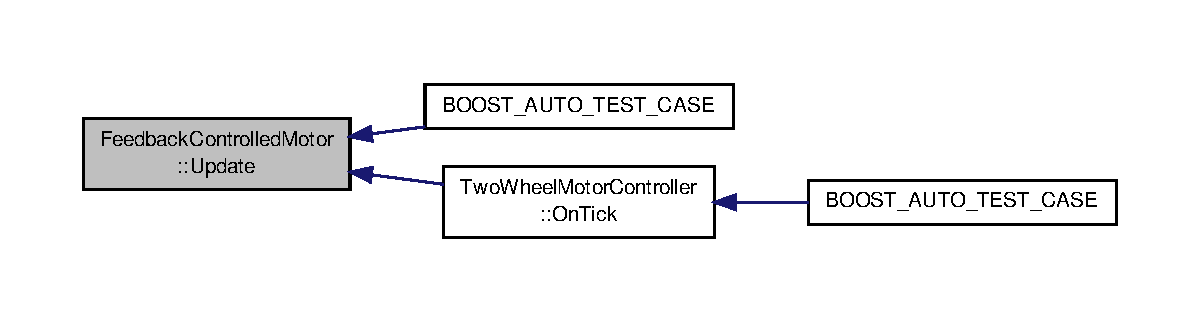
\includegraphics[width=350pt]{class_feedback_controlled_motor_a54668f85a8dadb66971ee8c8a76be802_icgraph}
\end{center}
\end{figure}




The documentation for this class was generated from the following file\-:\begin{DoxyCompactItemize}
\item 
lib/motor\-\_\-control/\hyperlink{_feedback_controlled_motor_8h}{Feedback\-Controlled\-Motor.\-h}\end{DoxyCompactItemize}

\hypertarget{struct_invalid_pin_value_exception}{\section{Invalid\-Pin\-Value\-Exception Struct Reference}
\label{struct_invalid_pin_value_exception}\index{Invalid\-Pin\-Value\-Exception@{Invalid\-Pin\-Value\-Exception}}
}


{\ttfamily \#include $<$Mock\-W\-Program.\-hpp$>$}



Inheritance diagram for Invalid\-Pin\-Value\-Exception\-:\nopagebreak
\begin{figure}[H]
\begin{center}
\leavevmode
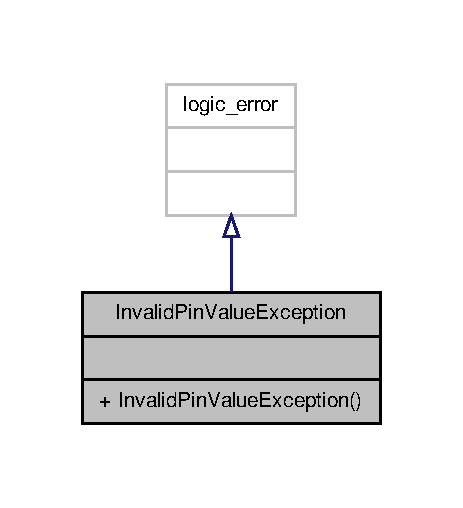
\includegraphics[width=222pt]{struct_invalid_pin_value_exception__inherit__graph}
\end{center}
\end{figure}


Collaboration diagram for Invalid\-Pin\-Value\-Exception\-:\nopagebreak
\begin{figure}[H]
\begin{center}
\leavevmode
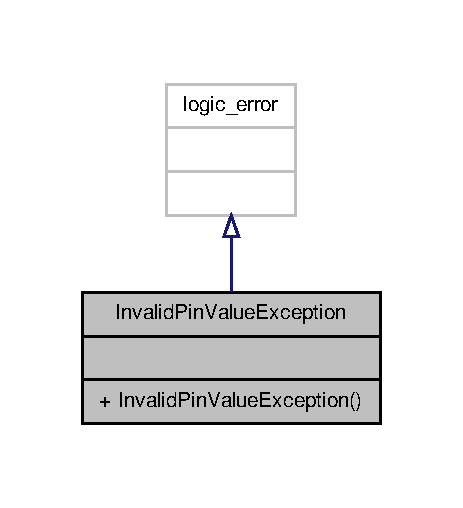
\includegraphics[width=222pt]{struct_invalid_pin_value_exception__coll__graph}
\end{center}
\end{figure}
\subsection*{Public Member Functions}
\begin{DoxyCompactItemize}
\item 
\hyperlink{struct_invalid_pin_value_exception_aaef43d4b680ac15b05e27cc9289761af}{Invalid\-Pin\-Value\-Exception} ()
\end{DoxyCompactItemize}


\subsection{Constructor \& Destructor Documentation}
\hypertarget{struct_invalid_pin_value_exception_aaef43d4b680ac15b05e27cc9289761af}{\index{Invalid\-Pin\-Value\-Exception@{Invalid\-Pin\-Value\-Exception}!Invalid\-Pin\-Value\-Exception@{Invalid\-Pin\-Value\-Exception}}
\index{Invalid\-Pin\-Value\-Exception@{Invalid\-Pin\-Value\-Exception}!InvalidPinValueException@{Invalid\-Pin\-Value\-Exception}}
\subsubsection[{Invalid\-Pin\-Value\-Exception}]{\setlength{\rightskip}{0pt plus 5cm}Invalid\-Pin\-Value\-Exception\-::\-Invalid\-Pin\-Value\-Exception (
\begin{DoxyParamCaption}
{}
\end{DoxyParamCaption}
)\hspace{0.3cm}{\ttfamily [inline]}}}\label{struct_invalid_pin_value_exception_aaef43d4b680ac15b05e27cc9289761af}


The documentation for this struct was generated from the following file\-:\begin{DoxyCompactItemize}
\item 
lib/arduino\-\_\-mocks/\hyperlink{_mock_w_program_8hpp}{Mock\-W\-Program.\-hpp}\end{DoxyCompactItemize}

\hypertarget{struct_invalid_value_exception}{\section{Invalid\-Value\-Exception Struct Reference}
\label{struct_invalid_value_exception}\index{Invalid\-Value\-Exception@{Invalid\-Value\-Exception}}
}


{\ttfamily \#include $<$Mock\-W\-Program.\-hpp$>$}



Inheritance diagram for Invalid\-Value\-Exception\-:\nopagebreak
\begin{figure}[H]
\begin{center}
\leavevmode
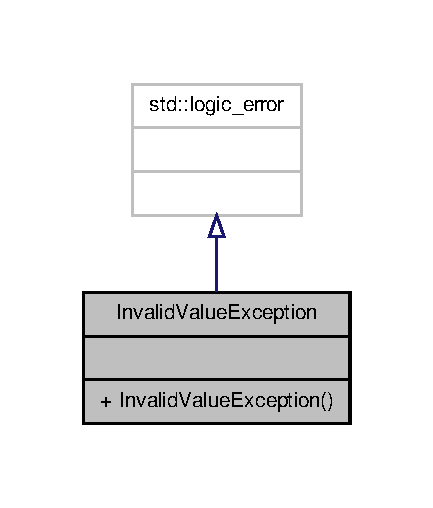
\includegraphics[width=208pt]{struct_invalid_value_exception__inherit__graph}
\end{center}
\end{figure}


Collaboration diagram for Invalid\-Value\-Exception\-:\nopagebreak
\begin{figure}[H]
\begin{center}
\leavevmode
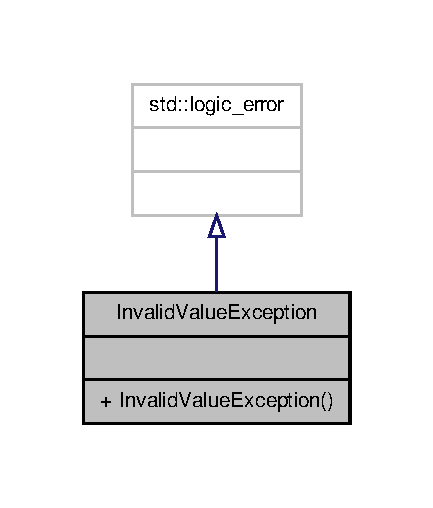
\includegraphics[width=208pt]{struct_invalid_value_exception__coll__graph}
\end{center}
\end{figure}
\subsection*{Public Member Functions}
\begin{DoxyCompactItemize}
\item 
\hyperlink{struct_invalid_value_exception_a7d8a4675bf55b3ee4fb0d80ac9f6ec0b}{Invalid\-Value\-Exception} ()
\end{DoxyCompactItemize}


\subsection{Constructor \& Destructor Documentation}
\hypertarget{struct_invalid_value_exception_a7d8a4675bf55b3ee4fb0d80ac9f6ec0b}{\index{Invalid\-Value\-Exception@{Invalid\-Value\-Exception}!Invalid\-Value\-Exception@{Invalid\-Value\-Exception}}
\index{Invalid\-Value\-Exception@{Invalid\-Value\-Exception}!InvalidValueException@{Invalid\-Value\-Exception}}
\subsubsection[{Invalid\-Value\-Exception}]{\setlength{\rightskip}{0pt plus 5cm}Invalid\-Value\-Exception\-::\-Invalid\-Value\-Exception (
\begin{DoxyParamCaption}
{}
\end{DoxyParamCaption}
)\hspace{0.3cm}{\ttfamily [inline]}}}\label{struct_invalid_value_exception_a7d8a4675bf55b3ee4fb0d80ac9f6ec0b}


The documentation for this struct was generated from the following file\-:\begin{DoxyCompactItemize}
\item 
lib/arduino\-\_\-mocks/\hyperlink{_mock_w_program_8hpp}{Mock\-W\-Program.\-hpp}\end{DoxyCompactItemize}

\hypertarget{class_mock_encoder}{\section{Mock\-Encoder Class Reference}
\label{class_mock_encoder}\index{Mock\-Encoder@{Mock\-Encoder}}
}


{\ttfamily \#include $<$Mock\-Encoder.\-h$>$}



Inheritance diagram for Mock\-Encoder\-:
\nopagebreak
\begin{figure}[H]
\begin{center}
\leavevmode
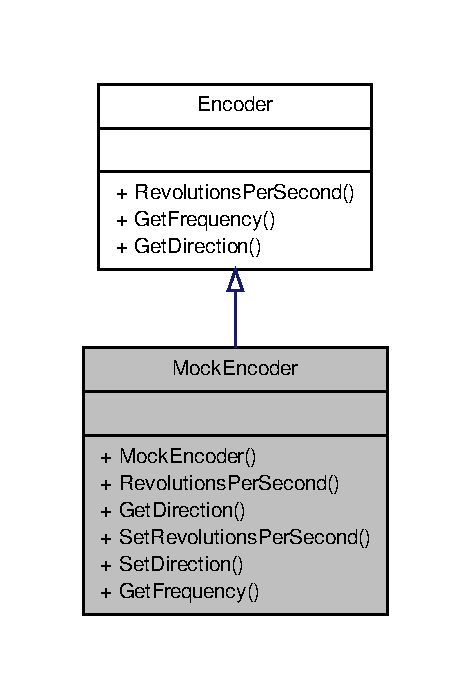
\includegraphics[width=226pt]{class_mock_encoder__inherit__graph}
\end{center}
\end{figure}


Collaboration diagram for Mock\-Encoder\-:
\nopagebreak
\begin{figure}[H]
\begin{center}
\leavevmode
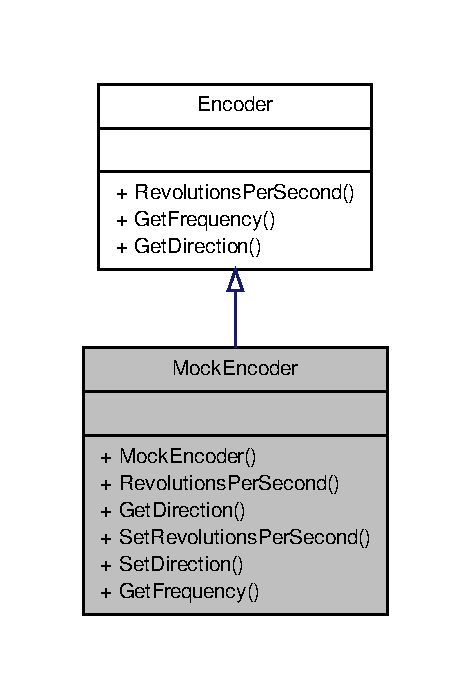
\includegraphics[width=226pt]{class_mock_encoder__coll__graph}
\end{center}
\end{figure}
\subsection*{Public Member Functions}
\begin{DoxyCompactItemize}
\item 
\hyperlink{class_mock_encoder_aa3f65852bafc747d3db73a88354b77c9}{Mock\-Encoder} ()
\item 
float \hyperlink{class_mock_encoder_ad44313dd4a038f09084f04c908fa9a00}{Revolutions\-Per\-Second} ()
\item 
\hyperlink{class_encoder_aa7c4648a7ebc9e651c25c2d450a58213}{Direction} \hyperlink{class_mock_encoder_a167ec4aad9f3f00217c25cec301f26b3}{Get\-Direction} () const 
\item 
void \hyperlink{class_mock_encoder_af26e227ff275c68e4b53d7cdb8eb198c}{Set\-Revolutions\-Per\-Second} (const float new\-Frequency)
\item 
void \hyperlink{class_mock_encoder_a8b3c37c202dae06de65f9481f1799313}{Set\-Direction} (const \hyperlink{class_encoder_aa7c4648a7ebc9e651c25c2d450a58213}{Direction} direction)
\item 
float \hyperlink{class_mock_encoder_a586614c42fbf173f3809dea3e1b9c126}{Get\-Frequency} ()
\end{DoxyCompactItemize}
\subsection*{Additional Inherited Members}


\subsection{Constructor \& Destructor Documentation}
\hypertarget{class_mock_encoder_aa3f65852bafc747d3db73a88354b77c9}{\index{Mock\-Encoder@{Mock\-Encoder}!Mock\-Encoder@{Mock\-Encoder}}
\index{Mock\-Encoder@{Mock\-Encoder}!MockEncoder@{Mock\-Encoder}}
\subsubsection[{Mock\-Encoder}]{\setlength{\rightskip}{0pt plus 5cm}Mock\-Encoder\-::\-Mock\-Encoder (
\begin{DoxyParamCaption}
{}
\end{DoxyParamCaption}
)\hspace{0.3cm}{\ttfamily [inline]}}}\label{class_mock_encoder_aa3f65852bafc747d3db73a88354b77c9}


\subsection{Member Function Documentation}
\hypertarget{class_mock_encoder_a167ec4aad9f3f00217c25cec301f26b3}{\index{Mock\-Encoder@{Mock\-Encoder}!Get\-Direction@{Get\-Direction}}
\index{Get\-Direction@{Get\-Direction}!MockEncoder@{Mock\-Encoder}}
\subsubsection[{Get\-Direction}]{\setlength{\rightskip}{0pt plus 5cm}{\bf Direction} Mock\-Encoder\-::\-Get\-Direction (
\begin{DoxyParamCaption}
{}
\end{DoxyParamCaption}
) const\hspace{0.3cm}{\ttfamily [inline]}, {\ttfamily [virtual]}}}\label{class_mock_encoder_a167ec4aad9f3f00217c25cec301f26b3}


Implements \hyperlink{class_encoder_ab4faff630f313bc0e5b8718df3175fe1}{Encoder}.



Here is the caller graph for this function\-:\nopagebreak
\begin{figure}[H]
\begin{center}
\leavevmode
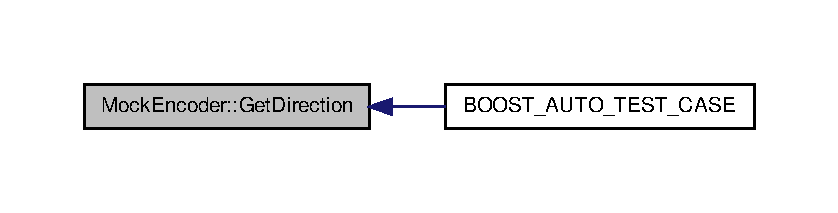
\includegraphics[width=350pt]{class_mock_encoder_a167ec4aad9f3f00217c25cec301f26b3_icgraph}
\end{center}
\end{figure}


\hypertarget{class_mock_encoder_a586614c42fbf173f3809dea3e1b9c126}{\index{Mock\-Encoder@{Mock\-Encoder}!Get\-Frequency@{Get\-Frequency}}
\index{Get\-Frequency@{Get\-Frequency}!MockEncoder@{Mock\-Encoder}}
\subsubsection[{Get\-Frequency}]{\setlength{\rightskip}{0pt plus 5cm}float Mock\-Encoder\-::\-Get\-Frequency (
\begin{DoxyParamCaption}
{}
\end{DoxyParamCaption}
)\hspace{0.3cm}{\ttfamily [inline]}, {\ttfamily [virtual]}}}\label{class_mock_encoder_a586614c42fbf173f3809dea3e1b9c126}


Implements \hyperlink{class_encoder_ab52587693b386731fcdef289e590fc40}{Encoder}.

\hypertarget{class_mock_encoder_ad44313dd4a038f09084f04c908fa9a00}{\index{Mock\-Encoder@{Mock\-Encoder}!Revolutions\-Per\-Second@{Revolutions\-Per\-Second}}
\index{Revolutions\-Per\-Second@{Revolutions\-Per\-Second}!MockEncoder@{Mock\-Encoder}}
\subsubsection[{Revolutions\-Per\-Second}]{\setlength{\rightskip}{0pt plus 5cm}float Mock\-Encoder\-::\-Revolutions\-Per\-Second (
\begin{DoxyParamCaption}
{}
\end{DoxyParamCaption}
)\hspace{0.3cm}{\ttfamily [inline]}, {\ttfamily [virtual]}}}\label{class_mock_encoder_ad44313dd4a038f09084f04c908fa9a00}


Implements \hyperlink{class_encoder_a758adfad11078f8dec0ca672929a4189}{Encoder}.



Here is the caller graph for this function\-:\nopagebreak
\begin{figure}[H]
\begin{center}
\leavevmode
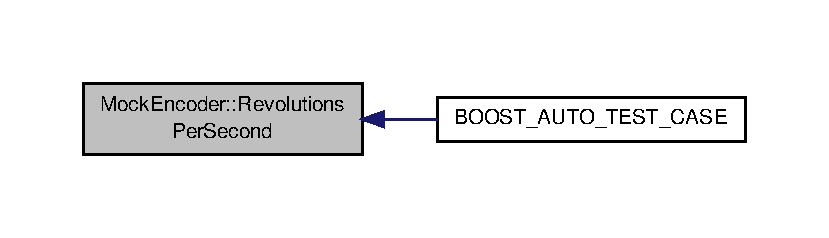
\includegraphics[width=350pt]{class_mock_encoder_ad44313dd4a038f09084f04c908fa9a00_icgraph}
\end{center}
\end{figure}


\hypertarget{class_mock_encoder_a8b3c37c202dae06de65f9481f1799313}{\index{Mock\-Encoder@{Mock\-Encoder}!Set\-Direction@{Set\-Direction}}
\index{Set\-Direction@{Set\-Direction}!MockEncoder@{Mock\-Encoder}}
\subsubsection[{Set\-Direction}]{\setlength{\rightskip}{0pt plus 5cm}void Mock\-Encoder\-::\-Set\-Direction (
\begin{DoxyParamCaption}
\item[{const {\bf Direction}}]{direction}
\end{DoxyParamCaption}
)\hspace{0.3cm}{\ttfamily [inline]}}}\label{class_mock_encoder_a8b3c37c202dae06de65f9481f1799313}


Here is the caller graph for this function\-:\nopagebreak
\begin{figure}[H]
\begin{center}
\leavevmode
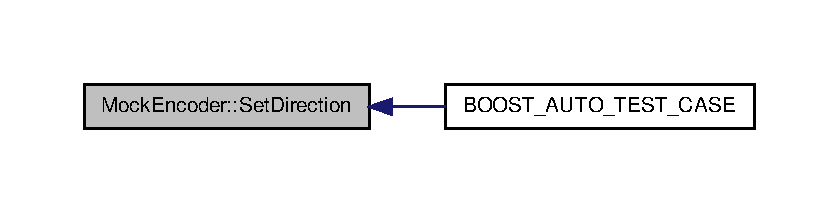
\includegraphics[width=350pt]{class_mock_encoder_a8b3c37c202dae06de65f9481f1799313_icgraph}
\end{center}
\end{figure}


\hypertarget{class_mock_encoder_af26e227ff275c68e4b53d7cdb8eb198c}{\index{Mock\-Encoder@{Mock\-Encoder}!Set\-Revolutions\-Per\-Second@{Set\-Revolutions\-Per\-Second}}
\index{Set\-Revolutions\-Per\-Second@{Set\-Revolutions\-Per\-Second}!MockEncoder@{Mock\-Encoder}}
\subsubsection[{Set\-Revolutions\-Per\-Second}]{\setlength{\rightskip}{0pt plus 5cm}void Mock\-Encoder\-::\-Set\-Revolutions\-Per\-Second (
\begin{DoxyParamCaption}
\item[{const float}]{new\-Frequency}
\end{DoxyParamCaption}
)\hspace{0.3cm}{\ttfamily [inline]}}}\label{class_mock_encoder_af26e227ff275c68e4b53d7cdb8eb198c}


Here is the caller graph for this function\-:\nopagebreak
\begin{figure}[H]
\begin{center}
\leavevmode
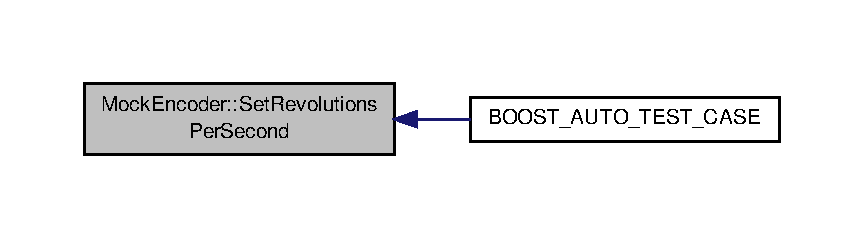
\includegraphics[width=350pt]{class_mock_encoder_af26e227ff275c68e4b53d7cdb8eb198c_icgraph}
\end{center}
\end{figure}




The documentation for this class was generated from the following file\-:\begin{DoxyCompactItemize}
\item 
lib/odometry/test/\hyperlink{_mock_encoder_8h}{Mock\-Encoder.\-h}\end{DoxyCompactItemize}

\hypertarget{class_mock_p_i_d_motor}{\section{Mock\-P\-I\-D\-Motor Class Reference}
\label{class_mock_p_i_d_motor}\index{Mock\-P\-I\-D\-Motor@{Mock\-P\-I\-D\-Motor}}
}


{\ttfamily \#include $<$Mock\-P\-I\-D\-Motor.\-h$>$}



Inheritance diagram for Mock\-P\-I\-D\-Motor\-:
\nopagebreak
\begin{figure}[H]
\begin{center}
\leavevmode
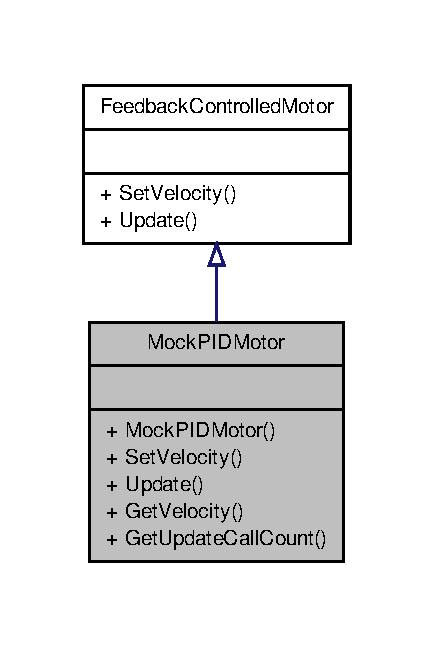
\includegraphics[width=208pt]{class_mock_p_i_d_motor__inherit__graph}
\end{center}
\end{figure}


Collaboration diagram for Mock\-P\-I\-D\-Motor\-:
\nopagebreak
\begin{figure}[H]
\begin{center}
\leavevmode
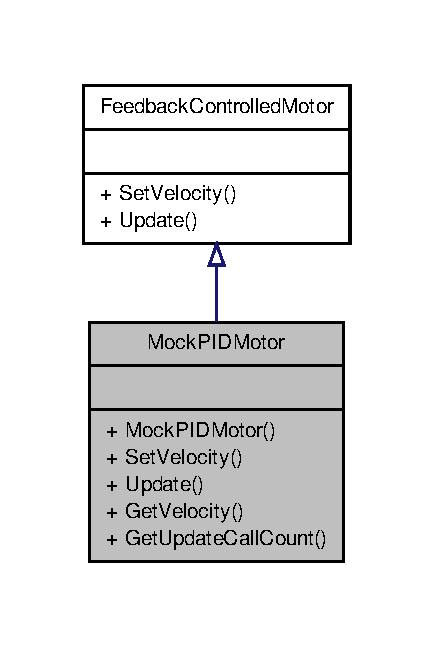
\includegraphics[width=208pt]{class_mock_p_i_d_motor__coll__graph}
\end{center}
\end{figure}
\subsection*{Public Member Functions}
\begin{DoxyCompactItemize}
\item 
\hyperlink{class_mock_p_i_d_motor_a663b3f600d314afe57fa0c19da3ea958}{Mock\-P\-I\-D\-Motor} ()
\item 
void \hyperlink{class_mock_p_i_d_motor_a519d3034d3f1b5e7c74d9f9acab9e771}{Set\-Velocity} (const float velocity)
\item 
void \hyperlink{class_mock_p_i_d_motor_a55a351cb26bd8adf632c97430d60de9f}{Update} ()
\item 
float \hyperlink{class_mock_p_i_d_motor_ad554cf7a3e68830c9607fd587379f557}{Get\-Velocity} () const 
\item 
int \hyperlink{class_mock_p_i_d_motor_af3357dd729cb90a594da62c374c3e3d3}{Get\-Update\-Call\-Count} () const 
\end{DoxyCompactItemize}


\subsection{Constructor \& Destructor Documentation}
\hypertarget{class_mock_p_i_d_motor_a663b3f600d314afe57fa0c19da3ea958}{\index{Mock\-P\-I\-D\-Motor@{Mock\-P\-I\-D\-Motor}!Mock\-P\-I\-D\-Motor@{Mock\-P\-I\-D\-Motor}}
\index{Mock\-P\-I\-D\-Motor@{Mock\-P\-I\-D\-Motor}!MockPIDMotor@{Mock\-P\-I\-D\-Motor}}
\subsubsection[{Mock\-P\-I\-D\-Motor}]{\setlength{\rightskip}{0pt plus 5cm}Mock\-P\-I\-D\-Motor\-::\-Mock\-P\-I\-D\-Motor (
\begin{DoxyParamCaption}
{}
\end{DoxyParamCaption}
)\hspace{0.3cm}{\ttfamily [inline]}}}\label{class_mock_p_i_d_motor_a663b3f600d314afe57fa0c19da3ea958}


\subsection{Member Function Documentation}
\hypertarget{class_mock_p_i_d_motor_af3357dd729cb90a594da62c374c3e3d3}{\index{Mock\-P\-I\-D\-Motor@{Mock\-P\-I\-D\-Motor}!Get\-Update\-Call\-Count@{Get\-Update\-Call\-Count}}
\index{Get\-Update\-Call\-Count@{Get\-Update\-Call\-Count}!MockPIDMotor@{Mock\-P\-I\-D\-Motor}}
\subsubsection[{Get\-Update\-Call\-Count}]{\setlength{\rightskip}{0pt plus 5cm}int Mock\-P\-I\-D\-Motor\-::\-Get\-Update\-Call\-Count (
\begin{DoxyParamCaption}
{}
\end{DoxyParamCaption}
) const\hspace{0.3cm}{\ttfamily [inline]}}}\label{class_mock_p_i_d_motor_af3357dd729cb90a594da62c374c3e3d3}


Here is the caller graph for this function\-:\nopagebreak
\begin{figure}[H]
\begin{center}
\leavevmode
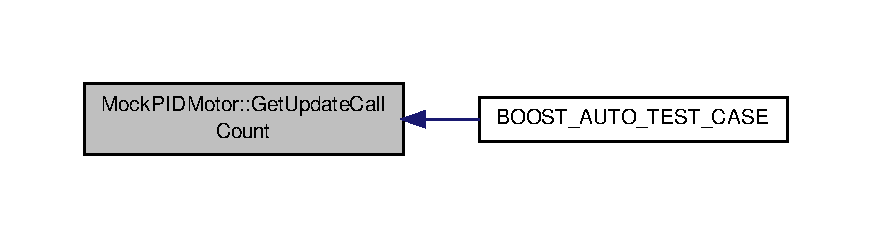
\includegraphics[width=350pt]{class_mock_p_i_d_motor_af3357dd729cb90a594da62c374c3e3d3_icgraph}
\end{center}
\end{figure}


\hypertarget{class_mock_p_i_d_motor_ad554cf7a3e68830c9607fd587379f557}{\index{Mock\-P\-I\-D\-Motor@{Mock\-P\-I\-D\-Motor}!Get\-Velocity@{Get\-Velocity}}
\index{Get\-Velocity@{Get\-Velocity}!MockPIDMotor@{Mock\-P\-I\-D\-Motor}}
\subsubsection[{Get\-Velocity}]{\setlength{\rightskip}{0pt plus 5cm}float Mock\-P\-I\-D\-Motor\-::\-Get\-Velocity (
\begin{DoxyParamCaption}
{}
\end{DoxyParamCaption}
) const\hspace{0.3cm}{\ttfamily [inline]}}}\label{class_mock_p_i_d_motor_ad554cf7a3e68830c9607fd587379f557}


Here is the caller graph for this function\-:\nopagebreak
\begin{figure}[H]
\begin{center}
\leavevmode
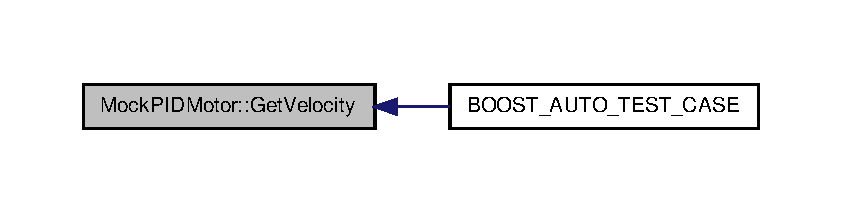
\includegraphics[width=350pt]{class_mock_p_i_d_motor_ad554cf7a3e68830c9607fd587379f557_icgraph}
\end{center}
\end{figure}


\hypertarget{class_mock_p_i_d_motor_a519d3034d3f1b5e7c74d9f9acab9e771}{\index{Mock\-P\-I\-D\-Motor@{Mock\-P\-I\-D\-Motor}!Set\-Velocity@{Set\-Velocity}}
\index{Set\-Velocity@{Set\-Velocity}!MockPIDMotor@{Mock\-P\-I\-D\-Motor}}
\subsubsection[{Set\-Velocity}]{\setlength{\rightskip}{0pt plus 5cm}void Mock\-P\-I\-D\-Motor\-::\-Set\-Velocity (
\begin{DoxyParamCaption}
\item[{const float}]{velocity}
\end{DoxyParamCaption}
)\hspace{0.3cm}{\ttfamily [inline]}, {\ttfamily [virtual]}}}\label{class_mock_p_i_d_motor_a519d3034d3f1b5e7c74d9f9acab9e771}


Implements \hyperlink{class_feedback_controlled_motor_a533fbeddd7edc7035d5d374e9f4ad118}{Feedback\-Controlled\-Motor}.

\hypertarget{class_mock_p_i_d_motor_a55a351cb26bd8adf632c97430d60de9f}{\index{Mock\-P\-I\-D\-Motor@{Mock\-P\-I\-D\-Motor}!Update@{Update}}
\index{Update@{Update}!MockPIDMotor@{Mock\-P\-I\-D\-Motor}}
\subsubsection[{Update}]{\setlength{\rightskip}{0pt plus 5cm}void Mock\-P\-I\-D\-Motor\-::\-Update (
\begin{DoxyParamCaption}
{}
\end{DoxyParamCaption}
)\hspace{0.3cm}{\ttfamily [inline]}, {\ttfamily [virtual]}}}\label{class_mock_p_i_d_motor_a55a351cb26bd8adf632c97430d60de9f}


Implements \hyperlink{class_feedback_controlled_motor_a54668f85a8dadb66971ee8c8a76be802}{Feedback\-Controlled\-Motor}.



The documentation for this class was generated from the following file\-:\begin{DoxyCompactItemize}
\item 
lib/motor\-\_\-control/test/\hyperlink{_mock_p_i_d_motor_8h}{Mock\-P\-I\-D\-Motor.\-h}\end{DoxyCompactItemize}

\hypertarget{class_mock_serial}{\section{Mock\-Serial Class Reference}
\label{class_mock_serial}\index{Mock\-Serial@{Mock\-Serial}}
}


{\ttfamily \#include $<$Mock\-W\-Program.\-hpp$>$}



Collaboration diagram for Mock\-Serial\-:\nopagebreak
\begin{figure}[H]
\begin{center}
\leavevmode
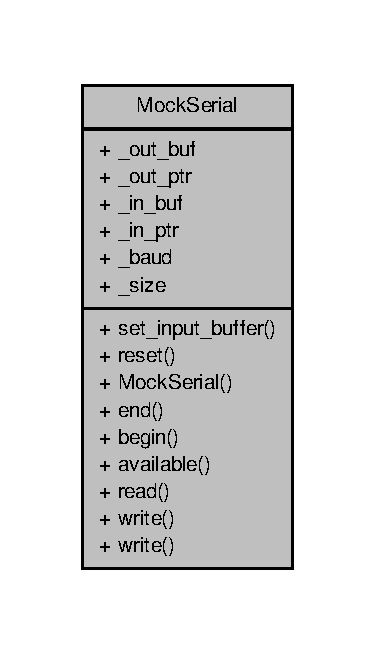
\includegraphics[width=180pt]{class_mock_serial__coll__graph}
\end{center}
\end{figure}
\subsection*{Public Member Functions}
\begin{DoxyCompactItemize}
\item 
void \hyperlink{class_mock_serial_a48e85d202f87e4b8cd5309b022f38cf6}{set\-\_\-input\-\_\-buffer} (uint8\-\_\-t $\ast$new\-\_\-buf, uint16\-\_\-t size)
\begin{DoxyCompactList}\small\item\em Set the input buffer data. \end{DoxyCompactList}\item 
void \hyperlink{class_mock_serial_a12583e99c566cf006102367830a88495}{reset} (void)
\item 
\hyperlink{class_mock_serial_a59607f7ccbb19c4d1d6f89370dc65468}{Mock\-Serial} ()
\item 
void \hyperlink{class_mock_serial_a4cb7a5cdda45fa933d7cc9414b404b18}{end} (void)
\item 
void \hyperlink{class_mock_serial_a094ec60b8ccc49ce444e2abfc9de4396}{begin} (uint32\-\_\-t baud)
\begin{DoxyCompactList}\small\item\em Begin serial communications. \end{DoxyCompactList}\item 
uint32\-\_\-t \hyperlink{class_mock_serial_a590ebe7857593eeeabed3bbef6eb0906}{available} ()
\begin{DoxyCompactList}\small\item\em Check the number of bytes available in the input buffer. \end{DoxyCompactList}\item 
int \hyperlink{class_mock_serial_a24882d7f86bed46d72dce80abc7ff49b}{read} ()
\begin{DoxyCompactList}\small\item\em Read a byte from the input buffer. \end{DoxyCompactList}\item 
void \hyperlink{class_mock_serial_aa10ceb982bfbc533d94fbd0558d5c0a6}{write} (uint8\-\_\-t value)
\begin{DoxyCompactList}\small\item\em Write a byte to the output buffer. \end{DoxyCompactList}\item 
void \hyperlink{class_mock_serial_a98bdd77ce2c62ad05e271d828bbb81b2}{write} (uint8\-\_\-t $\ast$values, uint32\-\_\-t length)
\begin{DoxyCompactList}\small\item\em Write a byte array to the output buffer. \end{DoxyCompactList}\end{DoxyCompactItemize}
\subsection*{Public Attributes}
\begin{DoxyCompactItemize}
\item 
uint8\-\_\-t $\ast$ \hyperlink{class_mock_serial_af89e1c5936fd7d382175ae57a5c34bf6}{\-\_\-out\-\_\-buf}
\item 
uint16\-\_\-t \hyperlink{class_mock_serial_a0d4616ef10a3e6dbac58922ef972a448}{\-\_\-out\-\_\-ptr}
\item 
uint8\-\_\-t $\ast$ \hyperlink{class_mock_serial_a5516617e3418d21180c2f2c0cb3dbd15}{\-\_\-in\-\_\-buf}
\item 
uint16\-\_\-t \hyperlink{class_mock_serial_a4c3f74b6cef52501833158c064395b0a}{\-\_\-in\-\_\-ptr}
\item 
uint32\-\_\-t \hyperlink{class_mock_serial_abbb8ad8b05cf475e6e34ba591a753146}{\-\_\-baud}
\item 
uint16\-\_\-t \hyperlink{class_mock_serial_a2a26571f236f963d4d1e87cc17d75bda}{\-\_\-size}
\end{DoxyCompactItemize}


\subsection{Constructor \& Destructor Documentation}
\hypertarget{class_mock_serial_a59607f7ccbb19c4d1d6f89370dc65468}{\index{Mock\-Serial@{Mock\-Serial}!Mock\-Serial@{Mock\-Serial}}
\index{Mock\-Serial@{Mock\-Serial}!MockSerial@{Mock\-Serial}}
\subsubsection[{Mock\-Serial}]{\setlength{\rightskip}{0pt plus 5cm}Mock\-Serial\-::\-Mock\-Serial (
\begin{DoxyParamCaption}
{}
\end{DoxyParamCaption}
)}}\label{class_mock_serial_a59607f7ccbb19c4d1d6f89370dc65468}


Here is the call graph for this function\-:\nopagebreak
\begin{figure}[H]
\begin{center}
\leavevmode
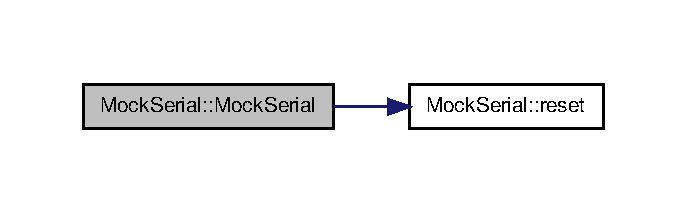
\includegraphics[width=330pt]{class_mock_serial_a59607f7ccbb19c4d1d6f89370dc65468_cgraph}
\end{center}
\end{figure}




\subsection{Member Function Documentation}
\hypertarget{class_mock_serial_a590ebe7857593eeeabed3bbef6eb0906}{\index{Mock\-Serial@{Mock\-Serial}!available@{available}}
\index{available@{available}!MockSerial@{Mock\-Serial}}
\subsubsection[{available}]{\setlength{\rightskip}{0pt plus 5cm}uint32\-\_\-t Mock\-Serial\-::available (
\begin{DoxyParamCaption}
{}
\end{DoxyParamCaption}
)}}\label{class_mock_serial_a590ebe7857593eeeabed3bbef6eb0906}


Check the number of bytes available in the input buffer. 

\begin{DoxyReturn}{Returns}
The number of bytes available for read. 
\end{DoxyReturn}
\hypertarget{class_mock_serial_a094ec60b8ccc49ce444e2abfc9de4396}{\index{Mock\-Serial@{Mock\-Serial}!begin@{begin}}
\index{begin@{begin}!MockSerial@{Mock\-Serial}}
\subsubsection[{begin}]{\setlength{\rightskip}{0pt plus 5cm}void Mock\-Serial\-::begin (
\begin{DoxyParamCaption}
\item[{uint32\-\_\-t}]{baud}
\end{DoxyParamCaption}
)}}\label{class_mock_serial_a094ec60b8ccc49ce444e2abfc9de4396}


Begin serial communications. 

This sets the current baud rate, but is otherwise a no-\/op.


\begin{DoxyParams}{Parameters}
{\em baud} & The baud rate to communicate at. \\
\hline
\end{DoxyParams}
\hypertarget{class_mock_serial_a4cb7a5cdda45fa933d7cc9414b404b18}{\index{Mock\-Serial@{Mock\-Serial}!end@{end}}
\index{end@{end}!MockSerial@{Mock\-Serial}}
\subsubsection[{end}]{\setlength{\rightskip}{0pt plus 5cm}void Mock\-Serial\-::end (
\begin{DoxyParamCaption}
\item[{void}]{}
\end{DoxyParamCaption}
)}}\label{class_mock_serial_a4cb7a5cdda45fa933d7cc9414b404b18}
\hypertarget{class_mock_serial_a24882d7f86bed46d72dce80abc7ff49b}{\index{Mock\-Serial@{Mock\-Serial}!read@{read}}
\index{read@{read}!MockSerial@{Mock\-Serial}}
\subsubsection[{read}]{\setlength{\rightskip}{0pt plus 5cm}int Mock\-Serial\-::read (
\begin{DoxyParamCaption}
{}
\end{DoxyParamCaption}
)}}\label{class_mock_serial_a24882d7f86bed46d72dce80abc7ff49b}


Read a byte from the input buffer. 

\begin{DoxyReturn}{Returns}
The next byte from the input buffer. 
\end{DoxyReturn}
\hypertarget{class_mock_serial_a12583e99c566cf006102367830a88495}{\index{Mock\-Serial@{Mock\-Serial}!reset@{reset}}
\index{reset@{reset}!MockSerial@{Mock\-Serial}}
\subsubsection[{reset}]{\setlength{\rightskip}{0pt plus 5cm}void Mock\-Serial\-::reset (
\begin{DoxyParamCaption}
\item[{void}]{}
\end{DoxyParamCaption}
)}}\label{class_mock_serial_a12583e99c566cf006102367830a88495}


Here is the caller graph for this function\-:\nopagebreak
\begin{figure}[H]
\begin{center}
\leavevmode
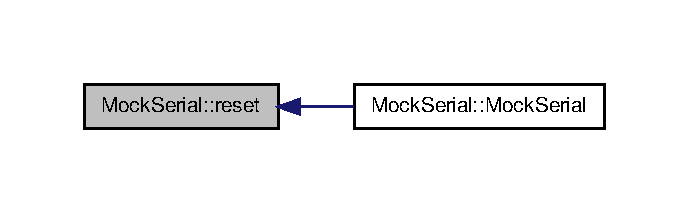
\includegraphics[width=330pt]{class_mock_serial_a12583e99c566cf006102367830a88495_icgraph}
\end{center}
\end{figure}


\hypertarget{class_mock_serial_a48e85d202f87e4b8cd5309b022f38cf6}{\index{Mock\-Serial@{Mock\-Serial}!set\-\_\-input\-\_\-buffer@{set\-\_\-input\-\_\-buffer}}
\index{set\-\_\-input\-\_\-buffer@{set\-\_\-input\-\_\-buffer}!MockSerial@{Mock\-Serial}}
\subsubsection[{set\-\_\-input\-\_\-buffer}]{\setlength{\rightskip}{0pt plus 5cm}void Mock\-Serial\-::set\-\_\-input\-\_\-buffer (
\begin{DoxyParamCaption}
\item[{uint8\-\_\-t $\ast$}]{new\-\_\-buf, }
\item[{uint16\-\_\-t}]{size}
\end{DoxyParamCaption}
)}}\label{class_mock_serial_a48e85d202f87e4b8cd5309b022f38cf6}


Set the input buffer data. 


\begin{DoxyParams}{Parameters}
{\em new\-\_\-buf} & A pointer to a byte array containing the input data. \\
\hline
{\em size} & The size of the input array. \\
\hline
\end{DoxyParams}
\hypertarget{class_mock_serial_aa10ceb982bfbc533d94fbd0558d5c0a6}{\index{Mock\-Serial@{Mock\-Serial}!write@{write}}
\index{write@{write}!MockSerial@{Mock\-Serial}}
\subsubsection[{write}]{\setlength{\rightskip}{0pt plus 5cm}void Mock\-Serial\-::write (
\begin{DoxyParamCaption}
\item[{uint8\-\_\-t}]{value}
\end{DoxyParamCaption}
)}}\label{class_mock_serial_aa10ceb982bfbc533d94fbd0558d5c0a6}


Write a byte to the output buffer. 


\begin{DoxyParams}{Parameters}
{\em value} & The byte to write. \\
\hline
\end{DoxyParams}
\hypertarget{class_mock_serial_a98bdd77ce2c62ad05e271d828bbb81b2}{\index{Mock\-Serial@{Mock\-Serial}!write@{write}}
\index{write@{write}!MockSerial@{Mock\-Serial}}
\subsubsection[{write}]{\setlength{\rightskip}{0pt plus 5cm}void Mock\-Serial\-::write (
\begin{DoxyParamCaption}
\item[{uint8\-\_\-t $\ast$}]{values, }
\item[{uint32\-\_\-t}]{length}
\end{DoxyParamCaption}
)}}\label{class_mock_serial_a98bdd77ce2c62ad05e271d828bbb81b2}


Write a byte array to the output buffer. 


\begin{DoxyParams}{Parameters}
{\em values} & An array of values to write. \\
\hline
{\em length} & The length of the array. \\
\hline
\end{DoxyParams}


\subsection{Member Data Documentation}
\hypertarget{class_mock_serial_abbb8ad8b05cf475e6e34ba591a753146}{\index{Mock\-Serial@{Mock\-Serial}!\-\_\-baud@{\-\_\-baud}}
\index{\-\_\-baud@{\-\_\-baud}!MockSerial@{Mock\-Serial}}
\subsubsection[{\-\_\-baud}]{\setlength{\rightskip}{0pt plus 5cm}uint32\-\_\-t Mock\-Serial\-::\-\_\-baud}}\label{class_mock_serial_abbb8ad8b05cf475e6e34ba591a753146}
\hypertarget{class_mock_serial_a5516617e3418d21180c2f2c0cb3dbd15}{\index{Mock\-Serial@{Mock\-Serial}!\-\_\-in\-\_\-buf@{\-\_\-in\-\_\-buf}}
\index{\-\_\-in\-\_\-buf@{\-\_\-in\-\_\-buf}!MockSerial@{Mock\-Serial}}
\subsubsection[{\-\_\-in\-\_\-buf}]{\setlength{\rightskip}{0pt plus 5cm}uint8\-\_\-t$\ast$ Mock\-Serial\-::\-\_\-in\-\_\-buf}}\label{class_mock_serial_a5516617e3418d21180c2f2c0cb3dbd15}
\hypertarget{class_mock_serial_a4c3f74b6cef52501833158c064395b0a}{\index{Mock\-Serial@{Mock\-Serial}!\-\_\-in\-\_\-ptr@{\-\_\-in\-\_\-ptr}}
\index{\-\_\-in\-\_\-ptr@{\-\_\-in\-\_\-ptr}!MockSerial@{Mock\-Serial}}
\subsubsection[{\-\_\-in\-\_\-ptr}]{\setlength{\rightskip}{0pt plus 5cm}uint16\-\_\-t Mock\-Serial\-::\-\_\-in\-\_\-ptr}}\label{class_mock_serial_a4c3f74b6cef52501833158c064395b0a}
\hypertarget{class_mock_serial_af89e1c5936fd7d382175ae57a5c34bf6}{\index{Mock\-Serial@{Mock\-Serial}!\-\_\-out\-\_\-buf@{\-\_\-out\-\_\-buf}}
\index{\-\_\-out\-\_\-buf@{\-\_\-out\-\_\-buf}!MockSerial@{Mock\-Serial}}
\subsubsection[{\-\_\-out\-\_\-buf}]{\setlength{\rightskip}{0pt plus 5cm}uint8\-\_\-t$\ast$ Mock\-Serial\-::\-\_\-out\-\_\-buf}}\label{class_mock_serial_af89e1c5936fd7d382175ae57a5c34bf6}
\hypertarget{class_mock_serial_a0d4616ef10a3e6dbac58922ef972a448}{\index{Mock\-Serial@{Mock\-Serial}!\-\_\-out\-\_\-ptr@{\-\_\-out\-\_\-ptr}}
\index{\-\_\-out\-\_\-ptr@{\-\_\-out\-\_\-ptr}!MockSerial@{Mock\-Serial}}
\subsubsection[{\-\_\-out\-\_\-ptr}]{\setlength{\rightskip}{0pt plus 5cm}uint16\-\_\-t Mock\-Serial\-::\-\_\-out\-\_\-ptr}}\label{class_mock_serial_a0d4616ef10a3e6dbac58922ef972a448}
\hypertarget{class_mock_serial_a2a26571f236f963d4d1e87cc17d75bda}{\index{Mock\-Serial@{Mock\-Serial}!\-\_\-size@{\-\_\-size}}
\index{\-\_\-size@{\-\_\-size}!MockSerial@{Mock\-Serial}}
\subsubsection[{\-\_\-size}]{\setlength{\rightskip}{0pt plus 5cm}uint16\-\_\-t Mock\-Serial\-::\-\_\-size}}\label{class_mock_serial_a2a26571f236f963d4d1e87cc17d75bda}


The documentation for this class was generated from the following files\-:\begin{DoxyCompactItemize}
\item 
lib/arduino\-\_\-mocks/\hyperlink{_mock_w_program_8hpp}{Mock\-W\-Program.\-hpp}\item 
lib/arduino\-\_\-mocks/\hyperlink{_mock_serial_8cpp}{Mock\-Serial.\-cpp}\end{DoxyCompactItemize}

\hypertarget{class_motor}{\section{Motor Class Reference}
\label{class_motor}\index{Motor@{Motor}}
}


{\ttfamily \#include $<$Motor.\-h$>$}



Collaboration diagram for Motor\-:
\nopagebreak
\begin{figure}[H]
\begin{center}
\leavevmode
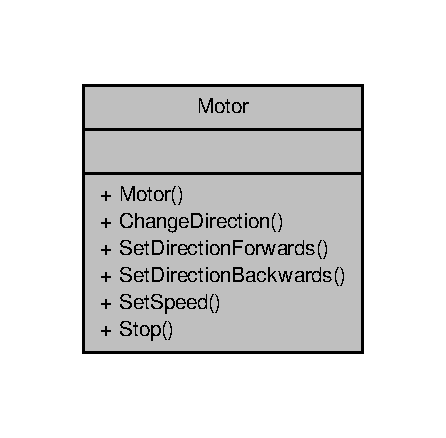
\includegraphics[width=214pt]{class_motor__coll__graph}
\end{center}
\end{figure}
\subsection*{Public Member Functions}
\begin{DoxyCompactItemize}
\item 
\hyperlink{class_motor_a9d515b9ac1a73e1c59143a95884e4c9d}{Motor} (const int direction\-Pin, const int pwm\-Pin)
\item 
void \hyperlink{class_motor_a4b1fb35dcf10c3e17a1614877b9b6a7d}{Change\-Direction} ()
\item 
void \hyperlink{class_motor_aa98ff82632c1be028f76173094fc9eae}{Set\-Direction\-Forwards} ()
\item 
void \hyperlink{class_motor_a81a6ae7005ee0f21fc04d3b8303448f7}{Set\-Direction\-Backwards} ()
\item 
void \hyperlink{class_motor_afe04b2b18bd3e6e300ee14e3648c40bf}{Set\-Speed} (int speed)
\item 
void \hyperlink{class_motor_a8f0fdb6c977ea11e89281c51534850ca}{Stop} ()
\end{DoxyCompactItemize}


\subsection{Constructor \& Destructor Documentation}
\hypertarget{class_motor_a9d515b9ac1a73e1c59143a95884e4c9d}{\index{Motor@{Motor}!Motor@{Motor}}
\index{Motor@{Motor}!Motor@{Motor}}
\subsubsection[{Motor}]{\setlength{\rightskip}{0pt plus 5cm}Motor\-::\-Motor (
\begin{DoxyParamCaption}
\item[{const int}]{direction\-Pin, }
\item[{const int}]{pwm\-Pin}
\end{DoxyParamCaption}
)}}\label{class_motor_a9d515b9ac1a73e1c59143a95884e4c9d}


Here is the call graph for this function\-:
\nopagebreak
\begin{figure}[H]
\begin{center}
\leavevmode
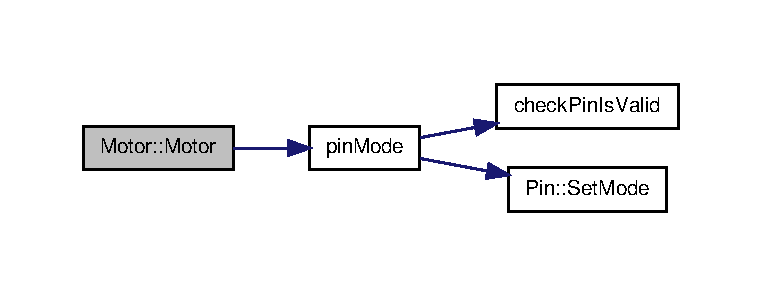
\includegraphics[width=350pt]{class_motor_a9d515b9ac1a73e1c59143a95884e4c9d_cgraph}
\end{center}
\end{figure}




\subsection{Member Function Documentation}
\hypertarget{class_motor_a4b1fb35dcf10c3e17a1614877b9b6a7d}{\index{Motor@{Motor}!Change\-Direction@{Change\-Direction}}
\index{Change\-Direction@{Change\-Direction}!Motor@{Motor}}
\subsubsection[{Change\-Direction}]{\setlength{\rightskip}{0pt plus 5cm}void Motor\-::\-Change\-Direction (
\begin{DoxyParamCaption}
{}
\end{DoxyParamCaption}
)}}\label{class_motor_a4b1fb35dcf10c3e17a1614877b9b6a7d}
\hypertarget{class_motor_a81a6ae7005ee0f21fc04d3b8303448f7}{\index{Motor@{Motor}!Set\-Direction\-Backwards@{Set\-Direction\-Backwards}}
\index{Set\-Direction\-Backwards@{Set\-Direction\-Backwards}!Motor@{Motor}}
\subsubsection[{Set\-Direction\-Backwards}]{\setlength{\rightskip}{0pt plus 5cm}void Motor\-::\-Set\-Direction\-Backwards (
\begin{DoxyParamCaption}
{}
\end{DoxyParamCaption}
)}}\label{class_motor_a81a6ae7005ee0f21fc04d3b8303448f7}


Here is the call graph for this function\-:
\nopagebreak
\begin{figure}[H]
\begin{center}
\leavevmode
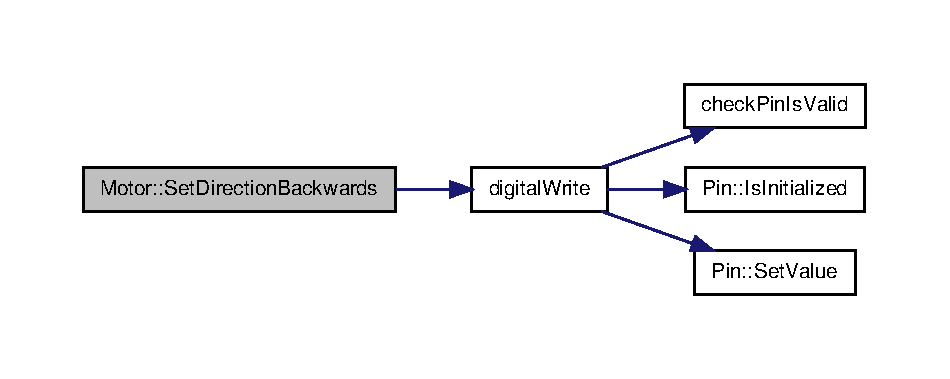
\includegraphics[width=350pt]{class_motor_a81a6ae7005ee0f21fc04d3b8303448f7_cgraph}
\end{center}
\end{figure}




Here is the caller graph for this function\-:
\nopagebreak
\begin{figure}[H]
\begin{center}
\leavevmode
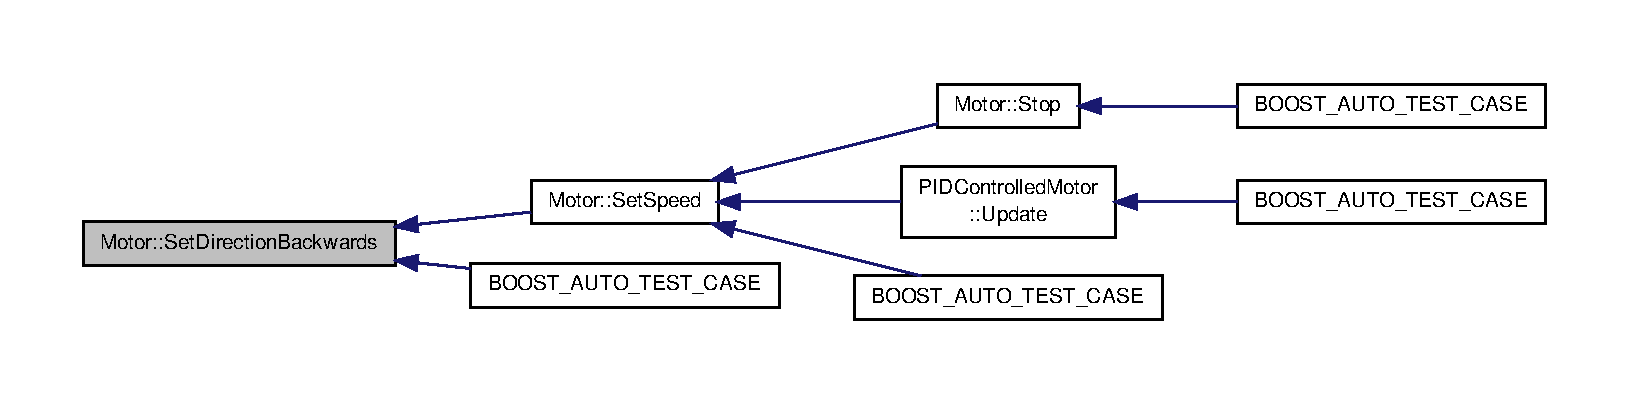
\includegraphics[width=350pt]{class_motor_a81a6ae7005ee0f21fc04d3b8303448f7_icgraph}
\end{center}
\end{figure}


\hypertarget{class_motor_aa98ff82632c1be028f76173094fc9eae}{\index{Motor@{Motor}!Set\-Direction\-Forwards@{Set\-Direction\-Forwards}}
\index{Set\-Direction\-Forwards@{Set\-Direction\-Forwards}!Motor@{Motor}}
\subsubsection[{Set\-Direction\-Forwards}]{\setlength{\rightskip}{0pt plus 5cm}void Motor\-::\-Set\-Direction\-Forwards (
\begin{DoxyParamCaption}
{}
\end{DoxyParamCaption}
)}}\label{class_motor_aa98ff82632c1be028f76173094fc9eae}


Here is the call graph for this function\-:
\nopagebreak
\begin{figure}[H]
\begin{center}
\leavevmode
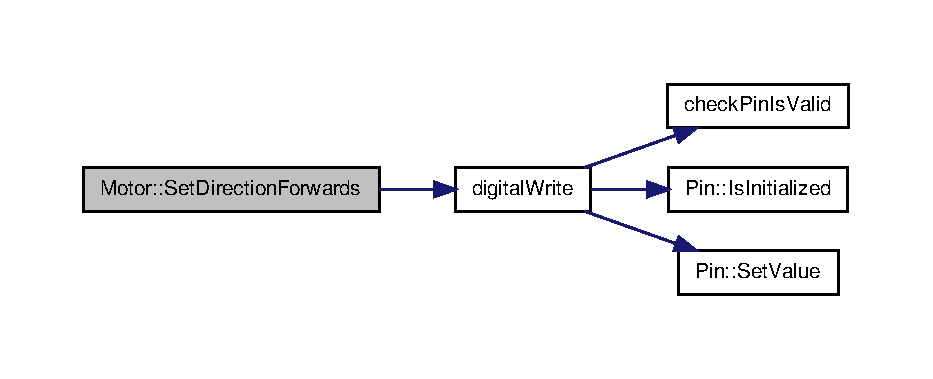
\includegraphics[width=350pt]{class_motor_aa98ff82632c1be028f76173094fc9eae_cgraph}
\end{center}
\end{figure}




Here is the caller graph for this function\-:
\nopagebreak
\begin{figure}[H]
\begin{center}
\leavevmode
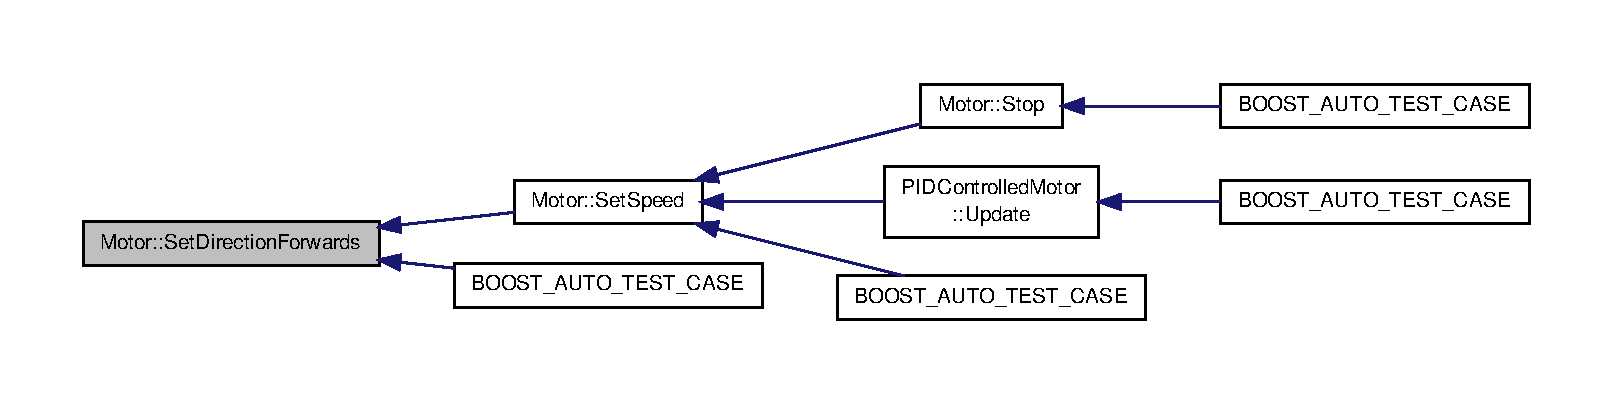
\includegraphics[width=350pt]{class_motor_aa98ff82632c1be028f76173094fc9eae_icgraph}
\end{center}
\end{figure}


\hypertarget{class_motor_afe04b2b18bd3e6e300ee14e3648c40bf}{\index{Motor@{Motor}!Set\-Speed@{Set\-Speed}}
\index{Set\-Speed@{Set\-Speed}!Motor@{Motor}}
\subsubsection[{Set\-Speed}]{\setlength{\rightskip}{0pt plus 5cm}void Motor\-::\-Set\-Speed (
\begin{DoxyParamCaption}
\item[{int}]{speed}
\end{DoxyParamCaption}
)}}\label{class_motor_afe04b2b18bd3e6e300ee14e3648c40bf}


Here is the call graph for this function\-:
\nopagebreak
\begin{figure}[H]
\begin{center}
\leavevmode
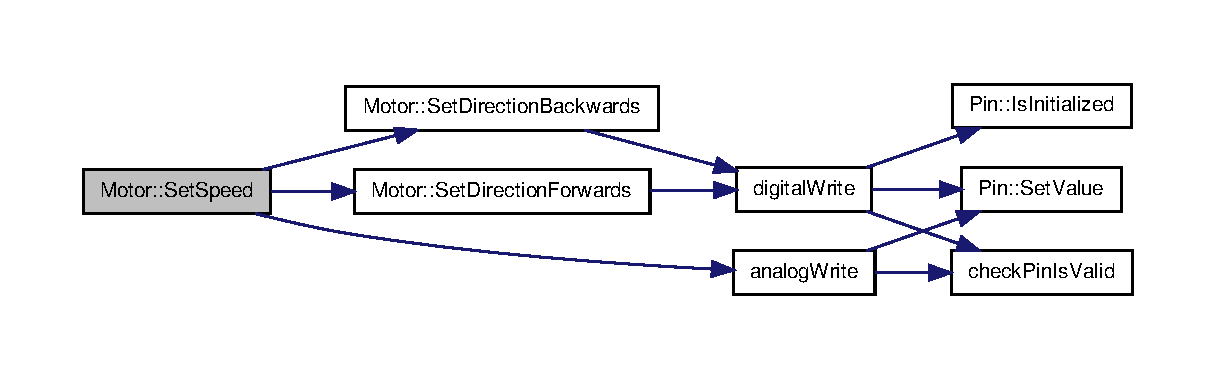
\includegraphics[width=350pt]{class_motor_afe04b2b18bd3e6e300ee14e3648c40bf_cgraph}
\end{center}
\end{figure}




Here is the caller graph for this function\-:
\nopagebreak
\begin{figure}[H]
\begin{center}
\leavevmode
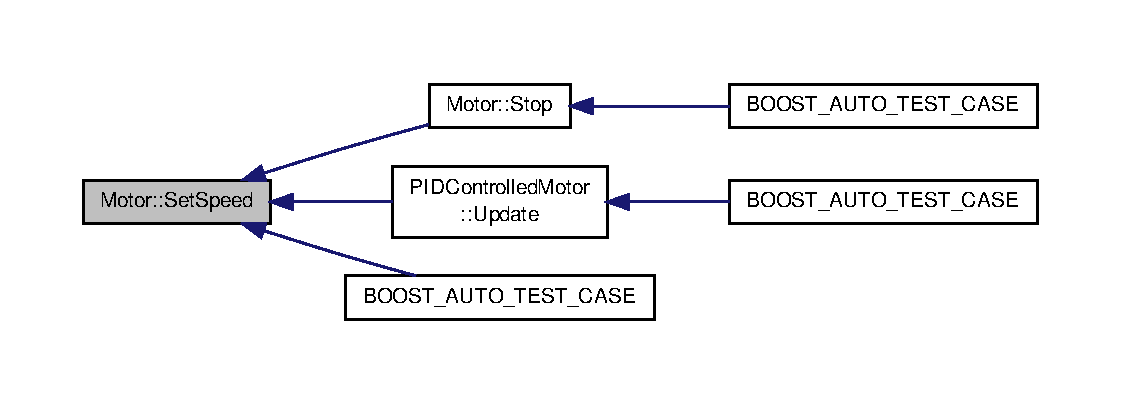
\includegraphics[width=350pt]{class_motor_afe04b2b18bd3e6e300ee14e3648c40bf_icgraph}
\end{center}
\end{figure}


\hypertarget{class_motor_a8f0fdb6c977ea11e89281c51534850ca}{\index{Motor@{Motor}!Stop@{Stop}}
\index{Stop@{Stop}!Motor@{Motor}}
\subsubsection[{Stop}]{\setlength{\rightskip}{0pt plus 5cm}void Motor\-::\-Stop (
\begin{DoxyParamCaption}
{}
\end{DoxyParamCaption}
)}}\label{class_motor_a8f0fdb6c977ea11e89281c51534850ca}


Here is the call graph for this function\-:
\nopagebreak
\begin{figure}[H]
\begin{center}
\leavevmode
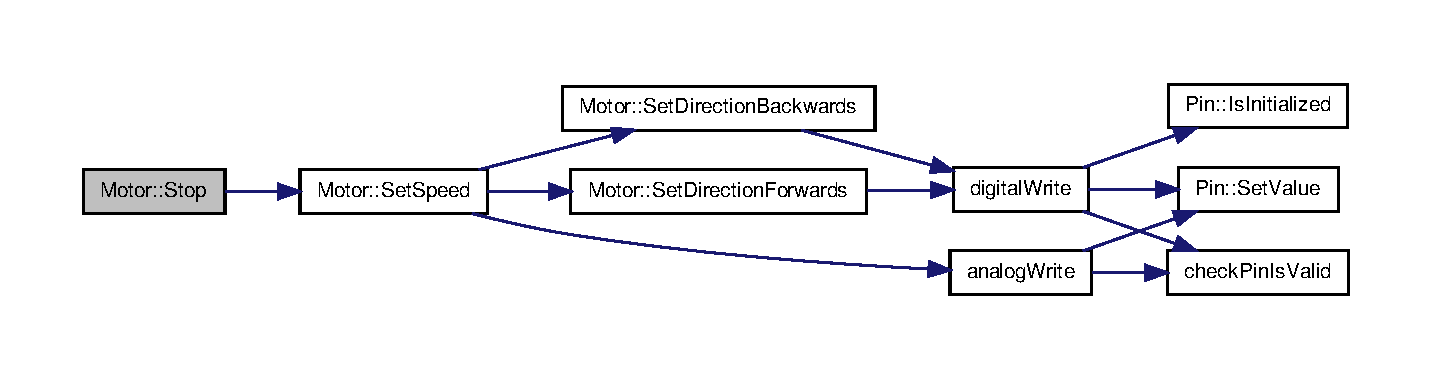
\includegraphics[width=350pt]{class_motor_a8f0fdb6c977ea11e89281c51534850ca_cgraph}
\end{center}
\end{figure}




Here is the caller graph for this function\-:\nopagebreak
\begin{figure}[H]
\begin{center}
\leavevmode
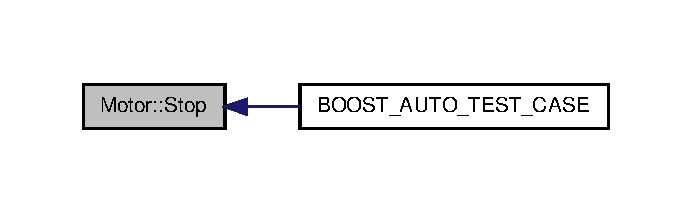
\includegraphics[width=332pt]{class_motor_a8f0fdb6c977ea11e89281c51534850ca_icgraph}
\end{center}
\end{figure}




The documentation for this class was generated from the following files\-:\begin{DoxyCompactItemize}
\item 
lib/motor\-\_\-control/\hyperlink{_motor_8h}{Motor.\-h}\item 
lib/motor\-\_\-control/\hyperlink{_motor_8cpp}{Motor.\-cpp}\end{DoxyCompactItemize}

\hypertarget{class_motor_controller}{\section{Motor\-Controller Class Reference}
\label{class_motor_controller}\index{Motor\-Controller@{Motor\-Controller}}
}


{\ttfamily \#include $<$Motor\-Controller.\-h$>$}



Inheritance diagram for Motor\-Controller\-:
\nopagebreak
\begin{figure}[H]
\begin{center}
\leavevmode
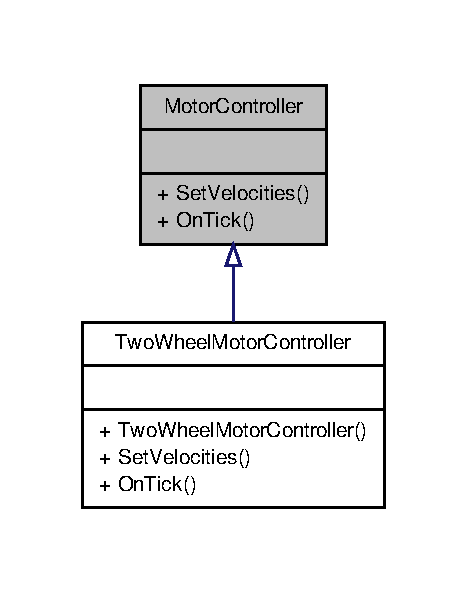
\includegraphics[width=224pt]{class_motor_controller__inherit__graph}
\end{center}
\end{figure}


Collaboration diagram for Motor\-Controller\-:
\nopagebreak
\begin{figure}[H]
\begin{center}
\leavevmode
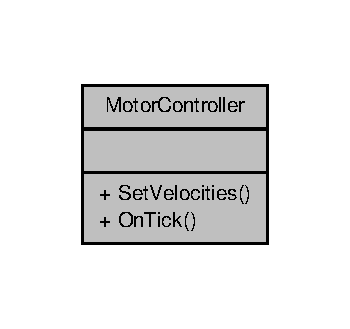
\includegraphics[width=168pt]{class_motor_controller__coll__graph}
\end{center}
\end{figure}
\subsection*{Public Member Functions}
\begin{DoxyCompactItemize}
\item 
virtual void \hyperlink{class_motor_controller_a4ec5e460de5d3767d056aa0ce415049f}{Set\-Velocities} (const int linear\-Velocity, const float angular\-Velocity)=0
\item 
virtual void \hyperlink{class_motor_controller_a699e5bf9a36a2af3914c7fba6b9e7821}{On\-Tick} ()=0
\end{DoxyCompactItemize}


\subsection{Member Function Documentation}
\hypertarget{class_motor_controller_a699e5bf9a36a2af3914c7fba6b9e7821}{\index{Motor\-Controller@{Motor\-Controller}!On\-Tick@{On\-Tick}}
\index{On\-Tick@{On\-Tick}!MotorController@{Motor\-Controller}}
\subsubsection[{On\-Tick}]{\setlength{\rightskip}{0pt plus 5cm}virtual void Motor\-Controller\-::\-On\-Tick (
\begin{DoxyParamCaption}
{}
\end{DoxyParamCaption}
)\hspace{0.3cm}{\ttfamily [pure virtual]}}}\label{class_motor_controller_a699e5bf9a36a2af3914c7fba6b9e7821}


Implemented in \hyperlink{class_two_wheel_motor_controller_a48648184a02f823f44b6b44e84ca9c47}{Two\-Wheel\-Motor\-Controller}.



Here is the caller graph for this function\-:\nopagebreak
\begin{figure}[H]
\begin{center}
\leavevmode
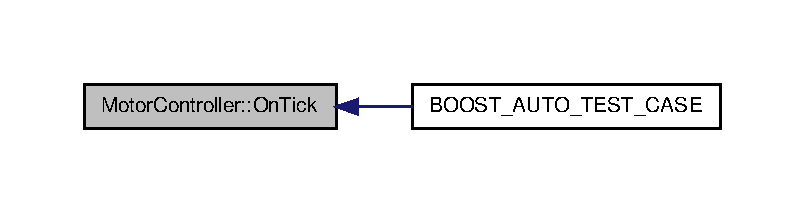
\includegraphics[width=350pt]{class_motor_controller_a699e5bf9a36a2af3914c7fba6b9e7821_icgraph}
\end{center}
\end{figure}


\hypertarget{class_motor_controller_a4ec5e460de5d3767d056aa0ce415049f}{\index{Motor\-Controller@{Motor\-Controller}!Set\-Velocities@{Set\-Velocities}}
\index{Set\-Velocities@{Set\-Velocities}!MotorController@{Motor\-Controller}}
\subsubsection[{Set\-Velocities}]{\setlength{\rightskip}{0pt plus 5cm}virtual void Motor\-Controller\-::\-Set\-Velocities (
\begin{DoxyParamCaption}
\item[{const int}]{linear\-Velocity, }
\item[{const float}]{angular\-Velocity}
\end{DoxyParamCaption}
)\hspace{0.3cm}{\ttfamily [pure virtual]}}}\label{class_motor_controller_a4ec5e460de5d3767d056aa0ce415049f}


Implemented in \hyperlink{class_two_wheel_motor_controller_a43f962d36f8171d7a697a0a011bac98a}{Two\-Wheel\-Motor\-Controller}.



Here is the caller graph for this function\-:\nopagebreak
\begin{figure}[H]
\begin{center}
\leavevmode
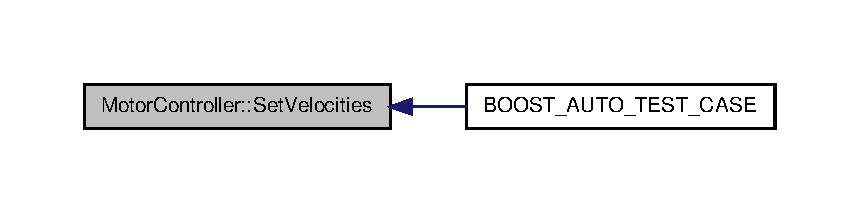
\includegraphics[width=350pt]{class_motor_controller_a4ec5e460de5d3767d056aa0ce415049f_icgraph}
\end{center}
\end{figure}




The documentation for this class was generated from the following file\-:\begin{DoxyCompactItemize}
\item 
lib/motor\-\_\-control/\hyperlink{_motor_controller_8h}{Motor\-Controller.\-h}\end{DoxyCompactItemize}

\hypertarget{struct_no_such_pin_exception}{\section{No\-Such\-Pin\-Exception Struct Reference}
\label{struct_no_such_pin_exception}\index{No\-Such\-Pin\-Exception@{No\-Such\-Pin\-Exception}}
}


{\ttfamily \#include $<$Mock\-W\-Program.\-hpp$>$}



Inheritance diagram for No\-Such\-Pin\-Exception\-:\nopagebreak
\begin{figure}[H]
\begin{center}
\leavevmode
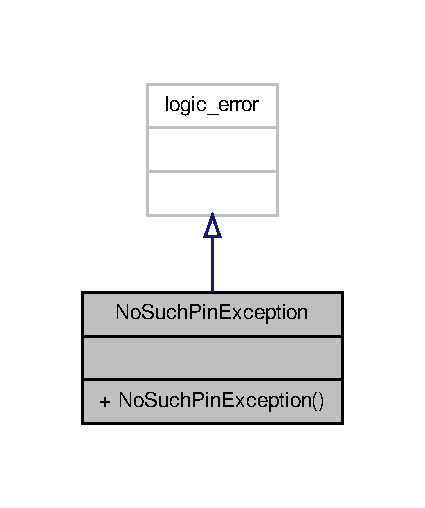
\includegraphics[width=204pt]{struct_no_such_pin_exception__inherit__graph}
\end{center}
\end{figure}


Collaboration diagram for No\-Such\-Pin\-Exception\-:\nopagebreak
\begin{figure}[H]
\begin{center}
\leavevmode
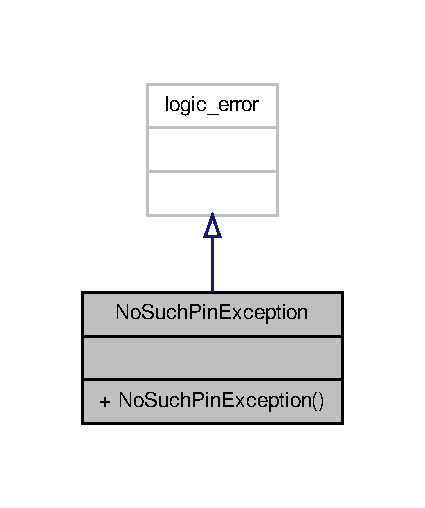
\includegraphics[width=204pt]{struct_no_such_pin_exception__coll__graph}
\end{center}
\end{figure}
\subsection*{Public Member Functions}
\begin{DoxyCompactItemize}
\item 
\hyperlink{struct_no_such_pin_exception_a674ce9ac5719750586c8e76ffef1458b}{No\-Such\-Pin\-Exception} (int pin\-Number)
\end{DoxyCompactItemize}


\subsection{Constructor \& Destructor Documentation}
\hypertarget{struct_no_such_pin_exception_a674ce9ac5719750586c8e76ffef1458b}{\index{No\-Such\-Pin\-Exception@{No\-Such\-Pin\-Exception}!No\-Such\-Pin\-Exception@{No\-Such\-Pin\-Exception}}
\index{No\-Such\-Pin\-Exception@{No\-Such\-Pin\-Exception}!NoSuchPinException@{No\-Such\-Pin\-Exception}}
\subsubsection[{No\-Such\-Pin\-Exception}]{\setlength{\rightskip}{0pt plus 5cm}No\-Such\-Pin\-Exception\-::\-No\-Such\-Pin\-Exception (
\begin{DoxyParamCaption}
\item[{int}]{pin\-Number}
\end{DoxyParamCaption}
)\hspace{0.3cm}{\ttfamily [inline]}}}\label{struct_no_such_pin_exception_a674ce9ac5719750586c8e76ffef1458b}


The documentation for this struct was generated from the following file\-:\begin{DoxyCompactItemize}
\item 
lib/arduino\-\_\-mocks/\hyperlink{_mock_w_program_8hpp}{Mock\-W\-Program.\-hpp}\end{DoxyCompactItemize}

\hypertarget{class_odometry_manager}{\section{Odometry\-Manager Class Reference}
\label{class_odometry_manager}\index{Odometry\-Manager@{Odometry\-Manager}}
}


{\ttfamily \#include $<$Odometry\-Manager.\-h$>$}



Inheritance diagram for Odometry\-Manager\-:
\nopagebreak
\begin{figure}[H]
\begin{center}
\leavevmode
\includegraphics[width=244pt]{class_odometry_manager__inherit__graph}
\end{center}
\end{figure}


Collaboration diagram for Odometry\-Manager\-:
\nopagebreak
\begin{figure}[H]
\begin{center}
\leavevmode
\includegraphics[width=196pt]{class_odometry_manager__coll__graph}
\end{center}
\end{figure}
\subsection*{Public Member Functions}
\begin{DoxyCompactItemize}
\item 
virtual int \hyperlink{class_odometry_manager_a75e7e965b0b224fa747fec22eb0514b7}{Get\-Linear\-Velocity} () const =0
\item 
virtual float \hyperlink{class_odometry_manager_af31cbb9c1f9d1c3b62fd5fe0170e88db}{Get\-Angular\-Velocity} () const =0
\end{DoxyCompactItemize}


\subsection{Member Function Documentation}
\hypertarget{class_odometry_manager_af31cbb9c1f9d1c3b62fd5fe0170e88db}{\index{Odometry\-Manager@{Odometry\-Manager}!Get\-Angular\-Velocity@{Get\-Angular\-Velocity}}
\index{Get\-Angular\-Velocity@{Get\-Angular\-Velocity}!OdometryManager@{Odometry\-Manager}}
\subsubsection[{Get\-Angular\-Velocity}]{\setlength{\rightskip}{0pt plus 5cm}virtual float Odometry\-Manager\-::\-Get\-Angular\-Velocity (
\begin{DoxyParamCaption}
{}
\end{DoxyParamCaption}
) const\hspace{0.3cm}{\ttfamily [pure virtual]}}}\label{class_odometry_manager_af31cbb9c1f9d1c3b62fd5fe0170e88db}


Implemented in \hyperlink{class_two_wheel_odometry_manager_a532a00ad59defba9d54749568cd841ed}{Two\-Wheel\-Odometry\-Manager}.



Here is the caller graph for this function\-:\nopagebreak
\begin{figure}[H]
\begin{center}
\leavevmode
\includegraphics[width=350pt]{class_odometry_manager_af31cbb9c1f9d1c3b62fd5fe0170e88db_icgraph}
\end{center}
\end{figure}


\hypertarget{class_odometry_manager_a75e7e965b0b224fa747fec22eb0514b7}{\index{Odometry\-Manager@{Odometry\-Manager}!Get\-Linear\-Velocity@{Get\-Linear\-Velocity}}
\index{Get\-Linear\-Velocity@{Get\-Linear\-Velocity}!OdometryManager@{Odometry\-Manager}}
\subsubsection[{Get\-Linear\-Velocity}]{\setlength{\rightskip}{0pt plus 5cm}virtual int Odometry\-Manager\-::\-Get\-Linear\-Velocity (
\begin{DoxyParamCaption}
{}
\end{DoxyParamCaption}
) const\hspace{0.3cm}{\ttfamily [pure virtual]}}}\label{class_odometry_manager_a75e7e965b0b224fa747fec22eb0514b7}


Implemented in \hyperlink{class_two_wheel_odometry_manager_a0221669c64b5155424c277dca2e52c2e}{Two\-Wheel\-Odometry\-Manager}.



Here is the caller graph for this function\-:\nopagebreak
\begin{figure}[H]
\begin{center}
\leavevmode
\includegraphics[width=350pt]{class_odometry_manager_a75e7e965b0b224fa747fec22eb0514b7_icgraph}
\end{center}
\end{figure}




The documentation for this class was generated from the following file\-:\begin{DoxyCompactItemize}
\item 
lib/odometry/\hyperlink{_odometry_manager_8h}{Odometry\-Manager.\-h}\end{DoxyCompactItemize}

\hypertarget{class_p_i_d_controlled_motor}{\section{P\-I\-D\-Controlled\-Motor Class Reference}
\label{class_p_i_d_controlled_motor}\index{P\-I\-D\-Controlled\-Motor@{P\-I\-D\-Controlled\-Motor}}
}


{\ttfamily \#include $<$P\-I\-D\-Controlled\-Motor.\-h$>$}



Inheritance diagram for P\-I\-D\-Controlled\-Motor\-:
\nopagebreak
\begin{figure}[H]
\begin{center}
\leavevmode
\includegraphics[width=208pt]{class_p_i_d_controlled_motor__inherit__graph}
\end{center}
\end{figure}


Collaboration diagram for P\-I\-D\-Controlled\-Motor\-:
\nopagebreak
\begin{figure}[H]
\begin{center}
\leavevmode
\includegraphics[width=208pt]{class_p_i_d_controlled_motor__coll__graph}
\end{center}
\end{figure}
\subsection*{Public Member Functions}
\begin{DoxyCompactItemize}
\item 
\hyperlink{class_p_i_d_controlled_motor_a09bc1d7398c15091b44c98b29fc1f073}{P\-I\-D\-Controlled\-Motor} (const unsigned int wheel\-Radius, const \hyperlink{class_motor}{Motor} \&motor, \hyperlink{class_encoder}{Encoder} $\ast$const encoder, const float k\-P, const float k\-I, const float k\-D)
\item 
\hyperlink{class_p_i_d_controlled_motor_a6cb0559e4413a30318ba576d59cd3fff}{P\-I\-D\-Controlled\-Motor} (const unsigned int wheel\-Radius, const \hyperlink{class_motor}{Motor} \&motor, \hyperlink{class_encoder}{Encoder} $\ast$const encoder)
\item 
void \hyperlink{class_p_i_d_controlled_motor_a045762a3ef93b7b25a6339cda504e4e5}{Set\-Velocity} (const float velocity)
\item 
void \hyperlink{class_p_i_d_controlled_motor_a7ab5288c0d1df6540475634c9a150df2}{Update} ()
\end{DoxyCompactItemize}


\subsection{Constructor \& Destructor Documentation}
\hypertarget{class_p_i_d_controlled_motor_a09bc1d7398c15091b44c98b29fc1f073}{\index{P\-I\-D\-Controlled\-Motor@{P\-I\-D\-Controlled\-Motor}!P\-I\-D\-Controlled\-Motor@{P\-I\-D\-Controlled\-Motor}}
\index{P\-I\-D\-Controlled\-Motor@{P\-I\-D\-Controlled\-Motor}!PIDControlledMotor@{P\-I\-D\-Controlled\-Motor}}
\subsubsection[{P\-I\-D\-Controlled\-Motor}]{\setlength{\rightskip}{0pt plus 5cm}P\-I\-D\-Controlled\-Motor\-::\-P\-I\-D\-Controlled\-Motor (
\begin{DoxyParamCaption}
\item[{const unsigned int}]{wheel\-Radius, }
\item[{const {\bf Motor} \&}]{motor, }
\item[{{\bf Encoder} $\ast$const}]{encoder, }
\item[{const float}]{k\-P, }
\item[{const float}]{k\-I, }
\item[{const float}]{k\-D}
\end{DoxyParamCaption}
)}}\label{class_p_i_d_controlled_motor_a09bc1d7398c15091b44c98b29fc1f073}
\hypertarget{class_p_i_d_controlled_motor_a6cb0559e4413a30318ba576d59cd3fff}{\index{P\-I\-D\-Controlled\-Motor@{P\-I\-D\-Controlled\-Motor}!P\-I\-D\-Controlled\-Motor@{P\-I\-D\-Controlled\-Motor}}
\index{P\-I\-D\-Controlled\-Motor@{P\-I\-D\-Controlled\-Motor}!PIDControlledMotor@{P\-I\-D\-Controlled\-Motor}}
\subsubsection[{P\-I\-D\-Controlled\-Motor}]{\setlength{\rightskip}{0pt plus 5cm}P\-I\-D\-Controlled\-Motor\-::\-P\-I\-D\-Controlled\-Motor (
\begin{DoxyParamCaption}
\item[{const unsigned int}]{wheel\-Radius, }
\item[{const {\bf Motor} \&}]{motor, }
\item[{{\bf Encoder} $\ast$const}]{encoder}
\end{DoxyParamCaption}
)}}\label{class_p_i_d_controlled_motor_a6cb0559e4413a30318ba576d59cd3fff}


\subsection{Member Function Documentation}
\hypertarget{class_p_i_d_controlled_motor_a045762a3ef93b7b25a6339cda504e4e5}{\index{P\-I\-D\-Controlled\-Motor@{P\-I\-D\-Controlled\-Motor}!Set\-Velocity@{Set\-Velocity}}
\index{Set\-Velocity@{Set\-Velocity}!PIDControlledMotor@{P\-I\-D\-Controlled\-Motor}}
\subsubsection[{Set\-Velocity}]{\setlength{\rightskip}{0pt plus 5cm}void P\-I\-D\-Controlled\-Motor\-::\-Set\-Velocity (
\begin{DoxyParamCaption}
\item[{const float}]{velocity}
\end{DoxyParamCaption}
)\hspace{0.3cm}{\ttfamily [inline]}, {\ttfamily [virtual]}}}\label{class_p_i_d_controlled_motor_a045762a3ef93b7b25a6339cda504e4e5}


Implements \hyperlink{class_feedback_controlled_motor_a533fbeddd7edc7035d5d374e9f4ad118}{Feedback\-Controlled\-Motor}.



Here is the caller graph for this function\-:\nopagebreak
\begin{figure}[H]
\begin{center}
\leavevmode
\includegraphics[width=350pt]{class_p_i_d_controlled_motor_a045762a3ef93b7b25a6339cda504e4e5_icgraph}
\end{center}
\end{figure}


\hypertarget{class_p_i_d_controlled_motor_a7ab5288c0d1df6540475634c9a150df2}{\index{P\-I\-D\-Controlled\-Motor@{P\-I\-D\-Controlled\-Motor}!Update@{Update}}
\index{Update@{Update}!PIDControlledMotor@{P\-I\-D\-Controlled\-Motor}}
\subsubsection[{Update}]{\setlength{\rightskip}{0pt plus 5cm}void P\-I\-D\-Controlled\-Motor\-::\-Update (
\begin{DoxyParamCaption}
{}
\end{DoxyParamCaption}
)\hspace{0.3cm}{\ttfamily [virtual]}}}\label{class_p_i_d_controlled_motor_a7ab5288c0d1df6540475634c9a150df2}


Implements \hyperlink{class_feedback_controlled_motor_a54668f85a8dadb66971ee8c8a76be802}{Feedback\-Controlled\-Motor}.



Here is the call graph for this function\-:
\nopagebreak
\begin{figure}[H]
\begin{center}
\leavevmode
\includegraphics[width=350pt]{class_p_i_d_controlled_motor_a7ab5288c0d1df6540475634c9a150df2_cgraph}
\end{center}
\end{figure}




Here is the caller graph for this function\-:\nopagebreak
\begin{figure}[H]
\begin{center}
\leavevmode
\includegraphics[width=350pt]{class_p_i_d_controlled_motor_a7ab5288c0d1df6540475634c9a150df2_icgraph}
\end{center}
\end{figure}




The documentation for this class was generated from the following files\-:\begin{DoxyCompactItemize}
\item 
lib/motor\-\_\-control/\hyperlink{_p_i_d_controlled_motor_8h}{P\-I\-D\-Controlled\-Motor.\-h}\item 
lib/motor\-\_\-control/\hyperlink{_p_i_d_controlled_motor_8cpp}{P\-I\-D\-Controlled\-Motor.\-cpp}\end{DoxyCompactItemize}

\hypertarget{class_pin}{\section{Pin Class Reference}
\label{class_pin}\index{Pin@{Pin}}
}


{\ttfamily \#include $<$Mock\-W\-Program.\-hpp$>$}



Collaboration diagram for Pin\-:\nopagebreak
\begin{figure}[H]
\begin{center}
\leavevmode
\includegraphics[width=160pt]{class_pin__coll__graph}
\end{center}
\end{figure}
\subsection*{Public Member Functions}
\begin{DoxyCompactItemize}
\item 
\hyperlink{class_pin_aaf3d92065cd9b9de91f01164bec418ea}{Pin} ()
\item 
void \hyperlink{class_pin_a818cf19e4b42d2777326c52a56ae4ea9}{Set\-Mode} (uint8\-\_\-t io)
\item 
void \hyperlink{class_pin_adc8d5cd4aeca8cce795e85b3fe1d9a20}{Set\-Value} (uint8\-\_\-t new\-Value)
\item 
void \hyperlink{class_pin_a63ccf03925afd8dc45e5ad5aabc5342a}{Reset} ()
\item 
uint8\-\_\-t \hyperlink{class_pin_a9c39b8c7ef953b40043e97fecb8b35dd}{Get\-Value} ()
\item 
uint8\-\_\-t \hyperlink{class_pin_aae8f8b8ed2e268bfd63e7c06e1d845fd}{Get\-Mode} ()
\item 
bool \hyperlink{class_pin_a56f7dc430291a53b5c08df50c8f43f9a}{Is\-Initialized} ()
\end{DoxyCompactItemize}


\subsection{Constructor \& Destructor Documentation}
\hypertarget{class_pin_aaf3d92065cd9b9de91f01164bec418ea}{\index{Pin@{Pin}!Pin@{Pin}}
\index{Pin@{Pin}!Pin@{Pin}}
\subsubsection[{Pin}]{\setlength{\rightskip}{0pt plus 5cm}Pin\-::\-Pin (
\begin{DoxyParamCaption}
{}
\end{DoxyParamCaption}
)}}\label{class_pin_aaf3d92065cd9b9de91f01164bec418ea}


\subsection{Member Function Documentation}
\hypertarget{class_pin_aae8f8b8ed2e268bfd63e7c06e1d845fd}{\index{Pin@{Pin}!Get\-Mode@{Get\-Mode}}
\index{Get\-Mode@{Get\-Mode}!Pin@{Pin}}
\subsubsection[{Get\-Mode}]{\setlength{\rightskip}{0pt plus 5cm}uint8\-\_\-t Pin\-::\-Get\-Mode (
\begin{DoxyParamCaption}
{}
\end{DoxyParamCaption}
)\hspace{0.3cm}{\ttfamily [inline]}}}\label{class_pin_aae8f8b8ed2e268bfd63e7c06e1d845fd}


Here is the caller graph for this function\-:
\nopagebreak
\begin{figure}[H]
\begin{center}
\leavevmode
\includegraphics[width=260pt]{class_pin_aae8f8b8ed2e268bfd63e7c06e1d845fd_icgraph}
\end{center}
\end{figure}


\hypertarget{class_pin_a9c39b8c7ef953b40043e97fecb8b35dd}{\index{Pin@{Pin}!Get\-Value@{Get\-Value}}
\index{Get\-Value@{Get\-Value}!Pin@{Pin}}
\subsubsection[{Get\-Value}]{\setlength{\rightskip}{0pt plus 5cm}uint8\-\_\-t Pin\-::\-Get\-Value (
\begin{DoxyParamCaption}
{}
\end{DoxyParamCaption}
)\hspace{0.3cm}{\ttfamily [inline]}}}\label{class_pin_a9c39b8c7ef953b40043e97fecb8b35dd}


Here is the caller graph for this function\-:
\nopagebreak
\begin{figure}[H]
\begin{center}
\leavevmode
\includegraphics[width=342pt]{class_pin_a9c39b8c7ef953b40043e97fecb8b35dd_icgraph}
\end{center}
\end{figure}


\hypertarget{class_pin_a56f7dc430291a53b5c08df50c8f43f9a}{\index{Pin@{Pin}!Is\-Initialized@{Is\-Initialized}}
\index{Is\-Initialized@{Is\-Initialized}!Pin@{Pin}}
\subsubsection[{Is\-Initialized}]{\setlength{\rightskip}{0pt plus 5cm}bool Pin\-::\-Is\-Initialized (
\begin{DoxyParamCaption}
{}
\end{DoxyParamCaption}
)\hspace{0.3cm}{\ttfamily [inline]}}}\label{class_pin_a56f7dc430291a53b5c08df50c8f43f9a}


Here is the caller graph for this function\-:
\nopagebreak
\begin{figure}[H]
\begin{center}
\leavevmode
\includegraphics[width=350pt]{class_pin_a56f7dc430291a53b5c08df50c8f43f9a_icgraph}
\end{center}
\end{figure}


\hypertarget{class_pin_a63ccf03925afd8dc45e5ad5aabc5342a}{\index{Pin@{Pin}!Reset@{Reset}}
\index{Reset@{Reset}!Pin@{Pin}}
\subsubsection[{Reset}]{\setlength{\rightskip}{0pt plus 5cm}void Pin\-::\-Reset (
\begin{DoxyParamCaption}
{}
\end{DoxyParamCaption}
)}}\label{class_pin_a63ccf03925afd8dc45e5ad5aabc5342a}
\hypertarget{class_pin_a818cf19e4b42d2777326c52a56ae4ea9}{\index{Pin@{Pin}!Set\-Mode@{Set\-Mode}}
\index{Set\-Mode@{Set\-Mode}!Pin@{Pin}}
\subsubsection[{Set\-Mode}]{\setlength{\rightskip}{0pt plus 5cm}void Pin\-::\-Set\-Mode (
\begin{DoxyParamCaption}
\item[{uint8\-\_\-t}]{io}
\end{DoxyParamCaption}
)}}\label{class_pin_a818cf19e4b42d2777326c52a56ae4ea9}


Here is the caller graph for this function\-:
\nopagebreak
\begin{figure}[H]
\begin{center}
\leavevmode
\includegraphics[width=350pt]{class_pin_a818cf19e4b42d2777326c52a56ae4ea9_icgraph}
\end{center}
\end{figure}


\hypertarget{class_pin_adc8d5cd4aeca8cce795e85b3fe1d9a20}{\index{Pin@{Pin}!Set\-Value@{Set\-Value}}
\index{Set\-Value@{Set\-Value}!Pin@{Pin}}
\subsubsection[{Set\-Value}]{\setlength{\rightskip}{0pt plus 5cm}void Pin\-::\-Set\-Value (
\begin{DoxyParamCaption}
\item[{uint8\-\_\-t}]{new\-Value}
\end{DoxyParamCaption}
)}}\label{class_pin_adc8d5cd4aeca8cce795e85b3fe1d9a20}


Here is the caller graph for this function\-:
\nopagebreak
\begin{figure}[H]
\begin{center}
\leavevmode
\includegraphics[width=350pt]{class_pin_adc8d5cd4aeca8cce795e85b3fe1d9a20_icgraph}
\end{center}
\end{figure}




The documentation for this class was generated from the following files\-:\begin{DoxyCompactItemize}
\item 
lib/arduino\-\_\-mocks/\hyperlink{_mock_w_program_8hpp}{Mock\-W\-Program.\-hpp}\item 
lib/arduino\-\_\-mocks/\hyperlink{_mock_w_program_8cpp}{Mock\-W\-Program.\-cpp}\end{DoxyCompactItemize}

\hypertarget{class_rotary_encoder}{\section{Rotary\-Encoder$<$ interrupt\-Pin $>$ Class Template Reference}
\label{class_rotary_encoder}\index{Rotary\-Encoder$<$ interrupt\-Pin $>$@{Rotary\-Encoder$<$ interrupt\-Pin $>$}}
}


{\ttfamily \#include $<$Rotary\-Encoder.\-h$>$}



Inheritance diagram for Rotary\-Encoder$<$ interrupt\-Pin $>$\-:
\nopagebreak
\begin{figure}[H]
\begin{center}
\leavevmode
\includegraphics[width=210pt]{class_rotary_encoder__inherit__graph}
\end{center}
\end{figure}


Collaboration diagram for Rotary\-Encoder$<$ interrupt\-Pin $>$\-:
\nopagebreak
\begin{figure}[H]
\begin{center}
\leavevmode
\includegraphics[width=210pt]{class_rotary_encoder__coll__graph}
\end{center}
\end{figure}
\subsection*{Public Member Functions}
\begin{DoxyCompactItemize}
\item 
\hyperlink{class_rotary_encoder_a9c59eaec8c45def05d639a22324d60c5}{Rotary\-Encoder} (uint8\-\_\-t encoder\-Input\-A, uint8\-\_\-t encoder\-Input\-B, float ratio)
\item 
virtual float \hyperlink{class_rotary_encoder_a7ec02990f0ffb7bb62a3a76f0fd64ade}{Revolutions\-Per\-Second} ()
\item 
virtual float \hyperlink{class_rotary_encoder_a3dea9166b76dad99ee708c4ff1fde9f8}{Get\-Frequency} ()
\item 
virtual \hyperlink{class_encoder_aa7c4648a7ebc9e651c25c2d450a58213}{Direction} \hyperlink{class_rotary_encoder_aa62141a77e01d0d44706f3b421e3ae25}{Get\-Direction} () const 
\end{DoxyCompactItemize}
\subsection*{Static Public Member Functions}
\begin{DoxyCompactItemize}
\item 
static void \hyperlink{class_rotary_encoder_ad884c21ff3f1c2e382bc3a72596e1ec4}{Handler} ()
\end{DoxyCompactItemize}
\subsection*{Static Public Attributes}
\begin{DoxyCompactItemize}
\item 
static constexpr int \hyperlink{class_rotary_encoder_a97a8bdc99c6ce9ca44d4a668d6355a7c}{Rotary\-Encoder\-Matrix} \mbox{[}$\,$\mbox{]}
\end{DoxyCompactItemize}
\subsection*{Additional Inherited Members}


\subsection{Constructor \& Destructor Documentation}
\hypertarget{class_rotary_encoder_a9c59eaec8c45def05d639a22324d60c5}{\index{Rotary\-Encoder@{Rotary\-Encoder}!Rotary\-Encoder@{Rotary\-Encoder}}
\index{Rotary\-Encoder@{Rotary\-Encoder}!RotaryEncoder@{Rotary\-Encoder}}
\subsubsection[{Rotary\-Encoder}]{\setlength{\rightskip}{0pt plus 5cm}template$<$Wheel side$>$ {\bf Rotary\-Encoder}$<$ side $>$\-::{\bf Rotary\-Encoder} (
\begin{DoxyParamCaption}
\item[{uint8\-\_\-t}]{encoder\-Input\-A, }
\item[{uint8\-\_\-t}]{encoder\-Input\-B, }
\item[{float}]{ratio}
\end{DoxyParamCaption}
)}}\label{class_rotary_encoder_a9c59eaec8c45def05d639a22324d60c5}


Here is the call graph for this function\-:
\nopagebreak
\begin{figure}[H]
\begin{center}
\leavevmode
\includegraphics[width=350pt]{class_rotary_encoder_a9c59eaec8c45def05d639a22324d60c5_cgraph}
\end{center}
\end{figure}




\subsection{Member Function Documentation}
\hypertarget{class_rotary_encoder_aa62141a77e01d0d44706f3b421e3ae25}{\index{Rotary\-Encoder@{Rotary\-Encoder}!Get\-Direction@{Get\-Direction}}
\index{Get\-Direction@{Get\-Direction}!RotaryEncoder@{Rotary\-Encoder}}
\subsubsection[{Get\-Direction}]{\setlength{\rightskip}{0pt plus 5cm}template$<$Wheel interrupt\-Pin$>$ virtual {\bf Direction} {\bf Rotary\-Encoder}$<$ interrupt\-Pin $>$\-::Get\-Direction (
\begin{DoxyParamCaption}
{}
\end{DoxyParamCaption}
) const\hspace{0.3cm}{\ttfamily [inline]}, {\ttfamily [virtual]}}}\label{class_rotary_encoder_aa62141a77e01d0d44706f3b421e3ae25}


Implements \hyperlink{class_encoder_ab4faff630f313bc0e5b8718df3175fe1}{Encoder}.



Here is the caller graph for this function\-:\nopagebreak
\begin{figure}[H]
\begin{center}
\leavevmode
\includegraphics[width=350pt]{class_rotary_encoder_aa62141a77e01d0d44706f3b421e3ae25_icgraph}
\end{center}
\end{figure}


\hypertarget{class_rotary_encoder_a3dea9166b76dad99ee708c4ff1fde9f8}{\index{Rotary\-Encoder@{Rotary\-Encoder}!Get\-Frequency@{Get\-Frequency}}
\index{Get\-Frequency@{Get\-Frequency}!RotaryEncoder@{Rotary\-Encoder}}
\subsubsection[{Get\-Frequency}]{\setlength{\rightskip}{0pt plus 5cm}template$<$Wheel side$>$ float {\bf Rotary\-Encoder}$<$ side $>$\-::Get\-Frequency (
\begin{DoxyParamCaption}
{}
\end{DoxyParamCaption}
)\hspace{0.3cm}{\ttfamily [virtual]}}}\label{class_rotary_encoder_a3dea9166b76dad99ee708c4ff1fde9f8}


Implements \hyperlink{class_encoder_ab52587693b386731fcdef289e590fc40}{Encoder}.



Here is the call graph for this function\-:
\nopagebreak
\begin{figure}[H]
\begin{center}
\leavevmode
\includegraphics[width=312pt]{class_rotary_encoder_a3dea9166b76dad99ee708c4ff1fde9f8_cgraph}
\end{center}
\end{figure}




Here is the caller graph for this function\-:\nopagebreak
\begin{figure}[H]
\begin{center}
\leavevmode
\includegraphics[width=350pt]{class_rotary_encoder_a3dea9166b76dad99ee708c4ff1fde9f8_icgraph}
\end{center}
\end{figure}


\hypertarget{class_rotary_encoder_ad884c21ff3f1c2e382bc3a72596e1ec4}{\index{Rotary\-Encoder@{Rotary\-Encoder}!Handler@{Handler}}
\index{Handler@{Handler}!RotaryEncoder@{Rotary\-Encoder}}
\subsubsection[{Handler}]{\setlength{\rightskip}{0pt plus 5cm}template$<$Wheel side$>$ void {\bf Rotary\-Encoder}$<$ side $>$\-::Handler (
\begin{DoxyParamCaption}
{}
\end{DoxyParamCaption}
)\hspace{0.3cm}{\ttfamily [static]}}}\label{class_rotary_encoder_ad884c21ff3f1c2e382bc3a72596e1ec4}


Here is the caller graph for this function\-:\nopagebreak
\begin{figure}[H]
\begin{center}
\leavevmode
\includegraphics[width=350pt]{class_rotary_encoder_ad884c21ff3f1c2e382bc3a72596e1ec4_icgraph}
\end{center}
\end{figure}


\hypertarget{class_rotary_encoder_a7ec02990f0ffb7bb62a3a76f0fd64ade}{\index{Rotary\-Encoder@{Rotary\-Encoder}!Revolutions\-Per\-Second@{Revolutions\-Per\-Second}}
\index{Revolutions\-Per\-Second@{Revolutions\-Per\-Second}!RotaryEncoder@{Rotary\-Encoder}}
\subsubsection[{Revolutions\-Per\-Second}]{\setlength{\rightskip}{0pt plus 5cm}template$<$Wheel side$>$ float {\bf Rotary\-Encoder}$<$ side $>$\-::Revolutions\-Per\-Second (
\begin{DoxyParamCaption}
{}
\end{DoxyParamCaption}
)\hspace{0.3cm}{\ttfamily [virtual]}}}\label{class_rotary_encoder_a7ec02990f0ffb7bb62a3a76f0fd64ade}


Implements \hyperlink{class_encoder_a758adfad11078f8dec0ca672929a4189}{Encoder}.



Here is the caller graph for this function\-:\nopagebreak
\begin{figure}[H]
\begin{center}
\leavevmode
\includegraphics[width=350pt]{class_rotary_encoder_a7ec02990f0ffb7bb62a3a76f0fd64ade_icgraph}
\end{center}
\end{figure}




\subsection{Member Data Documentation}
\hypertarget{class_rotary_encoder_a97a8bdc99c6ce9ca44d4a668d6355a7c}{\index{Rotary\-Encoder@{Rotary\-Encoder}!Rotary\-Encoder\-Matrix@{Rotary\-Encoder\-Matrix}}
\index{Rotary\-Encoder\-Matrix@{Rotary\-Encoder\-Matrix}!RotaryEncoder@{Rotary\-Encoder}}
\subsubsection[{Rotary\-Encoder\-Matrix}]{\setlength{\rightskip}{0pt plus 5cm}template$<$Wheel interrupt\-Pin$>$ constexpr int {\bf Rotary\-Encoder}$<$ side $>$\-::Rotary\-Encoder\-Matrix\hspace{0.3cm}{\ttfamily [static]}}}\label{class_rotary_encoder_a97a8bdc99c6ce9ca44d4a668d6355a7c}
{\bfseries Initial value\-:}
\begin{DoxyCode}
= \{0,\hyperlink{class_encoder_aa7c4648a7ebc9e651c25c2d450a58213a9fb277421175dd4894688e30dd757253}{BACKWARDS},\hyperlink{class_encoder_aa7c4648a7ebc9e651c25c2d450a58213a75ee06096317d25b47119647e33622cf}{FORWARDS},2, 
                                                  \hyperlink{class_encoder_aa7c4648a7ebc9e651c25c2d450a58213a75ee06096317d25b47119647e33622cf}{FORWARDS},0,2,\hyperlink{class_encoder_aa7c4648a7ebc9e651c25c2d450a58213a9fb277421175dd4894688e30dd757253}{BACKWARDS}, 
                                                  \hyperlink{class_encoder_aa7c4648a7ebc9e651c25c2d450a58213a9fb277421175dd4894688e30dd757253}{BACKWARDS},2,0,
      \hyperlink{class_encoder_aa7c4648a7ebc9e651c25c2d450a58213a75ee06096317d25b47119647e33622cf}{FORWARDS}, 
                                                  2,\hyperlink{class_encoder_aa7c4648a7ebc9e651c25c2d450a58213a75ee06096317d25b47119647e33622cf}{FORWARDS}, \hyperlink{class_encoder_aa7c4648a7ebc9e651c25c2d450a58213a9fb277421175dd4894688e30dd757253}{BACKWARDS},0\}
\end{DoxyCode}


The documentation for this class was generated from the following files\-:\begin{DoxyCompactItemize}
\item 
lib/odometry/\hyperlink{_rotary_encoder_8h}{Rotary\-Encoder.\-h}\item 
lib/odometry/\hyperlink{_rotary_encoder_8hpp}{Rotary\-Encoder.\-hpp}\end{DoxyCompactItemize}

\hypertarget{class_two_wheel_motor_controller}{\section{Two\-Wheel\-Motor\-Controller Class Reference}
\label{class_two_wheel_motor_controller}\index{Two\-Wheel\-Motor\-Controller@{Two\-Wheel\-Motor\-Controller}}
}


{\ttfamily \#include $<$Two\-Wheel\-Motor\-Controller.\-h$>$}



Inheritance diagram for Two\-Wheel\-Motor\-Controller\-:
\nopagebreak
\begin{figure}[H]
\begin{center}
\leavevmode
\includegraphics[width=224pt]{class_two_wheel_motor_controller__inherit__graph}
\end{center}
\end{figure}


Collaboration diagram for Two\-Wheel\-Motor\-Controller\-:
\nopagebreak
\begin{figure}[H]
\begin{center}
\leavevmode
\includegraphics[width=224pt]{class_two_wheel_motor_controller__coll__graph}
\end{center}
\end{figure}
\subsection*{Public Member Functions}
\begin{DoxyCompactItemize}
\item 
\hyperlink{class_two_wheel_motor_controller_a15d394ce52b9253e0e34286b6ea7b141}{Two\-Wheel\-Motor\-Controller} (\hyperlink{class_feedback_controlled_motor}{Feedback\-Controlled\-Motor} $\ast$const left, \hyperlink{class_feedback_controlled_motor}{Feedback\-Controlled\-Motor} $\ast$const right, const int width)
\item 
void \hyperlink{class_two_wheel_motor_controller_a43f962d36f8171d7a697a0a011bac98a}{Set\-Velocities} (const int linear\-Velocity, const float angular\-Velocity)
\item 
void \hyperlink{class_two_wheel_motor_controller_a48648184a02f823f44b6b44e84ca9c47}{On\-Tick} ()
\end{DoxyCompactItemize}


\subsection{Constructor \& Destructor Documentation}
\hypertarget{class_two_wheel_motor_controller_a15d394ce52b9253e0e34286b6ea7b141}{\index{Two\-Wheel\-Motor\-Controller@{Two\-Wheel\-Motor\-Controller}!Two\-Wheel\-Motor\-Controller@{Two\-Wheel\-Motor\-Controller}}
\index{Two\-Wheel\-Motor\-Controller@{Two\-Wheel\-Motor\-Controller}!TwoWheelMotorController@{Two\-Wheel\-Motor\-Controller}}
\subsubsection[{Two\-Wheel\-Motor\-Controller}]{\setlength{\rightskip}{0pt plus 5cm}Two\-Wheel\-Motor\-Controller\-::\-Two\-Wheel\-Motor\-Controller (
\begin{DoxyParamCaption}
\item[{{\bf Feedback\-Controlled\-Motor} $\ast$const}]{left, }
\item[{{\bf Feedback\-Controlled\-Motor} $\ast$const}]{right, }
\item[{const int}]{width}
\end{DoxyParamCaption}
)}}\label{class_two_wheel_motor_controller_a15d394ce52b9253e0e34286b6ea7b141}


\subsection{Member Function Documentation}
\hypertarget{class_two_wheel_motor_controller_a48648184a02f823f44b6b44e84ca9c47}{\index{Two\-Wheel\-Motor\-Controller@{Two\-Wheel\-Motor\-Controller}!On\-Tick@{On\-Tick}}
\index{On\-Tick@{On\-Tick}!TwoWheelMotorController@{Two\-Wheel\-Motor\-Controller}}
\subsubsection[{On\-Tick}]{\setlength{\rightskip}{0pt plus 5cm}void Two\-Wheel\-Motor\-Controller\-::\-On\-Tick (
\begin{DoxyParamCaption}
{}
\end{DoxyParamCaption}
)\hspace{0.3cm}{\ttfamily [virtual]}}}\label{class_two_wheel_motor_controller_a48648184a02f823f44b6b44e84ca9c47}


Implements \hyperlink{class_motor_controller_a699e5bf9a36a2af3914c7fba6b9e7821}{Motor\-Controller}.



Here is the call graph for this function\-:\nopagebreak
\begin{figure}[H]
\begin{center}
\leavevmode
\includegraphics[width=350pt]{class_two_wheel_motor_controller_a48648184a02f823f44b6b44e84ca9c47_cgraph}
\end{center}
\end{figure}




Here is the caller graph for this function\-:\nopagebreak
\begin{figure}[H]
\begin{center}
\leavevmode
\includegraphics[width=350pt]{class_two_wheel_motor_controller_a48648184a02f823f44b6b44e84ca9c47_icgraph}
\end{center}
\end{figure}


\hypertarget{class_two_wheel_motor_controller_a43f962d36f8171d7a697a0a011bac98a}{\index{Two\-Wheel\-Motor\-Controller@{Two\-Wheel\-Motor\-Controller}!Set\-Velocities@{Set\-Velocities}}
\index{Set\-Velocities@{Set\-Velocities}!TwoWheelMotorController@{Two\-Wheel\-Motor\-Controller}}
\subsubsection[{Set\-Velocities}]{\setlength{\rightskip}{0pt plus 5cm}void Two\-Wheel\-Motor\-Controller\-::\-Set\-Velocities (
\begin{DoxyParamCaption}
\item[{const int}]{linear\-Velocity, }
\item[{const float}]{angular\-Velocity}
\end{DoxyParamCaption}
)\hspace{0.3cm}{\ttfamily [virtual]}}}\label{class_two_wheel_motor_controller_a43f962d36f8171d7a697a0a011bac98a}


Implements \hyperlink{class_motor_controller_a4ec5e460de5d3767d056aa0ce415049f}{Motor\-Controller}.



Here is the caller graph for this function\-:\nopagebreak
\begin{figure}[H]
\begin{center}
\leavevmode
\includegraphics[width=350pt]{class_two_wheel_motor_controller_a43f962d36f8171d7a697a0a011bac98a_icgraph}
\end{center}
\end{figure}




The documentation for this class was generated from the following files\-:\begin{DoxyCompactItemize}
\item 
lib/motor\-\_\-control/\hyperlink{_two_wheel_motor_controller_8h}{Two\-Wheel\-Motor\-Controller.\-h}\item 
lib/motor\-\_\-control/\hyperlink{_two_wheel_motor_controller_8cpp}{Two\-Wheel\-Motor\-Controller.\-cpp}\end{DoxyCompactItemize}

\hypertarget{class_two_wheel_odometry_manager}{\section{Two\-Wheel\-Odometry\-Manager Class Reference}
\label{class_two_wheel_odometry_manager}\index{Two\-Wheel\-Odometry\-Manager@{Two\-Wheel\-Odometry\-Manager}}
}


{\ttfamily \#include $<$Two\-Wheel\-Odometry\-Manager.\-h$>$}



Inheritance diagram for Two\-Wheel\-Odometry\-Manager\-:
\nopagebreak
\begin{figure}[H]
\begin{center}
\leavevmode
\includegraphics[width=244pt]{class_two_wheel_odometry_manager__inherit__graph}
\end{center}
\end{figure}


Collaboration diagram for Two\-Wheel\-Odometry\-Manager\-:
\nopagebreak
\begin{figure}[H]
\begin{center}
\leavevmode
\includegraphics[width=244pt]{class_two_wheel_odometry_manager__coll__graph}
\end{center}
\end{figure}
\subsection*{Public Member Functions}
\begin{DoxyCompactItemize}
\item 
\hyperlink{class_two_wheel_odometry_manager_a8ac5ef96d7753f0022803b0580591ca1}{Two\-Wheel\-Odometry\-Manager} (int width, int wheel\-Radius, \hyperlink{class_encoder}{Encoder} $\ast$left\-Encoder, \hyperlink{class_encoder}{Encoder} $\ast$right\-Encoder)
\item 
\hyperlink{class_two_wheel_odometry_manager_ab6a596af05b4606d60fb169b82710e04}{$\sim$\-Two\-Wheel\-Odometry\-Manager} ()
\item 
virtual int \hyperlink{class_two_wheel_odometry_manager_a0221669c64b5155424c277dca2e52c2e}{Get\-Linear\-Velocity} () const 
\item 
virtual float \hyperlink{class_two_wheel_odometry_manager_a532a00ad59defba9d54749568cd841ed}{Get\-Angular\-Velocity} () const 
\end{DoxyCompactItemize}


\subsection{Constructor \& Destructor Documentation}
\hypertarget{class_two_wheel_odometry_manager_a8ac5ef96d7753f0022803b0580591ca1}{\index{Two\-Wheel\-Odometry\-Manager@{Two\-Wheel\-Odometry\-Manager}!Two\-Wheel\-Odometry\-Manager@{Two\-Wheel\-Odometry\-Manager}}
\index{Two\-Wheel\-Odometry\-Manager@{Two\-Wheel\-Odometry\-Manager}!TwoWheelOdometryManager@{Two\-Wheel\-Odometry\-Manager}}
\subsubsection[{Two\-Wheel\-Odometry\-Manager}]{\setlength{\rightskip}{0pt plus 5cm}Two\-Wheel\-Odometry\-Manager\-::\-Two\-Wheel\-Odometry\-Manager (
\begin{DoxyParamCaption}
\item[{int}]{width, }
\item[{int}]{wheel\-Radius, }
\item[{{\bf Encoder} $\ast$}]{left\-Encoder, }
\item[{{\bf Encoder} $\ast$}]{right\-Encoder}
\end{DoxyParamCaption}
)}}\label{class_two_wheel_odometry_manager_a8ac5ef96d7753f0022803b0580591ca1}
\hypertarget{class_two_wheel_odometry_manager_ab6a596af05b4606d60fb169b82710e04}{\index{Two\-Wheel\-Odometry\-Manager@{Two\-Wheel\-Odometry\-Manager}!$\sim$\-Two\-Wheel\-Odometry\-Manager@{$\sim$\-Two\-Wheel\-Odometry\-Manager}}
\index{$\sim$\-Two\-Wheel\-Odometry\-Manager@{$\sim$\-Two\-Wheel\-Odometry\-Manager}!TwoWheelOdometryManager@{Two\-Wheel\-Odometry\-Manager}}
\subsubsection[{$\sim$\-Two\-Wheel\-Odometry\-Manager}]{\setlength{\rightskip}{0pt plus 5cm}Two\-Wheel\-Odometry\-Manager\-::$\sim$\-Two\-Wheel\-Odometry\-Manager (
\begin{DoxyParamCaption}
{}
\end{DoxyParamCaption}
)}}\label{class_two_wheel_odometry_manager_ab6a596af05b4606d60fb169b82710e04}


\subsection{Member Function Documentation}
\hypertarget{class_two_wheel_odometry_manager_a532a00ad59defba9d54749568cd841ed}{\index{Two\-Wheel\-Odometry\-Manager@{Two\-Wheel\-Odometry\-Manager}!Get\-Angular\-Velocity@{Get\-Angular\-Velocity}}
\index{Get\-Angular\-Velocity@{Get\-Angular\-Velocity}!TwoWheelOdometryManager@{Two\-Wheel\-Odometry\-Manager}}
\subsubsection[{Get\-Angular\-Velocity}]{\setlength{\rightskip}{0pt plus 5cm}float Two\-Wheel\-Odometry\-Manager\-::\-Get\-Angular\-Velocity (
\begin{DoxyParamCaption}
{}
\end{DoxyParamCaption}
) const\hspace{0.3cm}{\ttfamily [virtual]}}}\label{class_two_wheel_odometry_manager_a532a00ad59defba9d54749568cd841ed}


Implements \hyperlink{class_odometry_manager_af31cbb9c1f9d1c3b62fd5fe0170e88db}{Odometry\-Manager}.



Here is the caller graph for this function\-:\nopagebreak
\begin{figure}[H]
\begin{center}
\leavevmode
\includegraphics[width=350pt]{class_two_wheel_odometry_manager_a532a00ad59defba9d54749568cd841ed_icgraph}
\end{center}
\end{figure}


\hypertarget{class_two_wheel_odometry_manager_a0221669c64b5155424c277dca2e52c2e}{\index{Two\-Wheel\-Odometry\-Manager@{Two\-Wheel\-Odometry\-Manager}!Get\-Linear\-Velocity@{Get\-Linear\-Velocity}}
\index{Get\-Linear\-Velocity@{Get\-Linear\-Velocity}!TwoWheelOdometryManager@{Two\-Wheel\-Odometry\-Manager}}
\subsubsection[{Get\-Linear\-Velocity}]{\setlength{\rightskip}{0pt plus 5cm}int Two\-Wheel\-Odometry\-Manager\-::\-Get\-Linear\-Velocity (
\begin{DoxyParamCaption}
{}
\end{DoxyParamCaption}
) const\hspace{0.3cm}{\ttfamily [virtual]}}}\label{class_two_wheel_odometry_manager_a0221669c64b5155424c277dca2e52c2e}


Implements \hyperlink{class_odometry_manager_a75e7e965b0b224fa747fec22eb0514b7}{Odometry\-Manager}.



Here is the caller graph for this function\-:\nopagebreak
\begin{figure}[H]
\begin{center}
\leavevmode
\includegraphics[width=350pt]{class_two_wheel_odometry_manager_a0221669c64b5155424c277dca2e52c2e_icgraph}
\end{center}
\end{figure}




The documentation for this class was generated from the following files\-:\begin{DoxyCompactItemize}
\item 
lib/odometry/\hyperlink{_two_wheel_odometry_manager_8h}{Two\-Wheel\-Odometry\-Manager.\-h}\item 
lib/odometry/\hyperlink{_two_wheel_odometry_manager_8cpp}{Two\-Wheel\-Odometry\-Manager.\-cpp}\end{DoxyCompactItemize}

\hypertarget{struct_uninitialized_pin_exception}{\section{Uninitialized\-Pin\-Exception Struct Reference}
\label{struct_uninitialized_pin_exception}\index{Uninitialized\-Pin\-Exception@{Uninitialized\-Pin\-Exception}}
}


{\ttfamily \#include $<$Mock\-W\-Program.\-hpp$>$}



Inheritance diagram for Uninitialized\-Pin\-Exception\-:\nopagebreak
\begin{figure}[H]
\begin{center}
\leavevmode
\includegraphics[width=222pt]{struct_uninitialized_pin_exception__inherit__graph}
\end{center}
\end{figure}


Collaboration diagram for Uninitialized\-Pin\-Exception\-:\nopagebreak
\begin{figure}[H]
\begin{center}
\leavevmode
\includegraphics[width=222pt]{struct_uninitialized_pin_exception__coll__graph}
\end{center}
\end{figure}
\subsection*{Public Member Functions}
\begin{DoxyCompactItemize}
\item 
\hyperlink{struct_uninitialized_pin_exception_a86329628ae5a428fa9ab64cf77cbec09}{Uninitialized\-Pin\-Exception} (int pin\-Number)
\end{DoxyCompactItemize}


\subsection{Constructor \& Destructor Documentation}
\hypertarget{struct_uninitialized_pin_exception_a86329628ae5a428fa9ab64cf77cbec09}{\index{Uninitialized\-Pin\-Exception@{Uninitialized\-Pin\-Exception}!Uninitialized\-Pin\-Exception@{Uninitialized\-Pin\-Exception}}
\index{Uninitialized\-Pin\-Exception@{Uninitialized\-Pin\-Exception}!UninitializedPinException@{Uninitialized\-Pin\-Exception}}
\subsubsection[{Uninitialized\-Pin\-Exception}]{\setlength{\rightskip}{0pt plus 5cm}Uninitialized\-Pin\-Exception\-::\-Uninitialized\-Pin\-Exception (
\begin{DoxyParamCaption}
\item[{int}]{pin\-Number}
\end{DoxyParamCaption}
)\hspace{0.3cm}{\ttfamily [inline]}}}\label{struct_uninitialized_pin_exception_a86329628ae5a428fa9ab64cf77cbec09}


The documentation for this struct was generated from the following file\-:\begin{DoxyCompactItemize}
\item 
lib/arduino\-\_\-mocks/\hyperlink{_mock_w_program_8hpp}{Mock\-W\-Program.\-hpp}\end{DoxyCompactItemize}

\chapter{File Documentation}
\hypertarget{_arduino_8h}{\section{lib/arduino\-\_\-mocks/\-Arduino.h File Reference}
\label{_arduino_8h}\index{lib/arduino\-\_\-mocks/\-Arduino.\-h@{lib/arduino\-\_\-mocks/\-Arduino.\-h}}
}
{\ttfamily \#include \char`\"{}Mock\-W\-Program.\-hpp\char`\"{}}\\*
Include dependency graph for Arduino.\-h\-:
\nopagebreak
\begin{figure}[H]
\begin{center}
\leavevmode
\includegraphics[width=272pt]{_arduino_8h__incl}
\end{center}
\end{figure}
This graph shows which files directly or indirectly include this file\-:
\nopagebreak
\begin{figure}[H]
\begin{center}
\leavevmode
\includegraphics[width=350pt]{_arduino_8h__dep__incl}
\end{center}
\end{figure}

\hypertarget{_mock_serial_8cpp}{\section{lib/arduino\-\_\-mocks/\-Mock\-Serial.cpp File Reference}
\label{_mock_serial_8cpp}\index{lib/arduino\-\_\-mocks/\-Mock\-Serial.\-cpp@{lib/arduino\-\_\-mocks/\-Mock\-Serial.\-cpp}}
}
{\ttfamily \#include \char`\"{}Mock\-W\-Program.\-hpp\char`\"{}}\\*
Include dependency graph for Mock\-Serial.\-cpp\-:\nopagebreak
\begin{figure}[H]
\begin{center}
\leavevmode
\includegraphics[width=272pt]{_mock_serial_8cpp__incl}
\end{center}
\end{figure}
\subsection*{Variables}
\begin{DoxyCompactItemize}
\item 
\hyperlink{class_mock_serial}{Mock\-Serial} \hyperlink{_mock_serial_8cpp_a20ff0bc99522ec4c094aa2bebd8ce796}{Serial} = \hyperlink{class_mock_serial}{Mock\-Serial}()
\end{DoxyCompactItemize}


\subsection{Variable Documentation}
\hypertarget{_mock_serial_8cpp_a20ff0bc99522ec4c094aa2bebd8ce796}{\index{Mock\-Serial.\-cpp@{Mock\-Serial.\-cpp}!Serial@{Serial}}
\index{Serial@{Serial}!MockSerial.cpp@{Mock\-Serial.\-cpp}}
\subsubsection[{Serial}]{\setlength{\rightskip}{0pt plus 5cm}{\bf Mock\-Serial} Serial = {\bf Mock\-Serial}()}}\label{_mock_serial_8cpp_a20ff0bc99522ec4c094aa2bebd8ce796}

\hypertarget{_mock_w_program_8cpp}{\section{lib/arduino\-\_\-mocks/\-Mock\-W\-Program.cpp File Reference}
\label{_mock_w_program_8cpp}\index{lib/arduino\-\_\-mocks/\-Mock\-W\-Program.\-cpp@{lib/arduino\-\_\-mocks/\-Mock\-W\-Program.\-cpp}}
}
{\ttfamily \#include \char`\"{}Mock\-W\-Program.\-hpp\char`\"{}}\\*
{\ttfamily \#include $<$chrono$>$}\\*
{\ttfamily \#include $<$iostream$>$}\\*
Include dependency graph for Mock\-W\-Program.\-cpp\-:\nopagebreak
\begin{figure}[H]
\begin{center}
\leavevmode
\includegraphics[width=350pt]{_mock_w_program_8cpp__incl}
\end{center}
\end{figure}
\subsection*{Functions}
\begin{DoxyCompactItemize}
\item 
void \hyperlink{_mock_w_program_8cpp_a43b3d45be6de81f12495d84338a231c2}{clear\-\_\-pins} (void)
\item 
void \hyperlink{_mock_w_program_8cpp_a2e945bc480ef828618a421e96b9f8f2c}{check\-Pin\-Is\-Valid} (uint8\-\_\-t pin)
\item 
void \hyperlink{_mock_w_program_8cpp_abf453c1659ee9fafa5af689523ac71e7}{pin\-Mode} (uint8\-\_\-t pin, uint8\-\_\-t mode)
\item 
void \hyperlink{_mock_w_program_8cpp_ae95385f26505c5c686a5129f580b884c}{digital\-Write} (uint8\-\_\-t pin, uint8\-\_\-t level)
\item 
int \hyperlink{_mock_w_program_8cpp_ab3e9bc73864eb6276f87aa94078224b6}{digital\-Read} (uint8\-\_\-t pin)
\item 
void \hyperlink{_mock_w_program_8cpp_a63ff97b27f97c7dbe2335fcdbb731e01}{analog\-Write} (uint8\-\_\-t pin, uint8\-\_\-t level)
\item 
float \hyperlink{_mock_w_program_8cpp_a515d965f2e2d407aab53753fb1b29e19}{analog\-Read} (uint8\-\_\-t pin)
\item 
void \hyperlink{_mock_w_program_8cpp_ab08497f80e933a6a6171b89f1e524d37}{delay} (uint32\-\_\-t delay)
\item 
uint32\-\_\-t \hyperlink{_mock_w_program_8cpp_adb94fbd930038e1510574dd4bcf07fe1}{millis} ()
\item 
uint32\-\_\-t \hyperlink{_mock_w_program_8cpp_a2b97cb2cd2661deade2d301d38c4ebe8}{micros} ()
\item 
void \hyperlink{_mock_w_program_8cpp_a02fd73d861ef2e4aabb38c0c9ff82947}{init} ()
\item 
void \hyperlink{_mock_w_program_8cpp_ad0d73becebba7c663f8e9ed73efee544}{attach\-Interrupt} (uint8\-\_\-t interrupt\-Num, void($\ast$user\-Func)(void), int mode)
\item 
void \hyperlink{_mock_w_program_8cpp_aa47ad728b5e830ac48f4085affea7d1c}{detach\-Interrupt} (uint8\-\_\-t interrupt\-Num)
\item 
void \hyperlink{_mock_w_program_8cpp_a5a39326b80e598449878dd5002a87821}{test\-Trigger\-Interrupt} (uint8\-\_\-t interrupt\-Num)
\end{DoxyCompactItemize}
\subsection*{Variables}
\begin{DoxyCompactItemize}
\item 
\hyperlink{struct_arduino}{Arduino} \hyperlink{_mock_w_program_8cpp_a1e3745e3b1295ebdf228d6fdaf58eae9}{Arduino\-Uno}
\item 
volatile \hyperlink{_mock_w_program_8hpp_a44181537ab6ea5631069dcd97b51bcff}{void\-Func\-Ptr} \hyperlink{_mock_w_program_8cpp_aeb4ebff5fa3ae9c843479cf02ddb6994}{int\-Func} \mbox{[}\hyperlink{_mock_w_program_8hpp_a7dc85bf4f9fe2bd6abbfac2a65a04aff}{E\-X\-T\-E\-R\-N\-A\-L\-\_\-\-N\-U\-M\-\_\-\-I\-N\-T\-E\-R\-R\-U\-P\-T\-S}\mbox{]}
\item 
const system\-\_\-clock\-::time\-\_\-point \hyperlink{_mock_w_program_8cpp_ac44983427f57c7f4476d25846b37a00a}{start\-Time} = system\-\_\-clock\-::now()
\end{DoxyCompactItemize}


\subsection{Function Documentation}
\hypertarget{_mock_w_program_8cpp_a515d965f2e2d407aab53753fb1b29e19}{\index{Mock\-W\-Program.\-cpp@{Mock\-W\-Program.\-cpp}!analog\-Read@{analog\-Read}}
\index{analog\-Read@{analog\-Read}!MockWProgram.cpp@{Mock\-W\-Program.\-cpp}}
\subsubsection[{analog\-Read}]{\setlength{\rightskip}{0pt plus 5cm}float analog\-Read (
\begin{DoxyParamCaption}
\item[{uint8\-\_\-t}]{pin}
\end{DoxyParamCaption}
)}}\label{_mock_w_program_8cpp_a515d965f2e2d407aab53753fb1b29e19}
\hypertarget{_mock_w_program_8cpp_a63ff97b27f97c7dbe2335fcdbb731e01}{\index{Mock\-W\-Program.\-cpp@{Mock\-W\-Program.\-cpp}!analog\-Write@{analog\-Write}}
\index{analog\-Write@{analog\-Write}!MockWProgram.cpp@{Mock\-W\-Program.\-cpp}}
\subsubsection[{analog\-Write}]{\setlength{\rightskip}{0pt plus 5cm}void analog\-Write (
\begin{DoxyParamCaption}
\item[{uint8\-\_\-t}]{pin, }
\item[{uint8\-\_\-t}]{level}
\end{DoxyParamCaption}
)}}\label{_mock_w_program_8cpp_a63ff97b27f97c7dbe2335fcdbb731e01}


Here is the call graph for this function\-:\nopagebreak
\begin{figure}[H]
\begin{center}
\leavevmode
\includegraphics[width=272pt]{_mock_w_program_8cpp_a63ff97b27f97c7dbe2335fcdbb731e01_cgraph}
\end{center}
\end{figure}




Here is the caller graph for this function\-:
\nopagebreak
\begin{figure}[H]
\begin{center}
\leavevmode
\includegraphics[width=350pt]{_mock_w_program_8cpp_a63ff97b27f97c7dbe2335fcdbb731e01_icgraph}
\end{center}
\end{figure}


\hypertarget{_mock_w_program_8cpp_ad0d73becebba7c663f8e9ed73efee544}{\index{Mock\-W\-Program.\-cpp@{Mock\-W\-Program.\-cpp}!attach\-Interrupt@{attach\-Interrupt}}
\index{attach\-Interrupt@{attach\-Interrupt}!MockWProgram.cpp@{Mock\-W\-Program.\-cpp}}
\subsubsection[{attach\-Interrupt}]{\setlength{\rightskip}{0pt plus 5cm}void attach\-Interrupt (
\begin{DoxyParamCaption}
\item[{uint8\-\_\-t}]{interrupt\-Num, }
\item[{void($\ast$)(void)}]{user\-Func, }
\item[{int}]{mode}
\end{DoxyParamCaption}
)}}\label{_mock_w_program_8cpp_ad0d73becebba7c663f8e9ed73efee544}


Here is the caller graph for this function\-:\nopagebreak
\begin{figure}[H]
\begin{center}
\leavevmode
\includegraphics[width=350pt]{_mock_w_program_8cpp_ad0d73becebba7c663f8e9ed73efee544_icgraph}
\end{center}
\end{figure}


\hypertarget{_mock_w_program_8cpp_a2e945bc480ef828618a421e96b9f8f2c}{\index{Mock\-W\-Program.\-cpp@{Mock\-W\-Program.\-cpp}!check\-Pin\-Is\-Valid@{check\-Pin\-Is\-Valid}}
\index{check\-Pin\-Is\-Valid@{check\-Pin\-Is\-Valid}!MockWProgram.cpp@{Mock\-W\-Program.\-cpp}}
\subsubsection[{check\-Pin\-Is\-Valid}]{\setlength{\rightskip}{0pt plus 5cm}void check\-Pin\-Is\-Valid (
\begin{DoxyParamCaption}
\item[{uint8\-\_\-t}]{pin}
\end{DoxyParamCaption}
)}}\label{_mock_w_program_8cpp_a2e945bc480ef828618a421e96b9f8f2c}


Here is the caller graph for this function\-:
\nopagebreak
\begin{figure}[H]
\begin{center}
\leavevmode
\includegraphics[width=350pt]{_mock_w_program_8cpp_a2e945bc480ef828618a421e96b9f8f2c_icgraph}
\end{center}
\end{figure}


\hypertarget{_mock_w_program_8cpp_a43b3d45be6de81f12495d84338a231c2}{\index{Mock\-W\-Program.\-cpp@{Mock\-W\-Program.\-cpp}!clear\-\_\-pins@{clear\-\_\-pins}}
\index{clear\-\_\-pins@{clear\-\_\-pins}!MockWProgram.cpp@{Mock\-W\-Program.\-cpp}}
\subsubsection[{clear\-\_\-pins}]{\setlength{\rightskip}{0pt plus 5cm}void clear\-\_\-pins (
\begin{DoxyParamCaption}
\item[{void}]{}
\end{DoxyParamCaption}
)}}\label{_mock_w_program_8cpp_a43b3d45be6de81f12495d84338a231c2}


Here is the caller graph for this function\-:\nopagebreak
\begin{figure}[H]
\begin{center}
\leavevmode
\includegraphics[width=326pt]{_mock_w_program_8cpp_a43b3d45be6de81f12495d84338a231c2_icgraph}
\end{center}
\end{figure}


\hypertarget{_mock_w_program_8cpp_ab08497f80e933a6a6171b89f1e524d37}{\index{Mock\-W\-Program.\-cpp@{Mock\-W\-Program.\-cpp}!delay@{delay}}
\index{delay@{delay}!MockWProgram.cpp@{Mock\-W\-Program.\-cpp}}
\subsubsection[{delay}]{\setlength{\rightskip}{0pt plus 5cm}void delay (
\begin{DoxyParamCaption}
\item[{uint32\-\_\-t}]{delay}
\end{DoxyParamCaption}
)}}\label{_mock_w_program_8cpp_ab08497f80e933a6a6171b89f1e524d37}
\hypertarget{_mock_w_program_8cpp_aa47ad728b5e830ac48f4085affea7d1c}{\index{Mock\-W\-Program.\-cpp@{Mock\-W\-Program.\-cpp}!detach\-Interrupt@{detach\-Interrupt}}
\index{detach\-Interrupt@{detach\-Interrupt}!MockWProgram.cpp@{Mock\-W\-Program.\-cpp}}
\subsubsection[{detach\-Interrupt}]{\setlength{\rightskip}{0pt plus 5cm}void detach\-Interrupt (
\begin{DoxyParamCaption}
\item[{uint8\-\_\-t}]{interrupt\-Num}
\end{DoxyParamCaption}
)}}\label{_mock_w_program_8cpp_aa47ad728b5e830ac48f4085affea7d1c}
\hypertarget{_mock_w_program_8cpp_ab3e9bc73864eb6276f87aa94078224b6}{\index{Mock\-W\-Program.\-cpp@{Mock\-W\-Program.\-cpp}!digital\-Read@{digital\-Read}}
\index{digital\-Read@{digital\-Read}!MockWProgram.cpp@{Mock\-W\-Program.\-cpp}}
\subsubsection[{digital\-Read}]{\setlength{\rightskip}{0pt plus 5cm}int digital\-Read (
\begin{DoxyParamCaption}
\item[{uint8\-\_\-t}]{pin}
\end{DoxyParamCaption}
)}}\label{_mock_w_program_8cpp_ab3e9bc73864eb6276f87aa94078224b6}


Here is the call graph for this function\-:\nopagebreak
\begin{figure}[H]
\begin{center}
\leavevmode
\includegraphics[width=270pt]{_mock_w_program_8cpp_ab3e9bc73864eb6276f87aa94078224b6_cgraph}
\end{center}
\end{figure}


\hypertarget{_mock_w_program_8cpp_ae95385f26505c5c686a5129f580b884c}{\index{Mock\-W\-Program.\-cpp@{Mock\-W\-Program.\-cpp}!digital\-Write@{digital\-Write}}
\index{digital\-Write@{digital\-Write}!MockWProgram.cpp@{Mock\-W\-Program.\-cpp}}
\subsubsection[{digital\-Write}]{\setlength{\rightskip}{0pt plus 5cm}void digital\-Write (
\begin{DoxyParamCaption}
\item[{uint8\-\_\-t}]{pin, }
\item[{uint8\-\_\-t}]{level}
\end{DoxyParamCaption}
)}}\label{_mock_w_program_8cpp_ae95385f26505c5c686a5129f580b884c}


Here is the call graph for this function\-:\nopagebreak
\begin{figure}[H]
\begin{center}
\leavevmode
\includegraphics[width=270pt]{_mock_w_program_8cpp_ae95385f26505c5c686a5129f580b884c_cgraph}
\end{center}
\end{figure}




Here is the caller graph for this function\-:
\nopagebreak
\begin{figure}[H]
\begin{center}
\leavevmode
\includegraphics[width=350pt]{_mock_w_program_8cpp_ae95385f26505c5c686a5129f580b884c_icgraph}
\end{center}
\end{figure}


\hypertarget{_mock_w_program_8cpp_a02fd73d861ef2e4aabb38c0c9ff82947}{\index{Mock\-W\-Program.\-cpp@{Mock\-W\-Program.\-cpp}!init@{init}}
\index{init@{init}!MockWProgram.cpp@{Mock\-W\-Program.\-cpp}}
\subsubsection[{init}]{\setlength{\rightskip}{0pt plus 5cm}void init (
\begin{DoxyParamCaption}
{}
\end{DoxyParamCaption}
)}}\label{_mock_w_program_8cpp_a02fd73d861ef2e4aabb38c0c9ff82947}
\hypertarget{_mock_w_program_8cpp_a2b97cb2cd2661deade2d301d38c4ebe8}{\index{Mock\-W\-Program.\-cpp@{Mock\-W\-Program.\-cpp}!micros@{micros}}
\index{micros@{micros}!MockWProgram.cpp@{Mock\-W\-Program.\-cpp}}
\subsubsection[{micros}]{\setlength{\rightskip}{0pt plus 5cm}uint32\-\_\-t micros (
\begin{DoxyParamCaption}
{}
\end{DoxyParamCaption}
)}}\label{_mock_w_program_8cpp_a2b97cb2cd2661deade2d301d38c4ebe8}


Here is the caller graph for this function\-:
\nopagebreak
\begin{figure}[H]
\begin{center}
\leavevmode
\includegraphics[width=350pt]{_mock_w_program_8cpp_a2b97cb2cd2661deade2d301d38c4ebe8_icgraph}
\end{center}
\end{figure}


\hypertarget{_mock_w_program_8cpp_adb94fbd930038e1510574dd4bcf07fe1}{\index{Mock\-W\-Program.\-cpp@{Mock\-W\-Program.\-cpp}!millis@{millis}}
\index{millis@{millis}!MockWProgram.cpp@{Mock\-W\-Program.\-cpp}}
\subsubsection[{millis}]{\setlength{\rightskip}{0pt plus 5cm}uint32\-\_\-t millis (
\begin{DoxyParamCaption}
{}
\end{DoxyParamCaption}
)}}\label{_mock_w_program_8cpp_adb94fbd930038e1510574dd4bcf07fe1}
\hypertarget{_mock_w_program_8cpp_abf453c1659ee9fafa5af689523ac71e7}{\index{Mock\-W\-Program.\-cpp@{Mock\-W\-Program.\-cpp}!pin\-Mode@{pin\-Mode}}
\index{pin\-Mode@{pin\-Mode}!MockWProgram.cpp@{Mock\-W\-Program.\-cpp}}
\subsubsection[{pin\-Mode}]{\setlength{\rightskip}{0pt plus 5cm}void pin\-Mode (
\begin{DoxyParamCaption}
\item[{uint8\-\_\-t}]{pin, }
\item[{uint8\-\_\-t}]{mode}
\end{DoxyParamCaption}
)}}\label{_mock_w_program_8cpp_abf453c1659ee9fafa5af689523ac71e7}


Here is the call graph for this function\-:\nopagebreak
\begin{figure}[H]
\begin{center}
\leavevmode
\includegraphics[width=258pt]{_mock_w_program_8cpp_abf453c1659ee9fafa5af689523ac71e7_cgraph}
\end{center}
\end{figure}




Here is the caller graph for this function\-:
\nopagebreak
\begin{figure}[H]
\begin{center}
\leavevmode
\includegraphics[width=324pt]{_mock_w_program_8cpp_abf453c1659ee9fafa5af689523ac71e7_icgraph}
\end{center}
\end{figure}


\hypertarget{_mock_w_program_8cpp_a5a39326b80e598449878dd5002a87821}{\index{Mock\-W\-Program.\-cpp@{Mock\-W\-Program.\-cpp}!test\-Trigger\-Interrupt@{test\-Trigger\-Interrupt}}
\index{test\-Trigger\-Interrupt@{test\-Trigger\-Interrupt}!MockWProgram.cpp@{Mock\-W\-Program.\-cpp}}
\subsubsection[{test\-Trigger\-Interrupt}]{\setlength{\rightskip}{0pt plus 5cm}void test\-Trigger\-Interrupt (
\begin{DoxyParamCaption}
\item[{uint8\-\_\-t}]{interrupt\-Num}
\end{DoxyParamCaption}
)}}\label{_mock_w_program_8cpp_a5a39326b80e598449878dd5002a87821}


Here is the caller graph for this function\-:\nopagebreak
\begin{figure}[H]
\begin{center}
\leavevmode
\includegraphics[width=350pt]{_mock_w_program_8cpp_a5a39326b80e598449878dd5002a87821_icgraph}
\end{center}
\end{figure}




\subsection{Variable Documentation}
\hypertarget{_mock_w_program_8cpp_a1e3745e3b1295ebdf228d6fdaf58eae9}{\index{Mock\-W\-Program.\-cpp@{Mock\-W\-Program.\-cpp}!Arduino\-Uno@{Arduino\-Uno}}
\index{Arduino\-Uno@{Arduino\-Uno}!MockWProgram.cpp@{Mock\-W\-Program.\-cpp}}
\subsubsection[{Arduino\-Uno}]{\setlength{\rightskip}{0pt plus 5cm}{\bf Arduino} Arduino\-Uno}}\label{_mock_w_program_8cpp_a1e3745e3b1295ebdf228d6fdaf58eae9}
\hypertarget{_mock_w_program_8cpp_aeb4ebff5fa3ae9c843479cf02ddb6994}{\index{Mock\-W\-Program.\-cpp@{Mock\-W\-Program.\-cpp}!int\-Func@{int\-Func}}
\index{int\-Func@{int\-Func}!MockWProgram.cpp@{Mock\-W\-Program.\-cpp}}
\subsubsection[{int\-Func}]{\setlength{\rightskip}{0pt plus 5cm}volatile {\bf void\-Func\-Ptr} int\-Func\mbox{[}{\bf E\-X\-T\-E\-R\-N\-A\-L\-\_\-\-N\-U\-M\-\_\-\-I\-N\-T\-E\-R\-R\-U\-P\-T\-S}\mbox{]}}}\label{_mock_w_program_8cpp_aeb4ebff5fa3ae9c843479cf02ddb6994}
\hypertarget{_mock_w_program_8cpp_ac44983427f57c7f4476d25846b37a00a}{\index{Mock\-W\-Program.\-cpp@{Mock\-W\-Program.\-cpp}!start\-Time@{start\-Time}}
\index{start\-Time@{start\-Time}!MockWProgram.cpp@{Mock\-W\-Program.\-cpp}}
\subsubsection[{start\-Time}]{\setlength{\rightskip}{0pt plus 5cm}const system\-\_\-clock\-::time\-\_\-point start\-Time = system\-\_\-clock\-::now()}}\label{_mock_w_program_8cpp_ac44983427f57c7f4476d25846b37a00a}

\hypertarget{_mock_w_program_8hpp}{\section{lib/arduino\-\_\-mocks/\-Mock\-W\-Program.hpp File Reference}
\label{_mock_w_program_8hpp}\index{lib/arduino\-\_\-mocks/\-Mock\-W\-Program.\-hpp@{lib/arduino\-\_\-mocks/\-Mock\-W\-Program.\-hpp}}
}
{\ttfamily \#include \char`\"{}inttypes.\-h\char`\"{}}\\*
{\ttfamily \#include $<$string$>$}\\*
{\ttfamily \#include $<$stdexcept$>$}\\*
Include dependency graph for Mock\-W\-Program.\-hpp\-:\nopagebreak
\begin{figure}[H]
\begin{center}
\leavevmode
\includegraphics[width=272pt]{_mock_w_program_8hpp__incl}
\end{center}
\end{figure}
This graph shows which files directly or indirectly include this file\-:
\nopagebreak
\begin{figure}[H]
\begin{center}
\leavevmode
\includegraphics[width=350pt]{_mock_w_program_8hpp__dep__incl}
\end{center}
\end{figure}
\subsection*{Classes}
\begin{DoxyCompactItemize}
\item 
class \hyperlink{class_pin}{Pin}
\item 
struct \hyperlink{struct_arduino}{Arduino}
\item 
class \hyperlink{class_mock_serial}{Mock\-Serial}
\item 
struct \hyperlink{struct_no_such_pin_exception}{No\-Such\-Pin\-Exception}
\item 
struct \hyperlink{struct_invalid_pin_value_exception}{Invalid\-Pin\-Value\-Exception}
\item 
struct \hyperlink{struct_uninitialized_pin_exception}{Uninitialized\-Pin\-Exception}
\item 
struct \hyperlink{struct_invalid_value_exception}{Invalid\-Value\-Exception}
\end{DoxyCompactItemize}
\subsection*{Macros}
\begin{DoxyCompactItemize}
\item 
\#define \hyperlink{_mock_w_program_8hpp_a5bb885982ff66a2e0a0a45a8ee9c35e2}{H\-I\-G\-H}~0x1
\item 
\#define \hyperlink{_mock_w_program_8hpp_ab811d8c6ff3a505312d3276590444289}{L\-O\-W}~0x0
\item 
\#define \hyperlink{_mock_w_program_8hpp_a1bb283bd7893b9855e2f23013891fc82}{I\-N\-P\-U\-T}~0x0
\item 
\#define \hyperlink{_mock_w_program_8hpp_a61a3c9a18380aafb6e430e79bf596557}{O\-U\-T\-P\-U\-T}~0x1
\item 
\#define \hyperlink{_mock_w_program_8hpp_a41f9c5fb8b08eb5dc3edce4dcb37fee7}{true}~0x1
\item 
\#define \hyperlink{_mock_w_program_8hpp_a65e9886d74aaee76545e83dd09011727}{false}~0x0
\item 
\#define \hyperlink{_mock_w_program_8hpp_a598a3330b3c21701223ee0ca14316eca}{P\-I}~3.\-1415926535897932384626433832795
\item 
\#define \hyperlink{_mock_w_program_8hpp_ae3ec3219e4eee3b0992bfd59c2e2bc42}{H\-A\-L\-F\-\_\-\-P\-I}~1.\-5707963267948966192313216916398
\item 
\#define \hyperlink{_mock_w_program_8hpp_a3b947f4b635461030ff2d87833e5049e}{T\-W\-O\-\_\-\-P\-I}~6.\-283185307179586476925286766559
\item 
\#define \hyperlink{_mock_w_program_8hpp_a212460e743fecb084d717bb2180c5a56}{D\-E\-G\-\_\-\-T\-O\-\_\-\-R\-A\-D}~0.\-017453292519943295769236907684886
\item 
\#define \hyperlink{_mock_w_program_8hpp_a89e47af0449640d4f15191aba5ca24c6}{R\-A\-D\-\_\-\-T\-O\-\_\-\-D\-E\-G}~57.\-295779513082320876798154814105
\item 
\#define \hyperlink{_mock_w_program_8hpp_aae3f0b4211ba45d265973d40ccbb5fd1}{S\-E\-R\-I\-A\-L}~0x0
\item 
\#define \hyperlink{_mock_w_program_8hpp_ab4bf926a45354a2f328f1a7b94ebd3c5}{D\-I\-S\-P\-L\-A\-Y}~0x1
\item 
\#define \hyperlink{_mock_w_program_8hpp_a5811613d98580676f67f0dde8125433e}{L\-S\-B\-F\-I\-R\-S\-T}~0
\item 
\#define \hyperlink{_mock_w_program_8hpp_a1c7ef42eff02618bde70868af4944d81}{M\-S\-B\-F\-I\-R\-S\-T}~1
\item 
\#define \hyperlink{_mock_w_program_8hpp_aa39fdb6674592214dc56eacc0808eec4}{C\-H\-A\-N\-G\-E}~1
\item 
\#define \hyperlink{_mock_w_program_8hpp_ac00eb6fc2047dc399280f31b0c5f4472}{F\-A\-L\-L\-I\-N\-G}~2
\item 
\#define \hyperlink{_mock_w_program_8hpp_aeea2b49478f3b13faedba764985c6e96}{R\-I\-S\-I\-N\-G}~3
\item 
\#define \hyperlink{_mock_w_program_8hpp_a02c5e2eafaed44878fd8e6c54c8dde4d}{I\-N\-T\-E\-R\-N\-A\-L}~3
\item 
\#define \hyperlink{_mock_w_program_8hpp_a3da44afeba217135a680a7477b5e3ce3}{D\-E\-F\-A\-U\-L\-T}~1
\item 
\#define \hyperlink{_mock_w_program_8hpp_af3fe37c1cda80aa7202b5a3bb7557dc9}{E\-X\-T\-E\-R\-N\-A\-L}~0
\item 
\#define \hyperlink{_mock_w_program_8hpp_a7df4a1319e5665c9040aa1838eef987c}{constrain}(amt, low, high)~((amt)$<$(low)?(low)\-:((amt)$>$(high)?(high)\-:(amt)))
\item 
\#define \hyperlink{_mock_w_program_8hpp_a6ea10f4260b54a61665ead26cb995ba3}{round}(x)~((x)$>$=0?(long)((x)+0.\-5)\-:(long)((x)-\/0.\-5))
\item 
\#define \hyperlink{_mock_w_program_8hpp_a7571dba2995b9cb57259345fe49d2f97}{radians}(deg)~((deg)$\ast$\hyperlink{_mock_w_program_8hpp_a212460e743fecb084d717bb2180c5a56}{D\-E\-G\-\_\-\-T\-O\-\_\-\-R\-A\-D})
\item 
\#define \hyperlink{_mock_w_program_8hpp_afe93c2c14da376a1621194c15c1de496}{degrees}(rad)~((rad)$\ast$\hyperlink{_mock_w_program_8hpp_a89e47af0449640d4f15191aba5ca24c6}{R\-A\-D\-\_\-\-T\-O\-\_\-\-D\-E\-G})
\item 
\#define \hyperlink{_mock_w_program_8hpp_ae7616788b30810a219d9cdee95904ba4}{sq}(x)~((x)$\ast$(x))
\item 
\#define \hyperlink{_mock_w_program_8hpp_aeab54da5ac84f3441a91cb982b2276bc}{interrupts}()~sei()
\item 
\#define \hyperlink{_mock_w_program_8hpp_a8dfd0b70aa3eb3c592d6de11711fce91}{no\-Interrupts}()~cli()
\item 
\#define \hyperlink{_mock_w_program_8hpp_ae6741cdb6d1d3f17299b9874ddc2c12e}{clock\-Cycles\-Per\-Microsecond}()~( F\-\_\-\-C\-P\-U / 1000000\-L )
\item 
\#define \hyperlink{_mock_w_program_8hpp_a262d28355fa4b64b12743b5e93f7516b}{clock\-Cycles\-To\-Microseconds}(a)~( (a) / \hyperlink{_mock_w_program_8hpp_ae6741cdb6d1d3f17299b9874ddc2c12e}{clock\-Cycles\-Per\-Microsecond}() )
\item 
\#define \hyperlink{_mock_w_program_8hpp_aa4a5bbc71d71ab25856c1366b6ca15bb}{microseconds\-To\-Clock\-Cycles}(a)~( (a) $\ast$ \hyperlink{_mock_w_program_8hpp_ae6741cdb6d1d3f17299b9874ddc2c12e}{clock\-Cycles\-Per\-Microsecond}() )
\item 
\#define \hyperlink{_mock_w_program_8hpp_a57600234f6e26049357fbecfbdca9537}{low\-Byte}(w)~((uint8\-\_\-t) ((w) \& 0xff))
\item 
\#define \hyperlink{_mock_w_program_8hpp_a32fff07c58e569ce66ad409fe85c73bb}{high\-Byte}(w)~((uint8\-\_\-t) ((w) $>$$>$ 8))
\item 
\#define \hyperlink{_mock_w_program_8hpp_aff20d8c0a05ad3043afa2e4ad9ebe768}{bit\-Read}(value, bit)~(((value) $>$$>$ (bit)) \& 0x01)
\item 
\#define \hyperlink{_mock_w_program_8hpp_a6a8195c0e930f86c6af03ba6af8b41dd}{bit\-Set}(value, bit)~((value) $|$= (1\-U\-L $<$$<$ (bit)))
\item 
\#define \hyperlink{_mock_w_program_8hpp_abbe843c0521806a4ab2e7cffe44769e2}{bit\-Clear}(value, bit)~((value) \&= $\sim$(1\-U\-L $<$$<$ (bit)))
\item 
\#define \hyperlink{_mock_w_program_8hpp_a42c17f59f3f9a3112d01246760067a8e}{bit\-Write}(value, bit, bitvalue)~(bitvalue ? \hyperlink{_mock_w_program_8hpp_a6a8195c0e930f86c6af03ba6af8b41dd}{bit\-Set}(value, bit) \-: \hyperlink{_mock_w_program_8hpp_abbe843c0521806a4ab2e7cffe44769e2}{bit\-Clear}(value, bit))
\end{DoxyCompactItemize}
\subsection*{Typedefs}
\begin{DoxyCompactItemize}
\item 
typedef void($\ast$ \hyperlink{_mock_w_program_8hpp_a44181537ab6ea5631069dcd97b51bcff}{void\-Func\-Ptr} )(void)
\end{DoxyCompactItemize}
\subsection*{Functions}
\begin{DoxyCompactItemize}
\item 
void \hyperlink{_mock_w_program_8hpp_abf453c1659ee9fafa5af689523ac71e7}{pin\-Mode} (uint8\-\_\-t pin, uint8\-\_\-t mode)
\item 
void \hyperlink{_mock_w_program_8hpp_ae95385f26505c5c686a5129f580b884c}{digital\-Write} (uint8\-\_\-t pin, uint8\-\_\-t level)
\item 
int \hyperlink{_mock_w_program_8hpp_a47ebd125381c211f80468fb47f717a35}{digital\-Read} (uint8\-\_\-t)
\item 
void \hyperlink{_mock_w_program_8hpp_a63ff97b27f97c7dbe2335fcdbb731e01}{analog\-Write} (uint8\-\_\-t pin, uint8\-\_\-t level)
\item 
float \hyperlink{_mock_w_program_8hpp_a515d965f2e2d407aab53753fb1b29e19}{analog\-Read} (uint8\-\_\-t pin)
\item 
void \hyperlink{_mock_w_program_8hpp_acb2d2016be5daf95e7b2f531a22ac82c}{delay} (uint32\-\_\-t \hyperlink{_mock_w_program_8hpp_adb94fbd930038e1510574dd4bcf07fe1}{millis})
\item 
void \hyperlink{_mock_w_program_8hpp_a38a044a99c4ceadbfb3194629ac25ca0}{random\-Seed} (float seed)
\item 
uint32\-\_\-t \hyperlink{_mock_w_program_8hpp_a7052394bbd4d081ca2edb7b784f04fd2}{random} (uint32\-\_\-t max)
\item 
uint32\-\_\-t \hyperlink{_mock_w_program_8hpp_adb94fbd930038e1510574dd4bcf07fe1}{millis} ()
\item 
uint32\-\_\-t \hyperlink{_mock_w_program_8hpp_a2b97cb2cd2661deade2d301d38c4ebe8}{micros} ()
\item 
void \hyperlink{_mock_w_program_8hpp_acf94d85c1ca254eb6a58d6b1962dcceb}{clear\-\_\-pins} ()
\item 
void \hyperlink{_mock_w_program_8hpp_a2e945bc480ef828618a421e96b9f8f2c}{check\-Pin\-Is\-Valid} (uint8\-\_\-t pin)
\item 
void \hyperlink{_mock_w_program_8hpp_ad0d73becebba7c663f8e9ed73efee544}{attach\-Interrupt} (uint8\-\_\-t interrupt\-Num, void($\ast$user\-Func)(void), int mode)
\item 
void \hyperlink{_mock_w_program_8hpp_aa47ad728b5e830ac48f4085affea7d1c}{detach\-Interrupt} (uint8\-\_\-t interrupt\-Num)
\item 
void \hyperlink{_mock_w_program_8hpp_a5a39326b80e598449878dd5002a87821}{test\-Trigger\-Interrupt} (uint8\-\_\-t interrupt\-Num)
\end{DoxyCompactItemize}
\subsection*{Variables}
\begin{DoxyCompactItemize}
\item 
const uint8\-\_\-t \hyperlink{_mock_w_program_8hpp_a7dc85bf4f9fe2bd6abbfac2a65a04aff}{E\-X\-T\-E\-R\-N\-A\-L\-\_\-\-N\-U\-M\-\_\-\-I\-N\-T\-E\-R\-R\-U\-P\-T\-S} = 2
\item 
\hyperlink{class_mock_serial}{Mock\-Serial} \hyperlink{_mock_w_program_8hpp_a20ff0bc99522ec4c094aa2bebd8ce796}{Serial}
\item 
\hyperlink{struct_arduino}{Arduino} \hyperlink{_mock_w_program_8hpp_a1e3745e3b1295ebdf228d6fdaf58eae9}{Arduino\-Uno}
\item 
volatile \hyperlink{_mock_w_program_8hpp_a44181537ab6ea5631069dcd97b51bcff}{void\-Func\-Ptr} \hyperlink{_mock_w_program_8hpp_aeb4ebff5fa3ae9c843479cf02ddb6994}{int\-Func} \mbox{[}\hyperlink{_mock_w_program_8hpp_a7dc85bf4f9fe2bd6abbfac2a65a04aff}{E\-X\-T\-E\-R\-N\-A\-L\-\_\-\-N\-U\-M\-\_\-\-I\-N\-T\-E\-R\-R\-U\-P\-T\-S}\mbox{]}
\end{DoxyCompactItemize}


\subsection{Detailed Description}
Mock version of W\-Program.\-h for development machine unit testing. 

\subsection{Macro Definition Documentation}
\hypertarget{_mock_w_program_8hpp_abbe843c0521806a4ab2e7cffe44769e2}{\index{Mock\-W\-Program.\-hpp@{Mock\-W\-Program.\-hpp}!bit\-Clear@{bit\-Clear}}
\index{bit\-Clear@{bit\-Clear}!MockWProgram.hpp@{Mock\-W\-Program.\-hpp}}
\subsubsection[{bit\-Clear}]{\setlength{\rightskip}{0pt plus 5cm}\#define bit\-Clear(
\begin{DoxyParamCaption}
\item[{}]{value, }
\item[{}]{bit}
\end{DoxyParamCaption}
)~((value) \&= $\sim$(1\-U\-L $<$$<$ (bit)))}}\label{_mock_w_program_8hpp_abbe843c0521806a4ab2e7cffe44769e2}
\hypertarget{_mock_w_program_8hpp_aff20d8c0a05ad3043afa2e4ad9ebe768}{\index{Mock\-W\-Program.\-hpp@{Mock\-W\-Program.\-hpp}!bit\-Read@{bit\-Read}}
\index{bit\-Read@{bit\-Read}!MockWProgram.hpp@{Mock\-W\-Program.\-hpp}}
\subsubsection[{bit\-Read}]{\setlength{\rightskip}{0pt plus 5cm}\#define bit\-Read(
\begin{DoxyParamCaption}
\item[{}]{value, }
\item[{}]{bit}
\end{DoxyParamCaption}
)~(((value) $>$$>$ (bit)) \& 0x01)}}\label{_mock_w_program_8hpp_aff20d8c0a05ad3043afa2e4ad9ebe768}
\hypertarget{_mock_w_program_8hpp_a6a8195c0e930f86c6af03ba6af8b41dd}{\index{Mock\-W\-Program.\-hpp@{Mock\-W\-Program.\-hpp}!bit\-Set@{bit\-Set}}
\index{bit\-Set@{bit\-Set}!MockWProgram.hpp@{Mock\-W\-Program.\-hpp}}
\subsubsection[{bit\-Set}]{\setlength{\rightskip}{0pt plus 5cm}\#define bit\-Set(
\begin{DoxyParamCaption}
\item[{}]{value, }
\item[{}]{bit}
\end{DoxyParamCaption}
)~((value) $|$= (1\-U\-L $<$$<$ (bit)))}}\label{_mock_w_program_8hpp_a6a8195c0e930f86c6af03ba6af8b41dd}
\hypertarget{_mock_w_program_8hpp_a42c17f59f3f9a3112d01246760067a8e}{\index{Mock\-W\-Program.\-hpp@{Mock\-W\-Program.\-hpp}!bit\-Write@{bit\-Write}}
\index{bit\-Write@{bit\-Write}!MockWProgram.hpp@{Mock\-W\-Program.\-hpp}}
\subsubsection[{bit\-Write}]{\setlength{\rightskip}{0pt plus 5cm}\#define bit\-Write(
\begin{DoxyParamCaption}
\item[{}]{value, }
\item[{}]{bit, }
\item[{}]{bitvalue}
\end{DoxyParamCaption}
)~(bitvalue ? {\bf bit\-Set}(value, bit) \-: {\bf bit\-Clear}(value, bit))}}\label{_mock_w_program_8hpp_a42c17f59f3f9a3112d01246760067a8e}
\hypertarget{_mock_w_program_8hpp_aa39fdb6674592214dc56eacc0808eec4}{\index{Mock\-W\-Program.\-hpp@{Mock\-W\-Program.\-hpp}!C\-H\-A\-N\-G\-E@{C\-H\-A\-N\-G\-E}}
\index{C\-H\-A\-N\-G\-E@{C\-H\-A\-N\-G\-E}!MockWProgram.hpp@{Mock\-W\-Program.\-hpp}}
\subsubsection[{C\-H\-A\-N\-G\-E}]{\setlength{\rightskip}{0pt plus 5cm}\#define C\-H\-A\-N\-G\-E~1}}\label{_mock_w_program_8hpp_aa39fdb6674592214dc56eacc0808eec4}
\hypertarget{_mock_w_program_8hpp_ae6741cdb6d1d3f17299b9874ddc2c12e}{\index{Mock\-W\-Program.\-hpp@{Mock\-W\-Program.\-hpp}!clock\-Cycles\-Per\-Microsecond@{clock\-Cycles\-Per\-Microsecond}}
\index{clock\-Cycles\-Per\-Microsecond@{clock\-Cycles\-Per\-Microsecond}!MockWProgram.hpp@{Mock\-W\-Program.\-hpp}}
\subsubsection[{clock\-Cycles\-Per\-Microsecond}]{\setlength{\rightskip}{0pt plus 5cm}\#define clock\-Cycles\-Per\-Microsecond(
\begin{DoxyParamCaption}
{}
\end{DoxyParamCaption}
)~( F\-\_\-\-C\-P\-U / 1000000\-L )}}\label{_mock_w_program_8hpp_ae6741cdb6d1d3f17299b9874ddc2c12e}
\hypertarget{_mock_w_program_8hpp_a262d28355fa4b64b12743b5e93f7516b}{\index{Mock\-W\-Program.\-hpp@{Mock\-W\-Program.\-hpp}!clock\-Cycles\-To\-Microseconds@{clock\-Cycles\-To\-Microseconds}}
\index{clock\-Cycles\-To\-Microseconds@{clock\-Cycles\-To\-Microseconds}!MockWProgram.hpp@{Mock\-W\-Program.\-hpp}}
\subsubsection[{clock\-Cycles\-To\-Microseconds}]{\setlength{\rightskip}{0pt plus 5cm}\#define clock\-Cycles\-To\-Microseconds(
\begin{DoxyParamCaption}
\item[{}]{a}
\end{DoxyParamCaption}
)~( (a) / {\bf clock\-Cycles\-Per\-Microsecond}() )}}\label{_mock_w_program_8hpp_a262d28355fa4b64b12743b5e93f7516b}
\hypertarget{_mock_w_program_8hpp_a7df4a1319e5665c9040aa1838eef987c}{\index{Mock\-W\-Program.\-hpp@{Mock\-W\-Program.\-hpp}!constrain@{constrain}}
\index{constrain@{constrain}!MockWProgram.hpp@{Mock\-W\-Program.\-hpp}}
\subsubsection[{constrain}]{\setlength{\rightskip}{0pt plus 5cm}\#define constrain(
\begin{DoxyParamCaption}
\item[{}]{amt, }
\item[{}]{low, }
\item[{}]{high}
\end{DoxyParamCaption}
)~((amt)$<$(low)?(low)\-:((amt)$>$(high)?(high)\-:(amt)))}}\label{_mock_w_program_8hpp_a7df4a1319e5665c9040aa1838eef987c}
\hypertarget{_mock_w_program_8hpp_a3da44afeba217135a680a7477b5e3ce3}{\index{Mock\-W\-Program.\-hpp@{Mock\-W\-Program.\-hpp}!D\-E\-F\-A\-U\-L\-T@{D\-E\-F\-A\-U\-L\-T}}
\index{D\-E\-F\-A\-U\-L\-T@{D\-E\-F\-A\-U\-L\-T}!MockWProgram.hpp@{Mock\-W\-Program.\-hpp}}
\subsubsection[{D\-E\-F\-A\-U\-L\-T}]{\setlength{\rightskip}{0pt plus 5cm}\#define D\-E\-F\-A\-U\-L\-T~1}}\label{_mock_w_program_8hpp_a3da44afeba217135a680a7477b5e3ce3}
\hypertarget{_mock_w_program_8hpp_a212460e743fecb084d717bb2180c5a56}{\index{Mock\-W\-Program.\-hpp@{Mock\-W\-Program.\-hpp}!D\-E\-G\-\_\-\-T\-O\-\_\-\-R\-A\-D@{D\-E\-G\-\_\-\-T\-O\-\_\-\-R\-A\-D}}
\index{D\-E\-G\-\_\-\-T\-O\-\_\-\-R\-A\-D@{D\-E\-G\-\_\-\-T\-O\-\_\-\-R\-A\-D}!MockWProgram.hpp@{Mock\-W\-Program.\-hpp}}
\subsubsection[{D\-E\-G\-\_\-\-T\-O\-\_\-\-R\-A\-D}]{\setlength{\rightskip}{0pt plus 5cm}\#define D\-E\-G\-\_\-\-T\-O\-\_\-\-R\-A\-D~0.\-017453292519943295769236907684886}}\label{_mock_w_program_8hpp_a212460e743fecb084d717bb2180c5a56}
\hypertarget{_mock_w_program_8hpp_afe93c2c14da376a1621194c15c1de496}{\index{Mock\-W\-Program.\-hpp@{Mock\-W\-Program.\-hpp}!degrees@{degrees}}
\index{degrees@{degrees}!MockWProgram.hpp@{Mock\-W\-Program.\-hpp}}
\subsubsection[{degrees}]{\setlength{\rightskip}{0pt plus 5cm}\#define degrees(
\begin{DoxyParamCaption}
\item[{}]{rad}
\end{DoxyParamCaption}
)~((rad)$\ast${\bf R\-A\-D\-\_\-\-T\-O\-\_\-\-D\-E\-G})}}\label{_mock_w_program_8hpp_afe93c2c14da376a1621194c15c1de496}
\hypertarget{_mock_w_program_8hpp_ab4bf926a45354a2f328f1a7b94ebd3c5}{\index{Mock\-W\-Program.\-hpp@{Mock\-W\-Program.\-hpp}!D\-I\-S\-P\-L\-A\-Y@{D\-I\-S\-P\-L\-A\-Y}}
\index{D\-I\-S\-P\-L\-A\-Y@{D\-I\-S\-P\-L\-A\-Y}!MockWProgram.hpp@{Mock\-W\-Program.\-hpp}}
\subsubsection[{D\-I\-S\-P\-L\-A\-Y}]{\setlength{\rightskip}{0pt plus 5cm}\#define D\-I\-S\-P\-L\-A\-Y~0x1}}\label{_mock_w_program_8hpp_ab4bf926a45354a2f328f1a7b94ebd3c5}
\hypertarget{_mock_w_program_8hpp_af3fe37c1cda80aa7202b5a3bb7557dc9}{\index{Mock\-W\-Program.\-hpp@{Mock\-W\-Program.\-hpp}!E\-X\-T\-E\-R\-N\-A\-L@{E\-X\-T\-E\-R\-N\-A\-L}}
\index{E\-X\-T\-E\-R\-N\-A\-L@{E\-X\-T\-E\-R\-N\-A\-L}!MockWProgram.hpp@{Mock\-W\-Program.\-hpp}}
\subsubsection[{E\-X\-T\-E\-R\-N\-A\-L}]{\setlength{\rightskip}{0pt plus 5cm}\#define E\-X\-T\-E\-R\-N\-A\-L~0}}\label{_mock_w_program_8hpp_af3fe37c1cda80aa7202b5a3bb7557dc9}
\hypertarget{_mock_w_program_8hpp_ac00eb6fc2047dc399280f31b0c5f4472}{\index{Mock\-W\-Program.\-hpp@{Mock\-W\-Program.\-hpp}!F\-A\-L\-L\-I\-N\-G@{F\-A\-L\-L\-I\-N\-G}}
\index{F\-A\-L\-L\-I\-N\-G@{F\-A\-L\-L\-I\-N\-G}!MockWProgram.hpp@{Mock\-W\-Program.\-hpp}}
\subsubsection[{F\-A\-L\-L\-I\-N\-G}]{\setlength{\rightskip}{0pt plus 5cm}\#define F\-A\-L\-L\-I\-N\-G~2}}\label{_mock_w_program_8hpp_ac00eb6fc2047dc399280f31b0c5f4472}
\hypertarget{_mock_w_program_8hpp_a65e9886d74aaee76545e83dd09011727}{\index{Mock\-W\-Program.\-hpp@{Mock\-W\-Program.\-hpp}!false@{false}}
\index{false@{false}!MockWProgram.hpp@{Mock\-W\-Program.\-hpp}}
\subsubsection[{false}]{\setlength{\rightskip}{0pt plus 5cm}\#define false~0x0}}\label{_mock_w_program_8hpp_a65e9886d74aaee76545e83dd09011727}
\hypertarget{_mock_w_program_8hpp_ae3ec3219e4eee3b0992bfd59c2e2bc42}{\index{Mock\-W\-Program.\-hpp@{Mock\-W\-Program.\-hpp}!H\-A\-L\-F\-\_\-\-P\-I@{H\-A\-L\-F\-\_\-\-P\-I}}
\index{H\-A\-L\-F\-\_\-\-P\-I@{H\-A\-L\-F\-\_\-\-P\-I}!MockWProgram.hpp@{Mock\-W\-Program.\-hpp}}
\subsubsection[{H\-A\-L\-F\-\_\-\-P\-I}]{\setlength{\rightskip}{0pt plus 5cm}\#define H\-A\-L\-F\-\_\-\-P\-I~1.\-5707963267948966192313216916398}}\label{_mock_w_program_8hpp_ae3ec3219e4eee3b0992bfd59c2e2bc42}
\hypertarget{_mock_w_program_8hpp_a5bb885982ff66a2e0a0a45a8ee9c35e2}{\index{Mock\-W\-Program.\-hpp@{Mock\-W\-Program.\-hpp}!H\-I\-G\-H@{H\-I\-G\-H}}
\index{H\-I\-G\-H@{H\-I\-G\-H}!MockWProgram.hpp@{Mock\-W\-Program.\-hpp}}
\subsubsection[{H\-I\-G\-H}]{\setlength{\rightskip}{0pt plus 5cm}\#define H\-I\-G\-H~0x1}}\label{_mock_w_program_8hpp_a5bb885982ff66a2e0a0a45a8ee9c35e2}
\hypertarget{_mock_w_program_8hpp_a32fff07c58e569ce66ad409fe85c73bb}{\index{Mock\-W\-Program.\-hpp@{Mock\-W\-Program.\-hpp}!high\-Byte@{high\-Byte}}
\index{high\-Byte@{high\-Byte}!MockWProgram.hpp@{Mock\-W\-Program.\-hpp}}
\subsubsection[{high\-Byte}]{\setlength{\rightskip}{0pt plus 5cm}\#define high\-Byte(
\begin{DoxyParamCaption}
\item[{}]{w}
\end{DoxyParamCaption}
)~((uint8\-\_\-t) ((w) $>$$>$ 8))}}\label{_mock_w_program_8hpp_a32fff07c58e569ce66ad409fe85c73bb}
\hypertarget{_mock_w_program_8hpp_a1bb283bd7893b9855e2f23013891fc82}{\index{Mock\-W\-Program.\-hpp@{Mock\-W\-Program.\-hpp}!I\-N\-P\-U\-T@{I\-N\-P\-U\-T}}
\index{I\-N\-P\-U\-T@{I\-N\-P\-U\-T}!MockWProgram.hpp@{Mock\-W\-Program.\-hpp}}
\subsubsection[{I\-N\-P\-U\-T}]{\setlength{\rightskip}{0pt plus 5cm}\#define I\-N\-P\-U\-T~0x0}}\label{_mock_w_program_8hpp_a1bb283bd7893b9855e2f23013891fc82}
\hypertarget{_mock_w_program_8hpp_a02c5e2eafaed44878fd8e6c54c8dde4d}{\index{Mock\-W\-Program.\-hpp@{Mock\-W\-Program.\-hpp}!I\-N\-T\-E\-R\-N\-A\-L@{I\-N\-T\-E\-R\-N\-A\-L}}
\index{I\-N\-T\-E\-R\-N\-A\-L@{I\-N\-T\-E\-R\-N\-A\-L}!MockWProgram.hpp@{Mock\-W\-Program.\-hpp}}
\subsubsection[{I\-N\-T\-E\-R\-N\-A\-L}]{\setlength{\rightskip}{0pt plus 5cm}\#define I\-N\-T\-E\-R\-N\-A\-L~3}}\label{_mock_w_program_8hpp_a02c5e2eafaed44878fd8e6c54c8dde4d}
\hypertarget{_mock_w_program_8hpp_aeab54da5ac84f3441a91cb982b2276bc}{\index{Mock\-W\-Program.\-hpp@{Mock\-W\-Program.\-hpp}!interrupts@{interrupts}}
\index{interrupts@{interrupts}!MockWProgram.hpp@{Mock\-W\-Program.\-hpp}}
\subsubsection[{interrupts}]{\setlength{\rightskip}{0pt plus 5cm}\#define interrupts(
\begin{DoxyParamCaption}
{}
\end{DoxyParamCaption}
)~sei()}}\label{_mock_w_program_8hpp_aeab54da5ac84f3441a91cb982b2276bc}
\hypertarget{_mock_w_program_8hpp_ab811d8c6ff3a505312d3276590444289}{\index{Mock\-W\-Program.\-hpp@{Mock\-W\-Program.\-hpp}!L\-O\-W@{L\-O\-W}}
\index{L\-O\-W@{L\-O\-W}!MockWProgram.hpp@{Mock\-W\-Program.\-hpp}}
\subsubsection[{L\-O\-W}]{\setlength{\rightskip}{0pt plus 5cm}\#define L\-O\-W~0x0}}\label{_mock_w_program_8hpp_ab811d8c6ff3a505312d3276590444289}
\hypertarget{_mock_w_program_8hpp_a57600234f6e26049357fbecfbdca9537}{\index{Mock\-W\-Program.\-hpp@{Mock\-W\-Program.\-hpp}!low\-Byte@{low\-Byte}}
\index{low\-Byte@{low\-Byte}!MockWProgram.hpp@{Mock\-W\-Program.\-hpp}}
\subsubsection[{low\-Byte}]{\setlength{\rightskip}{0pt plus 5cm}\#define low\-Byte(
\begin{DoxyParamCaption}
\item[{}]{w}
\end{DoxyParamCaption}
)~((uint8\-\_\-t) ((w) \& 0xff))}}\label{_mock_w_program_8hpp_a57600234f6e26049357fbecfbdca9537}
\hypertarget{_mock_w_program_8hpp_a5811613d98580676f67f0dde8125433e}{\index{Mock\-W\-Program.\-hpp@{Mock\-W\-Program.\-hpp}!L\-S\-B\-F\-I\-R\-S\-T@{L\-S\-B\-F\-I\-R\-S\-T}}
\index{L\-S\-B\-F\-I\-R\-S\-T@{L\-S\-B\-F\-I\-R\-S\-T}!MockWProgram.hpp@{Mock\-W\-Program.\-hpp}}
\subsubsection[{L\-S\-B\-F\-I\-R\-S\-T}]{\setlength{\rightskip}{0pt plus 5cm}\#define L\-S\-B\-F\-I\-R\-S\-T~0}}\label{_mock_w_program_8hpp_a5811613d98580676f67f0dde8125433e}
\hypertarget{_mock_w_program_8hpp_aa4a5bbc71d71ab25856c1366b6ca15bb}{\index{Mock\-W\-Program.\-hpp@{Mock\-W\-Program.\-hpp}!microseconds\-To\-Clock\-Cycles@{microseconds\-To\-Clock\-Cycles}}
\index{microseconds\-To\-Clock\-Cycles@{microseconds\-To\-Clock\-Cycles}!MockWProgram.hpp@{Mock\-W\-Program.\-hpp}}
\subsubsection[{microseconds\-To\-Clock\-Cycles}]{\setlength{\rightskip}{0pt plus 5cm}\#define microseconds\-To\-Clock\-Cycles(
\begin{DoxyParamCaption}
\item[{}]{a}
\end{DoxyParamCaption}
)~( (a) $\ast$ {\bf clock\-Cycles\-Per\-Microsecond}() )}}\label{_mock_w_program_8hpp_aa4a5bbc71d71ab25856c1366b6ca15bb}
\hypertarget{_mock_w_program_8hpp_a1c7ef42eff02618bde70868af4944d81}{\index{Mock\-W\-Program.\-hpp@{Mock\-W\-Program.\-hpp}!M\-S\-B\-F\-I\-R\-S\-T@{M\-S\-B\-F\-I\-R\-S\-T}}
\index{M\-S\-B\-F\-I\-R\-S\-T@{M\-S\-B\-F\-I\-R\-S\-T}!MockWProgram.hpp@{Mock\-W\-Program.\-hpp}}
\subsubsection[{M\-S\-B\-F\-I\-R\-S\-T}]{\setlength{\rightskip}{0pt plus 5cm}\#define M\-S\-B\-F\-I\-R\-S\-T~1}}\label{_mock_w_program_8hpp_a1c7ef42eff02618bde70868af4944d81}
\hypertarget{_mock_w_program_8hpp_a8dfd0b70aa3eb3c592d6de11711fce91}{\index{Mock\-W\-Program.\-hpp@{Mock\-W\-Program.\-hpp}!no\-Interrupts@{no\-Interrupts}}
\index{no\-Interrupts@{no\-Interrupts}!MockWProgram.hpp@{Mock\-W\-Program.\-hpp}}
\subsubsection[{no\-Interrupts}]{\setlength{\rightskip}{0pt plus 5cm}\#define no\-Interrupts(
\begin{DoxyParamCaption}
{}
\end{DoxyParamCaption}
)~cli()}}\label{_mock_w_program_8hpp_a8dfd0b70aa3eb3c592d6de11711fce91}
\hypertarget{_mock_w_program_8hpp_a61a3c9a18380aafb6e430e79bf596557}{\index{Mock\-W\-Program.\-hpp@{Mock\-W\-Program.\-hpp}!O\-U\-T\-P\-U\-T@{O\-U\-T\-P\-U\-T}}
\index{O\-U\-T\-P\-U\-T@{O\-U\-T\-P\-U\-T}!MockWProgram.hpp@{Mock\-W\-Program.\-hpp}}
\subsubsection[{O\-U\-T\-P\-U\-T}]{\setlength{\rightskip}{0pt plus 5cm}\#define O\-U\-T\-P\-U\-T~0x1}}\label{_mock_w_program_8hpp_a61a3c9a18380aafb6e430e79bf596557}
\hypertarget{_mock_w_program_8hpp_a598a3330b3c21701223ee0ca14316eca}{\index{Mock\-W\-Program.\-hpp@{Mock\-W\-Program.\-hpp}!P\-I@{P\-I}}
\index{P\-I@{P\-I}!MockWProgram.hpp@{Mock\-W\-Program.\-hpp}}
\subsubsection[{P\-I}]{\setlength{\rightskip}{0pt plus 5cm}\#define P\-I~3.\-1415926535897932384626433832795}}\label{_mock_w_program_8hpp_a598a3330b3c21701223ee0ca14316eca}
\hypertarget{_mock_w_program_8hpp_a89e47af0449640d4f15191aba5ca24c6}{\index{Mock\-W\-Program.\-hpp@{Mock\-W\-Program.\-hpp}!R\-A\-D\-\_\-\-T\-O\-\_\-\-D\-E\-G@{R\-A\-D\-\_\-\-T\-O\-\_\-\-D\-E\-G}}
\index{R\-A\-D\-\_\-\-T\-O\-\_\-\-D\-E\-G@{R\-A\-D\-\_\-\-T\-O\-\_\-\-D\-E\-G}!MockWProgram.hpp@{Mock\-W\-Program.\-hpp}}
\subsubsection[{R\-A\-D\-\_\-\-T\-O\-\_\-\-D\-E\-G}]{\setlength{\rightskip}{0pt plus 5cm}\#define R\-A\-D\-\_\-\-T\-O\-\_\-\-D\-E\-G~57.\-295779513082320876798154814105}}\label{_mock_w_program_8hpp_a89e47af0449640d4f15191aba5ca24c6}
\hypertarget{_mock_w_program_8hpp_a7571dba2995b9cb57259345fe49d2f97}{\index{Mock\-W\-Program.\-hpp@{Mock\-W\-Program.\-hpp}!radians@{radians}}
\index{radians@{radians}!MockWProgram.hpp@{Mock\-W\-Program.\-hpp}}
\subsubsection[{radians}]{\setlength{\rightskip}{0pt plus 5cm}\#define radians(
\begin{DoxyParamCaption}
\item[{}]{deg}
\end{DoxyParamCaption}
)~((deg)$\ast${\bf D\-E\-G\-\_\-\-T\-O\-\_\-\-R\-A\-D})}}\label{_mock_w_program_8hpp_a7571dba2995b9cb57259345fe49d2f97}
\hypertarget{_mock_w_program_8hpp_aeea2b49478f3b13faedba764985c6e96}{\index{Mock\-W\-Program.\-hpp@{Mock\-W\-Program.\-hpp}!R\-I\-S\-I\-N\-G@{R\-I\-S\-I\-N\-G}}
\index{R\-I\-S\-I\-N\-G@{R\-I\-S\-I\-N\-G}!MockWProgram.hpp@{Mock\-W\-Program.\-hpp}}
\subsubsection[{R\-I\-S\-I\-N\-G}]{\setlength{\rightskip}{0pt plus 5cm}\#define R\-I\-S\-I\-N\-G~3}}\label{_mock_w_program_8hpp_aeea2b49478f3b13faedba764985c6e96}
\hypertarget{_mock_w_program_8hpp_a6ea10f4260b54a61665ead26cb995ba3}{\index{Mock\-W\-Program.\-hpp@{Mock\-W\-Program.\-hpp}!round@{round}}
\index{round@{round}!MockWProgram.hpp@{Mock\-W\-Program.\-hpp}}
\subsubsection[{round}]{\setlength{\rightskip}{0pt plus 5cm}\#define round(
\begin{DoxyParamCaption}
\item[{}]{x}
\end{DoxyParamCaption}
)~((x)$>$=0?(long)((x)+0.\-5)\-:(long)((x)-\/0.\-5))}}\label{_mock_w_program_8hpp_a6ea10f4260b54a61665ead26cb995ba3}
\hypertarget{_mock_w_program_8hpp_aae3f0b4211ba45d265973d40ccbb5fd1}{\index{Mock\-W\-Program.\-hpp@{Mock\-W\-Program.\-hpp}!S\-E\-R\-I\-A\-L@{S\-E\-R\-I\-A\-L}}
\index{S\-E\-R\-I\-A\-L@{S\-E\-R\-I\-A\-L}!MockWProgram.hpp@{Mock\-W\-Program.\-hpp}}
\subsubsection[{S\-E\-R\-I\-A\-L}]{\setlength{\rightskip}{0pt plus 5cm}\#define S\-E\-R\-I\-A\-L~0x0}}\label{_mock_w_program_8hpp_aae3f0b4211ba45d265973d40ccbb5fd1}
\hypertarget{_mock_w_program_8hpp_ae7616788b30810a219d9cdee95904ba4}{\index{Mock\-W\-Program.\-hpp@{Mock\-W\-Program.\-hpp}!sq@{sq}}
\index{sq@{sq}!MockWProgram.hpp@{Mock\-W\-Program.\-hpp}}
\subsubsection[{sq}]{\setlength{\rightskip}{0pt plus 5cm}\#define sq(
\begin{DoxyParamCaption}
\item[{}]{x}
\end{DoxyParamCaption}
)~((x)$\ast$(x))}}\label{_mock_w_program_8hpp_ae7616788b30810a219d9cdee95904ba4}
\hypertarget{_mock_w_program_8hpp_a41f9c5fb8b08eb5dc3edce4dcb37fee7}{\index{Mock\-W\-Program.\-hpp@{Mock\-W\-Program.\-hpp}!true@{true}}
\index{true@{true}!MockWProgram.hpp@{Mock\-W\-Program.\-hpp}}
\subsubsection[{true}]{\setlength{\rightskip}{0pt plus 5cm}\#define true~0x1}}\label{_mock_w_program_8hpp_a41f9c5fb8b08eb5dc3edce4dcb37fee7}
\hypertarget{_mock_w_program_8hpp_a3b947f4b635461030ff2d87833e5049e}{\index{Mock\-W\-Program.\-hpp@{Mock\-W\-Program.\-hpp}!T\-W\-O\-\_\-\-P\-I@{T\-W\-O\-\_\-\-P\-I}}
\index{T\-W\-O\-\_\-\-P\-I@{T\-W\-O\-\_\-\-P\-I}!MockWProgram.hpp@{Mock\-W\-Program.\-hpp}}
\subsubsection[{T\-W\-O\-\_\-\-P\-I}]{\setlength{\rightskip}{0pt plus 5cm}\#define T\-W\-O\-\_\-\-P\-I~6.\-283185307179586476925286766559}}\label{_mock_w_program_8hpp_a3b947f4b635461030ff2d87833e5049e}


\subsection{Typedef Documentation}
\hypertarget{_mock_w_program_8hpp_a44181537ab6ea5631069dcd97b51bcff}{\index{Mock\-W\-Program.\-hpp@{Mock\-W\-Program.\-hpp}!void\-Func\-Ptr@{void\-Func\-Ptr}}
\index{void\-Func\-Ptr@{void\-Func\-Ptr}!MockWProgram.hpp@{Mock\-W\-Program.\-hpp}}
\subsubsection[{void\-Func\-Ptr}]{\setlength{\rightskip}{0pt plus 5cm}typedef void($\ast$ void\-Func\-Ptr)(void)}}\label{_mock_w_program_8hpp_a44181537ab6ea5631069dcd97b51bcff}


\subsection{Function Documentation}
\hypertarget{_mock_w_program_8hpp_a515d965f2e2d407aab53753fb1b29e19}{\index{Mock\-W\-Program.\-hpp@{Mock\-W\-Program.\-hpp}!analog\-Read@{analog\-Read}}
\index{analog\-Read@{analog\-Read}!MockWProgram.hpp@{Mock\-W\-Program.\-hpp}}
\subsubsection[{analog\-Read}]{\setlength{\rightskip}{0pt plus 5cm}float analog\-Read (
\begin{DoxyParamCaption}
\item[{uint8\-\_\-t}]{pin}
\end{DoxyParamCaption}
)}}\label{_mock_w_program_8hpp_a515d965f2e2d407aab53753fb1b29e19}
\hypertarget{_mock_w_program_8hpp_a63ff97b27f97c7dbe2335fcdbb731e01}{\index{Mock\-W\-Program.\-hpp@{Mock\-W\-Program.\-hpp}!analog\-Write@{analog\-Write}}
\index{analog\-Write@{analog\-Write}!MockWProgram.hpp@{Mock\-W\-Program.\-hpp}}
\subsubsection[{analog\-Write}]{\setlength{\rightskip}{0pt plus 5cm}void analog\-Write (
\begin{DoxyParamCaption}
\item[{uint8\-\_\-t}]{pin, }
\item[{uint8\-\_\-t}]{level}
\end{DoxyParamCaption}
)}}\label{_mock_w_program_8hpp_a63ff97b27f97c7dbe2335fcdbb731e01}


Here is the call graph for this function\-:\nopagebreak
\begin{figure}[H]
\begin{center}
\leavevmode
\includegraphics[width=272pt]{_mock_w_program_8hpp_a63ff97b27f97c7dbe2335fcdbb731e01_cgraph}
\end{center}
\end{figure}




Here is the caller graph for this function\-:
\nopagebreak
\begin{figure}[H]
\begin{center}
\leavevmode
\includegraphics[width=350pt]{_mock_w_program_8hpp_a63ff97b27f97c7dbe2335fcdbb731e01_icgraph}
\end{center}
\end{figure}


\hypertarget{_mock_w_program_8hpp_ad0d73becebba7c663f8e9ed73efee544}{\index{Mock\-W\-Program.\-hpp@{Mock\-W\-Program.\-hpp}!attach\-Interrupt@{attach\-Interrupt}}
\index{attach\-Interrupt@{attach\-Interrupt}!MockWProgram.hpp@{Mock\-W\-Program.\-hpp}}
\subsubsection[{attach\-Interrupt}]{\setlength{\rightskip}{0pt plus 5cm}void attach\-Interrupt (
\begin{DoxyParamCaption}
\item[{uint8\-\_\-t}]{interrupt\-Num, }
\item[{void($\ast$)(void)}]{user\-Func, }
\item[{int}]{mode}
\end{DoxyParamCaption}
)}}\label{_mock_w_program_8hpp_ad0d73becebba7c663f8e9ed73efee544}


Here is the caller graph for this function\-:
\nopagebreak
\begin{figure}[H]
\begin{center}
\leavevmode
\includegraphics[width=350pt]{_mock_w_program_8hpp_ad0d73becebba7c663f8e9ed73efee544_icgraph}
\end{center}
\end{figure}


\hypertarget{_mock_w_program_8hpp_a2e945bc480ef828618a421e96b9f8f2c}{\index{Mock\-W\-Program.\-hpp@{Mock\-W\-Program.\-hpp}!check\-Pin\-Is\-Valid@{check\-Pin\-Is\-Valid}}
\index{check\-Pin\-Is\-Valid@{check\-Pin\-Is\-Valid}!MockWProgram.hpp@{Mock\-W\-Program.\-hpp}}
\subsubsection[{check\-Pin\-Is\-Valid}]{\setlength{\rightskip}{0pt plus 5cm}void check\-Pin\-Is\-Valid (
\begin{DoxyParamCaption}
\item[{uint8\-\_\-t}]{pin}
\end{DoxyParamCaption}
)}}\label{_mock_w_program_8hpp_a2e945bc480ef828618a421e96b9f8f2c}


Here is the caller graph for this function\-:
\nopagebreak
\begin{figure}[H]
\begin{center}
\leavevmode
\includegraphics[width=350pt]{_mock_w_program_8hpp_a2e945bc480ef828618a421e96b9f8f2c_icgraph}
\end{center}
\end{figure}


\hypertarget{_mock_w_program_8hpp_acf94d85c1ca254eb6a58d6b1962dcceb}{\index{Mock\-W\-Program.\-hpp@{Mock\-W\-Program.\-hpp}!clear\-\_\-pins@{clear\-\_\-pins}}
\index{clear\-\_\-pins@{clear\-\_\-pins}!MockWProgram.hpp@{Mock\-W\-Program.\-hpp}}
\subsubsection[{clear\-\_\-pins}]{\setlength{\rightskip}{0pt plus 5cm}void clear\-\_\-pins (
\begin{DoxyParamCaption}
{}
\end{DoxyParamCaption}
)}}\label{_mock_w_program_8hpp_acf94d85c1ca254eb6a58d6b1962dcceb}


Here is the caller graph for this function\-:\nopagebreak
\begin{figure}[H]
\begin{center}
\leavevmode
\includegraphics[width=326pt]{_mock_w_program_8hpp_acf94d85c1ca254eb6a58d6b1962dcceb_icgraph}
\end{center}
\end{figure}


\hypertarget{_mock_w_program_8hpp_acb2d2016be5daf95e7b2f531a22ac82c}{\index{Mock\-W\-Program.\-hpp@{Mock\-W\-Program.\-hpp}!delay@{delay}}
\index{delay@{delay}!MockWProgram.hpp@{Mock\-W\-Program.\-hpp}}
\subsubsection[{delay}]{\setlength{\rightskip}{0pt plus 5cm}void delay (
\begin{DoxyParamCaption}
\item[{uint32\-\_\-t}]{millis}
\end{DoxyParamCaption}
)}}\label{_mock_w_program_8hpp_acb2d2016be5daf95e7b2f531a22ac82c}
\hypertarget{_mock_w_program_8hpp_aa47ad728b5e830ac48f4085affea7d1c}{\index{Mock\-W\-Program.\-hpp@{Mock\-W\-Program.\-hpp}!detach\-Interrupt@{detach\-Interrupt}}
\index{detach\-Interrupt@{detach\-Interrupt}!MockWProgram.hpp@{Mock\-W\-Program.\-hpp}}
\subsubsection[{detach\-Interrupt}]{\setlength{\rightskip}{0pt plus 5cm}void detach\-Interrupt (
\begin{DoxyParamCaption}
\item[{uint8\-\_\-t}]{interrupt\-Num}
\end{DoxyParamCaption}
)}}\label{_mock_w_program_8hpp_aa47ad728b5e830ac48f4085affea7d1c}
\hypertarget{_mock_w_program_8hpp_a47ebd125381c211f80468fb47f717a35}{\index{Mock\-W\-Program.\-hpp@{Mock\-W\-Program.\-hpp}!digital\-Read@{digital\-Read}}
\index{digital\-Read@{digital\-Read}!MockWProgram.hpp@{Mock\-W\-Program.\-hpp}}
\subsubsection[{digital\-Read}]{\setlength{\rightskip}{0pt plus 5cm}int digital\-Read (
\begin{DoxyParamCaption}
\item[{uint8\-\_\-t}]{}
\end{DoxyParamCaption}
)}}\label{_mock_w_program_8hpp_a47ebd125381c211f80468fb47f717a35}


Here is the call graph for this function\-:\nopagebreak
\begin{figure}[H]
\begin{center}
\leavevmode
\includegraphics[width=270pt]{_mock_w_program_8hpp_a47ebd125381c211f80468fb47f717a35_cgraph}
\end{center}
\end{figure}


\hypertarget{_mock_w_program_8hpp_ae95385f26505c5c686a5129f580b884c}{\index{Mock\-W\-Program.\-hpp@{Mock\-W\-Program.\-hpp}!digital\-Write@{digital\-Write}}
\index{digital\-Write@{digital\-Write}!MockWProgram.hpp@{Mock\-W\-Program.\-hpp}}
\subsubsection[{digital\-Write}]{\setlength{\rightskip}{0pt plus 5cm}void digital\-Write (
\begin{DoxyParamCaption}
\item[{uint8\-\_\-t}]{pin, }
\item[{uint8\-\_\-t}]{level}
\end{DoxyParamCaption}
)}}\label{_mock_w_program_8hpp_ae95385f26505c5c686a5129f580b884c}


Here is the call graph for this function\-:\nopagebreak
\begin{figure}[H]
\begin{center}
\leavevmode
\includegraphics[width=270pt]{_mock_w_program_8hpp_ae95385f26505c5c686a5129f580b884c_cgraph}
\end{center}
\end{figure}




Here is the caller graph for this function\-:
\nopagebreak
\begin{figure}[H]
\begin{center}
\leavevmode
\includegraphics[width=350pt]{_mock_w_program_8hpp_ae95385f26505c5c686a5129f580b884c_icgraph}
\end{center}
\end{figure}


\hypertarget{_mock_w_program_8hpp_a2b97cb2cd2661deade2d301d38c4ebe8}{\index{Mock\-W\-Program.\-hpp@{Mock\-W\-Program.\-hpp}!micros@{micros}}
\index{micros@{micros}!MockWProgram.hpp@{Mock\-W\-Program.\-hpp}}
\subsubsection[{micros}]{\setlength{\rightskip}{0pt plus 5cm}uint32\-\_\-t micros (
\begin{DoxyParamCaption}
{}
\end{DoxyParamCaption}
)}}\label{_mock_w_program_8hpp_a2b97cb2cd2661deade2d301d38c4ebe8}


Here is the caller graph for this function\-:
\nopagebreak
\begin{figure}[H]
\begin{center}
\leavevmode
\includegraphics[width=350pt]{_mock_w_program_8hpp_a2b97cb2cd2661deade2d301d38c4ebe8_icgraph}
\end{center}
\end{figure}


\hypertarget{_mock_w_program_8hpp_adb94fbd930038e1510574dd4bcf07fe1}{\index{Mock\-W\-Program.\-hpp@{Mock\-W\-Program.\-hpp}!millis@{millis}}
\index{millis@{millis}!MockWProgram.hpp@{Mock\-W\-Program.\-hpp}}
\subsubsection[{millis}]{\setlength{\rightskip}{0pt plus 5cm}uint32\-\_\-t millis (
\begin{DoxyParamCaption}
{}
\end{DoxyParamCaption}
)}}\label{_mock_w_program_8hpp_adb94fbd930038e1510574dd4bcf07fe1}
\hypertarget{_mock_w_program_8hpp_abf453c1659ee9fafa5af689523ac71e7}{\index{Mock\-W\-Program.\-hpp@{Mock\-W\-Program.\-hpp}!pin\-Mode@{pin\-Mode}}
\index{pin\-Mode@{pin\-Mode}!MockWProgram.hpp@{Mock\-W\-Program.\-hpp}}
\subsubsection[{pin\-Mode}]{\setlength{\rightskip}{0pt plus 5cm}void pin\-Mode (
\begin{DoxyParamCaption}
\item[{uint8\-\_\-t}]{pin, }
\item[{uint8\-\_\-t}]{mode}
\end{DoxyParamCaption}
)}}\label{_mock_w_program_8hpp_abf453c1659ee9fafa5af689523ac71e7}


Here is the call graph for this function\-:\nopagebreak
\begin{figure}[H]
\begin{center}
\leavevmode
\includegraphics[width=258pt]{_mock_w_program_8hpp_abf453c1659ee9fafa5af689523ac71e7_cgraph}
\end{center}
\end{figure}




Here is the caller graph for this function\-:
\nopagebreak
\begin{figure}[H]
\begin{center}
\leavevmode
\includegraphics[width=324pt]{_mock_w_program_8hpp_abf453c1659ee9fafa5af689523ac71e7_icgraph}
\end{center}
\end{figure}


\hypertarget{_mock_w_program_8hpp_a7052394bbd4d081ca2edb7b784f04fd2}{\index{Mock\-W\-Program.\-hpp@{Mock\-W\-Program.\-hpp}!random@{random}}
\index{random@{random}!MockWProgram.hpp@{Mock\-W\-Program.\-hpp}}
\subsubsection[{random}]{\setlength{\rightskip}{0pt plus 5cm}uint32\-\_\-t random (
\begin{DoxyParamCaption}
\item[{uint32\-\_\-t}]{max}
\end{DoxyParamCaption}
)}}\label{_mock_w_program_8hpp_a7052394bbd4d081ca2edb7b784f04fd2}
\hypertarget{_mock_w_program_8hpp_a38a044a99c4ceadbfb3194629ac25ca0}{\index{Mock\-W\-Program.\-hpp@{Mock\-W\-Program.\-hpp}!random\-Seed@{random\-Seed}}
\index{random\-Seed@{random\-Seed}!MockWProgram.hpp@{Mock\-W\-Program.\-hpp}}
\subsubsection[{random\-Seed}]{\setlength{\rightskip}{0pt plus 5cm}void random\-Seed (
\begin{DoxyParamCaption}
\item[{float}]{seed}
\end{DoxyParamCaption}
)}}\label{_mock_w_program_8hpp_a38a044a99c4ceadbfb3194629ac25ca0}
\hypertarget{_mock_w_program_8hpp_a5a39326b80e598449878dd5002a87821}{\index{Mock\-W\-Program.\-hpp@{Mock\-W\-Program.\-hpp}!test\-Trigger\-Interrupt@{test\-Trigger\-Interrupt}}
\index{test\-Trigger\-Interrupt@{test\-Trigger\-Interrupt}!MockWProgram.hpp@{Mock\-W\-Program.\-hpp}}
\subsubsection[{test\-Trigger\-Interrupt}]{\setlength{\rightskip}{0pt plus 5cm}void test\-Trigger\-Interrupt (
\begin{DoxyParamCaption}
\item[{uint8\-\_\-t}]{interrupt\-Num}
\end{DoxyParamCaption}
)}}\label{_mock_w_program_8hpp_a5a39326b80e598449878dd5002a87821}


Here is the caller graph for this function\-:\nopagebreak
\begin{figure}[H]
\begin{center}
\leavevmode
\includegraphics[width=350pt]{_mock_w_program_8hpp_a5a39326b80e598449878dd5002a87821_icgraph}
\end{center}
\end{figure}




\subsection{Variable Documentation}
\hypertarget{_mock_w_program_8hpp_a1e3745e3b1295ebdf228d6fdaf58eae9}{\index{Mock\-W\-Program.\-hpp@{Mock\-W\-Program.\-hpp}!Arduino\-Uno@{Arduino\-Uno}}
\index{Arduino\-Uno@{Arduino\-Uno}!MockWProgram.hpp@{Mock\-W\-Program.\-hpp}}
\subsubsection[{Arduino\-Uno}]{\setlength{\rightskip}{0pt plus 5cm}{\bf Arduino} Arduino\-Uno}}\label{_mock_w_program_8hpp_a1e3745e3b1295ebdf228d6fdaf58eae9}
\hypertarget{_mock_w_program_8hpp_a7dc85bf4f9fe2bd6abbfac2a65a04aff}{\index{Mock\-W\-Program.\-hpp@{Mock\-W\-Program.\-hpp}!E\-X\-T\-E\-R\-N\-A\-L\-\_\-\-N\-U\-M\-\_\-\-I\-N\-T\-E\-R\-R\-U\-P\-T\-S@{E\-X\-T\-E\-R\-N\-A\-L\-\_\-\-N\-U\-M\-\_\-\-I\-N\-T\-E\-R\-R\-U\-P\-T\-S}}
\index{E\-X\-T\-E\-R\-N\-A\-L\-\_\-\-N\-U\-M\-\_\-\-I\-N\-T\-E\-R\-R\-U\-P\-T\-S@{E\-X\-T\-E\-R\-N\-A\-L\-\_\-\-N\-U\-M\-\_\-\-I\-N\-T\-E\-R\-R\-U\-P\-T\-S}!MockWProgram.hpp@{Mock\-W\-Program.\-hpp}}
\subsubsection[{E\-X\-T\-E\-R\-N\-A\-L\-\_\-\-N\-U\-M\-\_\-\-I\-N\-T\-E\-R\-R\-U\-P\-T\-S}]{\setlength{\rightskip}{0pt plus 5cm}const uint8\-\_\-t E\-X\-T\-E\-R\-N\-A\-L\-\_\-\-N\-U\-M\-\_\-\-I\-N\-T\-E\-R\-R\-U\-P\-T\-S = 2}}\label{_mock_w_program_8hpp_a7dc85bf4f9fe2bd6abbfac2a65a04aff}
\hypertarget{_mock_w_program_8hpp_aeb4ebff5fa3ae9c843479cf02ddb6994}{\index{Mock\-W\-Program.\-hpp@{Mock\-W\-Program.\-hpp}!int\-Func@{int\-Func}}
\index{int\-Func@{int\-Func}!MockWProgram.hpp@{Mock\-W\-Program.\-hpp}}
\subsubsection[{int\-Func}]{\setlength{\rightskip}{0pt plus 5cm}volatile {\bf void\-Func\-Ptr} int\-Func\mbox{[}{\bf E\-X\-T\-E\-R\-N\-A\-L\-\_\-\-N\-U\-M\-\_\-\-I\-N\-T\-E\-R\-R\-U\-P\-T\-S}\mbox{]}}}\label{_mock_w_program_8hpp_aeb4ebff5fa3ae9c843479cf02ddb6994}
\hypertarget{_mock_w_program_8hpp_a20ff0bc99522ec4c094aa2bebd8ce796}{\index{Mock\-W\-Program.\-hpp@{Mock\-W\-Program.\-hpp}!Serial@{Serial}}
\index{Serial@{Serial}!MockWProgram.hpp@{Mock\-W\-Program.\-hpp}}
\subsubsection[{Serial}]{\setlength{\rightskip}{0pt plus 5cm}{\bf Mock\-Serial} Serial}}\label{_mock_w_program_8hpp_a20ff0bc99522ec4c094aa2bebd8ce796}

\hypertarget{algorithm_8cpp}{\section{lib/avr-\/stl/algorithm.cpp File Reference}
\label{algorithm_8cpp}\index{lib/avr-\/stl/algorithm.\-cpp@{lib/avr-\/stl/algorithm.\-cpp}}
}
{\ttfamily \#include $<$algorithm$>$}\\*
Include dependency graph for algorithm.\-cpp\-:\nopagebreak
\begin{figure}[H]
\begin{center}
\leavevmode
\includegraphics[width=198pt]{algorithm_8cpp__incl}
\end{center}
\end{figure}
\subsection*{Namespaces}
\begin{DoxyCompactItemize}
\item 
\hyperlink{namespacestd}{std}
\end{DoxyCompactItemize}
\subsection*{Constant Groups}
\begin{DoxyCompactItemize}
\item 
\hyperlink{namespacestd}{std}
\end{DoxyCompactItemize}

\hypertarget{associative__base_8cpp}{\section{lib/avr-\/stl/associative\-\_\-base.cpp File Reference}
\label{associative__base_8cpp}\index{lib/avr-\/stl/associative\-\_\-base.\-cpp@{lib/avr-\/stl/associative\-\_\-base.\-cpp}}
}
{\ttfamily \#include $<$associative\-\_\-base$>$}\\*
Include dependency graph for associative\-\_\-base.\-cpp\-:\nopagebreak
\begin{figure}[H]
\begin{center}
\leavevmode
\includegraphics[width=188pt]{associative__base_8cpp__incl}
\end{center}
\end{figure}
\subsection*{Namespaces}
\begin{DoxyCompactItemize}
\item 
\hyperlink{namespacestd}{std}
\end{DoxyCompactItemize}
\subsection*{Constant Groups}
\begin{DoxyCompactItemize}
\item 
\hyperlink{namespacestd}{std}
\end{DoxyCompactItemize}

\hypertarget{bitset_8cpp}{\section{lib/avr-\/stl/bitset.cpp File Reference}
\label{bitset_8cpp}\index{lib/avr-\/stl/bitset.\-cpp@{lib/avr-\/stl/bitset.\-cpp}}
}
{\ttfamily \#include $<$bitset$>$}\\*
Include dependency graph for bitset.\-cpp\-:\nopagebreak
\begin{figure}[H]
\begin{center}
\leavevmode
\includegraphics[width=182pt]{bitset_8cpp__incl}
\end{center}
\end{figure}
\subsection*{Namespaces}
\begin{DoxyCompactItemize}
\item 
\hyperlink{namespacestd}{std}
\end{DoxyCompactItemize}
\subsection*{Constant Groups}
\begin{DoxyCompactItemize}
\item 
\hyperlink{namespacestd}{std}
\end{DoxyCompactItemize}

\hypertarget{char__traits_8cpp}{\section{lib/avr-\/stl/char\-\_\-traits.cpp File Reference}
\label{char__traits_8cpp}\index{lib/avr-\/stl/char\-\_\-traits.\-cpp@{lib/avr-\/stl/char\-\_\-traits.\-cpp}}
}
{\ttfamily \#include $<$basic\-\_\-definitions$>$}\\*
{\ttfamily \#include $<$char\-\_\-traits$>$}\\*
Include dependency graph for char\-\_\-traits.\-cpp\-:\nopagebreak
\begin{figure}[H]
\begin{center}
\leavevmode
\includegraphics[width=248pt]{char__traits_8cpp__incl}
\end{center}
\end{figure}
\subsection*{Namespaces}
\begin{DoxyCompactItemize}
\item 
\hyperlink{namespacestd}{std}
\end{DoxyCompactItemize}
\subsection*{Constant Groups}
\begin{DoxyCompactItemize}
\item 
\hyperlink{namespacestd}{std}
\end{DoxyCompactItemize}
\subsection*{Macros}
\begin{DoxyCompactItemize}
\item 
\#define \hyperlink{char__traits_8cpp_ae2661e1812257e94f50aeb3e654e0fcd}{\-\_\-\-\_\-\-U\-C\-L\-I\-B\-C\-X\-X\-\_\-\-C\-O\-M\-P\-I\-L\-E\-\_\-\-C\-H\-A\-R\-\_\-\-T\-R\-A\-I\-T\-S\-\_\-\-\_\-}~1
\end{DoxyCompactItemize}


\subsection{Macro Definition Documentation}
\hypertarget{char__traits_8cpp_ae2661e1812257e94f50aeb3e654e0fcd}{\index{char\-\_\-traits.\-cpp@{char\-\_\-traits.\-cpp}!\-\_\-\-\_\-\-U\-C\-L\-I\-B\-C\-X\-X\-\_\-\-C\-O\-M\-P\-I\-L\-E\-\_\-\-C\-H\-A\-R\-\_\-\-T\-R\-A\-I\-T\-S\-\_\-\-\_\-@{\-\_\-\-\_\-\-U\-C\-L\-I\-B\-C\-X\-X\-\_\-\-C\-O\-M\-P\-I\-L\-E\-\_\-\-C\-H\-A\-R\-\_\-\-T\-R\-A\-I\-T\-S\-\_\-\-\_\-}}
\index{\-\_\-\-\_\-\-U\-C\-L\-I\-B\-C\-X\-X\-\_\-\-C\-O\-M\-P\-I\-L\-E\-\_\-\-C\-H\-A\-R\-\_\-\-T\-R\-A\-I\-T\-S\-\_\-\-\_\-@{\-\_\-\-\_\-\-U\-C\-L\-I\-B\-C\-X\-X\-\_\-\-C\-O\-M\-P\-I\-L\-E\-\_\-\-C\-H\-A\-R\-\_\-\-T\-R\-A\-I\-T\-S\-\_\-\-\_\-}!char_traits.cpp@{char\-\_\-traits.\-cpp}}
\subsubsection[{\-\_\-\-\_\-\-U\-C\-L\-I\-B\-C\-X\-X\-\_\-\-C\-O\-M\-P\-I\-L\-E\-\_\-\-C\-H\-A\-R\-\_\-\-T\-R\-A\-I\-T\-S\-\_\-\-\_\-}]{\setlength{\rightskip}{0pt plus 5cm}\#define \-\_\-\-\_\-\-U\-C\-L\-I\-B\-C\-X\-X\-\_\-\-C\-O\-M\-P\-I\-L\-E\-\_\-\-C\-H\-A\-R\-\_\-\-T\-R\-A\-I\-T\-S\-\_\-\-\_\-~1}}\label{char__traits_8cpp_ae2661e1812257e94f50aeb3e654e0fcd}

\hypertarget{complex_8cpp}{\section{lib/avr-\/stl/complex.cpp File Reference}
\label{complex_8cpp}\index{lib/avr-\/stl/complex.\-cpp@{lib/avr-\/stl/complex.\-cpp}}
}
{\ttfamily \#include $<$complex$>$}\\*
Include dependency graph for complex.\-cpp\-:\nopagebreak
\begin{figure}[H]
\begin{center}
\leavevmode
\includegraphics[width=194pt]{complex_8cpp__incl}
\end{center}
\end{figure}
\subsection*{Namespaces}
\begin{DoxyCompactItemize}
\item 
\hyperlink{namespacestd}{std}
\end{DoxyCompactItemize}
\subsection*{Constant Groups}
\begin{DoxyCompactItemize}
\item 
\hyperlink{namespacestd}{std}
\end{DoxyCompactItemize}
\subsection*{Variables}
\begin{DoxyCompactItemize}
\item 
template class \-\_\-\-U\-C\-X\-X\-E\-X\-P\-O\-R\-T \hyperlink{namespacestd_abc249af4dfaee52181a0d6d241817c9e}{std\-::complex$<$ float $>$}
\end{DoxyCompactItemize}

\hypertarget{del__op_8cpp}{\section{lib/avr-\/stl/del\-\_\-op.cpp File Reference}
\label{del__op_8cpp}\index{lib/avr-\/stl/del\-\_\-op.\-cpp@{lib/avr-\/stl/del\-\_\-op.\-cpp}}
}
{\ttfamily \#include $<$new$>$}\\*
{\ttfamily \#include $<$cstdlib$>$}\\*
{\ttfamily \#include $<$func\-\_\-exception$>$}\\*
Include dependency graph for del\-\_\-op.\-cpp\-:\nopagebreak
\begin{figure}[H]
\begin{center}
\leavevmode
\includegraphics[width=276pt]{del__op_8cpp__incl}
\end{center}
\end{figure}
\subsection*{Functions}
\begin{DoxyCompactItemize}
\item 
\-\_\-\-U\-C\-X\-X\-E\-X\-P\-O\-R\-T void \hyperlink{del__op_8cpp_ad7818e21a5dd78d01d4baab547fe13b9}{operator delete} (void $\ast$ptr)  throw ()
\end{DoxyCompactItemize}


\subsection{Function Documentation}
\hypertarget{del__op_8cpp_ad7818e21a5dd78d01d4baab547fe13b9}{\index{del\-\_\-op.\-cpp@{del\-\_\-op.\-cpp}!operator delete@{operator delete}}
\index{operator delete@{operator delete}!del_op.cpp@{del\-\_\-op.\-cpp}}
\subsubsection[{operator delete}]{\setlength{\rightskip}{0pt plus 5cm}\-\_\-\-U\-C\-X\-X\-E\-X\-P\-O\-R\-T void operator delete (
\begin{DoxyParamCaption}
\item[{void $\ast$}]{ptr}
\end{DoxyParamCaption}
) throw  ) }}\label{del__op_8cpp_ad7818e21a5dd78d01d4baab547fe13b9}

\hypertarget{del__opnt_8cpp}{\section{lib/avr-\/stl/del\-\_\-opnt.cpp File Reference}
\label{del__opnt_8cpp}\index{lib/avr-\/stl/del\-\_\-opnt.\-cpp@{lib/avr-\/stl/del\-\_\-opnt.\-cpp}}
}
{\ttfamily \#include $<$new$>$}\\*
{\ttfamily \#include $<$cstdlib$>$}\\*
{\ttfamily \#include $<$func\-\_\-exception$>$}\\*
Include dependency graph for del\-\_\-opnt.\-cpp\-:\nopagebreak
\begin{figure}[H]
\begin{center}
\leavevmode
\includegraphics[width=276pt]{del__opnt_8cpp__incl}
\end{center}
\end{figure}
\subsection*{Functions}
\begin{DoxyCompactItemize}
\item 
\-\_\-\-U\-C\-X\-X\-E\-X\-P\-O\-R\-T void \hyperlink{del__opnt_8cpp_aeb252f9f583f6113383f2734ec73e782}{operator delete} (void $\ast$ptr, const std\-::nothrow\-\_\-t \&)  throw ()
\end{DoxyCompactItemize}


\subsection{Function Documentation}
\hypertarget{del__opnt_8cpp_aeb252f9f583f6113383f2734ec73e782}{\index{del\-\_\-opnt.\-cpp@{del\-\_\-opnt.\-cpp}!operator delete@{operator delete}}
\index{operator delete@{operator delete}!del_opnt.cpp@{del\-\_\-opnt.\-cpp}}
\subsubsection[{operator delete}]{\setlength{\rightskip}{0pt plus 5cm}\-\_\-\-U\-C\-X\-X\-E\-X\-P\-O\-R\-T void operator delete (
\begin{DoxyParamCaption}
\item[{void $\ast$}]{ptr, }
\item[{const std\-::nothrow\-\_\-t \&}]{}
\end{DoxyParamCaption}
) throw  ) }}\label{del__opnt_8cpp_aeb252f9f583f6113383f2734ec73e782}

\hypertarget{del__opv_8cpp}{\section{lib/avr-\/stl/del\-\_\-opv.cpp File Reference}
\label{del__opv_8cpp}\index{lib/avr-\/stl/del\-\_\-opv.\-cpp@{lib/avr-\/stl/del\-\_\-opv.\-cpp}}
}
{\ttfamily \#include $<$new$>$}\\*
{\ttfamily \#include $<$cstdlib$>$}\\*
{\ttfamily \#include $<$func\-\_\-exception$>$}\\*
Include dependency graph for del\-\_\-opv.\-cpp\-:\nopagebreak
\begin{figure}[H]
\begin{center}
\leavevmode
\includegraphics[width=276pt]{del__opv_8cpp__incl}
\end{center}
\end{figure}
\subsection*{Functions}
\begin{DoxyCompactItemize}
\item 
\-\_\-\-U\-C\-X\-X\-E\-X\-P\-O\-R\-T void \hyperlink{del__opv_8cpp_adf2318afb88069261ce4509de2c98e87}{operator delete\mbox{[}$\,$\mbox{]}} (void $\ast$ptr)  throw ()
\end{DoxyCompactItemize}


\subsection{Function Documentation}
\hypertarget{del__opv_8cpp_adf2318afb88069261ce4509de2c98e87}{\index{del\-\_\-opv.\-cpp@{del\-\_\-opv.\-cpp}!operator delete\mbox{[}$\,$\mbox{]}@{operator delete[]}}
\index{operator delete\mbox{[}$\,$\mbox{]}@{operator delete[]}!del_opv.cpp@{del\-\_\-opv.\-cpp}}
\subsubsection[{operator delete[]}]{\setlength{\rightskip}{0pt plus 5cm}\-\_\-\-U\-C\-X\-X\-E\-X\-P\-O\-R\-T void operator delete\mbox{[}$\,$\mbox{]} (
\begin{DoxyParamCaption}
\item[{void $\ast$}]{ptr}
\end{DoxyParamCaption}
) throw  ) }}\label{del__opv_8cpp_adf2318afb88069261ce4509de2c98e87}

\hypertarget{del__opvnt_8cpp}{\section{lib/avr-\/stl/del\-\_\-opvnt.cpp File Reference}
\label{del__opvnt_8cpp}\index{lib/avr-\/stl/del\-\_\-opvnt.\-cpp@{lib/avr-\/stl/del\-\_\-opvnt.\-cpp}}
}
{\ttfamily \#include $<$new$>$}\\*
{\ttfamily \#include $<$cstdlib$>$}\\*
{\ttfamily \#include $<$func\-\_\-exception$>$}\\*
Include dependency graph for del\-\_\-opvnt.\-cpp\-:\nopagebreak
\begin{figure}[H]
\begin{center}
\leavevmode
\includegraphics[width=276pt]{del__opvnt_8cpp__incl}
\end{center}
\end{figure}
\subsection*{Functions}
\begin{DoxyCompactItemize}
\item 
\-\_\-\-U\-C\-X\-X\-E\-X\-P\-O\-R\-T void \hyperlink{del__opvnt_8cpp_a6ba658bb02a6af488b7b94c90eec6545}{operator delete\mbox{[}$\,$\mbox{]}} (void $\ast$ptr, const std\-::nothrow\-\_\-t \&)  throw ()
\end{DoxyCompactItemize}


\subsection{Function Documentation}
\hypertarget{del__opvnt_8cpp_a6ba658bb02a6af488b7b94c90eec6545}{\index{del\-\_\-opvnt.\-cpp@{del\-\_\-opvnt.\-cpp}!operator delete\mbox{[}$\,$\mbox{]}@{operator delete[]}}
\index{operator delete\mbox{[}$\,$\mbox{]}@{operator delete[]}!del_opvnt.cpp@{del\-\_\-opvnt.\-cpp}}
\subsubsection[{operator delete[]}]{\setlength{\rightskip}{0pt plus 5cm}\-\_\-\-U\-C\-X\-X\-E\-X\-P\-O\-R\-T void operator delete\mbox{[}$\,$\mbox{]} (
\begin{DoxyParamCaption}
\item[{void $\ast$}]{ptr, }
\item[{const std\-::nothrow\-\_\-t \&}]{}
\end{DoxyParamCaption}
) throw  ) }}\label{del__opvnt_8cpp_a6ba658bb02a6af488b7b94c90eec6545}

\hypertarget{deque_8cpp}{\section{lib/avr-\/stl/deque.cpp File Reference}
\label{deque_8cpp}\index{lib/avr-\/stl/deque.\-cpp@{lib/avr-\/stl/deque.\-cpp}}
}
{\ttfamily \#include $<$deque$>$}\\*
Include dependency graph for deque.\-cpp\-:\nopagebreak
\begin{figure}[H]
\begin{center}
\leavevmode
\includegraphics[width=184pt]{deque_8cpp__incl}
\end{center}
\end{figure}
\subsection*{Namespaces}
\begin{DoxyCompactItemize}
\item 
\hyperlink{namespacestd}{std}
\end{DoxyCompactItemize}
\subsection*{Constant Groups}
\begin{DoxyCompactItemize}
\item 
\hyperlink{namespacestd}{std}
\end{DoxyCompactItemize}

\hypertarget{eh__alloc_8cpp}{\section{lib/avr-\/stl/eh\-\_\-alloc.cpp File Reference}
\label{eh__alloc_8cpp}\index{lib/avr-\/stl/eh\-\_\-alloc.\-cpp@{lib/avr-\/stl/eh\-\_\-alloc.\-cpp}}
}
{\ttfamily \#include $<$cstdlib$>$}\\*
{\ttfamily \#include $<$cstring$>$}\\*
{\ttfamily \#include $<$func\-\_\-exception$>$}\\*
{\ttfamily \#include $<$unwind-\/cxx.\-h$>$}\\*
Include dependency graph for eh\-\_\-alloc.\-cpp\-:\nopagebreak
\begin{figure}[H]
\begin{center}
\leavevmode
\includegraphics[width=350pt]{eh__alloc_8cpp__incl}
\end{center}
\end{figure}
\subsection*{Namespaces}
\begin{DoxyCompactItemize}
\item 
\hyperlink{namespace____cxxabiv1}{\-\_\-\-\_\-cxxabiv1}
\end{DoxyCompactItemize}
\subsection*{Constant Groups}
\begin{DoxyCompactItemize}
\item 
\hyperlink{namespace____cxxabiv1}{\-\_\-\-\_\-cxxabiv1}
\end{DoxyCompactItemize}
\subsection*{Functions}
\begin{DoxyCompactItemize}
\item 
void $\ast$ \hyperlink{namespace____cxxabiv1_a1bf118309de45a604f6e68d5a30b110a}{\-\_\-\-\_\-cxxabiv1\-::\-\_\-\-\_\-cxa\-\_\-allocate\-\_\-exception} (std\-::size\-\_\-t thrown\-\_\-size)  throw ()
\item 
void \hyperlink{namespace____cxxabiv1_a39c21cf41e5c2b153858f295e0c007e2}{\-\_\-\-\_\-cxxabiv1\-::\-\_\-\-\_\-cxa\-\_\-free\-\_\-exception} (void $\ast$vptr)  throw ()
\item 
\-\_\-\-\_\-cxa\-\_\-dependent\-\_\-exception $\ast$ \hyperlink{namespace____cxxabiv1_acf05beb6b38df0079e2baba52f71d799}{\-\_\-\-\_\-cxxabiv1\-::\-\_\-\-\_\-cxa\-\_\-allocate\-\_\-dependent\-\_\-exception} ()  throw ()
\item 
void \hyperlink{namespace____cxxabiv1_a67567be05afd0965cfcae2ca22f1d7c9}{\-\_\-\-\_\-cxxabiv1\-::\-\_\-\-\_\-cxa\-\_\-free\-\_\-dependent\-\_\-exception} (\-\_\-\-\_\-cxa\-\_\-dependent\-\_\-exception $\ast$vptr)  throw ()
\end{DoxyCompactItemize}

\hypertarget{eh__globals_8cpp}{\section{lib/avr-\/stl/eh\-\_\-globals.cpp File Reference}
\label{eh__globals_8cpp}\index{lib/avr-\/stl/eh\-\_\-globals.\-cpp@{lib/avr-\/stl/eh\-\_\-globals.\-cpp}}
}
{\ttfamily \#include $<$cstdlib$>$}\\*
{\ttfamily \#include $<$cstring$>$}\\*
{\ttfamily \#include $<$func\-\_\-exception$>$}\\*
{\ttfamily \#include $<$unwind-\/cxx.\-h$>$}\\*
Include dependency graph for eh\-\_\-globals.\-cpp\-:\nopagebreak
\begin{figure}[H]
\begin{center}
\leavevmode
\includegraphics[width=350pt]{eh__globals_8cpp__incl}
\end{center}
\end{figure}
\subsection*{Namespaces}
\begin{DoxyCompactItemize}
\item 
\hyperlink{namespace____cxxabiv1}{\-\_\-\-\_\-cxxabiv1}
\end{DoxyCompactItemize}
\subsection*{Constant Groups}
\begin{DoxyCompactItemize}
\item 
\hyperlink{namespace____cxxabiv1}{\-\_\-\-\_\-cxxabiv1}
\end{DoxyCompactItemize}
\subsection*{Functions}
\begin{DoxyCompactItemize}
\item 
\-\_\-\-\_\-cxa\-\_\-eh\-\_\-globals $\ast$ \hyperlink{namespace____cxxabiv1_a4bf3c8fb770500c0ef4e3982856c9196}{\-\_\-\-\_\-cxxabiv1\-::\-\_\-\-\_\-cxa\-\_\-get\-\_\-globals} ()  throw ()
\item 
\-\_\-\-\_\-cxa\-\_\-eh\-\_\-globals $\ast$ \hyperlink{namespace____cxxabiv1_a8f410bff4c6156ad943edda57b60a2ba}{\-\_\-\-\_\-cxxabiv1\-::\-\_\-\-\_\-cxa\-\_\-get\-\_\-globals\-\_\-fast} ()  throw ()
\end{DoxyCompactItemize}

\hypertarget{exception_8cpp}{\section{lib/avr-\/stl/exception.cpp File Reference}
\label{exception_8cpp}\index{lib/avr-\/stl/exception.\-cpp@{lib/avr-\/stl/exception.\-cpp}}
}
{\ttfamily \#include $<$exception$>$}\\*
Include dependency graph for exception.\-cpp\-:\nopagebreak
\begin{figure}[H]
\begin{center}
\leavevmode
\includegraphics[width=200pt]{exception_8cpp__incl}
\end{center}
\end{figure}

\hypertarget{fstream_8cpp}{\section{lib/avr-\/stl/fstream.cpp File Reference}
\label{fstream_8cpp}\index{lib/avr-\/stl/fstream.\-cpp@{lib/avr-\/stl/fstream.\-cpp}}
}
{\ttfamily \#include $<$fstream$>$}\\*
Include dependency graph for fstream.\-cpp\-:\nopagebreak
\begin{figure}[H]
\begin{center}
\leavevmode
\includegraphics[width=190pt]{fstream_8cpp__incl}
\end{center}
\end{figure}
\subsection*{Namespaces}
\begin{DoxyCompactItemize}
\item 
\hyperlink{namespacestd}{std}
\end{DoxyCompactItemize}
\subsection*{Constant Groups}
\begin{DoxyCompactItemize}
\item 
\hyperlink{namespacestd}{std}
\end{DoxyCompactItemize}
\subsection*{Macros}
\begin{DoxyCompactItemize}
\item 
\#define \hyperlink{fstream_8cpp_afa965e1dc58812f9414c7dda1fdae175}{\-\_\-\-\_\-\-U\-C\-L\-I\-B\-C\-X\-X\-\_\-\-C\-O\-M\-P\-I\-L\-E\-\_\-\-F\-S\-T\-R\-E\-A\-M\-\_\-\-\_\-}~1
\end{DoxyCompactItemize}


\subsection{Macro Definition Documentation}
\hypertarget{fstream_8cpp_afa965e1dc58812f9414c7dda1fdae175}{\index{fstream.\-cpp@{fstream.\-cpp}!\-\_\-\-\_\-\-U\-C\-L\-I\-B\-C\-X\-X\-\_\-\-C\-O\-M\-P\-I\-L\-E\-\_\-\-F\-S\-T\-R\-E\-A\-M\-\_\-\-\_\-@{\-\_\-\-\_\-\-U\-C\-L\-I\-B\-C\-X\-X\-\_\-\-C\-O\-M\-P\-I\-L\-E\-\_\-\-F\-S\-T\-R\-E\-A\-M\-\_\-\-\_\-}}
\index{\-\_\-\-\_\-\-U\-C\-L\-I\-B\-C\-X\-X\-\_\-\-C\-O\-M\-P\-I\-L\-E\-\_\-\-F\-S\-T\-R\-E\-A\-M\-\_\-\-\_\-@{\-\_\-\-\_\-\-U\-C\-L\-I\-B\-C\-X\-X\-\_\-\-C\-O\-M\-P\-I\-L\-E\-\_\-\-F\-S\-T\-R\-E\-A\-M\-\_\-\-\_\-}!fstream.cpp@{fstream.\-cpp}}
\subsubsection[{\-\_\-\-\_\-\-U\-C\-L\-I\-B\-C\-X\-X\-\_\-\-C\-O\-M\-P\-I\-L\-E\-\_\-\-F\-S\-T\-R\-E\-A\-M\-\_\-\-\_\-}]{\setlength{\rightskip}{0pt plus 5cm}\#define \-\_\-\-\_\-\-U\-C\-L\-I\-B\-C\-X\-X\-\_\-\-C\-O\-M\-P\-I\-L\-E\-\_\-\-F\-S\-T\-R\-E\-A\-M\-\_\-\-\_\-~1}}\label{fstream_8cpp_afa965e1dc58812f9414c7dda1fdae175}

\hypertarget{func__exception_8cpp}{\section{lib/avr-\/stl/func\-\_\-exception.cpp File Reference}
\label{func__exception_8cpp}\index{lib/avr-\/stl/func\-\_\-exception.\-cpp@{lib/avr-\/stl/func\-\_\-exception.\-cpp}}
}
{\ttfamily \#include $<$exception$>$}\\*
{\ttfamily \#include $<$func\-\_\-exception$>$}\\*
{\ttfamily \#include $<$stdexcept$>$}\\*
{\ttfamily \#include $<$cstdlib$>$}\\*
Include dependency graph for func\-\_\-exception.\-cpp\-:\nopagebreak
\begin{figure}[H]
\begin{center}
\leavevmode
\includegraphics[width=350pt]{func__exception_8cpp__incl}
\end{center}
\end{figure}
\subsection*{Namespaces}
\begin{DoxyCompactItemize}
\item 
\hyperlink{namespacestd}{std}
\end{DoxyCompactItemize}
\subsection*{Constant Groups}
\begin{DoxyCompactItemize}
\item 
\hyperlink{namespacestd}{std}
\end{DoxyCompactItemize}
\subsection*{Functions}
\begin{DoxyCompactItemize}
\item 
\-\_\-\-U\-C\-X\-X\-E\-X\-P\-O\-R\-T void \hyperlink{namespacestd_abddd698d3c2c32512f6d480fb0f1af46}{std\-::\-\_\-\-\_\-throw\-\_\-bad\-\_\-alloc} ()
\item 
\-\_\-\-U\-C\-X\-X\-E\-X\-P\-O\-R\-T void \hyperlink{namespacestd_a44237856ed577d4e70f4adc6a3f09a07}{std\-::\-\_\-\-\_\-throw\-\_\-out\-\_\-of\-\_\-range} (const char $\ast$)
\item 
\-\_\-\-U\-C\-X\-X\-E\-X\-P\-O\-R\-T void \hyperlink{namespacestd_ae216c5fcab3d1e7bd9216682922b2c8a}{std\-::\-\_\-\-\_\-throw\-\_\-overflow\-\_\-error} (const char $\ast$)
\item 
\-\_\-\-U\-C\-X\-X\-E\-X\-P\-O\-R\-T void \hyperlink{namespacestd_a3d71257462d702a028190937e9425af1}{std\-::\-\_\-\-\_\-throw\-\_\-length\-\_\-error} (const char $\ast$)
\item 
\-\_\-\-U\-C\-X\-X\-E\-X\-P\-O\-R\-T void \hyperlink{namespacestd_a2d4fa0d6d5159bf0ab405e554327ac3b}{std\-::\-\_\-\-\_\-throw\-\_\-invalid\-\_\-argument} (const char $\ast$)
\end{DoxyCompactItemize}

\hypertarget{iomanip_8cpp}{\section{lib/avr-\/stl/iomanip.cpp File Reference}
\label{iomanip_8cpp}\index{lib/avr-\/stl/iomanip.\-cpp@{lib/avr-\/stl/iomanip.\-cpp}}
}
{\ttfamily \#include $<$iomanip$>$}\\*
Include dependency graph for iomanip.\-cpp\-:\nopagebreak
\begin{figure}[H]
\begin{center}
\leavevmode
\includegraphics[width=192pt]{iomanip_8cpp__incl}
\end{center}
\end{figure}
\subsection*{Namespaces}
\begin{DoxyCompactItemize}
\item 
\hyperlink{namespacestd}{std}
\end{DoxyCompactItemize}
\subsection*{Constant Groups}
\begin{DoxyCompactItemize}
\item 
\hyperlink{namespacestd}{std}
\end{DoxyCompactItemize}

\hypertarget{ios_8cpp}{\section{lib/avr-\/stl/ios.cpp File Reference}
\label{ios_8cpp}\index{lib/avr-\/stl/ios.\-cpp@{lib/avr-\/stl/ios.\-cpp}}
}
{\ttfamily \#include $<$ios$>$}\\*
{\ttfamily \#include $<$ostream$>$}\\*
{\ttfamily \#include $<$istream$>$}\\*
{\ttfamily \#include $<$cstdio$>$}\\*
{\ttfamily \#include $<$fstream$>$}\\*
Include dependency graph for ios.\-cpp\-:\nopagebreak
\begin{figure}[H]
\begin{center}
\leavevmode
\includegraphics[width=350pt]{ios_8cpp__incl}
\end{center}
\end{figure}
\subsection*{Namespaces}
\begin{DoxyCompactItemize}
\item 
\hyperlink{namespacestd}{std}
\end{DoxyCompactItemize}
\subsection*{Constant Groups}
\begin{DoxyCompactItemize}
\item 
\hyperlink{namespacestd}{std}
\end{DoxyCompactItemize}
\subsection*{Macros}
\begin{DoxyCompactItemize}
\item 
\#define \hyperlink{ios_8cpp_a92f4210cc3d2405c555b395c52b83459}{\-\_\-\-\_\-\-U\-C\-L\-I\-B\-C\-X\-X\-\_\-\-C\-O\-M\-P\-I\-L\-E\-\_\-\-I\-O\-S\-\_\-\-\_\-}~1
\end{DoxyCompactItemize}


\subsection{Macro Definition Documentation}
\hypertarget{ios_8cpp_a92f4210cc3d2405c555b395c52b83459}{\index{ios.\-cpp@{ios.\-cpp}!\-\_\-\-\_\-\-U\-C\-L\-I\-B\-C\-X\-X\-\_\-\-C\-O\-M\-P\-I\-L\-E\-\_\-\-I\-O\-S\-\_\-\-\_\-@{\-\_\-\-\_\-\-U\-C\-L\-I\-B\-C\-X\-X\-\_\-\-C\-O\-M\-P\-I\-L\-E\-\_\-\-I\-O\-S\-\_\-\-\_\-}}
\index{\-\_\-\-\_\-\-U\-C\-L\-I\-B\-C\-X\-X\-\_\-\-C\-O\-M\-P\-I\-L\-E\-\_\-\-I\-O\-S\-\_\-\-\_\-@{\-\_\-\-\_\-\-U\-C\-L\-I\-B\-C\-X\-X\-\_\-\-C\-O\-M\-P\-I\-L\-E\-\_\-\-I\-O\-S\-\_\-\-\_\-}!ios.cpp@{ios.\-cpp}}
\subsubsection[{\-\_\-\-\_\-\-U\-C\-L\-I\-B\-C\-X\-X\-\_\-\-C\-O\-M\-P\-I\-L\-E\-\_\-\-I\-O\-S\-\_\-\-\_\-}]{\setlength{\rightskip}{0pt plus 5cm}\#define \-\_\-\-\_\-\-U\-C\-L\-I\-B\-C\-X\-X\-\_\-\-C\-O\-M\-P\-I\-L\-E\-\_\-\-I\-O\-S\-\_\-\-\_\-~1}}\label{ios_8cpp_a92f4210cc3d2405c555b395c52b83459}

\hypertarget{iostream_8cpp}{\section{lib/avr-\/stl/iostream.cpp File Reference}
\label{iostream_8cpp}\index{lib/avr-\/stl/iostream.\-cpp@{lib/avr-\/stl/iostream.\-cpp}}
}
{\ttfamily \#include $<$iostream$>$}\\*
Include dependency graph for iostream.\-cpp\-:\nopagebreak
\begin{figure}[H]
\begin{center}
\leavevmode
\includegraphics[width=196pt]{iostream_8cpp__incl}
\end{center}
\end{figure}
\subsection*{Namespaces}
\begin{DoxyCompactItemize}
\item 
\hyperlink{namespacestd}{std}
\end{DoxyCompactItemize}
\subsection*{Constant Groups}
\begin{DoxyCompactItemize}
\item 
\hyperlink{namespacestd}{std}
\end{DoxyCompactItemize}
\subsection*{Macros}
\begin{DoxyCompactItemize}
\item 
\#define \hyperlink{iostream_8cpp_a0029d2cf60a16ea8bc4cde014a574610}{\-\_\-\-\_\-\-U\-C\-L\-I\-B\-C\-X\-X\-\_\-\-C\-O\-M\-P\-I\-L\-E\-\_\-\-I\-O\-S\-T\-R\-E\-A\-M\-\_\-\-\_\-}~1
\end{DoxyCompactItemize}


\subsection{Macro Definition Documentation}
\hypertarget{iostream_8cpp_a0029d2cf60a16ea8bc4cde014a574610}{\index{iostream.\-cpp@{iostream.\-cpp}!\-\_\-\-\_\-\-U\-C\-L\-I\-B\-C\-X\-X\-\_\-\-C\-O\-M\-P\-I\-L\-E\-\_\-\-I\-O\-S\-T\-R\-E\-A\-M\-\_\-\-\_\-@{\-\_\-\-\_\-\-U\-C\-L\-I\-B\-C\-X\-X\-\_\-\-C\-O\-M\-P\-I\-L\-E\-\_\-\-I\-O\-S\-T\-R\-E\-A\-M\-\_\-\-\_\-}}
\index{\-\_\-\-\_\-\-U\-C\-L\-I\-B\-C\-X\-X\-\_\-\-C\-O\-M\-P\-I\-L\-E\-\_\-\-I\-O\-S\-T\-R\-E\-A\-M\-\_\-\-\_\-@{\-\_\-\-\_\-\-U\-C\-L\-I\-B\-C\-X\-X\-\_\-\-C\-O\-M\-P\-I\-L\-E\-\_\-\-I\-O\-S\-T\-R\-E\-A\-M\-\_\-\-\_\-}!iostream.cpp@{iostream.\-cpp}}
\subsubsection[{\-\_\-\-\_\-\-U\-C\-L\-I\-B\-C\-X\-X\-\_\-\-C\-O\-M\-P\-I\-L\-E\-\_\-\-I\-O\-S\-T\-R\-E\-A\-M\-\_\-\-\_\-}]{\setlength{\rightskip}{0pt plus 5cm}\#define \-\_\-\-\_\-\-U\-C\-L\-I\-B\-C\-X\-X\-\_\-\-C\-O\-M\-P\-I\-L\-E\-\_\-\-I\-O\-S\-T\-R\-E\-A\-M\-\_\-\-\_\-~1}}\label{iostream_8cpp_a0029d2cf60a16ea8bc4cde014a574610}

\hypertarget{istream_8cpp}{\section{lib/avr-\/stl/istream.cpp File Reference}
\label{istream_8cpp}\index{lib/avr-\/stl/istream.\-cpp@{lib/avr-\/stl/istream.\-cpp}}
}
{\ttfamily \#include $<$istream$>$}\\*
Include dependency graph for istream.\-cpp\-:\nopagebreak
\begin{figure}[H]
\begin{center}
\leavevmode
\includegraphics[width=190pt]{istream_8cpp__incl}
\end{center}
\end{figure}
\subsection*{Namespaces}
\begin{DoxyCompactItemize}
\item 
\hyperlink{namespacestd}{std}
\end{DoxyCompactItemize}
\subsection*{Constant Groups}
\begin{DoxyCompactItemize}
\item 
\hyperlink{namespacestd}{std}
\end{DoxyCompactItemize}
\subsection*{Macros}
\begin{DoxyCompactItemize}
\item 
\#define \hyperlink{istream_8cpp_aebe6ab94aca708df32ee55ad684b60fb}{\-\_\-\-\_\-\-U\-C\-L\-I\-B\-C\-X\-X\-\_\-\-C\-O\-M\-P\-I\-L\-E\-\_\-\-I\-S\-T\-R\-E\-A\-M\-\_\-\-\_\-}~1
\end{DoxyCompactItemize}


\subsection{Macro Definition Documentation}
\hypertarget{istream_8cpp_aebe6ab94aca708df32ee55ad684b60fb}{\index{istream.\-cpp@{istream.\-cpp}!\-\_\-\-\_\-\-U\-C\-L\-I\-B\-C\-X\-X\-\_\-\-C\-O\-M\-P\-I\-L\-E\-\_\-\-I\-S\-T\-R\-E\-A\-M\-\_\-\-\_\-@{\-\_\-\-\_\-\-U\-C\-L\-I\-B\-C\-X\-X\-\_\-\-C\-O\-M\-P\-I\-L\-E\-\_\-\-I\-S\-T\-R\-E\-A\-M\-\_\-\-\_\-}}
\index{\-\_\-\-\_\-\-U\-C\-L\-I\-B\-C\-X\-X\-\_\-\-C\-O\-M\-P\-I\-L\-E\-\_\-\-I\-S\-T\-R\-E\-A\-M\-\_\-\-\_\-@{\-\_\-\-\_\-\-U\-C\-L\-I\-B\-C\-X\-X\-\_\-\-C\-O\-M\-P\-I\-L\-E\-\_\-\-I\-S\-T\-R\-E\-A\-M\-\_\-\-\_\-}!istream.cpp@{istream.\-cpp}}
\subsubsection[{\-\_\-\-\_\-\-U\-C\-L\-I\-B\-C\-X\-X\-\_\-\-C\-O\-M\-P\-I\-L\-E\-\_\-\-I\-S\-T\-R\-E\-A\-M\-\_\-\-\_\-}]{\setlength{\rightskip}{0pt plus 5cm}\#define \-\_\-\-\_\-\-U\-C\-L\-I\-B\-C\-X\-X\-\_\-\-C\-O\-M\-P\-I\-L\-E\-\_\-\-I\-S\-T\-R\-E\-A\-M\-\_\-\-\_\-~1}}\label{istream_8cpp_aebe6ab94aca708df32ee55ad684b60fb}

\hypertarget{iterator_8cpp}{\section{lib/avr-\/stl/iterator.cpp File Reference}
\label{iterator_8cpp}\index{lib/avr-\/stl/iterator.\-cpp@{lib/avr-\/stl/iterator.\-cpp}}
}
{\ttfamily \#include $<$iterator$>$}\\*
Include dependency graph for iterator.\-cpp\-:\nopagebreak
\begin{figure}[H]
\begin{center}
\leavevmode
\includegraphics[width=188pt]{iterator_8cpp__incl}
\end{center}
\end{figure}
\subsection*{Namespaces}
\begin{DoxyCompactItemize}
\item 
\hyperlink{namespacestd}{std}
\end{DoxyCompactItemize}
\subsection*{Constant Groups}
\begin{DoxyCompactItemize}
\item 
\hyperlink{namespacestd}{std}
\end{DoxyCompactItemize}

\hypertarget{limits_8cpp}{\section{lib/avr-\/stl/limits.cpp File Reference}
\label{limits_8cpp}\index{lib/avr-\/stl/limits.\-cpp@{lib/avr-\/stl/limits.\-cpp}}
}
{\ttfamily \#include $<$limits$>$}\\*
Include dependency graph for limits.\-cpp\-:\nopagebreak
\begin{figure}[H]
\begin{center}
\leavevmode
\includegraphics[width=180pt]{limits_8cpp__incl}
\end{center}
\end{figure}
\subsection*{Namespaces}
\begin{DoxyCompactItemize}
\item 
\hyperlink{namespacestd}{std}
\end{DoxyCompactItemize}
\subsection*{Constant Groups}
\begin{DoxyCompactItemize}
\item 
\hyperlink{namespacestd}{std}
\end{DoxyCompactItemize}

\hypertarget{list_8cpp}{\section{lib/avr-\/stl/list.cpp File Reference}
\label{list_8cpp}\index{lib/avr-\/stl/list.\-cpp@{lib/avr-\/stl/list.\-cpp}}
}
{\ttfamily \#include $<$list$>$}\\*
Include dependency graph for list.\-cpp\-:\nopagebreak
\begin{figure}[H]
\begin{center}
\leavevmode
\includegraphics[width=170pt]{list_8cpp__incl}
\end{center}
\end{figure}
\subsection*{Namespaces}
\begin{DoxyCompactItemize}
\item 
\hyperlink{namespacestd}{std}
\end{DoxyCompactItemize}
\subsection*{Constant Groups}
\begin{DoxyCompactItemize}
\item 
\hyperlink{namespacestd}{std}
\end{DoxyCompactItemize}

\hypertarget{locale_8cpp}{\section{lib/avr-\/stl/locale.cpp File Reference}
\label{locale_8cpp}\index{lib/avr-\/stl/locale.\-cpp@{lib/avr-\/stl/locale.\-cpp}}
}
{\ttfamily \#include $<$locale$>$}\\*
{\ttfamily \#include $<$cstring$>$}\\*
{\ttfamily \#include $<$string$>$}\\*
{\ttfamily \#include $<$stdexcept$>$}\\*
{\ttfamily \#include $<$cctype$>$}\\*
Include dependency graph for locale.\-cpp\-:\nopagebreak
\begin{figure}[H]
\begin{center}
\leavevmode
\includegraphics[width=350pt]{locale_8cpp__incl}
\end{center}
\end{figure}
\subsection*{Namespaces}
\begin{DoxyCompactItemize}
\item 
\hyperlink{namespacestd}{std}
\end{DoxyCompactItemize}
\subsection*{Constant Groups}
\begin{DoxyCompactItemize}
\item 
\hyperlink{namespacestd}{std}
\end{DoxyCompactItemize}

\hypertarget{map_8cpp}{\section{lib/avr-\/stl/map.cpp File Reference}
\label{map_8cpp}\index{lib/avr-\/stl/map.\-cpp@{lib/avr-\/stl/map.\-cpp}}
}
{\ttfamily \#include $<$map$>$}\\*
Include dependency graph for map.\-cpp\-:\nopagebreak
\begin{figure}[H]
\begin{center}
\leavevmode
\includegraphics[width=176pt]{map_8cpp__incl}
\end{center}
\end{figure}
\subsection*{Namespaces}
\begin{DoxyCompactItemize}
\item 
\hyperlink{namespacestd}{std}
\end{DoxyCompactItemize}
\subsection*{Constant Groups}
\begin{DoxyCompactItemize}
\item 
\hyperlink{namespacestd}{std}
\end{DoxyCompactItemize}

\hypertarget{new__handler_8cpp}{\section{lib/avr-\/stl/new\-\_\-handler.cpp File Reference}
\label{new__handler_8cpp}\index{lib/avr-\/stl/new\-\_\-handler.\-cpp@{lib/avr-\/stl/new\-\_\-handler.\-cpp}}
}
{\ttfamily \#include $<$new$>$}\\*
Include dependency graph for new\-\_\-handler.\-cpp\-:\nopagebreak
\begin{figure}[H]
\begin{center}
\leavevmode
\includegraphics[width=212pt]{new__handler_8cpp__incl}
\end{center}
\end{figure}
\subsection*{Variables}
\begin{DoxyCompactItemize}
\item 
std\-::new\-\_\-handler \hyperlink{new__handler_8cpp_a915eea0a3edd69bd7cefaadc76ecf356}{\-\_\-\-\_\-new\-\_\-handler}
\end{DoxyCompactItemize}


\subsection{Variable Documentation}
\hypertarget{new__handler_8cpp_a915eea0a3edd69bd7cefaadc76ecf356}{\index{new\-\_\-handler.\-cpp@{new\-\_\-handler.\-cpp}!\-\_\-\-\_\-new\-\_\-handler@{\-\_\-\-\_\-new\-\_\-handler}}
\index{\-\_\-\-\_\-new\-\_\-handler@{\-\_\-\-\_\-new\-\_\-handler}!new_handler.cpp@{new\-\_\-handler.\-cpp}}
\subsubsection[{\-\_\-\-\_\-new\-\_\-handler}]{\setlength{\rightskip}{0pt plus 5cm}std\-::new\-\_\-handler \-\_\-\-\_\-new\-\_\-handler}}\label{new__handler_8cpp_a915eea0a3edd69bd7cefaadc76ecf356}

\hypertarget{new__op_8cpp}{\section{lib/avr-\/stl/new\-\_\-op.cpp File Reference}
\label{new__op_8cpp}\index{lib/avr-\/stl/new\-\_\-op.\-cpp@{lib/avr-\/stl/new\-\_\-op.\-cpp}}
}
{\ttfamily \#include $<$new$>$}\\*
{\ttfamily \#include $<$cstdlib$>$}\\*
{\ttfamily \#include $<$func\-\_\-exception$>$}\\*
Include dependency graph for new\-\_\-op.\-cpp\-:\nopagebreak
\begin{figure}[H]
\begin{center}
\leavevmode
\includegraphics[width=276pt]{new__op_8cpp__incl}
\end{center}
\end{figure}
\subsection*{Functions}
\begin{DoxyCompactItemize}
\item 
\-\_\-\-U\-C\-X\-X\-E\-X\-P\-O\-R\-T void $\ast$ \hyperlink{new__op_8cpp_a489fcd942c5dd096d62326baea5fc8fb}{operator new} (std\-::size\-\_\-t num\-Bytes)  throw (std\-::bad\-\_\-alloc)
\end{DoxyCompactItemize}


\subsection{Function Documentation}
\hypertarget{new__op_8cpp_a489fcd942c5dd096d62326baea5fc8fb}{\index{new\-\_\-op.\-cpp@{new\-\_\-op.\-cpp}!operator new@{operator new}}
\index{operator new@{operator new}!new_op.cpp@{new\-\_\-op.\-cpp}}
\subsubsection[{operator new}]{\setlength{\rightskip}{0pt plus 5cm}\-\_\-\-U\-C\-X\-X\-E\-X\-P\-O\-R\-T void$\ast$ operator new (
\begin{DoxyParamCaption}
\item[{std\-::size\-\_\-t}]{num\-Bytes}
\end{DoxyParamCaption}
) throw  std\-::bad\-\_\-alloc) }}\label{new__op_8cpp_a489fcd942c5dd096d62326baea5fc8fb}


Here is the call graph for this function\-:\nopagebreak
\begin{figure}[H]
\begin{center}
\leavevmode
\includegraphics[width=308pt]{new__op_8cpp_a489fcd942c5dd096d62326baea5fc8fb_cgraph}
\end{center}
\end{figure}



\hypertarget{new__opnt_8cpp}{\section{lib/avr-\/stl/new\-\_\-opnt.cpp File Reference}
\label{new__opnt_8cpp}\index{lib/avr-\/stl/new\-\_\-opnt.\-cpp@{lib/avr-\/stl/new\-\_\-opnt.\-cpp}}
}
{\ttfamily \#include $<$new$>$}\\*
{\ttfamily \#include $<$cstdlib$>$}\\*
{\ttfamily \#include $<$func\-\_\-exception$>$}\\*
Include dependency graph for new\-\_\-opnt.\-cpp\-:\nopagebreak
\begin{figure}[H]
\begin{center}
\leavevmode
\includegraphics[width=276pt]{new__opnt_8cpp__incl}
\end{center}
\end{figure}
\subsection*{Functions}
\begin{DoxyCompactItemize}
\item 
\-\_\-\-U\-C\-X\-X\-E\-X\-P\-O\-R\-T void $\ast$ \hyperlink{new__opnt_8cpp_a2f869e5491df1356c5726f21d090f5c1}{operator new} (std\-::size\-\_\-t num\-Bytes, const std\-::nothrow\-\_\-t \&)  throw ()
\end{DoxyCompactItemize}


\subsection{Function Documentation}
\hypertarget{new__opnt_8cpp_a2f869e5491df1356c5726f21d090f5c1}{\index{new\-\_\-opnt.\-cpp@{new\-\_\-opnt.\-cpp}!operator new@{operator new}}
\index{operator new@{operator new}!new_opnt.cpp@{new\-\_\-opnt.\-cpp}}
\subsubsection[{operator new}]{\setlength{\rightskip}{0pt plus 5cm}\-\_\-\-U\-C\-X\-X\-E\-X\-P\-O\-R\-T void$\ast$ operator new (
\begin{DoxyParamCaption}
\item[{std\-::size\-\_\-t}]{num\-Bytes, }
\item[{const std\-::nothrow\-\_\-t \&}]{}
\end{DoxyParamCaption}
) throw  ) }}\label{new__opnt_8cpp_a2f869e5491df1356c5726f21d090f5c1}

\hypertarget{new__opv_8cpp}{\section{lib/avr-\/stl/new\-\_\-opv.cpp File Reference}
\label{new__opv_8cpp}\index{lib/avr-\/stl/new\-\_\-opv.\-cpp@{lib/avr-\/stl/new\-\_\-opv.\-cpp}}
}
{\ttfamily \#include $<$new$>$}\\*
{\ttfamily \#include $<$cstdlib$>$}\\*
{\ttfamily \#include $<$func\-\_\-exception$>$}\\*
Include dependency graph for new\-\_\-opv.\-cpp\-:\nopagebreak
\begin{figure}[H]
\begin{center}
\leavevmode
\includegraphics[width=276pt]{new__opv_8cpp__incl}
\end{center}
\end{figure}
\subsection*{Functions}
\begin{DoxyCompactItemize}
\item 
\-\_\-\-U\-C\-X\-X\-E\-X\-P\-O\-R\-T void $\ast$ \hyperlink{new__opv_8cpp_a915854b091d33657510791589cc80a62}{operator new\mbox{[}$\,$\mbox{]}} (std\-::size\-\_\-t num\-Bytes)  throw (std\-::bad\-\_\-alloc)
\end{DoxyCompactItemize}


\subsection{Function Documentation}
\hypertarget{new__opv_8cpp_a915854b091d33657510791589cc80a62}{\index{new\-\_\-opv.\-cpp@{new\-\_\-opv.\-cpp}!operator new\mbox{[}$\,$\mbox{]}@{operator new[]}}
\index{operator new\mbox{[}$\,$\mbox{]}@{operator new[]}!new_opv.cpp@{new\-\_\-opv.\-cpp}}
\subsubsection[{operator new[]}]{\setlength{\rightskip}{0pt plus 5cm}\-\_\-\-U\-C\-X\-X\-E\-X\-P\-O\-R\-T void$\ast$ operator new\mbox{[}$\,$\mbox{]} (
\begin{DoxyParamCaption}
\item[{std\-::size\-\_\-t}]{num\-Bytes}
\end{DoxyParamCaption}
) throw  std\-::bad\-\_\-alloc) }}\label{new__opv_8cpp_a915854b091d33657510791589cc80a62}


Here is the call graph for this function\-:\nopagebreak
\begin{figure}[H]
\begin{center}
\leavevmode
\includegraphics[width=314pt]{new__opv_8cpp_a915854b091d33657510791589cc80a62_cgraph}
\end{center}
\end{figure}



\hypertarget{new__opvnt_8cpp}{\section{lib/avr-\/stl/new\-\_\-opvnt.cpp File Reference}
\label{new__opvnt_8cpp}\index{lib/avr-\/stl/new\-\_\-opvnt.\-cpp@{lib/avr-\/stl/new\-\_\-opvnt.\-cpp}}
}
{\ttfamily \#include $<$new$>$}\\*
{\ttfamily \#include $<$cstdlib$>$}\\*
{\ttfamily \#include $<$func\-\_\-exception$>$}\\*
Include dependency graph for new\-\_\-opvnt.\-cpp\-:\nopagebreak
\begin{figure}[H]
\begin{center}
\leavevmode
\includegraphics[width=276pt]{new__opvnt_8cpp__incl}
\end{center}
\end{figure}
\subsection*{Functions}
\begin{DoxyCompactItemize}
\item 
\-\_\-\-U\-C\-X\-X\-E\-X\-P\-O\-R\-T void $\ast$ \hyperlink{new__opvnt_8cpp_a888a0ecb4aa0eddf05436266ea330b82}{operator new\mbox{[}$\,$\mbox{]}} (std\-::size\-\_\-t num\-Bytes, const std\-::nothrow\-\_\-t \&)  throw ()
\end{DoxyCompactItemize}


\subsection{Function Documentation}
\hypertarget{new__opvnt_8cpp_a888a0ecb4aa0eddf05436266ea330b82}{\index{new\-\_\-opvnt.\-cpp@{new\-\_\-opvnt.\-cpp}!operator new\mbox{[}$\,$\mbox{]}@{operator new[]}}
\index{operator new\mbox{[}$\,$\mbox{]}@{operator new[]}!new_opvnt.cpp@{new\-\_\-opvnt.\-cpp}}
\subsubsection[{operator new[]}]{\setlength{\rightskip}{0pt plus 5cm}\-\_\-\-U\-C\-X\-X\-E\-X\-P\-O\-R\-T void$\ast$ operator new\mbox{[}$\,$\mbox{]} (
\begin{DoxyParamCaption}
\item[{std\-::size\-\_\-t}]{num\-Bytes, }
\item[{const std\-::nothrow\-\_\-t \&}]{}
\end{DoxyParamCaption}
) throw  ) }}\label{new__opvnt_8cpp_a888a0ecb4aa0eddf05436266ea330b82}

\hypertarget{numeric_8cpp}{\section{lib/avr-\/stl/numeric.cpp File Reference}
\label{numeric_8cpp}\index{lib/avr-\/stl/numeric.\-cpp@{lib/avr-\/stl/numeric.\-cpp}}
}
{\ttfamily \#include $<$numeric$>$}\\*
Include dependency graph for numeric.\-cpp\-:\nopagebreak
\begin{figure}[H]
\begin{center}
\leavevmode
\includegraphics[width=192pt]{numeric_8cpp__incl}
\end{center}
\end{figure}
\subsection*{Namespaces}
\begin{DoxyCompactItemize}
\item 
\hyperlink{namespacestd}{std}
\end{DoxyCompactItemize}
\subsection*{Constant Groups}
\begin{DoxyCompactItemize}
\item 
\hyperlink{namespacestd}{std}
\end{DoxyCompactItemize}

\hypertarget{ostream_8cpp}{\section{lib/avr-\/stl/ostream.cpp File Reference}
\label{ostream_8cpp}\index{lib/avr-\/stl/ostream.\-cpp@{lib/avr-\/stl/ostream.\-cpp}}
}
{\ttfamily \#include $<$ostream$>$}\\*
Include dependency graph for ostream.\-cpp\-:\nopagebreak
\begin{figure}[H]
\begin{center}
\leavevmode
\includegraphics[width=192pt]{ostream_8cpp__incl}
\end{center}
\end{figure}
\subsection*{Namespaces}
\begin{DoxyCompactItemize}
\item 
\hyperlink{namespacestd}{std}
\end{DoxyCompactItemize}
\subsection*{Constant Groups}
\begin{DoxyCompactItemize}
\item 
\hyperlink{namespacestd}{std}
\end{DoxyCompactItemize}
\subsection*{Macros}
\begin{DoxyCompactItemize}
\item 
\#define \hyperlink{ostream_8cpp_adb1303fcb9da680ca78a247be966eb1c}{\-\_\-\-\_\-\-U\-C\-L\-I\-B\-C\-X\-X\-\_\-\-C\-O\-M\-P\-I\-L\-E\-\_\-\-O\-S\-T\-R\-E\-A\-M\-\_\-\-\_\-}~1
\end{DoxyCompactItemize}


\subsection{Macro Definition Documentation}
\hypertarget{ostream_8cpp_adb1303fcb9da680ca78a247be966eb1c}{\index{ostream.\-cpp@{ostream.\-cpp}!\-\_\-\-\_\-\-U\-C\-L\-I\-B\-C\-X\-X\-\_\-\-C\-O\-M\-P\-I\-L\-E\-\_\-\-O\-S\-T\-R\-E\-A\-M\-\_\-\-\_\-@{\-\_\-\-\_\-\-U\-C\-L\-I\-B\-C\-X\-X\-\_\-\-C\-O\-M\-P\-I\-L\-E\-\_\-\-O\-S\-T\-R\-E\-A\-M\-\_\-\-\_\-}}
\index{\-\_\-\-\_\-\-U\-C\-L\-I\-B\-C\-X\-X\-\_\-\-C\-O\-M\-P\-I\-L\-E\-\_\-\-O\-S\-T\-R\-E\-A\-M\-\_\-\-\_\-@{\-\_\-\-\_\-\-U\-C\-L\-I\-B\-C\-X\-X\-\_\-\-C\-O\-M\-P\-I\-L\-E\-\_\-\-O\-S\-T\-R\-E\-A\-M\-\_\-\-\_\-}!ostream.cpp@{ostream.\-cpp}}
\subsubsection[{\-\_\-\-\_\-\-U\-C\-L\-I\-B\-C\-X\-X\-\_\-\-C\-O\-M\-P\-I\-L\-E\-\_\-\-O\-S\-T\-R\-E\-A\-M\-\_\-\-\_\-}]{\setlength{\rightskip}{0pt plus 5cm}\#define \-\_\-\-\_\-\-U\-C\-L\-I\-B\-C\-X\-X\-\_\-\-C\-O\-M\-P\-I\-L\-E\-\_\-\-O\-S\-T\-R\-E\-A\-M\-\_\-\-\_\-~1}}\label{ostream_8cpp_adb1303fcb9da680ca78a247be966eb1c}

\hypertarget{queue_8cpp}{\section{lib/avr-\/stl/queue.cpp File Reference}
\label{queue_8cpp}\index{lib/avr-\/stl/queue.\-cpp@{lib/avr-\/stl/queue.\-cpp}}
}
{\ttfamily \#include $<$queue$>$}\\*
Include dependency graph for queue.\-cpp\-:\nopagebreak
\begin{figure}[H]
\begin{center}
\leavevmode
\includegraphics[width=184pt]{queue_8cpp__incl}
\end{center}
\end{figure}
\subsection*{Namespaces}
\begin{DoxyCompactItemize}
\item 
\hyperlink{namespacestd}{std}
\end{DoxyCompactItemize}
\subsection*{Constant Groups}
\begin{DoxyCompactItemize}
\item 
\hyperlink{namespacestd}{std}
\end{DoxyCompactItemize}

\hypertarget{_r_e_a_d_m_e_8md}{\section{lib/avr-\/stl/\-R\-E\-A\-D\-M\-E.md File Reference}
\label{_r_e_a_d_m_e_8md}\index{lib/avr-\/stl/\-R\-E\-A\-D\-M\-E.\-md@{lib/avr-\/stl/\-R\-E\-A\-D\-M\-E.\-md}}
}

\hypertarget{set_8cpp}{\section{lib/avr-\/stl/set.cpp File Reference}
\label{set_8cpp}\index{lib/avr-\/stl/set.\-cpp@{lib/avr-\/stl/set.\-cpp}}
}
{\ttfamily \#include $<$set$>$}\\*
Include dependency graph for set.\-cpp\-:\nopagebreak
\begin{figure}[H]
\begin{center}
\leavevmode
\includegraphics[width=172pt]{set_8cpp__incl}
\end{center}
\end{figure}
\subsection*{Namespaces}
\begin{DoxyCompactItemize}
\item 
\hyperlink{namespacestd}{std}
\end{DoxyCompactItemize}
\subsection*{Constant Groups}
\begin{DoxyCompactItemize}
\item 
\hyperlink{namespacestd}{std}
\end{DoxyCompactItemize}

\hypertarget{sstream_8cpp}{\section{lib/avr-\/stl/sstream.cpp File Reference}
\label{sstream_8cpp}\index{lib/avr-\/stl/sstream.\-cpp@{lib/avr-\/stl/sstream.\-cpp}}
}
{\ttfamily \#include $<$sstream$>$}\\*
Include dependency graph for sstream.\-cpp\-:\nopagebreak
\begin{figure}[H]
\begin{center}
\leavevmode
\includegraphics[width=192pt]{sstream_8cpp__incl}
\end{center}
\end{figure}
\subsection*{Namespaces}
\begin{DoxyCompactItemize}
\item 
\hyperlink{namespacestd}{std}
\end{DoxyCompactItemize}
\subsection*{Constant Groups}
\begin{DoxyCompactItemize}
\item 
\hyperlink{namespacestd}{std}
\end{DoxyCompactItemize}
\subsection*{Macros}
\begin{DoxyCompactItemize}
\item 
\#define \hyperlink{sstream_8cpp_a94fcb406e05ac952ec0021c497e7d1ca}{\-\_\-\-\_\-\-U\-C\-L\-I\-B\-C\-X\-X\-\_\-\-C\-O\-M\-P\-I\-L\-E\-\_\-\-S\-S\-T\-R\-E\-A\-M\-\_\-\-\_\-}~1
\end{DoxyCompactItemize}


\subsection{Macro Definition Documentation}
\hypertarget{sstream_8cpp_a94fcb406e05ac952ec0021c497e7d1ca}{\index{sstream.\-cpp@{sstream.\-cpp}!\-\_\-\-\_\-\-U\-C\-L\-I\-B\-C\-X\-X\-\_\-\-C\-O\-M\-P\-I\-L\-E\-\_\-\-S\-S\-T\-R\-E\-A\-M\-\_\-\-\_\-@{\-\_\-\-\_\-\-U\-C\-L\-I\-B\-C\-X\-X\-\_\-\-C\-O\-M\-P\-I\-L\-E\-\_\-\-S\-S\-T\-R\-E\-A\-M\-\_\-\-\_\-}}
\index{\-\_\-\-\_\-\-U\-C\-L\-I\-B\-C\-X\-X\-\_\-\-C\-O\-M\-P\-I\-L\-E\-\_\-\-S\-S\-T\-R\-E\-A\-M\-\_\-\-\_\-@{\-\_\-\-\_\-\-U\-C\-L\-I\-B\-C\-X\-X\-\_\-\-C\-O\-M\-P\-I\-L\-E\-\_\-\-S\-S\-T\-R\-E\-A\-M\-\_\-\-\_\-}!sstream.cpp@{sstream.\-cpp}}
\subsubsection[{\-\_\-\-\_\-\-U\-C\-L\-I\-B\-C\-X\-X\-\_\-\-C\-O\-M\-P\-I\-L\-E\-\_\-\-S\-S\-T\-R\-E\-A\-M\-\_\-\-\_\-}]{\setlength{\rightskip}{0pt plus 5cm}\#define \-\_\-\-\_\-\-U\-C\-L\-I\-B\-C\-X\-X\-\_\-\-C\-O\-M\-P\-I\-L\-E\-\_\-\-S\-S\-T\-R\-E\-A\-M\-\_\-\-\_\-~1}}\label{sstream_8cpp_a94fcb406e05ac952ec0021c497e7d1ca}

\hypertarget{stack_8cpp}{\section{lib/avr-\/stl/stack.cpp File Reference}
\label{stack_8cpp}\index{lib/avr-\/stl/stack.\-cpp@{lib/avr-\/stl/stack.\-cpp}}
}
{\ttfamily \#include $<$stack$>$}\\*
Include dependency graph for stack.\-cpp\-:\nopagebreak
\begin{figure}[H]
\begin{center}
\leavevmode
\includegraphics[width=182pt]{stack_8cpp__incl}
\end{center}
\end{figure}
\subsection*{Namespaces}
\begin{DoxyCompactItemize}
\item 
\hyperlink{namespacestd}{std}
\end{DoxyCompactItemize}
\subsection*{Constant Groups}
\begin{DoxyCompactItemize}
\item 
\hyperlink{namespacestd}{std}
\end{DoxyCompactItemize}

\hypertarget{_standard_cplusplus_8h}{\section{lib/avr-\/stl/\-Standard\-Cplusplus.h File Reference}
\label{_standard_cplusplus_8h}\index{lib/avr-\/stl/\-Standard\-Cplusplus.\-h@{lib/avr-\/stl/\-Standard\-Cplusplus.\-h}}
}

\hypertarget{stdexcept_8cpp}{\section{lib/avr-\/stl/stdexcept.cpp File Reference}
\label{stdexcept_8cpp}\index{lib/avr-\/stl/stdexcept.\-cpp@{lib/avr-\/stl/stdexcept.\-cpp}}
}
{\ttfamily \#include $<$exception$>$}\\*
{\ttfamily \#include $<$stdexcept$>$}\\*
Include dependency graph for stdexcept.\-cpp\-:\nopagebreak
\begin{figure}[H]
\begin{center}
\leavevmode
\includegraphics[width=214pt]{stdexcept_8cpp__incl}
\end{center}
\end{figure}

\hypertarget{streambuf_8cpp}{\section{lib/avr-\/stl/streambuf.cpp File Reference}
\label{streambuf_8cpp}\index{lib/avr-\/stl/streambuf.\-cpp@{lib/avr-\/stl/streambuf.\-cpp}}
}
{\ttfamily \#include $<$streambuf$>$}\\*
Include dependency graph for streambuf.\-cpp\-:\nopagebreak
\begin{figure}[H]
\begin{center}
\leavevmode
\includegraphics[width=202pt]{streambuf_8cpp__incl}
\end{center}
\end{figure}
\subsection*{Namespaces}
\begin{DoxyCompactItemize}
\item 
\hyperlink{namespacestd}{std}
\end{DoxyCompactItemize}
\subsection*{Constant Groups}
\begin{DoxyCompactItemize}
\item 
\hyperlink{namespacestd}{std}
\end{DoxyCompactItemize}
\subsection*{Macros}
\begin{DoxyCompactItemize}
\item 
\#define \hyperlink{streambuf_8cpp_a6ddbcdf52f9f21dbf1d6fff25fe61c0d}{\-\_\-\-\_\-\-U\-C\-L\-I\-B\-C\-X\-X\-\_\-\-C\-O\-M\-P\-I\-L\-E\-\_\-\-S\-T\-R\-E\-A\-M\-B\-U\-F\-\_\-\-\_\-}~1
\end{DoxyCompactItemize}


\subsection{Macro Definition Documentation}
\hypertarget{streambuf_8cpp_a6ddbcdf52f9f21dbf1d6fff25fe61c0d}{\index{streambuf.\-cpp@{streambuf.\-cpp}!\-\_\-\-\_\-\-U\-C\-L\-I\-B\-C\-X\-X\-\_\-\-C\-O\-M\-P\-I\-L\-E\-\_\-\-S\-T\-R\-E\-A\-M\-B\-U\-F\-\_\-\-\_\-@{\-\_\-\-\_\-\-U\-C\-L\-I\-B\-C\-X\-X\-\_\-\-C\-O\-M\-P\-I\-L\-E\-\_\-\-S\-T\-R\-E\-A\-M\-B\-U\-F\-\_\-\-\_\-}}
\index{\-\_\-\-\_\-\-U\-C\-L\-I\-B\-C\-X\-X\-\_\-\-C\-O\-M\-P\-I\-L\-E\-\_\-\-S\-T\-R\-E\-A\-M\-B\-U\-F\-\_\-\-\_\-@{\-\_\-\-\_\-\-U\-C\-L\-I\-B\-C\-X\-X\-\_\-\-C\-O\-M\-P\-I\-L\-E\-\_\-\-S\-T\-R\-E\-A\-M\-B\-U\-F\-\_\-\-\_\-}!streambuf.cpp@{streambuf.\-cpp}}
\subsubsection[{\-\_\-\-\_\-\-U\-C\-L\-I\-B\-C\-X\-X\-\_\-\-C\-O\-M\-P\-I\-L\-E\-\_\-\-S\-T\-R\-E\-A\-M\-B\-U\-F\-\_\-\-\_\-}]{\setlength{\rightskip}{0pt plus 5cm}\#define \-\_\-\-\_\-\-U\-C\-L\-I\-B\-C\-X\-X\-\_\-\-C\-O\-M\-P\-I\-L\-E\-\_\-\-S\-T\-R\-E\-A\-M\-B\-U\-F\-\_\-\-\_\-~1}}\label{streambuf_8cpp_a6ddbcdf52f9f21dbf1d6fff25fe61c0d}

\hypertarget{string_8cpp}{\section{lib/avr-\/stl/string.cpp File Reference}
\label{string_8cpp}\index{lib/avr-\/stl/string.\-cpp@{lib/avr-\/stl/string.\-cpp}}
}
{\ttfamily \#include $<$basic\-\_\-definitions$>$}\\*
{\ttfamily \#include $<$char\-\_\-traits$>$}\\*
{\ttfamily \#include $<$string$>$}\\*
{\ttfamily \#include $<$string\-\_\-iostream$>$}\\*
{\ttfamily \#include $<$string.\-h$>$}\\*
{\ttfamily \#include $<$ostream$>$}\\*
Include dependency graph for string.\-cpp\-:\nopagebreak
\begin{figure}[H]
\begin{center}
\leavevmode
\includegraphics[width=350pt]{string_8cpp__incl}
\end{center}
\end{figure}
\subsection*{Namespaces}
\begin{DoxyCompactItemize}
\item 
\hyperlink{namespacestd}{std}
\end{DoxyCompactItemize}
\subsection*{Constant Groups}
\begin{DoxyCompactItemize}
\item 
\hyperlink{namespacestd}{std}
\end{DoxyCompactItemize}
\subsection*{Macros}
\begin{DoxyCompactItemize}
\item 
\#define \hyperlink{string_8cpp_ac7f28089390e2d31b798998b7662b357}{\-\_\-\-\_\-\-U\-C\-L\-I\-B\-C\-X\-X\-\_\-\-C\-O\-M\-P\-I\-L\-E\-\_\-\-S\-T\-R\-I\-N\-G\-\_\-\-\_\-}~1
\end{DoxyCompactItemize}


\subsection{Macro Definition Documentation}
\hypertarget{string_8cpp_ac7f28089390e2d31b798998b7662b357}{\index{string.\-cpp@{string.\-cpp}!\-\_\-\-\_\-\-U\-C\-L\-I\-B\-C\-X\-X\-\_\-\-C\-O\-M\-P\-I\-L\-E\-\_\-\-S\-T\-R\-I\-N\-G\-\_\-\-\_\-@{\-\_\-\-\_\-\-U\-C\-L\-I\-B\-C\-X\-X\-\_\-\-C\-O\-M\-P\-I\-L\-E\-\_\-\-S\-T\-R\-I\-N\-G\-\_\-\-\_\-}}
\index{\-\_\-\-\_\-\-U\-C\-L\-I\-B\-C\-X\-X\-\_\-\-C\-O\-M\-P\-I\-L\-E\-\_\-\-S\-T\-R\-I\-N\-G\-\_\-\-\_\-@{\-\_\-\-\_\-\-U\-C\-L\-I\-B\-C\-X\-X\-\_\-\-C\-O\-M\-P\-I\-L\-E\-\_\-\-S\-T\-R\-I\-N\-G\-\_\-\-\_\-}!string.cpp@{string.\-cpp}}
\subsubsection[{\-\_\-\-\_\-\-U\-C\-L\-I\-B\-C\-X\-X\-\_\-\-C\-O\-M\-P\-I\-L\-E\-\_\-\-S\-T\-R\-I\-N\-G\-\_\-\-\_\-}]{\setlength{\rightskip}{0pt plus 5cm}\#define \-\_\-\-\_\-\-U\-C\-L\-I\-B\-C\-X\-X\-\_\-\-C\-O\-M\-P\-I\-L\-E\-\_\-\-S\-T\-R\-I\-N\-G\-\_\-\-\_\-~1}}\label{string_8cpp_ac7f28089390e2d31b798998b7662b357}

\hypertarget{support_8cpp}{\section{lib/avr-\/stl/support.cpp File Reference}
\label{support_8cpp}\index{lib/avr-\/stl/support.\-cpp@{lib/avr-\/stl/support.\-cpp}}
}
{\ttfamily \#include $<$support$>$}\\*
Include dependency graph for support.\-cpp\-:\nopagebreak
\begin{figure}[H]
\begin{center}
\leavevmode
\includegraphics[width=190pt]{support_8cpp__incl}
\end{center}
\end{figure}

\hypertarget{system__configuration_8h}{\section{lib/avr-\/stl/system\-\_\-configuration.h File Reference}
\label{system__configuration_8h}\index{lib/avr-\/stl/system\-\_\-configuration.\-h@{lib/avr-\/stl/system\-\_\-configuration.\-h}}
}
\subsection*{Macros}
\begin{DoxyCompactItemize}
\item 
\#define \hyperlink{system__configuration_8h_aeaf789d1b903db154e70ca3c9054eb08}{\-\_\-\-\_\-\-U\-C\-L\-I\-B\-C\-X\-X\-\_\-\-M\-A\-J\-O\-R\-\_\-\-\_\-}~0
\item 
\#define \hyperlink{system__configuration_8h_a61a2055b5bd584020c09db7ab2564959}{\-\_\-\-\_\-\-U\-C\-L\-I\-B\-C\-X\-X\-\_\-\-M\-I\-N\-O\-R\-\_\-\-\_\-}~2
\item 
\#define \hyperlink{system__configuration_8h_af56b47481171b5714d0545fe52c04501}{\-\_\-\-\_\-\-U\-C\-L\-I\-B\-C\-X\-X\-\_\-\-S\-U\-B\-L\-E\-V\-E\-L\-\_\-\-\_\-}~5-\/git
\item 
\#define \hyperlink{system__configuration_8h_a6be4cd741fca1859a28e8df17283d31c}{\-\_\-\-\_\-\-U\-C\-L\-I\-B\-C\-X\-X\-\_\-\-H\-A\-S\-\_\-\-F\-L\-O\-A\-T\-S\-\_\-\-\_\-}~1
\item 
\#define \hyperlink{system__configuration_8h_ad3f6e086efd066be9ba54a4bb05de02e}{\-\_\-\-\_\-\-W\-A\-R\-N\-I\-N\-G\-S\-\_\-\-\_\-}~\char`\"{}-\/Wall\char`\"{}
\item 
\#define \hyperlink{system__configuration_8h_a75200ec14afd0e390b79fe1a28ad21cc}{\-\_\-\-\_\-\-B\-U\-I\-L\-D\-\_\-\-E\-X\-T\-R\-A\-\_\-\-L\-I\-B\-R\-A\-R\-I\-E\-S\-\_\-\-\_\-}~\char`\"{}\char`\"{}
\item 
\#define \hyperlink{system__configuration_8h_acab6ebbc501c19db2c140fc39bf98042}{\-\_\-\-\_\-\-H\-A\-V\-E\-\_\-\-D\-O\-T\-\_\-\-C\-O\-N\-F\-I\-G\-\_\-\-\_\-}~1
\item 
\#define \hyperlink{system__configuration_8h_a64ad00d9eb20b9e9cc3c6c0ed2ededbb}{\-\_\-\-\_\-\-U\-C\-L\-I\-B\-C\-X\-X\-\_\-\-I\-O\-S\-T\-R\-E\-A\-M\-\_\-\-B\-U\-F\-S\-I\-Z\-E\-\_\-\-\_\-}~32
\item 
\#define \hyperlink{system__configuration_8h_af4c21ac067e48c2a4ca5376229398259}{\-\_\-\-\_\-\-U\-C\-L\-I\-B\-C\-X\-X\-\_\-\-S\-U\-P\-P\-O\-R\-T\-\_\-\-C\-I\-N\-\_\-\-\_\-}~1
\item 
\#define \hyperlink{system__configuration_8h_a6179e22332826fb9f95a1d96b8c8a138}{\-\_\-\-\_\-\-U\-C\-L\-I\-B\-C\-X\-X\-\_\-\-S\-U\-P\-P\-O\-R\-T\-\_\-\-C\-O\-U\-T\-\_\-\-\_\-}~1
\item 
\#define \hyperlink{system__configuration_8h_a1d05d9f02ef01552ecdfd995f54a4e94}{\-\_\-\-\_\-\-U\-C\-L\-I\-B\-C\-X\-X\-\_\-\-S\-U\-P\-P\-O\-R\-T\-\_\-\-C\-E\-R\-R\-\_\-\-\_\-}~1
\item 
\#define \hyperlink{system__configuration_8h_ad97c71ef8fc453f8d42f9861ba8d1d0d}{\-\_\-\-\_\-\-U\-C\-L\-I\-B\-C\-X\-X\-\_\-\-S\-T\-L\-\_\-\-B\-U\-F\-F\-E\-R\-\_\-\-S\-I\-Z\-E\-\_\-\-\_\-}~32
\item 
\#define \hyperlink{system__configuration_8h_ad04c55e690a10480339b31b5ad57b41d}{\-\_\-\-\_\-\-U\-C\-L\-I\-B\-C\-X\-X\-\_\-\-R\-U\-N\-T\-I\-M\-E\-\_\-\-P\-R\-E\-F\-I\-X\-\_\-\-\_\-}~\char`\"{}/usr/u\-Clibc++\char`\"{}
\item 
\#define \hyperlink{system__configuration_8h_ab97e12f27def141dede3ceaf3e8ff11a}{\-\_\-\-\_\-\-U\-C\-L\-I\-B\-C\-X\-X\-\_\-\-R\-U\-N\-T\-I\-M\-E\-\_\-\-I\-N\-C\-L\-U\-D\-E\-\_\-\-S\-U\-B\-D\-I\-R\-\_\-\-\_\-}~\char`\"{}/include\char`\"{}
\item 
\#define \hyperlink{system__configuration_8h_ac73ebee0b91f8b8719753807c76a736b}{\-\_\-\-\_\-\-U\-C\-L\-I\-B\-C\-X\-X\-\_\-\-R\-U\-N\-T\-I\-M\-E\-\_\-\-L\-I\-B\-\_\-\-S\-U\-B\-D\-I\-R\-\_\-\-\_\-}~\char`\"{}/lib\char`\"{}
\item 
\#define \hyperlink{system__configuration_8h_aecf639c8694b3857525a5237cbc40f0c}{\-\_\-\-\_\-\-U\-C\-L\-I\-B\-C\-X\-X\-\_\-\-R\-U\-N\-T\-I\-M\-E\-\_\-\-B\-I\-N\-\_\-\-S\-U\-B\-D\-I\-R\-\_\-\-\_\-}~\char`\"{}/bin\char`\"{}
\item 
\#define \hyperlink{system__configuration_8h_a81e0fdbf0f1e6c4e678321996532bbb2}{\-\_\-\-\_\-\-B\-U\-I\-L\-D\-\_\-\-S\-T\-A\-T\-I\-C\-\_\-\-L\-I\-B\-\_\-\-\_\-}~1
\item 
\#define \hyperlink{system__configuration_8h_a4731fb4d88b7a07efb109b1bd99ec059}{\-\_\-\-\_\-\-B\-U\-I\-L\-D\-\_\-\-O\-N\-L\-Y\-\_\-\-S\-T\-A\-T\-I\-C\-\_\-\-L\-I\-B\-\_\-\-\_\-}~1
\end{DoxyCompactItemize}


\subsection{Macro Definition Documentation}
\hypertarget{system__configuration_8h_a75200ec14afd0e390b79fe1a28ad21cc}{\index{system\-\_\-configuration.\-h@{system\-\_\-configuration.\-h}!\-\_\-\-\_\-\-B\-U\-I\-L\-D\-\_\-\-E\-X\-T\-R\-A\-\_\-\-L\-I\-B\-R\-A\-R\-I\-E\-S\-\_\-\-\_\-@{\-\_\-\-\_\-\-B\-U\-I\-L\-D\-\_\-\-E\-X\-T\-R\-A\-\_\-\-L\-I\-B\-R\-A\-R\-I\-E\-S\-\_\-\-\_\-}}
\index{\-\_\-\-\_\-\-B\-U\-I\-L\-D\-\_\-\-E\-X\-T\-R\-A\-\_\-\-L\-I\-B\-R\-A\-R\-I\-E\-S\-\_\-\-\_\-@{\-\_\-\-\_\-\-B\-U\-I\-L\-D\-\_\-\-E\-X\-T\-R\-A\-\_\-\-L\-I\-B\-R\-A\-R\-I\-E\-S\-\_\-\-\_\-}!system_configuration.h@{system\-\_\-configuration.\-h}}
\subsubsection[{\-\_\-\-\_\-\-B\-U\-I\-L\-D\-\_\-\-E\-X\-T\-R\-A\-\_\-\-L\-I\-B\-R\-A\-R\-I\-E\-S\-\_\-\-\_\-}]{\setlength{\rightskip}{0pt plus 5cm}\#define \-\_\-\-\_\-\-B\-U\-I\-L\-D\-\_\-\-E\-X\-T\-R\-A\-\_\-\-L\-I\-B\-R\-A\-R\-I\-E\-S\-\_\-\-\_\-~\char`\"{}\char`\"{}}}\label{system__configuration_8h_a75200ec14afd0e390b79fe1a28ad21cc}
\hypertarget{system__configuration_8h_a4731fb4d88b7a07efb109b1bd99ec059}{\index{system\-\_\-configuration.\-h@{system\-\_\-configuration.\-h}!\-\_\-\-\_\-\-B\-U\-I\-L\-D\-\_\-\-O\-N\-L\-Y\-\_\-\-S\-T\-A\-T\-I\-C\-\_\-\-L\-I\-B\-\_\-\-\_\-@{\-\_\-\-\_\-\-B\-U\-I\-L\-D\-\_\-\-O\-N\-L\-Y\-\_\-\-S\-T\-A\-T\-I\-C\-\_\-\-L\-I\-B\-\_\-\-\_\-}}
\index{\-\_\-\-\_\-\-B\-U\-I\-L\-D\-\_\-\-O\-N\-L\-Y\-\_\-\-S\-T\-A\-T\-I\-C\-\_\-\-L\-I\-B\-\_\-\-\_\-@{\-\_\-\-\_\-\-B\-U\-I\-L\-D\-\_\-\-O\-N\-L\-Y\-\_\-\-S\-T\-A\-T\-I\-C\-\_\-\-L\-I\-B\-\_\-\-\_\-}!system_configuration.h@{system\-\_\-configuration.\-h}}
\subsubsection[{\-\_\-\-\_\-\-B\-U\-I\-L\-D\-\_\-\-O\-N\-L\-Y\-\_\-\-S\-T\-A\-T\-I\-C\-\_\-\-L\-I\-B\-\_\-\-\_\-}]{\setlength{\rightskip}{0pt plus 5cm}\#define \-\_\-\-\_\-\-B\-U\-I\-L\-D\-\_\-\-O\-N\-L\-Y\-\_\-\-S\-T\-A\-T\-I\-C\-\_\-\-L\-I\-B\-\_\-\-\_\-~1}}\label{system__configuration_8h_a4731fb4d88b7a07efb109b1bd99ec059}
\hypertarget{system__configuration_8h_a81e0fdbf0f1e6c4e678321996532bbb2}{\index{system\-\_\-configuration.\-h@{system\-\_\-configuration.\-h}!\-\_\-\-\_\-\-B\-U\-I\-L\-D\-\_\-\-S\-T\-A\-T\-I\-C\-\_\-\-L\-I\-B\-\_\-\-\_\-@{\-\_\-\-\_\-\-B\-U\-I\-L\-D\-\_\-\-S\-T\-A\-T\-I\-C\-\_\-\-L\-I\-B\-\_\-\-\_\-}}
\index{\-\_\-\-\_\-\-B\-U\-I\-L\-D\-\_\-\-S\-T\-A\-T\-I\-C\-\_\-\-L\-I\-B\-\_\-\-\_\-@{\-\_\-\-\_\-\-B\-U\-I\-L\-D\-\_\-\-S\-T\-A\-T\-I\-C\-\_\-\-L\-I\-B\-\_\-\-\_\-}!system_configuration.h@{system\-\_\-configuration.\-h}}
\subsubsection[{\-\_\-\-\_\-\-B\-U\-I\-L\-D\-\_\-\-S\-T\-A\-T\-I\-C\-\_\-\-L\-I\-B\-\_\-\-\_\-}]{\setlength{\rightskip}{0pt plus 5cm}\#define \-\_\-\-\_\-\-B\-U\-I\-L\-D\-\_\-\-S\-T\-A\-T\-I\-C\-\_\-\-L\-I\-B\-\_\-\-\_\-~1}}\label{system__configuration_8h_a81e0fdbf0f1e6c4e678321996532bbb2}
\hypertarget{system__configuration_8h_acab6ebbc501c19db2c140fc39bf98042}{\index{system\-\_\-configuration.\-h@{system\-\_\-configuration.\-h}!\-\_\-\-\_\-\-H\-A\-V\-E\-\_\-\-D\-O\-T\-\_\-\-C\-O\-N\-F\-I\-G\-\_\-\-\_\-@{\-\_\-\-\_\-\-H\-A\-V\-E\-\_\-\-D\-O\-T\-\_\-\-C\-O\-N\-F\-I\-G\-\_\-\-\_\-}}
\index{\-\_\-\-\_\-\-H\-A\-V\-E\-\_\-\-D\-O\-T\-\_\-\-C\-O\-N\-F\-I\-G\-\_\-\-\_\-@{\-\_\-\-\_\-\-H\-A\-V\-E\-\_\-\-D\-O\-T\-\_\-\-C\-O\-N\-F\-I\-G\-\_\-\-\_\-}!system_configuration.h@{system\-\_\-configuration.\-h}}
\subsubsection[{\-\_\-\-\_\-\-H\-A\-V\-E\-\_\-\-D\-O\-T\-\_\-\-C\-O\-N\-F\-I\-G\-\_\-\-\_\-}]{\setlength{\rightskip}{0pt plus 5cm}\#define \-\_\-\-\_\-\-H\-A\-V\-E\-\_\-\-D\-O\-T\-\_\-\-C\-O\-N\-F\-I\-G\-\_\-\-\_\-~1}}\label{system__configuration_8h_acab6ebbc501c19db2c140fc39bf98042}
\hypertarget{system__configuration_8h_a6be4cd741fca1859a28e8df17283d31c}{\index{system\-\_\-configuration.\-h@{system\-\_\-configuration.\-h}!\-\_\-\-\_\-\-U\-C\-L\-I\-B\-C\-X\-X\-\_\-\-H\-A\-S\-\_\-\-F\-L\-O\-A\-T\-S\-\_\-\-\_\-@{\-\_\-\-\_\-\-U\-C\-L\-I\-B\-C\-X\-X\-\_\-\-H\-A\-S\-\_\-\-F\-L\-O\-A\-T\-S\-\_\-\-\_\-}}
\index{\-\_\-\-\_\-\-U\-C\-L\-I\-B\-C\-X\-X\-\_\-\-H\-A\-S\-\_\-\-F\-L\-O\-A\-T\-S\-\_\-\-\_\-@{\-\_\-\-\_\-\-U\-C\-L\-I\-B\-C\-X\-X\-\_\-\-H\-A\-S\-\_\-\-F\-L\-O\-A\-T\-S\-\_\-\-\_\-}!system_configuration.h@{system\-\_\-configuration.\-h}}
\subsubsection[{\-\_\-\-\_\-\-U\-C\-L\-I\-B\-C\-X\-X\-\_\-\-H\-A\-S\-\_\-\-F\-L\-O\-A\-T\-S\-\_\-\-\_\-}]{\setlength{\rightskip}{0pt plus 5cm}\#define \-\_\-\-\_\-\-U\-C\-L\-I\-B\-C\-X\-X\-\_\-\-H\-A\-S\-\_\-\-F\-L\-O\-A\-T\-S\-\_\-\-\_\-~1}}\label{system__configuration_8h_a6be4cd741fca1859a28e8df17283d31c}
\hypertarget{system__configuration_8h_a64ad00d9eb20b9e9cc3c6c0ed2ededbb}{\index{system\-\_\-configuration.\-h@{system\-\_\-configuration.\-h}!\-\_\-\-\_\-\-U\-C\-L\-I\-B\-C\-X\-X\-\_\-\-I\-O\-S\-T\-R\-E\-A\-M\-\_\-\-B\-U\-F\-S\-I\-Z\-E\-\_\-\-\_\-@{\-\_\-\-\_\-\-U\-C\-L\-I\-B\-C\-X\-X\-\_\-\-I\-O\-S\-T\-R\-E\-A\-M\-\_\-\-B\-U\-F\-S\-I\-Z\-E\-\_\-\-\_\-}}
\index{\-\_\-\-\_\-\-U\-C\-L\-I\-B\-C\-X\-X\-\_\-\-I\-O\-S\-T\-R\-E\-A\-M\-\_\-\-B\-U\-F\-S\-I\-Z\-E\-\_\-\-\_\-@{\-\_\-\-\_\-\-U\-C\-L\-I\-B\-C\-X\-X\-\_\-\-I\-O\-S\-T\-R\-E\-A\-M\-\_\-\-B\-U\-F\-S\-I\-Z\-E\-\_\-\-\_\-}!system_configuration.h@{system\-\_\-configuration.\-h}}
\subsubsection[{\-\_\-\-\_\-\-U\-C\-L\-I\-B\-C\-X\-X\-\_\-\-I\-O\-S\-T\-R\-E\-A\-M\-\_\-\-B\-U\-F\-S\-I\-Z\-E\-\_\-\-\_\-}]{\setlength{\rightskip}{0pt plus 5cm}\#define \-\_\-\-\_\-\-U\-C\-L\-I\-B\-C\-X\-X\-\_\-\-I\-O\-S\-T\-R\-E\-A\-M\-\_\-\-B\-U\-F\-S\-I\-Z\-E\-\_\-\-\_\-~32}}\label{system__configuration_8h_a64ad00d9eb20b9e9cc3c6c0ed2ededbb}
\hypertarget{system__configuration_8h_aeaf789d1b903db154e70ca3c9054eb08}{\index{system\-\_\-configuration.\-h@{system\-\_\-configuration.\-h}!\-\_\-\-\_\-\-U\-C\-L\-I\-B\-C\-X\-X\-\_\-\-M\-A\-J\-O\-R\-\_\-\-\_\-@{\-\_\-\-\_\-\-U\-C\-L\-I\-B\-C\-X\-X\-\_\-\-M\-A\-J\-O\-R\-\_\-\-\_\-}}
\index{\-\_\-\-\_\-\-U\-C\-L\-I\-B\-C\-X\-X\-\_\-\-M\-A\-J\-O\-R\-\_\-\-\_\-@{\-\_\-\-\_\-\-U\-C\-L\-I\-B\-C\-X\-X\-\_\-\-M\-A\-J\-O\-R\-\_\-\-\_\-}!system_configuration.h@{system\-\_\-configuration.\-h}}
\subsubsection[{\-\_\-\-\_\-\-U\-C\-L\-I\-B\-C\-X\-X\-\_\-\-M\-A\-J\-O\-R\-\_\-\-\_\-}]{\setlength{\rightskip}{0pt plus 5cm}\#define \-\_\-\-\_\-\-U\-C\-L\-I\-B\-C\-X\-X\-\_\-\-M\-A\-J\-O\-R\-\_\-\-\_\-~0}}\label{system__configuration_8h_aeaf789d1b903db154e70ca3c9054eb08}
\hypertarget{system__configuration_8h_a61a2055b5bd584020c09db7ab2564959}{\index{system\-\_\-configuration.\-h@{system\-\_\-configuration.\-h}!\-\_\-\-\_\-\-U\-C\-L\-I\-B\-C\-X\-X\-\_\-\-M\-I\-N\-O\-R\-\_\-\-\_\-@{\-\_\-\-\_\-\-U\-C\-L\-I\-B\-C\-X\-X\-\_\-\-M\-I\-N\-O\-R\-\_\-\-\_\-}}
\index{\-\_\-\-\_\-\-U\-C\-L\-I\-B\-C\-X\-X\-\_\-\-M\-I\-N\-O\-R\-\_\-\-\_\-@{\-\_\-\-\_\-\-U\-C\-L\-I\-B\-C\-X\-X\-\_\-\-M\-I\-N\-O\-R\-\_\-\-\_\-}!system_configuration.h@{system\-\_\-configuration.\-h}}
\subsubsection[{\-\_\-\-\_\-\-U\-C\-L\-I\-B\-C\-X\-X\-\_\-\-M\-I\-N\-O\-R\-\_\-\-\_\-}]{\setlength{\rightskip}{0pt plus 5cm}\#define \-\_\-\-\_\-\-U\-C\-L\-I\-B\-C\-X\-X\-\_\-\-M\-I\-N\-O\-R\-\_\-\-\_\-~2}}\label{system__configuration_8h_a61a2055b5bd584020c09db7ab2564959}
\hypertarget{system__configuration_8h_aecf639c8694b3857525a5237cbc40f0c}{\index{system\-\_\-configuration.\-h@{system\-\_\-configuration.\-h}!\-\_\-\-\_\-\-U\-C\-L\-I\-B\-C\-X\-X\-\_\-\-R\-U\-N\-T\-I\-M\-E\-\_\-\-B\-I\-N\-\_\-\-S\-U\-B\-D\-I\-R\-\_\-\-\_\-@{\-\_\-\-\_\-\-U\-C\-L\-I\-B\-C\-X\-X\-\_\-\-R\-U\-N\-T\-I\-M\-E\-\_\-\-B\-I\-N\-\_\-\-S\-U\-B\-D\-I\-R\-\_\-\-\_\-}}
\index{\-\_\-\-\_\-\-U\-C\-L\-I\-B\-C\-X\-X\-\_\-\-R\-U\-N\-T\-I\-M\-E\-\_\-\-B\-I\-N\-\_\-\-S\-U\-B\-D\-I\-R\-\_\-\-\_\-@{\-\_\-\-\_\-\-U\-C\-L\-I\-B\-C\-X\-X\-\_\-\-R\-U\-N\-T\-I\-M\-E\-\_\-\-B\-I\-N\-\_\-\-S\-U\-B\-D\-I\-R\-\_\-\-\_\-}!system_configuration.h@{system\-\_\-configuration.\-h}}
\subsubsection[{\-\_\-\-\_\-\-U\-C\-L\-I\-B\-C\-X\-X\-\_\-\-R\-U\-N\-T\-I\-M\-E\-\_\-\-B\-I\-N\-\_\-\-S\-U\-B\-D\-I\-R\-\_\-\-\_\-}]{\setlength{\rightskip}{0pt plus 5cm}\#define \-\_\-\-\_\-\-U\-C\-L\-I\-B\-C\-X\-X\-\_\-\-R\-U\-N\-T\-I\-M\-E\-\_\-\-B\-I\-N\-\_\-\-S\-U\-B\-D\-I\-R\-\_\-\-\_\-~\char`\"{}/bin\char`\"{}}}\label{system__configuration_8h_aecf639c8694b3857525a5237cbc40f0c}
\hypertarget{system__configuration_8h_ab97e12f27def141dede3ceaf3e8ff11a}{\index{system\-\_\-configuration.\-h@{system\-\_\-configuration.\-h}!\-\_\-\-\_\-\-U\-C\-L\-I\-B\-C\-X\-X\-\_\-\-R\-U\-N\-T\-I\-M\-E\-\_\-\-I\-N\-C\-L\-U\-D\-E\-\_\-\-S\-U\-B\-D\-I\-R\-\_\-\-\_\-@{\-\_\-\-\_\-\-U\-C\-L\-I\-B\-C\-X\-X\-\_\-\-R\-U\-N\-T\-I\-M\-E\-\_\-\-I\-N\-C\-L\-U\-D\-E\-\_\-\-S\-U\-B\-D\-I\-R\-\_\-\-\_\-}}
\index{\-\_\-\-\_\-\-U\-C\-L\-I\-B\-C\-X\-X\-\_\-\-R\-U\-N\-T\-I\-M\-E\-\_\-\-I\-N\-C\-L\-U\-D\-E\-\_\-\-S\-U\-B\-D\-I\-R\-\_\-\-\_\-@{\-\_\-\-\_\-\-U\-C\-L\-I\-B\-C\-X\-X\-\_\-\-R\-U\-N\-T\-I\-M\-E\-\_\-\-I\-N\-C\-L\-U\-D\-E\-\_\-\-S\-U\-B\-D\-I\-R\-\_\-\-\_\-}!system_configuration.h@{system\-\_\-configuration.\-h}}
\subsubsection[{\-\_\-\-\_\-\-U\-C\-L\-I\-B\-C\-X\-X\-\_\-\-R\-U\-N\-T\-I\-M\-E\-\_\-\-I\-N\-C\-L\-U\-D\-E\-\_\-\-S\-U\-B\-D\-I\-R\-\_\-\-\_\-}]{\setlength{\rightskip}{0pt plus 5cm}\#define \-\_\-\-\_\-\-U\-C\-L\-I\-B\-C\-X\-X\-\_\-\-R\-U\-N\-T\-I\-M\-E\-\_\-\-I\-N\-C\-L\-U\-D\-E\-\_\-\-S\-U\-B\-D\-I\-R\-\_\-\-\_\-~\char`\"{}/include\char`\"{}}}\label{system__configuration_8h_ab97e12f27def141dede3ceaf3e8ff11a}
\hypertarget{system__configuration_8h_ac73ebee0b91f8b8719753807c76a736b}{\index{system\-\_\-configuration.\-h@{system\-\_\-configuration.\-h}!\-\_\-\-\_\-\-U\-C\-L\-I\-B\-C\-X\-X\-\_\-\-R\-U\-N\-T\-I\-M\-E\-\_\-\-L\-I\-B\-\_\-\-S\-U\-B\-D\-I\-R\-\_\-\-\_\-@{\-\_\-\-\_\-\-U\-C\-L\-I\-B\-C\-X\-X\-\_\-\-R\-U\-N\-T\-I\-M\-E\-\_\-\-L\-I\-B\-\_\-\-S\-U\-B\-D\-I\-R\-\_\-\-\_\-}}
\index{\-\_\-\-\_\-\-U\-C\-L\-I\-B\-C\-X\-X\-\_\-\-R\-U\-N\-T\-I\-M\-E\-\_\-\-L\-I\-B\-\_\-\-S\-U\-B\-D\-I\-R\-\_\-\-\_\-@{\-\_\-\-\_\-\-U\-C\-L\-I\-B\-C\-X\-X\-\_\-\-R\-U\-N\-T\-I\-M\-E\-\_\-\-L\-I\-B\-\_\-\-S\-U\-B\-D\-I\-R\-\_\-\-\_\-}!system_configuration.h@{system\-\_\-configuration.\-h}}
\subsubsection[{\-\_\-\-\_\-\-U\-C\-L\-I\-B\-C\-X\-X\-\_\-\-R\-U\-N\-T\-I\-M\-E\-\_\-\-L\-I\-B\-\_\-\-S\-U\-B\-D\-I\-R\-\_\-\-\_\-}]{\setlength{\rightskip}{0pt plus 5cm}\#define \-\_\-\-\_\-\-U\-C\-L\-I\-B\-C\-X\-X\-\_\-\-R\-U\-N\-T\-I\-M\-E\-\_\-\-L\-I\-B\-\_\-\-S\-U\-B\-D\-I\-R\-\_\-\-\_\-~\char`\"{}/lib\char`\"{}}}\label{system__configuration_8h_ac73ebee0b91f8b8719753807c76a736b}
\hypertarget{system__configuration_8h_ad04c55e690a10480339b31b5ad57b41d}{\index{system\-\_\-configuration.\-h@{system\-\_\-configuration.\-h}!\-\_\-\-\_\-\-U\-C\-L\-I\-B\-C\-X\-X\-\_\-\-R\-U\-N\-T\-I\-M\-E\-\_\-\-P\-R\-E\-F\-I\-X\-\_\-\-\_\-@{\-\_\-\-\_\-\-U\-C\-L\-I\-B\-C\-X\-X\-\_\-\-R\-U\-N\-T\-I\-M\-E\-\_\-\-P\-R\-E\-F\-I\-X\-\_\-\-\_\-}}
\index{\-\_\-\-\_\-\-U\-C\-L\-I\-B\-C\-X\-X\-\_\-\-R\-U\-N\-T\-I\-M\-E\-\_\-\-P\-R\-E\-F\-I\-X\-\_\-\-\_\-@{\-\_\-\-\_\-\-U\-C\-L\-I\-B\-C\-X\-X\-\_\-\-R\-U\-N\-T\-I\-M\-E\-\_\-\-P\-R\-E\-F\-I\-X\-\_\-\-\_\-}!system_configuration.h@{system\-\_\-configuration.\-h}}
\subsubsection[{\-\_\-\-\_\-\-U\-C\-L\-I\-B\-C\-X\-X\-\_\-\-R\-U\-N\-T\-I\-M\-E\-\_\-\-P\-R\-E\-F\-I\-X\-\_\-\-\_\-}]{\setlength{\rightskip}{0pt plus 5cm}\#define \-\_\-\-\_\-\-U\-C\-L\-I\-B\-C\-X\-X\-\_\-\-R\-U\-N\-T\-I\-M\-E\-\_\-\-P\-R\-E\-F\-I\-X\-\_\-\-\_\-~\char`\"{}/usr/u\-Clibc++\char`\"{}}}\label{system__configuration_8h_ad04c55e690a10480339b31b5ad57b41d}
\hypertarget{system__configuration_8h_ad97c71ef8fc453f8d42f9861ba8d1d0d}{\index{system\-\_\-configuration.\-h@{system\-\_\-configuration.\-h}!\-\_\-\-\_\-\-U\-C\-L\-I\-B\-C\-X\-X\-\_\-\-S\-T\-L\-\_\-\-B\-U\-F\-F\-E\-R\-\_\-\-S\-I\-Z\-E\-\_\-\-\_\-@{\-\_\-\-\_\-\-U\-C\-L\-I\-B\-C\-X\-X\-\_\-\-S\-T\-L\-\_\-\-B\-U\-F\-F\-E\-R\-\_\-\-S\-I\-Z\-E\-\_\-\-\_\-}}
\index{\-\_\-\-\_\-\-U\-C\-L\-I\-B\-C\-X\-X\-\_\-\-S\-T\-L\-\_\-\-B\-U\-F\-F\-E\-R\-\_\-\-S\-I\-Z\-E\-\_\-\-\_\-@{\-\_\-\-\_\-\-U\-C\-L\-I\-B\-C\-X\-X\-\_\-\-S\-T\-L\-\_\-\-B\-U\-F\-F\-E\-R\-\_\-\-S\-I\-Z\-E\-\_\-\-\_\-}!system_configuration.h@{system\-\_\-configuration.\-h}}
\subsubsection[{\-\_\-\-\_\-\-U\-C\-L\-I\-B\-C\-X\-X\-\_\-\-S\-T\-L\-\_\-\-B\-U\-F\-F\-E\-R\-\_\-\-S\-I\-Z\-E\-\_\-\-\_\-}]{\setlength{\rightskip}{0pt plus 5cm}\#define \-\_\-\-\_\-\-U\-C\-L\-I\-B\-C\-X\-X\-\_\-\-S\-T\-L\-\_\-\-B\-U\-F\-F\-E\-R\-\_\-\-S\-I\-Z\-E\-\_\-\-\_\-~32}}\label{system__configuration_8h_ad97c71ef8fc453f8d42f9861ba8d1d0d}
\hypertarget{system__configuration_8h_af56b47481171b5714d0545fe52c04501}{\index{system\-\_\-configuration.\-h@{system\-\_\-configuration.\-h}!\-\_\-\-\_\-\-U\-C\-L\-I\-B\-C\-X\-X\-\_\-\-S\-U\-B\-L\-E\-V\-E\-L\-\_\-\-\_\-@{\-\_\-\-\_\-\-U\-C\-L\-I\-B\-C\-X\-X\-\_\-\-S\-U\-B\-L\-E\-V\-E\-L\-\_\-\-\_\-}}
\index{\-\_\-\-\_\-\-U\-C\-L\-I\-B\-C\-X\-X\-\_\-\-S\-U\-B\-L\-E\-V\-E\-L\-\_\-\-\_\-@{\-\_\-\-\_\-\-U\-C\-L\-I\-B\-C\-X\-X\-\_\-\-S\-U\-B\-L\-E\-V\-E\-L\-\_\-\-\_\-}!system_configuration.h@{system\-\_\-configuration.\-h}}
\subsubsection[{\-\_\-\-\_\-\-U\-C\-L\-I\-B\-C\-X\-X\-\_\-\-S\-U\-B\-L\-E\-V\-E\-L\-\_\-\-\_\-}]{\setlength{\rightskip}{0pt plus 5cm}\#define \-\_\-\-\_\-\-U\-C\-L\-I\-B\-C\-X\-X\-\_\-\-S\-U\-B\-L\-E\-V\-E\-L\-\_\-\-\_\-~5-\/git}}\label{system__configuration_8h_af56b47481171b5714d0545fe52c04501}
\hypertarget{system__configuration_8h_a1d05d9f02ef01552ecdfd995f54a4e94}{\index{system\-\_\-configuration.\-h@{system\-\_\-configuration.\-h}!\-\_\-\-\_\-\-U\-C\-L\-I\-B\-C\-X\-X\-\_\-\-S\-U\-P\-P\-O\-R\-T\-\_\-\-C\-E\-R\-R\-\_\-\-\_\-@{\-\_\-\-\_\-\-U\-C\-L\-I\-B\-C\-X\-X\-\_\-\-S\-U\-P\-P\-O\-R\-T\-\_\-\-C\-E\-R\-R\-\_\-\-\_\-}}
\index{\-\_\-\-\_\-\-U\-C\-L\-I\-B\-C\-X\-X\-\_\-\-S\-U\-P\-P\-O\-R\-T\-\_\-\-C\-E\-R\-R\-\_\-\-\_\-@{\-\_\-\-\_\-\-U\-C\-L\-I\-B\-C\-X\-X\-\_\-\-S\-U\-P\-P\-O\-R\-T\-\_\-\-C\-E\-R\-R\-\_\-\-\_\-}!system_configuration.h@{system\-\_\-configuration.\-h}}
\subsubsection[{\-\_\-\-\_\-\-U\-C\-L\-I\-B\-C\-X\-X\-\_\-\-S\-U\-P\-P\-O\-R\-T\-\_\-\-C\-E\-R\-R\-\_\-\-\_\-}]{\setlength{\rightskip}{0pt plus 5cm}\#define \-\_\-\-\_\-\-U\-C\-L\-I\-B\-C\-X\-X\-\_\-\-S\-U\-P\-P\-O\-R\-T\-\_\-\-C\-E\-R\-R\-\_\-\-\_\-~1}}\label{system__configuration_8h_a1d05d9f02ef01552ecdfd995f54a4e94}
\hypertarget{system__configuration_8h_af4c21ac067e48c2a4ca5376229398259}{\index{system\-\_\-configuration.\-h@{system\-\_\-configuration.\-h}!\-\_\-\-\_\-\-U\-C\-L\-I\-B\-C\-X\-X\-\_\-\-S\-U\-P\-P\-O\-R\-T\-\_\-\-C\-I\-N\-\_\-\-\_\-@{\-\_\-\-\_\-\-U\-C\-L\-I\-B\-C\-X\-X\-\_\-\-S\-U\-P\-P\-O\-R\-T\-\_\-\-C\-I\-N\-\_\-\-\_\-}}
\index{\-\_\-\-\_\-\-U\-C\-L\-I\-B\-C\-X\-X\-\_\-\-S\-U\-P\-P\-O\-R\-T\-\_\-\-C\-I\-N\-\_\-\-\_\-@{\-\_\-\-\_\-\-U\-C\-L\-I\-B\-C\-X\-X\-\_\-\-S\-U\-P\-P\-O\-R\-T\-\_\-\-C\-I\-N\-\_\-\-\_\-}!system_configuration.h@{system\-\_\-configuration.\-h}}
\subsubsection[{\-\_\-\-\_\-\-U\-C\-L\-I\-B\-C\-X\-X\-\_\-\-S\-U\-P\-P\-O\-R\-T\-\_\-\-C\-I\-N\-\_\-\-\_\-}]{\setlength{\rightskip}{0pt plus 5cm}\#define \-\_\-\-\_\-\-U\-C\-L\-I\-B\-C\-X\-X\-\_\-\-S\-U\-P\-P\-O\-R\-T\-\_\-\-C\-I\-N\-\_\-\-\_\-~1}}\label{system__configuration_8h_af4c21ac067e48c2a4ca5376229398259}
\hypertarget{system__configuration_8h_a6179e22332826fb9f95a1d96b8c8a138}{\index{system\-\_\-configuration.\-h@{system\-\_\-configuration.\-h}!\-\_\-\-\_\-\-U\-C\-L\-I\-B\-C\-X\-X\-\_\-\-S\-U\-P\-P\-O\-R\-T\-\_\-\-C\-O\-U\-T\-\_\-\-\_\-@{\-\_\-\-\_\-\-U\-C\-L\-I\-B\-C\-X\-X\-\_\-\-S\-U\-P\-P\-O\-R\-T\-\_\-\-C\-O\-U\-T\-\_\-\-\_\-}}
\index{\-\_\-\-\_\-\-U\-C\-L\-I\-B\-C\-X\-X\-\_\-\-S\-U\-P\-P\-O\-R\-T\-\_\-\-C\-O\-U\-T\-\_\-\-\_\-@{\-\_\-\-\_\-\-U\-C\-L\-I\-B\-C\-X\-X\-\_\-\-S\-U\-P\-P\-O\-R\-T\-\_\-\-C\-O\-U\-T\-\_\-\-\_\-}!system_configuration.h@{system\-\_\-configuration.\-h}}
\subsubsection[{\-\_\-\-\_\-\-U\-C\-L\-I\-B\-C\-X\-X\-\_\-\-S\-U\-P\-P\-O\-R\-T\-\_\-\-C\-O\-U\-T\-\_\-\-\_\-}]{\setlength{\rightskip}{0pt plus 5cm}\#define \-\_\-\-\_\-\-U\-C\-L\-I\-B\-C\-X\-X\-\_\-\-S\-U\-P\-P\-O\-R\-T\-\_\-\-C\-O\-U\-T\-\_\-\-\_\-~1}}\label{system__configuration_8h_a6179e22332826fb9f95a1d96b8c8a138}
\hypertarget{system__configuration_8h_ad3f6e086efd066be9ba54a4bb05de02e}{\index{system\-\_\-configuration.\-h@{system\-\_\-configuration.\-h}!\-\_\-\-\_\-\-W\-A\-R\-N\-I\-N\-G\-S\-\_\-\-\_\-@{\-\_\-\-\_\-\-W\-A\-R\-N\-I\-N\-G\-S\-\_\-\-\_\-}}
\index{\-\_\-\-\_\-\-W\-A\-R\-N\-I\-N\-G\-S\-\_\-\-\_\-@{\-\_\-\-\_\-\-W\-A\-R\-N\-I\-N\-G\-S\-\_\-\-\_\-}!system_configuration.h@{system\-\_\-configuration.\-h}}
\subsubsection[{\-\_\-\-\_\-\-W\-A\-R\-N\-I\-N\-G\-S\-\_\-\-\_\-}]{\setlength{\rightskip}{0pt plus 5cm}\#define \-\_\-\-\_\-\-W\-A\-R\-N\-I\-N\-G\-S\-\_\-\-\_\-~\char`\"{}-\/Wall\char`\"{}}}\label{system__configuration_8h_ad3f6e086efd066be9ba54a4bb05de02e}

\hypertarget{typeinfo_8cpp}{\section{lib/avr-\/stl/typeinfo.cpp File Reference}
\label{typeinfo_8cpp}\index{lib/avr-\/stl/typeinfo.\-cpp@{lib/avr-\/stl/typeinfo.\-cpp}}
}
{\ttfamily \#include $<$typeinfo$>$}\\*
Include dependency graph for typeinfo.\-cpp\-:\nopagebreak
\begin{figure}[H]
\begin{center}
\leavevmode
\includegraphics[width=192pt]{typeinfo_8cpp__incl}
\end{center}
\end{figure}
\subsection*{Namespaces}
\begin{DoxyCompactItemize}
\item 
\hyperlink{namespacestd}{std}
\end{DoxyCompactItemize}
\subsection*{Constant Groups}
\begin{DoxyCompactItemize}
\item 
\hyperlink{namespacestd}{std}
\end{DoxyCompactItemize}

\hypertarget{unwind-cxx_8h}{\section{lib/avr-\/stl/unwind-\/cxx.h File Reference}
\label{unwind-cxx_8h}\index{lib/avr-\/stl/unwind-\/cxx.\-h@{lib/avr-\/stl/unwind-\/cxx.\-h}}
}
{\ttfamily \#include $<$typeinfo$>$}\\*
{\ttfamily \#include $<$exception$>$}\\*
{\ttfamily \#include $<$cstddef$>$}\\*
{\ttfamily \#include \char`\"{}unwind.\-h\char`\"{}}\\*
Include dependency graph for unwind-\/cxx.h\-:\nopagebreak
\begin{figure}[H]
\begin{center}
\leavevmode
\includegraphics[width=346pt]{unwind-cxx_8h__incl}
\end{center}
\end{figure}
This graph shows which files directly or indirectly include this file\-:\nopagebreak
\begin{figure}[H]
\begin{center}
\leavevmode
\includegraphics[width=336pt]{unwind-cxx_8h__dep__incl}
\end{center}
\end{figure}
\subsection*{Classes}
\begin{DoxyCompactItemize}
\item 
struct \hyperlink{struct____cxxabiv1_1_1____cxa__exception}{\-\_\-\-\_\-cxxabiv1\-::\-\_\-\-\_\-cxa\-\_\-exception}
\item 
struct \hyperlink{struct____cxxabiv1_1_1____cxa__dependent__exception}{\-\_\-\-\_\-cxxabiv1\-::\-\_\-\-\_\-cxa\-\_\-dependent\-\_\-exception}
\item 
struct \hyperlink{struct____cxxabiv1_1_1____cxa__eh__globals}{\-\_\-\-\_\-cxxabiv1\-::\-\_\-\-\_\-cxa\-\_\-eh\-\_\-globals}
\end{DoxyCompactItemize}
\subsection*{Namespaces}
\begin{DoxyCompactItemize}
\item 
\hyperlink{namespace____cxxabiv1}{\-\_\-\-\_\-cxxabiv1}
\end{DoxyCompactItemize}
\subsection*{Constant Groups}
\begin{DoxyCompactItemize}
\item 
\hyperlink{namespace____cxxabiv1}{\-\_\-\-\_\-cxxabiv1}
\end{DoxyCompactItemize}
\subsection*{Functions}
\begin{DoxyCompactItemize}
\item 
\-\_\-\-\_\-cxa\-\_\-eh\-\_\-globals $\ast$ \hyperlink{namespace____cxxabiv1_a4bf3c8fb770500c0ef4e3982856c9196}{\-\_\-\-\_\-cxxabiv1\-::\-\_\-\-\_\-cxa\-\_\-get\-\_\-globals} ()  throw ()
\item 
\-\_\-\-\_\-cxa\-\_\-eh\-\_\-globals $\ast$ \hyperlink{namespace____cxxabiv1_a8f410bff4c6156ad943edda57b60a2ba}{\-\_\-\-\_\-cxxabiv1\-::\-\_\-\-\_\-cxa\-\_\-get\-\_\-globals\-\_\-fast} ()  throw ()
\item 
void $\ast$ \hyperlink{namespace____cxxabiv1_a1bf118309de45a604f6e68d5a30b110a}{\-\_\-\-\_\-cxxabiv1\-::\-\_\-\-\_\-cxa\-\_\-allocate\-\_\-exception} (std\-::size\-\_\-t thrown\-\_\-size)  throw ()
\item 
\-\_\-\-\_\-cxa\-\_\-dependent\-\_\-exception $\ast$ \hyperlink{namespace____cxxabiv1_acf05beb6b38df0079e2baba52f71d799}{\-\_\-\-\_\-cxxabiv1\-::\-\_\-\-\_\-cxa\-\_\-allocate\-\_\-dependent\-\_\-exception} ()  throw ()
\item 
void \hyperlink{namespace____cxxabiv1_a39c21cf41e5c2b153858f295e0c007e2}{\-\_\-\-\_\-cxxabiv1\-::\-\_\-\-\_\-cxa\-\_\-free\-\_\-exception} (void $\ast$vptr)  throw ()
\item 
void \hyperlink{namespace____cxxabiv1_a67567be05afd0965cfcae2ca22f1d7c9}{\-\_\-\-\_\-cxxabiv1\-::\-\_\-\-\_\-cxa\-\_\-free\-\_\-dependent\-\_\-exception} (\-\_\-\-\_\-cxa\-\_\-dependent\-\_\-exception $\ast$vptr)  throw ()
\item 
void \hyperlink{namespace____cxxabiv1_a301675c046ac023f33820493fac3e592}{\-\_\-\-\_\-cxxabiv1\-::\-\_\-\-\_\-cxa\-\_\-throw} (void $\ast$thrown\-\_\-exception, std\-::type\-\_\-info $\ast$tinfo, void($\ast$dest)(void $\ast$)) \-\_\-\-\_\-attribute\-\_\-\-\_\-((noreturn))
\item 
void $\ast$ \hyperlink{namespace____cxxabiv1_a4169d9dfe292e8011c8b7c36b0c1a010}{\-\_\-\-\_\-cxxabiv1\-::\-\_\-\-\_\-cxa\-\_\-begin\-\_\-catch} (void $\ast$)  throw ()
\item 
void \hyperlink{namespace____cxxabiv1_a770a73f25be21598aa6aa1aa8f2ba5e5}{\-\_\-\-\_\-cxxabiv1\-::\-\_\-\-\_\-cxa\-\_\-end\-\_\-catch} ()
\item 
void \hyperlink{namespace____cxxabiv1_a02474e3a539df52d3cb0dae1f50b7a35}{\-\_\-\-\_\-cxxabiv1\-::\-\_\-\-\_\-cxa\-\_\-rethrow} () \-\_\-\-\_\-attribute\-\_\-\-\_\-((noreturn))
\item 
void \hyperlink{namespace____cxxabiv1_aa9458fba4be0ba058e92e1edef17795d}{\-\_\-\-\_\-cxxabiv1\-::\-\_\-\-\_\-cxa\-\_\-bad\-\_\-cast} ()
\item 
void \hyperlink{namespace____cxxabiv1_a9bf53abfb101b3b910debe88f2d60711}{\-\_\-\-\_\-cxxabiv1\-::\-\_\-\-\_\-cxa\-\_\-bad\-\_\-typeid} ()
\item 
void \hyperlink{namespace____cxxabiv1_a78b2cf246910df85e52f4c285e23acf1}{\-\_\-\-\_\-cxxabiv1\-::\-\_\-\-\_\-cxa\-\_\-call\-\_\-unexpected} (void $\ast$) \-\_\-\-\_\-attribute\-\_\-\-\_\-((noreturn))
\item 
void \hyperlink{namespace____cxxabiv1_a072cc5e0906483f9e3b729b8d8e05843}{\-\_\-\-\_\-cxxabiv1\-::\-\_\-\-\_\-terminate} (std\-::terminate\-\_\-handler) \-\_\-\-\_\-attribute\-\_\-\-\_\-((noreturn))
\item 
void \hyperlink{namespace____cxxabiv1_a7ae848cfeb6c720e8924f78ee301a7af}{\-\_\-\-\_\-cxxabiv1\-::\-\_\-\-\_\-unexpected} (std\-::unexpected\-\_\-handler) \-\_\-\-\_\-attribute\-\_\-\-\_\-((noreturn))
\item 
\-\_\-\-Unwind\-\_\-\-Reason\-\_\-\-Code \hyperlink{namespace____cxxabiv1_addf73d016a9a97786edceb50a6915109}{\-\_\-\-\_\-cxxabiv1\-::\-\_\-\-\_\-gxx\-\_\-personality\-\_\-v0} (int, \-\_\-\-Unwind\-\_\-\-Action, \-\_\-\-Unwind\-\_\-\-Exception\-\_\-\-Class, struct \-\_\-\-Unwind\-\_\-\-Exception $\ast$, struct \-\_\-\-Unwind\-\_\-\-Context $\ast$)
\item 
\-\_\-\-Unwind\-\_\-\-Reason\-\_\-\-Code \hyperlink{namespace____cxxabiv1_a2c5fdee37427781baf9669f4ba4c5f25}{\-\_\-\-\_\-cxxabiv1\-::\-\_\-\-\_\-gxx\-\_\-personality\-\_\-sj0} (int, \-\_\-\-Unwind\-\_\-\-Action, \-\_\-\-Unwind\-\_\-\-Exception\-\_\-\-Class, struct \-\_\-\-Unwind\-\_\-\-Exception $\ast$, struct \-\_\-\-Unwind\-\_\-\-Context $\ast$)
\end{DoxyCompactItemize}
\subsection*{Variables}
\begin{DoxyCompactItemize}
\item 
std\-::terminate\-\_\-handler \hyperlink{namespace____cxxabiv1_a0128b535d39d6d6df146d8675585a634}{\-\_\-\-\_\-cxxabiv1\-::\-\_\-\-\_\-terminate\-\_\-handler}
\item 
std\-::unexpected\-\_\-handler \hyperlink{namespace____cxxabiv1_a47e07d381357c2eb2b92436d7ff86f4b}{\-\_\-\-\_\-cxxabiv1\-::\-\_\-\-\_\-unexpected\-\_\-handler}
\item 
const \-\_\-\-Unwind\-\_\-\-Exception\-\_\-\-Class \hyperlink{namespace____cxxabiv1_a80b0f73d26cf8434d330a3a578862519}{\-\_\-\-\_\-cxxabiv1\-::\-\_\-\-\_\-gxx\-\_\-exception\-\_\-class}
\end{DoxyCompactItemize}

\hypertarget{utility_8cpp}{\section{lib/avr-\/stl/utility.cpp File Reference}
\label{utility_8cpp}\index{lib/avr-\/stl/utility.\-cpp@{lib/avr-\/stl/utility.\-cpp}}
}
{\ttfamily \#include $<$utility$>$}\\*
Include dependency graph for utility.\-cpp\-:\nopagebreak
\begin{figure}[H]
\begin{center}
\leavevmode
\includegraphics[width=180pt]{utility_8cpp__incl}
\end{center}
\end{figure}
\subsection*{Namespaces}
\begin{DoxyCompactItemize}
\item 
\hyperlink{namespacestd}{std}
\end{DoxyCompactItemize}
\subsection*{Constant Groups}
\begin{DoxyCompactItemize}
\item 
\hyperlink{namespacestd}{std}
\end{DoxyCompactItemize}

\hypertarget{valarray_8cpp}{\section{lib/avr-\/stl/valarray.cpp File Reference}
\label{valarray_8cpp}\index{lib/avr-\/stl/valarray.\-cpp@{lib/avr-\/stl/valarray.\-cpp}}
}
{\ttfamily \#include $<$valarray$>$}\\*
Include dependency graph for valarray.\-cpp\-:\nopagebreak
\begin{figure}[H]
\begin{center}
\leavevmode
\includegraphics[width=192pt]{valarray_8cpp__incl}
\end{center}
\end{figure}
\subsection*{Namespaces}
\begin{DoxyCompactItemize}
\item 
\hyperlink{namespacestd}{std}
\end{DoxyCompactItemize}
\subsection*{Constant Groups}
\begin{DoxyCompactItemize}
\item 
\hyperlink{namespacestd}{std}
\end{DoxyCompactItemize}

\hypertarget{vector_8cpp}{\section{lib/avr-\/stl/vector.cpp File Reference}
\label{vector_8cpp}\index{lib/avr-\/stl/vector.\-cpp@{lib/avr-\/stl/vector.\-cpp}}
}
{\ttfamily \#include $<$vector$>$}\\*
Include dependency graph for vector.\-cpp\-:\nopagebreak
\begin{figure}[H]
\begin{center}
\leavevmode
\includegraphics[width=184pt]{vector_8cpp__incl}
\end{center}
\end{figure}
\subsection*{Namespaces}
\begin{DoxyCompactItemize}
\item 
\hyperlink{namespacestd}{std}
\end{DoxyCompactItemize}
\subsection*{Constant Groups}
\begin{DoxyCompactItemize}
\item 
\hyperlink{namespacestd}{std}
\end{DoxyCompactItemize}
\subsection*{Macros}
\begin{DoxyCompactItemize}
\item 
\#define \hyperlink{vector_8cpp_ae3e427d49156790f324a83264416a95c}{\-\_\-\-\_\-\-U\-C\-L\-I\-B\-C\-X\-X\-\_\-\-C\-O\-M\-P\-I\-L\-E\-\_\-\-V\-E\-C\-T\-O\-R\-\_\-\-\_\-}~1
\end{DoxyCompactItemize}


\subsection{Macro Definition Documentation}
\hypertarget{vector_8cpp_ae3e427d49156790f324a83264416a95c}{\index{vector.\-cpp@{vector.\-cpp}!\-\_\-\-\_\-\-U\-C\-L\-I\-B\-C\-X\-X\-\_\-\-C\-O\-M\-P\-I\-L\-E\-\_\-\-V\-E\-C\-T\-O\-R\-\_\-\-\_\-@{\-\_\-\-\_\-\-U\-C\-L\-I\-B\-C\-X\-X\-\_\-\-C\-O\-M\-P\-I\-L\-E\-\_\-\-V\-E\-C\-T\-O\-R\-\_\-\-\_\-}}
\index{\-\_\-\-\_\-\-U\-C\-L\-I\-B\-C\-X\-X\-\_\-\-C\-O\-M\-P\-I\-L\-E\-\_\-\-V\-E\-C\-T\-O\-R\-\_\-\-\_\-@{\-\_\-\-\_\-\-U\-C\-L\-I\-B\-C\-X\-X\-\_\-\-C\-O\-M\-P\-I\-L\-E\-\_\-\-V\-E\-C\-T\-O\-R\-\_\-\-\_\-}!vector.cpp@{vector.\-cpp}}
\subsubsection[{\-\_\-\-\_\-\-U\-C\-L\-I\-B\-C\-X\-X\-\_\-\-C\-O\-M\-P\-I\-L\-E\-\_\-\-V\-E\-C\-T\-O\-R\-\_\-\-\_\-}]{\setlength{\rightskip}{0pt plus 5cm}\#define \-\_\-\-\_\-\-U\-C\-L\-I\-B\-C\-X\-X\-\_\-\-C\-O\-M\-P\-I\-L\-E\-\_\-\-V\-E\-C\-T\-O\-R\-\_\-\-\_\-~1}}\label{vector_8cpp_ae3e427d49156790f324a83264416a95c}

\hypertarget{_feedback_controlled_motor_8h}{\section{lib/motor\-\_\-control/\-Feedback\-Controlled\-Motor.h File Reference}
\label{_feedback_controlled_motor_8h}\index{lib/motor\-\_\-control/\-Feedback\-Controlled\-Motor.\-h@{lib/motor\-\_\-control/\-Feedback\-Controlled\-Motor.\-h}}
}
This graph shows which files directly or indirectly include this file\-:
\nopagebreak
\begin{figure}[H]
\begin{center}
\leavevmode
\includegraphics[width=350pt]{_feedback_controlled_motor_8h__dep__incl}
\end{center}
\end{figure}
\subsection*{Classes}
\begin{DoxyCompactItemize}
\item 
class \hyperlink{class_feedback_controlled_motor}{Feedback\-Controlled\-Motor}
\end{DoxyCompactItemize}

\hypertarget{_motor_8cpp}{\section{lib/motor\-\_\-control/\-Motor.cpp File Reference}
\label{_motor_8cpp}\index{lib/motor\-\_\-control/\-Motor.\-cpp@{lib/motor\-\_\-control/\-Motor.\-cpp}}
}
{\ttfamily \#include $<$Arduino.\-h$>$}\\*
{\ttfamily \#include \char`\"{}Motor.\-h\char`\"{}}\\*
Include dependency graph for Motor.\-cpp\-:
\nopagebreak
\begin{figure}[H]
\begin{center}
\leavevmode
\includegraphics[width=295pt]{_motor_8cpp__incl}
\end{center}
\end{figure}

\hypertarget{_motor_8h}{\section{lib/motor\-\_\-control/\-Motor.h File Reference}
\label{_motor_8h}\index{lib/motor\-\_\-control/\-Motor.\-h@{lib/motor\-\_\-control/\-Motor.\-h}}
}
{\ttfamily \#include $<$stdint.\-h$>$}\\*
Include dependency graph for Motor.\-h\-:
\nopagebreak
\begin{figure}[H]
\begin{center}
\leavevmode
\includegraphics[width=204pt]{_motor_8h__incl}
\end{center}
\end{figure}
This graph shows which files directly or indirectly include this file\-:
\nopagebreak
\begin{figure}[H]
\begin{center}
\leavevmode
\includegraphics[width=350pt]{_motor_8h__dep__incl}
\end{center}
\end{figure}
\subsection*{Classes}
\begin{DoxyCompactItemize}
\item 
class \hyperlink{class_motor}{Motor}
\end{DoxyCompactItemize}

\hypertarget{_motor_controller_8h}{\section{lib/motor\-\_\-control/\-Motor\-Controller.h File Reference}
\label{_motor_controller_8h}\index{lib/motor\-\_\-control/\-Motor\-Controller.\-h@{lib/motor\-\_\-control/\-Motor\-Controller.\-h}}
}
This graph shows which files directly or indirectly include this file\-:
\nopagebreak
\begin{figure}[H]
\begin{center}
\leavevmode
\includegraphics[width=350pt]{_motor_controller_8h__dep__incl}
\end{center}
\end{figure}
\subsection*{Classes}
\begin{DoxyCompactItemize}
\item 
class \hyperlink{class_motor_controller}{Motor\-Controller}
\end{DoxyCompactItemize}

\hypertarget{_p_i_d_controlled_motor_8cpp}{\section{lib/motor\-\_\-control/\-P\-I\-D\-Controlled\-Motor.cpp File Reference}
\label{_p_i_d_controlled_motor_8cpp}\index{lib/motor\-\_\-control/\-P\-I\-D\-Controlled\-Motor.\-cpp@{lib/motor\-\_\-control/\-P\-I\-D\-Controlled\-Motor.\-cpp}}
}
{\ttfamily \#include \char`\"{}Arduino.\-h\char`\"{}}\\*
{\ttfamily \#include \char`\"{}Config.\-h\char`\"{}}\\*
{\ttfamily \#include \char`\"{}P\-I\-D\-Controlled\-Motor.\-h\char`\"{}}\\*
{\ttfamily \#include \char`\"{}Encoder.\-h\char`\"{}}\\*
Include dependency graph for P\-I\-D\-Controlled\-Motor.\-cpp\-:
\nopagebreak
\begin{figure}[H]
\begin{center}
\leavevmode
\includegraphics[width=350pt]{_p_i_d_controlled_motor_8cpp__incl}
\end{center}
\end{figure}

\hypertarget{_p_i_d_controlled_motor_8h}{\section{lib/motor\-\_\-control/\-P\-I\-D\-Controlled\-Motor.h File Reference}
\label{_p_i_d_controlled_motor_8h}\index{lib/motor\-\_\-control/\-P\-I\-D\-Controlled\-Motor.\-h@{lib/motor\-\_\-control/\-P\-I\-D\-Controlled\-Motor.\-h}}
}
{\ttfamily \#include \char`\"{}Feedback\-Controlled\-Motor.\-h\char`\"{}}\\*
{\ttfamily \#include \char`\"{}Motor.\-h\char`\"{}}\\*
Include dependency graph for P\-I\-D\-Controlled\-Motor.\-h\-:
\nopagebreak
\begin{figure}[H]
\begin{center}
\leavevmode
\includegraphics[width=284pt]{_p_i_d_controlled_motor_8h__incl}
\end{center}
\end{figure}
This graph shows which files directly or indirectly include this file\-:
\nopagebreak
\begin{figure}[H]
\begin{center}
\leavevmode
\includegraphics[width=350pt]{_p_i_d_controlled_motor_8h__dep__incl}
\end{center}
\end{figure}
\subsection*{Classes}
\begin{DoxyCompactItemize}
\item 
class \hyperlink{class_p_i_d_controlled_motor}{P\-I\-D\-Controlled\-Motor}
\end{DoxyCompactItemize}

\hypertarget{_mock_p_i_d_motor_8h}{\section{lib/motor\-\_\-control/test/\-Mock\-P\-I\-D\-Motor.h File Reference}
\label{_mock_p_i_d_motor_8h}\index{lib/motor\-\_\-control/test/\-Mock\-P\-I\-D\-Motor.\-h@{lib/motor\-\_\-control/test/\-Mock\-P\-I\-D\-Motor.\-h}}
}
{\ttfamily \#include \char`\"{}Feedback\-Controlled\-Motor.\-h\char`\"{}}\\*
Include dependency graph for Mock\-P\-I\-D\-Motor.\-h\-:
\nopagebreak
\begin{figure}[H]
\begin{center}
\leavevmode
\includegraphics[width=216pt]{_mock_p_i_d_motor_8h__incl}
\end{center}
\end{figure}
This graph shows which files directly or indirectly include this file\-:\nopagebreak
\begin{figure}[H]
\begin{center}
\leavevmode
\includegraphics[width=250pt]{_mock_p_i_d_motor_8h__dep__incl}
\end{center}
\end{figure}
\subsection*{Classes}
\begin{DoxyCompactItemize}
\item 
class \hyperlink{class_mock_p_i_d_motor}{Mock\-P\-I\-D\-Motor}
\end{DoxyCompactItemize}

\hypertarget{_motor_controller_tests_8cpp}{\section{lib/motor\-\_\-control/test/\-Motor\-Controller\-Tests.cpp File Reference}
\label{_motor_controller_tests_8cpp}\index{lib/motor\-\_\-control/test/\-Motor\-Controller\-Tests.\-cpp@{lib/motor\-\_\-control/test/\-Motor\-Controller\-Tests.\-cpp}}
}
{\ttfamily \#include \char`\"{}Test\-Motor.\-cpp\char`\"{}}\\*
{\ttfamily \#include \char`\"{}Test\-Two\-Wheel\-Motor\-Controller.\-cpp\char`\"{}}\\*
{\ttfamily \#include \char`\"{}Test\-P\-I\-D\-Controlled\-Motor.\-cpp\char`\"{}}\\*
Include dependency graph for Motor\-Controller\-Tests.\-cpp\-:
\nopagebreak
\begin{figure}[H]
\begin{center}
\leavevmode
\includegraphics[width=350pt]{_motor_controller_tests_8cpp__incl}
\end{center}
\end{figure}
\subsection*{Macros}
\begin{DoxyCompactItemize}
\item 
\#define \hyperlink{_motor_controller_tests_8cpp_a139f00d2466d591f60b8d6a73c8273f1}{B\-O\-O\-S\-T\-\_\-\-T\-E\-S\-T\-\_\-\-D\-Y\-N\-\_\-\-L\-I\-N\-K}
\item 
\#define \hyperlink{_motor_controller_tests_8cpp_a6b2a3852db8bb19ab6909bac01859985}{B\-O\-O\-S\-T\-\_\-\-T\-E\-S\-T\-\_\-\-M\-O\-D\-U\-L\-E}~Motor\-\_\-\-Controller\-\_\-\-Tests
\end{DoxyCompactItemize}


\subsection{Macro Definition Documentation}
\hypertarget{_motor_controller_tests_8cpp_a139f00d2466d591f60b8d6a73c8273f1}{\index{Motor\-Controller\-Tests.\-cpp@{Motor\-Controller\-Tests.\-cpp}!B\-O\-O\-S\-T\-\_\-\-T\-E\-S\-T\-\_\-\-D\-Y\-N\-\_\-\-L\-I\-N\-K@{B\-O\-O\-S\-T\-\_\-\-T\-E\-S\-T\-\_\-\-D\-Y\-N\-\_\-\-L\-I\-N\-K}}
\index{B\-O\-O\-S\-T\-\_\-\-T\-E\-S\-T\-\_\-\-D\-Y\-N\-\_\-\-L\-I\-N\-K@{B\-O\-O\-S\-T\-\_\-\-T\-E\-S\-T\-\_\-\-D\-Y\-N\-\_\-\-L\-I\-N\-K}!MotorControllerTests.cpp@{Motor\-Controller\-Tests.\-cpp}}
\subsubsection[{B\-O\-O\-S\-T\-\_\-\-T\-E\-S\-T\-\_\-\-D\-Y\-N\-\_\-\-L\-I\-N\-K}]{\setlength{\rightskip}{0pt plus 5cm}\#define B\-O\-O\-S\-T\-\_\-\-T\-E\-S\-T\-\_\-\-D\-Y\-N\-\_\-\-L\-I\-N\-K}}\label{_motor_controller_tests_8cpp_a139f00d2466d591f60b8d6a73c8273f1}
\hypertarget{_motor_controller_tests_8cpp_a6b2a3852db8bb19ab6909bac01859985}{\index{Motor\-Controller\-Tests.\-cpp@{Motor\-Controller\-Tests.\-cpp}!B\-O\-O\-S\-T\-\_\-\-T\-E\-S\-T\-\_\-\-M\-O\-D\-U\-L\-E@{B\-O\-O\-S\-T\-\_\-\-T\-E\-S\-T\-\_\-\-M\-O\-D\-U\-L\-E}}
\index{B\-O\-O\-S\-T\-\_\-\-T\-E\-S\-T\-\_\-\-M\-O\-D\-U\-L\-E@{B\-O\-O\-S\-T\-\_\-\-T\-E\-S\-T\-\_\-\-M\-O\-D\-U\-L\-E}!MotorControllerTests.cpp@{Motor\-Controller\-Tests.\-cpp}}
\subsubsection[{B\-O\-O\-S\-T\-\_\-\-T\-E\-S\-T\-\_\-\-M\-O\-D\-U\-L\-E}]{\setlength{\rightskip}{0pt plus 5cm}\#define B\-O\-O\-S\-T\-\_\-\-T\-E\-S\-T\-\_\-\-M\-O\-D\-U\-L\-E~Motor\-\_\-\-Controller\-\_\-\-Tests}}\label{_motor_controller_tests_8cpp_a6b2a3852db8bb19ab6909bac01859985}

\hypertarget{_test_motor_8cpp}{\section{lib/motor\-\_\-control/test/\-Test\-Motor.cpp File Reference}
\label{_test_motor_8cpp}\index{lib/motor\-\_\-control/test/\-Test\-Motor.\-cpp@{lib/motor\-\_\-control/test/\-Test\-Motor.\-cpp}}
}
{\ttfamily \#include $<$boost/test/unit\-\_\-test.\-hpp$>$}\\*
{\ttfamily \#include $<$Arduino.\-h$>$}\\*
{\ttfamily \#include \char`\"{}Motor.\-h\char`\"{}}\\*
Include dependency graph for Test\-Motor.\-cpp\-:
\nopagebreak
\begin{figure}[H]
\begin{center}
\leavevmode
\includegraphics[width=350pt]{_test_motor_8cpp__incl}
\end{center}
\end{figure}
This graph shows which files directly or indirectly include this file\-:\nopagebreak
\begin{figure}[H]
\begin{center}
\leavevmode
\includegraphics[width=210pt]{_test_motor_8cpp__dep__incl}
\end{center}
\end{figure}
\subsection*{Classes}
\begin{DoxyCompactItemize}
\item 
struct \hyperlink{struct_arduino_setup}{Arduino\-Setup}
\end{DoxyCompactItemize}
\subsection*{Functions}
\begin{DoxyCompactItemize}
\item 
\hyperlink{_test_motor_8cpp_a5e3b0205a7c4d694e72fb41e2c392ff9}{B\-O\-O\-S\-T\-\_\-\-A\-U\-T\-O\-\_\-\-T\-E\-S\-T\-\_\-\-C\-A\-S\-E} (Test\-Construction)
\item 
\hyperlink{_test_motor_8cpp_a3b7d25aab85a730a059908d458355eaa}{B\-O\-O\-S\-T\-\_\-\-A\-U\-T\-O\-\_\-\-T\-E\-S\-T\-\_\-\-C\-A\-S\-E} (Test\-Motor\-Direction\-Control)
\item 
\hyperlink{_test_motor_8cpp_ac3c76e3908837c7a06d970f3ab86b2a5}{B\-O\-O\-S\-T\-\_\-\-A\-U\-T\-O\-\_\-\-T\-E\-S\-T\-\_\-\-C\-A\-S\-E} (Test\-Motor\-Set\-Speed)
\item 
\hyperlink{_test_motor_8cpp_a8a9825d97abcbda6d44f81351e175a4d}{B\-O\-O\-S\-T\-\_\-\-A\-U\-T\-O\-\_\-\-T\-E\-S\-T\-\_\-\-C\-A\-S\-E} (Test\-Motor\-Set\-Speed\-Wrap\-Around)
\item 
\hyperlink{_test_motor_8cpp_ad1315711aa863272672d3630cbeed467}{B\-O\-O\-S\-T\-\_\-\-A\-U\-T\-O\-\_\-\-T\-E\-S\-T\-\_\-\-C\-A\-S\-E} (Test\-Motor\-Stop)
\item 
\hyperlink{_test_motor_8cpp_af7f71af5c6c124222dd1c42c5df892f4}{B\-O\-O\-S\-T\-\_\-\-A\-U\-T\-O\-\_\-\-T\-E\-S\-T\-\_\-\-S\-U\-I\-T\-E\-\_\-\-E\-N\-D} ()
\end{DoxyCompactItemize}


\subsection{Function Documentation}
\hypertarget{_test_motor_8cpp_a5e3b0205a7c4d694e72fb41e2c392ff9}{\index{Test\-Motor.\-cpp@{Test\-Motor.\-cpp}!B\-O\-O\-S\-T\-\_\-\-A\-U\-T\-O\-\_\-\-T\-E\-S\-T\-\_\-\-C\-A\-S\-E@{B\-O\-O\-S\-T\-\_\-\-A\-U\-T\-O\-\_\-\-T\-E\-S\-T\-\_\-\-C\-A\-S\-E}}
\index{B\-O\-O\-S\-T\-\_\-\-A\-U\-T\-O\-\_\-\-T\-E\-S\-T\-\_\-\-C\-A\-S\-E@{B\-O\-O\-S\-T\-\_\-\-A\-U\-T\-O\-\_\-\-T\-E\-S\-T\-\_\-\-C\-A\-S\-E}!TestMotor.cpp@{Test\-Motor.\-cpp}}
\subsubsection[{B\-O\-O\-S\-T\-\_\-\-A\-U\-T\-O\-\_\-\-T\-E\-S\-T\-\_\-\-C\-A\-S\-E}]{\setlength{\rightskip}{0pt plus 5cm}B\-O\-O\-S\-T\-\_\-\-A\-U\-T\-O\-\_\-\-T\-E\-S\-T\-\_\-\-C\-A\-S\-E (
\begin{DoxyParamCaption}
\item[{Test\-Construction}]{}
\end{DoxyParamCaption}
)}}\label{_test_motor_8cpp_a5e3b0205a7c4d694e72fb41e2c392ff9}


Here is the call graph for this function\-:\nopagebreak
\begin{figure}[H]
\begin{center}
\leavevmode
\includegraphics[width=350pt]{_test_motor_8cpp_a5e3b0205a7c4d694e72fb41e2c392ff9_cgraph}
\end{center}
\end{figure}


\hypertarget{_test_motor_8cpp_a3b7d25aab85a730a059908d458355eaa}{\index{Test\-Motor.\-cpp@{Test\-Motor.\-cpp}!B\-O\-O\-S\-T\-\_\-\-A\-U\-T\-O\-\_\-\-T\-E\-S\-T\-\_\-\-C\-A\-S\-E@{B\-O\-O\-S\-T\-\_\-\-A\-U\-T\-O\-\_\-\-T\-E\-S\-T\-\_\-\-C\-A\-S\-E}}
\index{B\-O\-O\-S\-T\-\_\-\-A\-U\-T\-O\-\_\-\-T\-E\-S\-T\-\_\-\-C\-A\-S\-E@{B\-O\-O\-S\-T\-\_\-\-A\-U\-T\-O\-\_\-\-T\-E\-S\-T\-\_\-\-C\-A\-S\-E}!TestMotor.cpp@{Test\-Motor.\-cpp}}
\subsubsection[{B\-O\-O\-S\-T\-\_\-\-A\-U\-T\-O\-\_\-\-T\-E\-S\-T\-\_\-\-C\-A\-S\-E}]{\setlength{\rightskip}{0pt plus 5cm}B\-O\-O\-S\-T\-\_\-\-A\-U\-T\-O\-\_\-\-T\-E\-S\-T\-\_\-\-C\-A\-S\-E (
\begin{DoxyParamCaption}
\item[{Test\-Motor\-Direction\-Control}]{}
\end{DoxyParamCaption}
)}}\label{_test_motor_8cpp_a3b7d25aab85a730a059908d458355eaa}


Here is the call graph for this function\-:
\nopagebreak
\begin{figure}[H]
\begin{center}
\leavevmode
\includegraphics[width=350pt]{_test_motor_8cpp_a3b7d25aab85a730a059908d458355eaa_cgraph}
\end{center}
\end{figure}


\hypertarget{_test_motor_8cpp_ac3c76e3908837c7a06d970f3ab86b2a5}{\index{Test\-Motor.\-cpp@{Test\-Motor.\-cpp}!B\-O\-O\-S\-T\-\_\-\-A\-U\-T\-O\-\_\-\-T\-E\-S\-T\-\_\-\-C\-A\-S\-E@{B\-O\-O\-S\-T\-\_\-\-A\-U\-T\-O\-\_\-\-T\-E\-S\-T\-\_\-\-C\-A\-S\-E}}
\index{B\-O\-O\-S\-T\-\_\-\-A\-U\-T\-O\-\_\-\-T\-E\-S\-T\-\_\-\-C\-A\-S\-E@{B\-O\-O\-S\-T\-\_\-\-A\-U\-T\-O\-\_\-\-T\-E\-S\-T\-\_\-\-C\-A\-S\-E}!TestMotor.cpp@{Test\-Motor.\-cpp}}
\subsubsection[{B\-O\-O\-S\-T\-\_\-\-A\-U\-T\-O\-\_\-\-T\-E\-S\-T\-\_\-\-C\-A\-S\-E}]{\setlength{\rightskip}{0pt plus 5cm}B\-O\-O\-S\-T\-\_\-\-A\-U\-T\-O\-\_\-\-T\-E\-S\-T\-\_\-\-C\-A\-S\-E (
\begin{DoxyParamCaption}
\item[{Test\-Motor\-Set\-Speed}]{}
\end{DoxyParamCaption}
)}}\label{_test_motor_8cpp_ac3c76e3908837c7a06d970f3ab86b2a5}


Here is the call graph for this function\-:
\nopagebreak
\begin{figure}[H]
\begin{center}
\leavevmode
\includegraphics[width=350pt]{_test_motor_8cpp_ac3c76e3908837c7a06d970f3ab86b2a5_cgraph}
\end{center}
\end{figure}


\hypertarget{_test_motor_8cpp_a8a9825d97abcbda6d44f81351e175a4d}{\index{Test\-Motor.\-cpp@{Test\-Motor.\-cpp}!B\-O\-O\-S\-T\-\_\-\-A\-U\-T\-O\-\_\-\-T\-E\-S\-T\-\_\-\-C\-A\-S\-E@{B\-O\-O\-S\-T\-\_\-\-A\-U\-T\-O\-\_\-\-T\-E\-S\-T\-\_\-\-C\-A\-S\-E}}
\index{B\-O\-O\-S\-T\-\_\-\-A\-U\-T\-O\-\_\-\-T\-E\-S\-T\-\_\-\-C\-A\-S\-E@{B\-O\-O\-S\-T\-\_\-\-A\-U\-T\-O\-\_\-\-T\-E\-S\-T\-\_\-\-C\-A\-S\-E}!TestMotor.cpp@{Test\-Motor.\-cpp}}
\subsubsection[{B\-O\-O\-S\-T\-\_\-\-A\-U\-T\-O\-\_\-\-T\-E\-S\-T\-\_\-\-C\-A\-S\-E}]{\setlength{\rightskip}{0pt plus 5cm}B\-O\-O\-S\-T\-\_\-\-A\-U\-T\-O\-\_\-\-T\-E\-S\-T\-\_\-\-C\-A\-S\-E (
\begin{DoxyParamCaption}
\item[{Test\-Motor\-Set\-Speed\-Wrap\-Around}]{}
\end{DoxyParamCaption}
)}}\label{_test_motor_8cpp_a8a9825d97abcbda6d44f81351e175a4d}


Here is the call graph for this function\-:
\nopagebreak
\begin{figure}[H]
\begin{center}
\leavevmode
\includegraphics[width=350pt]{_test_motor_8cpp_a8a9825d97abcbda6d44f81351e175a4d_cgraph}
\end{center}
\end{figure}


\hypertarget{_test_motor_8cpp_ad1315711aa863272672d3630cbeed467}{\index{Test\-Motor.\-cpp@{Test\-Motor.\-cpp}!B\-O\-O\-S\-T\-\_\-\-A\-U\-T\-O\-\_\-\-T\-E\-S\-T\-\_\-\-C\-A\-S\-E@{B\-O\-O\-S\-T\-\_\-\-A\-U\-T\-O\-\_\-\-T\-E\-S\-T\-\_\-\-C\-A\-S\-E}}
\index{B\-O\-O\-S\-T\-\_\-\-A\-U\-T\-O\-\_\-\-T\-E\-S\-T\-\_\-\-C\-A\-S\-E@{B\-O\-O\-S\-T\-\_\-\-A\-U\-T\-O\-\_\-\-T\-E\-S\-T\-\_\-\-C\-A\-S\-E}!TestMotor.cpp@{Test\-Motor.\-cpp}}
\subsubsection[{B\-O\-O\-S\-T\-\_\-\-A\-U\-T\-O\-\_\-\-T\-E\-S\-T\-\_\-\-C\-A\-S\-E}]{\setlength{\rightskip}{0pt plus 5cm}B\-O\-O\-S\-T\-\_\-\-A\-U\-T\-O\-\_\-\-T\-E\-S\-T\-\_\-\-C\-A\-S\-E (
\begin{DoxyParamCaption}
\item[{Test\-Motor\-Stop}]{}
\end{DoxyParamCaption}
)}}\label{_test_motor_8cpp_ad1315711aa863272672d3630cbeed467}


Here is the call graph for this function\-:
\nopagebreak
\begin{figure}[H]
\begin{center}
\leavevmode
\includegraphics[width=350pt]{_test_motor_8cpp_ad1315711aa863272672d3630cbeed467_cgraph}
\end{center}
\end{figure}


\hypertarget{_test_motor_8cpp_af7f71af5c6c124222dd1c42c5df892f4}{\index{Test\-Motor.\-cpp@{Test\-Motor.\-cpp}!B\-O\-O\-S\-T\-\_\-\-A\-U\-T\-O\-\_\-\-T\-E\-S\-T\-\_\-\-S\-U\-I\-T\-E\-\_\-\-E\-N\-D@{B\-O\-O\-S\-T\-\_\-\-A\-U\-T\-O\-\_\-\-T\-E\-S\-T\-\_\-\-S\-U\-I\-T\-E\-\_\-\-E\-N\-D}}
\index{B\-O\-O\-S\-T\-\_\-\-A\-U\-T\-O\-\_\-\-T\-E\-S\-T\-\_\-\-S\-U\-I\-T\-E\-\_\-\-E\-N\-D@{B\-O\-O\-S\-T\-\_\-\-A\-U\-T\-O\-\_\-\-T\-E\-S\-T\-\_\-\-S\-U\-I\-T\-E\-\_\-\-E\-N\-D}!TestMotor.cpp@{Test\-Motor.\-cpp}}
\subsubsection[{B\-O\-O\-S\-T\-\_\-\-A\-U\-T\-O\-\_\-\-T\-E\-S\-T\-\_\-\-S\-U\-I\-T\-E\-\_\-\-E\-N\-D}]{\setlength{\rightskip}{0pt plus 5cm}B\-O\-O\-S\-T\-\_\-\-A\-U\-T\-O\-\_\-\-T\-E\-S\-T\-\_\-\-S\-U\-I\-T\-E\-\_\-\-E\-N\-D (
\begin{DoxyParamCaption}
{}
\end{DoxyParamCaption}
)}}\label{_test_motor_8cpp_af7f71af5c6c124222dd1c42c5df892f4}

\hypertarget{_test_p_i_d_controlled_motor_8cpp}{\section{lib/motor\-\_\-control/test/\-Test\-P\-I\-D\-Controlled\-Motor.cpp File Reference}
\label{_test_p_i_d_controlled_motor_8cpp}\index{lib/motor\-\_\-control/test/\-Test\-P\-I\-D\-Controlled\-Motor.\-cpp@{lib/motor\-\_\-control/test/\-Test\-P\-I\-D\-Controlled\-Motor.\-cpp}}
}
{\ttfamily \#include $<$boost/test/unit\-\_\-test.\-hpp$>$}\\*
{\ttfamily \#include $<$iostream$>$}\\*
{\ttfamily \#include $<$fstream$>$}\\*
{\ttfamily \#include \char`\"{}Arduino.\-h\char`\"{}}\\*
{\ttfamily \#include \char`\"{}P\-I\-D\-Controlled\-Motor.\-h\char`\"{}}\\*
{\ttfamily \#include \char`\"{}Rotary\-Encoder.\-h\char`\"{}}\\*
{\ttfamily \#include \char`\"{}Motor.\-h\char`\"{}}\\*
{\ttfamily \#include \char`\"{}test/\-Mock\-Encoder.\-h\char`\"{}}\\*
Include dependency graph for Test\-P\-I\-D\-Controlled\-Motor.\-cpp\-:
\nopagebreak
\begin{figure}[H]
\begin{center}
\leavevmode
\includegraphics[width=350pt]{_test_p_i_d_controlled_motor_8cpp__incl}
\end{center}
\end{figure}
This graph shows which files directly or indirectly include this file\-:\nopagebreak
\begin{figure}[H]
\begin{center}
\leavevmode
\includegraphics[width=224pt]{_test_p_i_d_controlled_motor_8cpp__dep__incl}
\end{center}
\end{figure}
\subsection*{Functions}
\begin{DoxyCompactItemize}
\item 
\hyperlink{_test_p_i_d_controlled_motor_8cpp_a8c993dce15d939d807cfb5c8f9e9d58b}{B\-O\-O\-S\-T\-\_\-\-A\-U\-T\-O\-\_\-\-T\-E\-S\-T\-\_\-\-C\-A\-S\-E} (Test\-P\-I\-D\-Controlled\-Motor\-Constructor\-And\-Interface)
\item 
\hyperlink{_test_p_i_d_controlled_motor_8cpp_a4a724ef1992a1a51b3981d561a373af0}{B\-O\-O\-S\-T\-\_\-\-A\-U\-T\-O\-\_\-\-T\-E\-S\-T\-\_\-\-C\-A\-S\-E} (Test\-P\-I\-D\-Function)
\item 
\hyperlink{_test_p_i_d_controlled_motor_8cpp_af7f71af5c6c124222dd1c42c5df892f4}{B\-O\-O\-S\-T\-\_\-\-A\-U\-T\-O\-\_\-\-T\-E\-S\-T\-\_\-\-S\-U\-I\-T\-E\-\_\-\-E\-N\-D} ()
\end{DoxyCompactItemize}


\subsection{Function Documentation}
\hypertarget{_test_p_i_d_controlled_motor_8cpp_a8c993dce15d939d807cfb5c8f9e9d58b}{\index{Test\-P\-I\-D\-Controlled\-Motor.\-cpp@{Test\-P\-I\-D\-Controlled\-Motor.\-cpp}!B\-O\-O\-S\-T\-\_\-\-A\-U\-T\-O\-\_\-\-T\-E\-S\-T\-\_\-\-C\-A\-S\-E@{B\-O\-O\-S\-T\-\_\-\-A\-U\-T\-O\-\_\-\-T\-E\-S\-T\-\_\-\-C\-A\-S\-E}}
\index{B\-O\-O\-S\-T\-\_\-\-A\-U\-T\-O\-\_\-\-T\-E\-S\-T\-\_\-\-C\-A\-S\-E@{B\-O\-O\-S\-T\-\_\-\-A\-U\-T\-O\-\_\-\-T\-E\-S\-T\-\_\-\-C\-A\-S\-E}!TestPIDControlledMotor.cpp@{Test\-P\-I\-D\-Controlled\-Motor.\-cpp}}
\subsubsection[{B\-O\-O\-S\-T\-\_\-\-A\-U\-T\-O\-\_\-\-T\-E\-S\-T\-\_\-\-C\-A\-S\-E}]{\setlength{\rightskip}{0pt plus 5cm}B\-O\-O\-S\-T\-\_\-\-A\-U\-T\-O\-\_\-\-T\-E\-S\-T\-\_\-\-C\-A\-S\-E (
\begin{DoxyParamCaption}
\item[{Test\-P\-I\-D\-Controlled\-Motor\-Constructor\-And\-Interface}]{}
\end{DoxyParamCaption}
)}}\label{_test_p_i_d_controlled_motor_8cpp_a8c993dce15d939d807cfb5c8f9e9d58b}


Here is the call graph for this function\-:\nopagebreak
\begin{figure}[H]
\begin{center}
\leavevmode
\includegraphics[width=350pt]{_test_p_i_d_controlled_motor_8cpp_a8c993dce15d939d807cfb5c8f9e9d58b_cgraph}
\end{center}
\end{figure}


\hypertarget{_test_p_i_d_controlled_motor_8cpp_a4a724ef1992a1a51b3981d561a373af0}{\index{Test\-P\-I\-D\-Controlled\-Motor.\-cpp@{Test\-P\-I\-D\-Controlled\-Motor.\-cpp}!B\-O\-O\-S\-T\-\_\-\-A\-U\-T\-O\-\_\-\-T\-E\-S\-T\-\_\-\-C\-A\-S\-E@{B\-O\-O\-S\-T\-\_\-\-A\-U\-T\-O\-\_\-\-T\-E\-S\-T\-\_\-\-C\-A\-S\-E}}
\index{B\-O\-O\-S\-T\-\_\-\-A\-U\-T\-O\-\_\-\-T\-E\-S\-T\-\_\-\-C\-A\-S\-E@{B\-O\-O\-S\-T\-\_\-\-A\-U\-T\-O\-\_\-\-T\-E\-S\-T\-\_\-\-C\-A\-S\-E}!TestPIDControlledMotor.cpp@{Test\-P\-I\-D\-Controlled\-Motor.\-cpp}}
\subsubsection[{B\-O\-O\-S\-T\-\_\-\-A\-U\-T\-O\-\_\-\-T\-E\-S\-T\-\_\-\-C\-A\-S\-E}]{\setlength{\rightskip}{0pt plus 5cm}B\-O\-O\-S\-T\-\_\-\-A\-U\-T\-O\-\_\-\-T\-E\-S\-T\-\_\-\-C\-A\-S\-E (
\begin{DoxyParamCaption}
\item[{Test\-P\-I\-D\-Function}]{}
\end{DoxyParamCaption}
)}}\label{_test_p_i_d_controlled_motor_8cpp_a4a724ef1992a1a51b3981d561a373af0}


Here is the call graph for this function\-:
\nopagebreak
\begin{figure}[H]
\begin{center}
\leavevmode
\includegraphics[width=350pt]{_test_p_i_d_controlled_motor_8cpp_a4a724ef1992a1a51b3981d561a373af0_cgraph}
\end{center}
\end{figure}


\hypertarget{_test_p_i_d_controlled_motor_8cpp_af7f71af5c6c124222dd1c42c5df892f4}{\index{Test\-P\-I\-D\-Controlled\-Motor.\-cpp@{Test\-P\-I\-D\-Controlled\-Motor.\-cpp}!B\-O\-O\-S\-T\-\_\-\-A\-U\-T\-O\-\_\-\-T\-E\-S\-T\-\_\-\-S\-U\-I\-T\-E\-\_\-\-E\-N\-D@{B\-O\-O\-S\-T\-\_\-\-A\-U\-T\-O\-\_\-\-T\-E\-S\-T\-\_\-\-S\-U\-I\-T\-E\-\_\-\-E\-N\-D}}
\index{B\-O\-O\-S\-T\-\_\-\-A\-U\-T\-O\-\_\-\-T\-E\-S\-T\-\_\-\-S\-U\-I\-T\-E\-\_\-\-E\-N\-D@{B\-O\-O\-S\-T\-\_\-\-A\-U\-T\-O\-\_\-\-T\-E\-S\-T\-\_\-\-S\-U\-I\-T\-E\-\_\-\-E\-N\-D}!TestPIDControlledMotor.cpp@{Test\-P\-I\-D\-Controlled\-Motor.\-cpp}}
\subsubsection[{B\-O\-O\-S\-T\-\_\-\-A\-U\-T\-O\-\_\-\-T\-E\-S\-T\-\_\-\-S\-U\-I\-T\-E\-\_\-\-E\-N\-D}]{\setlength{\rightskip}{0pt plus 5cm}B\-O\-O\-S\-T\-\_\-\-A\-U\-T\-O\-\_\-\-T\-E\-S\-T\-\_\-\-S\-U\-I\-T\-E\-\_\-\-E\-N\-D (
\begin{DoxyParamCaption}
{}
\end{DoxyParamCaption}
)}}\label{_test_p_i_d_controlled_motor_8cpp_af7f71af5c6c124222dd1c42c5df892f4}

\hypertarget{_test_two_wheel_motor_controller_8cpp}{\section{lib/motor\-\_\-control/test/\-Test\-Two\-Wheel\-Motor\-Controller.cpp File Reference}
\label{_test_two_wheel_motor_controller_8cpp}\index{lib/motor\-\_\-control/test/\-Test\-Two\-Wheel\-Motor\-Controller.\-cpp@{lib/motor\-\_\-control/test/\-Test\-Two\-Wheel\-Motor\-Controller.\-cpp}}
}
{\ttfamily \#include $<$boost/test/unit\-\_\-test.\-hpp$>$}\\*
{\ttfamily \#include $<$Arduino.\-h$>$}\\*
{\ttfamily \#include \char`\"{}Motor\-Controller.\-h\char`\"{}}\\*
{\ttfamily \#include \char`\"{}Two\-Wheel\-Motor\-Controller.\-h\char`\"{}}\\*
{\ttfamily \#include \char`\"{}Mock\-P\-I\-D\-Motor.\-h\char`\"{}}\\*
Include dependency graph for Test\-Two\-Wheel\-Motor\-Controller.\-cpp\-:
\nopagebreak
\begin{figure}[H]
\begin{center}
\leavevmode
\includegraphics[width=350pt]{_test_two_wheel_motor_controller_8cpp__incl}
\end{center}
\end{figure}
This graph shows which files directly or indirectly include this file\-:\nopagebreak
\begin{figure}[H]
\begin{center}
\leavevmode
\includegraphics[width=250pt]{_test_two_wheel_motor_controller_8cpp__dep__incl}
\end{center}
\end{figure}
\subsection*{Functions}
\begin{DoxyCompactItemize}
\item 
\hyperlink{_test_two_wheel_motor_controller_8cpp_a05748c1b0c14c636cfc695ff680a1fc9}{B\-O\-O\-S\-T\-\_\-\-A\-U\-T\-O\-\_\-\-T\-E\-S\-T\-\_\-\-C\-A\-S\-E} (Two\-Wheel\-Motor\-Controller\-Construction\-And\-Interface)
\item 
\hyperlink{_test_two_wheel_motor_controller_8cpp_a4c9010ca394a8141091872ec725b2825}{B\-O\-O\-S\-T\-\_\-\-A\-U\-T\-O\-\_\-\-T\-E\-S\-T\-\_\-\-C\-A\-S\-E} (Test\-Set\-Velocities)
\item 
\hyperlink{_test_two_wheel_motor_controller_8cpp_a10f5691369436cb67886bc64b9ba64ae}{B\-O\-O\-S\-T\-\_\-\-A\-U\-T\-O\-\_\-\-T\-E\-S\-T\-\_\-\-C\-A\-S\-E} (Test\-On\-Tick)
\item 
\hyperlink{_test_two_wheel_motor_controller_8cpp_af7f71af5c6c124222dd1c42c5df892f4}{B\-O\-O\-S\-T\-\_\-\-A\-U\-T\-O\-\_\-\-T\-E\-S\-T\-\_\-\-S\-U\-I\-T\-E\-\_\-\-E\-N\-D} ()
\end{DoxyCompactItemize}


\subsection{Function Documentation}
\hypertarget{_test_two_wheel_motor_controller_8cpp_a05748c1b0c14c636cfc695ff680a1fc9}{\index{Test\-Two\-Wheel\-Motor\-Controller.\-cpp@{Test\-Two\-Wheel\-Motor\-Controller.\-cpp}!B\-O\-O\-S\-T\-\_\-\-A\-U\-T\-O\-\_\-\-T\-E\-S\-T\-\_\-\-C\-A\-S\-E@{B\-O\-O\-S\-T\-\_\-\-A\-U\-T\-O\-\_\-\-T\-E\-S\-T\-\_\-\-C\-A\-S\-E}}
\index{B\-O\-O\-S\-T\-\_\-\-A\-U\-T\-O\-\_\-\-T\-E\-S\-T\-\_\-\-C\-A\-S\-E@{B\-O\-O\-S\-T\-\_\-\-A\-U\-T\-O\-\_\-\-T\-E\-S\-T\-\_\-\-C\-A\-S\-E}!TestTwoWheelMotorController.cpp@{Test\-Two\-Wheel\-Motor\-Controller.\-cpp}}
\subsubsection[{B\-O\-O\-S\-T\-\_\-\-A\-U\-T\-O\-\_\-\-T\-E\-S\-T\-\_\-\-C\-A\-S\-E}]{\setlength{\rightskip}{0pt plus 5cm}B\-O\-O\-S\-T\-\_\-\-A\-U\-T\-O\-\_\-\-T\-E\-S\-T\-\_\-\-C\-A\-S\-E (
\begin{DoxyParamCaption}
\item[{Two\-Wheel\-Motor\-Controller\-Construction\-And\-Interface}]{}
\end{DoxyParamCaption}
)}}\label{_test_two_wheel_motor_controller_8cpp_a05748c1b0c14c636cfc695ff680a1fc9}


Here is the call graph for this function\-:\nopagebreak
\begin{figure}[H]
\begin{center}
\leavevmode
\includegraphics[width=350pt]{_test_two_wheel_motor_controller_8cpp_a05748c1b0c14c636cfc695ff680a1fc9_cgraph}
\end{center}
\end{figure}


\hypertarget{_test_two_wheel_motor_controller_8cpp_a4c9010ca394a8141091872ec725b2825}{\index{Test\-Two\-Wheel\-Motor\-Controller.\-cpp@{Test\-Two\-Wheel\-Motor\-Controller.\-cpp}!B\-O\-O\-S\-T\-\_\-\-A\-U\-T\-O\-\_\-\-T\-E\-S\-T\-\_\-\-C\-A\-S\-E@{B\-O\-O\-S\-T\-\_\-\-A\-U\-T\-O\-\_\-\-T\-E\-S\-T\-\_\-\-C\-A\-S\-E}}
\index{B\-O\-O\-S\-T\-\_\-\-A\-U\-T\-O\-\_\-\-T\-E\-S\-T\-\_\-\-C\-A\-S\-E@{B\-O\-O\-S\-T\-\_\-\-A\-U\-T\-O\-\_\-\-T\-E\-S\-T\-\_\-\-C\-A\-S\-E}!TestTwoWheelMotorController.cpp@{Test\-Two\-Wheel\-Motor\-Controller.\-cpp}}
\subsubsection[{B\-O\-O\-S\-T\-\_\-\-A\-U\-T\-O\-\_\-\-T\-E\-S\-T\-\_\-\-C\-A\-S\-E}]{\setlength{\rightskip}{0pt plus 5cm}B\-O\-O\-S\-T\-\_\-\-A\-U\-T\-O\-\_\-\-T\-E\-S\-T\-\_\-\-C\-A\-S\-E (
\begin{DoxyParamCaption}
\item[{Test\-Set\-Velocities}]{}
\end{DoxyParamCaption}
)}}\label{_test_two_wheel_motor_controller_8cpp_a4c9010ca394a8141091872ec725b2825}


Here is the call graph for this function\-:\nopagebreak
\begin{figure}[H]
\begin{center}
\leavevmode
\includegraphics[width=350pt]{_test_two_wheel_motor_controller_8cpp_a4c9010ca394a8141091872ec725b2825_cgraph}
\end{center}
\end{figure}


\hypertarget{_test_two_wheel_motor_controller_8cpp_a10f5691369436cb67886bc64b9ba64ae}{\index{Test\-Two\-Wheel\-Motor\-Controller.\-cpp@{Test\-Two\-Wheel\-Motor\-Controller.\-cpp}!B\-O\-O\-S\-T\-\_\-\-A\-U\-T\-O\-\_\-\-T\-E\-S\-T\-\_\-\-C\-A\-S\-E@{B\-O\-O\-S\-T\-\_\-\-A\-U\-T\-O\-\_\-\-T\-E\-S\-T\-\_\-\-C\-A\-S\-E}}
\index{B\-O\-O\-S\-T\-\_\-\-A\-U\-T\-O\-\_\-\-T\-E\-S\-T\-\_\-\-C\-A\-S\-E@{B\-O\-O\-S\-T\-\_\-\-A\-U\-T\-O\-\_\-\-T\-E\-S\-T\-\_\-\-C\-A\-S\-E}!TestTwoWheelMotorController.cpp@{Test\-Two\-Wheel\-Motor\-Controller.\-cpp}}
\subsubsection[{B\-O\-O\-S\-T\-\_\-\-A\-U\-T\-O\-\_\-\-T\-E\-S\-T\-\_\-\-C\-A\-S\-E}]{\setlength{\rightskip}{0pt plus 5cm}B\-O\-O\-S\-T\-\_\-\-A\-U\-T\-O\-\_\-\-T\-E\-S\-T\-\_\-\-C\-A\-S\-E (
\begin{DoxyParamCaption}
\item[{Test\-On\-Tick}]{}
\end{DoxyParamCaption}
)}}\label{_test_two_wheel_motor_controller_8cpp_a10f5691369436cb67886bc64b9ba64ae}


Here is the call graph for this function\-:\nopagebreak
\begin{figure}[H]
\begin{center}
\leavevmode
\includegraphics[width=350pt]{_test_two_wheel_motor_controller_8cpp_a10f5691369436cb67886bc64b9ba64ae_cgraph}
\end{center}
\end{figure}


\hypertarget{_test_two_wheel_motor_controller_8cpp_af7f71af5c6c124222dd1c42c5df892f4}{\index{Test\-Two\-Wheel\-Motor\-Controller.\-cpp@{Test\-Two\-Wheel\-Motor\-Controller.\-cpp}!B\-O\-O\-S\-T\-\_\-\-A\-U\-T\-O\-\_\-\-T\-E\-S\-T\-\_\-\-S\-U\-I\-T\-E\-\_\-\-E\-N\-D@{B\-O\-O\-S\-T\-\_\-\-A\-U\-T\-O\-\_\-\-T\-E\-S\-T\-\_\-\-S\-U\-I\-T\-E\-\_\-\-E\-N\-D}}
\index{B\-O\-O\-S\-T\-\_\-\-A\-U\-T\-O\-\_\-\-T\-E\-S\-T\-\_\-\-S\-U\-I\-T\-E\-\_\-\-E\-N\-D@{B\-O\-O\-S\-T\-\_\-\-A\-U\-T\-O\-\_\-\-T\-E\-S\-T\-\_\-\-S\-U\-I\-T\-E\-\_\-\-E\-N\-D}!TestTwoWheelMotorController.cpp@{Test\-Two\-Wheel\-Motor\-Controller.\-cpp}}
\subsubsection[{B\-O\-O\-S\-T\-\_\-\-A\-U\-T\-O\-\_\-\-T\-E\-S\-T\-\_\-\-S\-U\-I\-T\-E\-\_\-\-E\-N\-D}]{\setlength{\rightskip}{0pt plus 5cm}B\-O\-O\-S\-T\-\_\-\-A\-U\-T\-O\-\_\-\-T\-E\-S\-T\-\_\-\-S\-U\-I\-T\-E\-\_\-\-E\-N\-D (
\begin{DoxyParamCaption}
{}
\end{DoxyParamCaption}
)}}\label{_test_two_wheel_motor_controller_8cpp_af7f71af5c6c124222dd1c42c5df892f4}

\hypertarget{_two_wheel_motor_controller_8cpp}{\section{lib/motor\-\_\-control/\-Two\-Wheel\-Motor\-Controller.cpp File Reference}
\label{_two_wheel_motor_controller_8cpp}\index{lib/motor\-\_\-control/\-Two\-Wheel\-Motor\-Controller.\-cpp@{lib/motor\-\_\-control/\-Two\-Wheel\-Motor\-Controller.\-cpp}}
}
{\ttfamily \#include \char`\"{}Two\-Wheel\-Motor\-Controller.\-h\char`\"{}}\\*
{\ttfamily \#include \char`\"{}Feedback\-Controlled\-Motor.\-h\char`\"{}}\\*
Include dependency graph for Two\-Wheel\-Motor\-Controller.\-cpp\-:
\nopagebreak
\begin{figure}[H]
\begin{center}
\leavevmode
\includegraphics[width=350pt]{_two_wheel_motor_controller_8cpp__incl}
\end{center}
\end{figure}

\hypertarget{_two_wheel_motor_controller_8h}{\section{lib/motor\-\_\-control/\-Two\-Wheel\-Motor\-Controller.h File Reference}
\label{_two_wheel_motor_controller_8h}\index{lib/motor\-\_\-control/\-Two\-Wheel\-Motor\-Controller.\-h@{lib/motor\-\_\-control/\-Two\-Wheel\-Motor\-Controller.\-h}}
}
{\ttfamily \#include \char`\"{}Motor\-Controller.\-h\char`\"{}}\\*
Include dependency graph for Two\-Wheel\-Motor\-Controller.\-h\-:
\nopagebreak
\begin{figure}[H]
\begin{center}
\leavevmode
\includegraphics[width=218pt]{_two_wheel_motor_controller_8h__incl}
\end{center}
\end{figure}
This graph shows which files directly or indirectly include this file\-:
\nopagebreak
\begin{figure}[H]
\begin{center}
\leavevmode
\includegraphics[width=350pt]{_two_wheel_motor_controller_8h__dep__incl}
\end{center}
\end{figure}
\subsection*{Classes}
\begin{DoxyCompactItemize}
\item 
class \hyperlink{class_two_wheel_motor_controller}{Two\-Wheel\-Motor\-Controller}
\end{DoxyCompactItemize}

\hypertarget{_encoder_8h}{\section{lib/odometry/\-Encoder.h File Reference}
\label{_encoder_8h}\index{lib/odometry/\-Encoder.\-h@{lib/odometry/\-Encoder.\-h}}
}
This graph shows which files directly or indirectly include this file\-:
\nopagebreak
\begin{figure}[H]
\begin{center}
\leavevmode
\includegraphics[width=350pt]{_encoder_8h__dep__incl}
\end{center}
\end{figure}
\subsection*{Classes}
\begin{DoxyCompactItemize}
\item 
class \hyperlink{class_encoder}{Encoder}
\end{DoxyCompactItemize}

\hypertarget{_odometry_manager_8h}{\section{lib/odometry/\-Odometry\-Manager.h File Reference}
\label{_odometry_manager_8h}\index{lib/odometry/\-Odometry\-Manager.\-h@{lib/odometry/\-Odometry\-Manager.\-h}}
}
This graph shows which files directly or indirectly include this file\-:
\nopagebreak
\begin{figure}[H]
\begin{center}
\leavevmode
\includegraphics[width=350pt]{_odometry_manager_8h__dep__incl}
\end{center}
\end{figure}
\subsection*{Classes}
\begin{DoxyCompactItemize}
\item 
class \hyperlink{class_odometry_manager}{Odometry\-Manager}
\end{DoxyCompactItemize}

\hypertarget{_rotary_encoder_8h}{\section{lib/odometry/\-Rotary\-Encoder.h File Reference}
\label{_rotary_encoder_8h}\index{lib/odometry/\-Rotary\-Encoder.\-h@{lib/odometry/\-Rotary\-Encoder.\-h}}
}
{\ttfamily \#include $<$inttypes.\-h$>$}\\*
{\ttfamily \#include \char`\"{}Encoder.\-h\char`\"{}}\\*
{\ttfamily \#include \char`\"{}Arduino.\-h\char`\"{}}\\*
{\ttfamily \#include $<$iostream$>$}\\*
{\ttfamily \#include \char`\"{}Rotary\-Encoder.\-hpp\char`\"{}}\\*
Include dependency graph for Rotary\-Encoder.\-h\-:
\nopagebreak
\begin{figure}[H]
\begin{center}
\leavevmode
\includegraphics[width=350pt]{_rotary_encoder_8h__incl}
\end{center}
\end{figure}
This graph shows which files directly or indirectly include this file\-:
\nopagebreak
\begin{figure}[H]
\begin{center}
\leavevmode
\includegraphics[width=350pt]{_rotary_encoder_8h__dep__incl}
\end{center}
\end{figure}
\subsection*{Classes}
\begin{DoxyCompactItemize}
\item 
class \hyperlink{class_rotary_encoder}{Rotary\-Encoder$<$ interrupt\-Pin $>$}
\end{DoxyCompactItemize}
\subsection*{Enumerations}
\begin{DoxyCompactItemize}
\item 
enum \hyperlink{_rotary_encoder_8h_ac3f6cfe6e7ce88afd1029300f9e3e53e}{Wheel} \{ \hyperlink{_rotary_encoder_8h_ac3f6cfe6e7ce88afd1029300f9e3e53eadb45120aafd37a973140edee24708065}{L\-E\-F\-T}, 
\hyperlink{_rotary_encoder_8h_ac3f6cfe6e7ce88afd1029300f9e3e53eaec8379af7490bb9eaaf579cf17876f38}{R\-I\-G\-H\-T}
 \}
\end{DoxyCompactItemize}
\subsection*{Variables}
\begin{DoxyCompactItemize}
\item 
const float \hyperlink{_rotary_encoder_8h_a2a6777516daacc7365ab3627144af5ca}{F\-R\-E\-Q\-U\-E\-N\-C\-Y\-\_\-\-P\-O\-L\-L\-\_\-\-T\-I\-M\-E\-O\-U\-T\-\_\-\-S} = 0.\-2
\end{DoxyCompactItemize}


\subsection{Enumeration Type Documentation}
\hypertarget{_rotary_encoder_8h_ac3f6cfe6e7ce88afd1029300f9e3e53e}{\index{Rotary\-Encoder.\-h@{Rotary\-Encoder.\-h}!Wheel@{Wheel}}
\index{Wheel@{Wheel}!RotaryEncoder.h@{Rotary\-Encoder.\-h}}
\subsubsection[{Wheel}]{\setlength{\rightskip}{0pt plus 5cm}enum {\bf Wheel}}}\label{_rotary_encoder_8h_ac3f6cfe6e7ce88afd1029300f9e3e53e}
\begin{Desc}
\item[Enumerator]\par
\begin{description}
\index{L\-E\-F\-T@{L\-E\-F\-T}!Rotary\-Encoder.\-h@{Rotary\-Encoder.\-h}}\index{Rotary\-Encoder.\-h@{Rotary\-Encoder.\-h}!L\-E\-F\-T@{L\-E\-F\-T}}\item[{\em 
\hypertarget{_rotary_encoder_8h_ac3f6cfe6e7ce88afd1029300f9e3e53eadb45120aafd37a973140edee24708065}{L\-E\-F\-T}\label{_rotary_encoder_8h_ac3f6cfe6e7ce88afd1029300f9e3e53eadb45120aafd37a973140edee24708065}
}]\index{R\-I\-G\-H\-T@{R\-I\-G\-H\-T}!Rotary\-Encoder.\-h@{Rotary\-Encoder.\-h}}\index{Rotary\-Encoder.\-h@{Rotary\-Encoder.\-h}!R\-I\-G\-H\-T@{R\-I\-G\-H\-T}}\item[{\em 
\hypertarget{_rotary_encoder_8h_ac3f6cfe6e7ce88afd1029300f9e3e53eaec8379af7490bb9eaaf579cf17876f38}{R\-I\-G\-H\-T}\label{_rotary_encoder_8h_ac3f6cfe6e7ce88afd1029300f9e3e53eaec8379af7490bb9eaaf579cf17876f38}
}]\end{description}
\end{Desc}


\subsection{Variable Documentation}
\hypertarget{_rotary_encoder_8h_a2a6777516daacc7365ab3627144af5ca}{\index{Rotary\-Encoder.\-h@{Rotary\-Encoder.\-h}!F\-R\-E\-Q\-U\-E\-N\-C\-Y\-\_\-\-P\-O\-L\-L\-\_\-\-T\-I\-M\-E\-O\-U\-T\-\_\-\-S@{F\-R\-E\-Q\-U\-E\-N\-C\-Y\-\_\-\-P\-O\-L\-L\-\_\-\-T\-I\-M\-E\-O\-U\-T\-\_\-\-S}}
\index{F\-R\-E\-Q\-U\-E\-N\-C\-Y\-\_\-\-P\-O\-L\-L\-\_\-\-T\-I\-M\-E\-O\-U\-T\-\_\-\-S@{F\-R\-E\-Q\-U\-E\-N\-C\-Y\-\_\-\-P\-O\-L\-L\-\_\-\-T\-I\-M\-E\-O\-U\-T\-\_\-\-S}!RotaryEncoder.h@{Rotary\-Encoder.\-h}}
\subsubsection[{F\-R\-E\-Q\-U\-E\-N\-C\-Y\-\_\-\-P\-O\-L\-L\-\_\-\-T\-I\-M\-E\-O\-U\-T\-\_\-\-S}]{\setlength{\rightskip}{0pt plus 5cm}const float F\-R\-E\-Q\-U\-E\-N\-C\-Y\-\_\-\-P\-O\-L\-L\-\_\-\-T\-I\-M\-E\-O\-U\-T\-\_\-\-S = 0.\-2}}\label{_rotary_encoder_8h_a2a6777516daacc7365ab3627144af5ca}

\hypertarget{_rotary_encoder_8hpp}{\section{lib/odometry/\-Rotary\-Encoder.hpp File Reference}
\label{_rotary_encoder_8hpp}\index{lib/odometry/\-Rotary\-Encoder.\-hpp@{lib/odometry/\-Rotary\-Encoder.\-hpp}}
}
This graph shows which files directly or indirectly include this file\-:
\nopagebreak
\begin{figure}[H]
\begin{center}
\leavevmode
\includegraphics[width=350pt]{_rotary_encoder_8hpp__dep__incl}
\end{center}
\end{figure}

\hypertarget{_mock_encoder_8h}{\section{lib/odometry/test/\-Mock\-Encoder.h File Reference}
\label{_mock_encoder_8h}\index{lib/odometry/test/\-Mock\-Encoder.\-h@{lib/odometry/test/\-Mock\-Encoder.\-h}}
}
{\ttfamily \#include \char`\"{}Encoder.\-h\char`\"{}}\\*
Include dependency graph for Mock\-Encoder.\-h\-:
\nopagebreak
\begin{figure}[H]
\begin{center}
\leavevmode
\includegraphics[width=240pt]{_mock_encoder_8h__incl}
\end{center}
\end{figure}
This graph shows which files directly or indirectly include this file\-:\nopagebreak
\begin{figure}[H]
\begin{center}
\leavevmode
\includegraphics[width=350pt]{_mock_encoder_8h__dep__incl}
\end{center}
\end{figure}
\subsection*{Classes}
\begin{DoxyCompactItemize}
\item 
class \hyperlink{class_mock_encoder}{Mock\-Encoder}
\end{DoxyCompactItemize}

\hypertarget{_odometry_tests_8cpp}{\section{lib/odometry/test/\-Odometry\-Tests.cpp File Reference}
\label{_odometry_tests_8cpp}\index{lib/odometry/test/\-Odometry\-Tests.\-cpp@{lib/odometry/test/\-Odometry\-Tests.\-cpp}}
}
{\ttfamily \#include $<$boost/test/unit\-\_\-test.\-hpp$>$}\\*
{\ttfamily \#include $<$cmath$>$}\\*
{\ttfamily \#include $<$chrono$>$}\\*
{\ttfamily \#include $<$thread$>$}\\*
{\ttfamily \#include \char`\"{}Arduino.\-h\char`\"{}}\\*
{\ttfamily \#include \char`\"{}Odometry\-Manager.\-h\char`\"{}}\\*
{\ttfamily \#include \char`\"{}Two\-Wheel\-Odometry\-Manager.\-h\char`\"{}}\\*
{\ttfamily \#include \char`\"{}Encoder.\-h\char`\"{}}\\*
{\ttfamily \#include \char`\"{}Rotary\-Encoder.\-h\char`\"{}}\\*
{\ttfamily \#include \char`\"{}Mock\-Encoder.\-h\char`\"{}}\\*
Include dependency graph for Odometry\-Tests.\-cpp\-:
\nopagebreak
\begin{figure}[H]
\begin{center}
\leavevmode
\includegraphics[width=350pt]{_odometry_tests_8cpp__incl}
\end{center}
\end{figure}
\subsection*{Macros}
\begin{DoxyCompactItemize}
\item 
\#define \hyperlink{_odometry_tests_8cpp_a139f00d2466d591f60b8d6a73c8273f1}{B\-O\-O\-S\-T\-\_\-\-T\-E\-S\-T\-\_\-\-D\-Y\-N\-\_\-\-L\-I\-N\-K}
\item 
\#define \hyperlink{_odometry_tests_8cpp_a6b2a3852db8bb19ab6909bac01859985}{B\-O\-O\-S\-T\-\_\-\-T\-E\-S\-T\-\_\-\-M\-O\-D\-U\-L\-E}~Odometry\-\_\-\-Tests
\item 
\#define \hyperlink{_odometry_tests_8cpp_a525335710b53cb064ca56b936120431e}{\-\_\-\-U\-S\-E\-\_\-\-M\-A\-T\-H\-\_\-\-D\-E\-F\-I\-N\-E\-S}
\end{DoxyCompactItemize}
\subsection*{Functions}
\begin{DoxyCompactItemize}
\item 
\hyperlink{_odometry_tests_8cpp_a035700a48f2ae172122b9abd4b51cd1b}{B\-O\-O\-S\-T\-\_\-\-A\-U\-T\-O\-\_\-\-T\-E\-S\-T\-\_\-\-C\-A\-S\-E} (Test\-Odometry\-Manager\-Contruction\-And\-Interface)
\item 
\hyperlink{_odometry_tests_8cpp_ad48675f47f5ccffb450efd899a376fee}{B\-O\-O\-S\-T\-\_\-\-A\-U\-T\-O\-\_\-\-T\-E\-S\-T\-\_\-\-C\-A\-S\-E} (Test\-Get\-Linear\-Velocity)
\item 
\hyperlink{_odometry_tests_8cpp_aea995272bc952803a6e86c0da1fc4604}{B\-O\-O\-S\-T\-\_\-\-A\-U\-T\-O\-\_\-\-T\-E\-S\-T\-\_\-\-C\-A\-S\-E} (Test\-Angular\-Velocity)
\item 
\hyperlink{_odometry_tests_8cpp_acce6673b237d02355a61558de7435a71}{B\-O\-O\-S\-T\-\_\-\-A\-U\-T\-O\-\_\-\-T\-E\-S\-T\-\_\-\-C\-A\-S\-E} (Test\-Rotary\-Encoder\-Construction\-And\-Interface)
\item 
\hyperlink{_odometry_tests_8cpp_aa5a53ee35db35e3c458ba7d042aa96aa}{B\-O\-O\-S\-T\-\_\-\-A\-U\-T\-O\-\_\-\-T\-E\-S\-T\-\_\-\-C\-A\-S\-E} (Test\-Rotary\-Encoder\-Direction)
\item 
\hyperlink{_odometry_tests_8cpp_a47c9cac66f4fa71f5a35dec0aefb8f10}{B\-O\-O\-S\-T\-\_\-\-A\-U\-T\-O\-\_\-\-T\-E\-S\-T\-\_\-\-C\-A\-S\-E} (Test\-Rotary\-Encoder\-Get\-Freqency)
\end{DoxyCompactItemize}


\subsection{Macro Definition Documentation}
\hypertarget{_odometry_tests_8cpp_a525335710b53cb064ca56b936120431e}{\index{Odometry\-Tests.\-cpp@{Odometry\-Tests.\-cpp}!\-\_\-\-U\-S\-E\-\_\-\-M\-A\-T\-H\-\_\-\-D\-E\-F\-I\-N\-E\-S@{\-\_\-\-U\-S\-E\-\_\-\-M\-A\-T\-H\-\_\-\-D\-E\-F\-I\-N\-E\-S}}
\index{\-\_\-\-U\-S\-E\-\_\-\-M\-A\-T\-H\-\_\-\-D\-E\-F\-I\-N\-E\-S@{\-\_\-\-U\-S\-E\-\_\-\-M\-A\-T\-H\-\_\-\-D\-E\-F\-I\-N\-E\-S}!OdometryTests.cpp@{Odometry\-Tests.\-cpp}}
\subsubsection[{\-\_\-\-U\-S\-E\-\_\-\-M\-A\-T\-H\-\_\-\-D\-E\-F\-I\-N\-E\-S}]{\setlength{\rightskip}{0pt plus 5cm}\#define \-\_\-\-U\-S\-E\-\_\-\-M\-A\-T\-H\-\_\-\-D\-E\-F\-I\-N\-E\-S}}\label{_odometry_tests_8cpp_a525335710b53cb064ca56b936120431e}
\hypertarget{_odometry_tests_8cpp_a139f00d2466d591f60b8d6a73c8273f1}{\index{Odometry\-Tests.\-cpp@{Odometry\-Tests.\-cpp}!B\-O\-O\-S\-T\-\_\-\-T\-E\-S\-T\-\_\-\-D\-Y\-N\-\_\-\-L\-I\-N\-K@{B\-O\-O\-S\-T\-\_\-\-T\-E\-S\-T\-\_\-\-D\-Y\-N\-\_\-\-L\-I\-N\-K}}
\index{B\-O\-O\-S\-T\-\_\-\-T\-E\-S\-T\-\_\-\-D\-Y\-N\-\_\-\-L\-I\-N\-K@{B\-O\-O\-S\-T\-\_\-\-T\-E\-S\-T\-\_\-\-D\-Y\-N\-\_\-\-L\-I\-N\-K}!OdometryTests.cpp@{Odometry\-Tests.\-cpp}}
\subsubsection[{B\-O\-O\-S\-T\-\_\-\-T\-E\-S\-T\-\_\-\-D\-Y\-N\-\_\-\-L\-I\-N\-K}]{\setlength{\rightskip}{0pt plus 5cm}\#define B\-O\-O\-S\-T\-\_\-\-T\-E\-S\-T\-\_\-\-D\-Y\-N\-\_\-\-L\-I\-N\-K}}\label{_odometry_tests_8cpp_a139f00d2466d591f60b8d6a73c8273f1}
\hypertarget{_odometry_tests_8cpp_a6b2a3852db8bb19ab6909bac01859985}{\index{Odometry\-Tests.\-cpp@{Odometry\-Tests.\-cpp}!B\-O\-O\-S\-T\-\_\-\-T\-E\-S\-T\-\_\-\-M\-O\-D\-U\-L\-E@{B\-O\-O\-S\-T\-\_\-\-T\-E\-S\-T\-\_\-\-M\-O\-D\-U\-L\-E}}
\index{B\-O\-O\-S\-T\-\_\-\-T\-E\-S\-T\-\_\-\-M\-O\-D\-U\-L\-E@{B\-O\-O\-S\-T\-\_\-\-T\-E\-S\-T\-\_\-\-M\-O\-D\-U\-L\-E}!OdometryTests.cpp@{Odometry\-Tests.\-cpp}}
\subsubsection[{B\-O\-O\-S\-T\-\_\-\-T\-E\-S\-T\-\_\-\-M\-O\-D\-U\-L\-E}]{\setlength{\rightskip}{0pt plus 5cm}\#define B\-O\-O\-S\-T\-\_\-\-T\-E\-S\-T\-\_\-\-M\-O\-D\-U\-L\-E~Odometry\-\_\-\-Tests}}\label{_odometry_tests_8cpp_a6b2a3852db8bb19ab6909bac01859985}


\subsection{Function Documentation}
\hypertarget{_odometry_tests_8cpp_a035700a48f2ae172122b9abd4b51cd1b}{\index{Odometry\-Tests.\-cpp@{Odometry\-Tests.\-cpp}!B\-O\-O\-S\-T\-\_\-\-A\-U\-T\-O\-\_\-\-T\-E\-S\-T\-\_\-\-C\-A\-S\-E@{B\-O\-O\-S\-T\-\_\-\-A\-U\-T\-O\-\_\-\-T\-E\-S\-T\-\_\-\-C\-A\-S\-E}}
\index{B\-O\-O\-S\-T\-\_\-\-A\-U\-T\-O\-\_\-\-T\-E\-S\-T\-\_\-\-C\-A\-S\-E@{B\-O\-O\-S\-T\-\_\-\-A\-U\-T\-O\-\_\-\-T\-E\-S\-T\-\_\-\-C\-A\-S\-E}!OdometryTests.cpp@{Odometry\-Tests.\-cpp}}
\subsubsection[{B\-O\-O\-S\-T\-\_\-\-A\-U\-T\-O\-\_\-\-T\-E\-S\-T\-\_\-\-C\-A\-S\-E}]{\setlength{\rightskip}{0pt plus 5cm}B\-O\-O\-S\-T\-\_\-\-A\-U\-T\-O\-\_\-\-T\-E\-S\-T\-\_\-\-C\-A\-S\-E (
\begin{DoxyParamCaption}
\item[{Test\-Odometry\-Manager\-Contruction\-And\-Interface}]{}
\end{DoxyParamCaption}
)}}\label{_odometry_tests_8cpp_a035700a48f2ae172122b9abd4b51cd1b}


Here is the call graph for this function\-:\nopagebreak
\begin{figure}[H]
\begin{center}
\leavevmode
\includegraphics[width=350pt]{_odometry_tests_8cpp_a035700a48f2ae172122b9abd4b51cd1b_cgraph}
\end{center}
\end{figure}


\hypertarget{_odometry_tests_8cpp_ad48675f47f5ccffb450efd899a376fee}{\index{Odometry\-Tests.\-cpp@{Odometry\-Tests.\-cpp}!B\-O\-O\-S\-T\-\_\-\-A\-U\-T\-O\-\_\-\-T\-E\-S\-T\-\_\-\-C\-A\-S\-E@{B\-O\-O\-S\-T\-\_\-\-A\-U\-T\-O\-\_\-\-T\-E\-S\-T\-\_\-\-C\-A\-S\-E}}
\index{B\-O\-O\-S\-T\-\_\-\-A\-U\-T\-O\-\_\-\-T\-E\-S\-T\-\_\-\-C\-A\-S\-E@{B\-O\-O\-S\-T\-\_\-\-A\-U\-T\-O\-\_\-\-T\-E\-S\-T\-\_\-\-C\-A\-S\-E}!OdometryTests.cpp@{Odometry\-Tests.\-cpp}}
\subsubsection[{B\-O\-O\-S\-T\-\_\-\-A\-U\-T\-O\-\_\-\-T\-E\-S\-T\-\_\-\-C\-A\-S\-E}]{\setlength{\rightskip}{0pt plus 5cm}B\-O\-O\-S\-T\-\_\-\-A\-U\-T\-O\-\_\-\-T\-E\-S\-T\-\_\-\-C\-A\-S\-E (
\begin{DoxyParamCaption}
\item[{Test\-Get\-Linear\-Velocity}]{}
\end{DoxyParamCaption}
)}}\label{_odometry_tests_8cpp_ad48675f47f5ccffb450efd899a376fee}


Here is the call graph for this function\-:\nopagebreak
\begin{figure}[H]
\begin{center}
\leavevmode
\includegraphics[width=350pt]{_odometry_tests_8cpp_ad48675f47f5ccffb450efd899a376fee_cgraph}
\end{center}
\end{figure}


\hypertarget{_odometry_tests_8cpp_aea995272bc952803a6e86c0da1fc4604}{\index{Odometry\-Tests.\-cpp@{Odometry\-Tests.\-cpp}!B\-O\-O\-S\-T\-\_\-\-A\-U\-T\-O\-\_\-\-T\-E\-S\-T\-\_\-\-C\-A\-S\-E@{B\-O\-O\-S\-T\-\_\-\-A\-U\-T\-O\-\_\-\-T\-E\-S\-T\-\_\-\-C\-A\-S\-E}}
\index{B\-O\-O\-S\-T\-\_\-\-A\-U\-T\-O\-\_\-\-T\-E\-S\-T\-\_\-\-C\-A\-S\-E@{B\-O\-O\-S\-T\-\_\-\-A\-U\-T\-O\-\_\-\-T\-E\-S\-T\-\_\-\-C\-A\-S\-E}!OdometryTests.cpp@{Odometry\-Tests.\-cpp}}
\subsubsection[{B\-O\-O\-S\-T\-\_\-\-A\-U\-T\-O\-\_\-\-T\-E\-S\-T\-\_\-\-C\-A\-S\-E}]{\setlength{\rightskip}{0pt plus 5cm}B\-O\-O\-S\-T\-\_\-\-A\-U\-T\-O\-\_\-\-T\-E\-S\-T\-\_\-\-C\-A\-S\-E (
\begin{DoxyParamCaption}
\item[{Test\-Angular\-Velocity}]{}
\end{DoxyParamCaption}
)}}\label{_odometry_tests_8cpp_aea995272bc952803a6e86c0da1fc4604}


Here is the call graph for this function\-:\nopagebreak
\begin{figure}[H]
\begin{center}
\leavevmode
\includegraphics[width=350pt]{_odometry_tests_8cpp_aea995272bc952803a6e86c0da1fc4604_cgraph}
\end{center}
\end{figure}


\hypertarget{_odometry_tests_8cpp_acce6673b237d02355a61558de7435a71}{\index{Odometry\-Tests.\-cpp@{Odometry\-Tests.\-cpp}!B\-O\-O\-S\-T\-\_\-\-A\-U\-T\-O\-\_\-\-T\-E\-S\-T\-\_\-\-C\-A\-S\-E@{B\-O\-O\-S\-T\-\_\-\-A\-U\-T\-O\-\_\-\-T\-E\-S\-T\-\_\-\-C\-A\-S\-E}}
\index{B\-O\-O\-S\-T\-\_\-\-A\-U\-T\-O\-\_\-\-T\-E\-S\-T\-\_\-\-C\-A\-S\-E@{B\-O\-O\-S\-T\-\_\-\-A\-U\-T\-O\-\_\-\-T\-E\-S\-T\-\_\-\-C\-A\-S\-E}!OdometryTests.cpp@{Odometry\-Tests.\-cpp}}
\subsubsection[{B\-O\-O\-S\-T\-\_\-\-A\-U\-T\-O\-\_\-\-T\-E\-S\-T\-\_\-\-C\-A\-S\-E}]{\setlength{\rightskip}{0pt plus 5cm}B\-O\-O\-S\-T\-\_\-\-A\-U\-T\-O\-\_\-\-T\-E\-S\-T\-\_\-\-C\-A\-S\-E (
\begin{DoxyParamCaption}
\item[{Test\-Rotary\-Encoder\-Construction\-And\-Interface}]{}
\end{DoxyParamCaption}
)}}\label{_odometry_tests_8cpp_acce6673b237d02355a61558de7435a71}


Here is the call graph for this function\-:\nopagebreak
\begin{figure}[H]
\begin{center}
\leavevmode
\includegraphics[width=350pt]{_odometry_tests_8cpp_acce6673b237d02355a61558de7435a71_cgraph}
\end{center}
\end{figure}


\hypertarget{_odometry_tests_8cpp_aa5a53ee35db35e3c458ba7d042aa96aa}{\index{Odometry\-Tests.\-cpp@{Odometry\-Tests.\-cpp}!B\-O\-O\-S\-T\-\_\-\-A\-U\-T\-O\-\_\-\-T\-E\-S\-T\-\_\-\-C\-A\-S\-E@{B\-O\-O\-S\-T\-\_\-\-A\-U\-T\-O\-\_\-\-T\-E\-S\-T\-\_\-\-C\-A\-S\-E}}
\index{B\-O\-O\-S\-T\-\_\-\-A\-U\-T\-O\-\_\-\-T\-E\-S\-T\-\_\-\-C\-A\-S\-E@{B\-O\-O\-S\-T\-\_\-\-A\-U\-T\-O\-\_\-\-T\-E\-S\-T\-\_\-\-C\-A\-S\-E}!OdometryTests.cpp@{Odometry\-Tests.\-cpp}}
\subsubsection[{B\-O\-O\-S\-T\-\_\-\-A\-U\-T\-O\-\_\-\-T\-E\-S\-T\-\_\-\-C\-A\-S\-E}]{\setlength{\rightskip}{0pt plus 5cm}B\-O\-O\-S\-T\-\_\-\-A\-U\-T\-O\-\_\-\-T\-E\-S\-T\-\_\-\-C\-A\-S\-E (
\begin{DoxyParamCaption}
\item[{Test\-Rotary\-Encoder\-Direction}]{}
\end{DoxyParamCaption}
)}}\label{_odometry_tests_8cpp_aa5a53ee35db35e3c458ba7d042aa96aa}


Here is the call graph for this function\-:
\nopagebreak
\begin{figure}[H]
\begin{center}
\leavevmode
\includegraphics[width=350pt]{_odometry_tests_8cpp_aa5a53ee35db35e3c458ba7d042aa96aa_cgraph}
\end{center}
\end{figure}


\hypertarget{_odometry_tests_8cpp_a47c9cac66f4fa71f5a35dec0aefb8f10}{\index{Odometry\-Tests.\-cpp@{Odometry\-Tests.\-cpp}!B\-O\-O\-S\-T\-\_\-\-A\-U\-T\-O\-\_\-\-T\-E\-S\-T\-\_\-\-C\-A\-S\-E@{B\-O\-O\-S\-T\-\_\-\-A\-U\-T\-O\-\_\-\-T\-E\-S\-T\-\_\-\-C\-A\-S\-E}}
\index{B\-O\-O\-S\-T\-\_\-\-A\-U\-T\-O\-\_\-\-T\-E\-S\-T\-\_\-\-C\-A\-S\-E@{B\-O\-O\-S\-T\-\_\-\-A\-U\-T\-O\-\_\-\-T\-E\-S\-T\-\_\-\-C\-A\-S\-E}!OdometryTests.cpp@{Odometry\-Tests.\-cpp}}
\subsubsection[{B\-O\-O\-S\-T\-\_\-\-A\-U\-T\-O\-\_\-\-T\-E\-S\-T\-\_\-\-C\-A\-S\-E}]{\setlength{\rightskip}{0pt plus 5cm}B\-O\-O\-S\-T\-\_\-\-A\-U\-T\-O\-\_\-\-T\-E\-S\-T\-\_\-\-C\-A\-S\-E (
\begin{DoxyParamCaption}
\item[{Test\-Rotary\-Encoder\-Get\-Freqency}]{}
\end{DoxyParamCaption}
)}}\label{_odometry_tests_8cpp_a47c9cac66f4fa71f5a35dec0aefb8f10}


Here is the call graph for this function\-:
\nopagebreak
\begin{figure}[H]
\begin{center}
\leavevmode
\includegraphics[width=350pt]{_odometry_tests_8cpp_a47c9cac66f4fa71f5a35dec0aefb8f10_cgraph}
\end{center}
\end{figure}



\hypertarget{_two_wheel_odometry_manager_8cpp}{\section{lib/odometry/\-Two\-Wheel\-Odometry\-Manager.cpp File Reference}
\label{_two_wheel_odometry_manager_8cpp}\index{lib/odometry/\-Two\-Wheel\-Odometry\-Manager.\-cpp@{lib/odometry/\-Two\-Wheel\-Odometry\-Manager.\-cpp}}
}
{\ttfamily \#include $<$cmath$>$}\\*
{\ttfamily \#include \char`\"{}Two\-Wheel\-Odometry\-Manager.\-h\char`\"{}}\\*
Include dependency graph for Two\-Wheel\-Odometry\-Manager.\-cpp\-:
\nopagebreak
\begin{figure}[H]
\begin{center}
\leavevmode
\includegraphics[width=299pt]{_two_wheel_odometry_manager_8cpp__incl}
\end{center}
\end{figure}
\subsection*{Macros}
\begin{DoxyCompactItemize}
\item 
\#define \hyperlink{_two_wheel_odometry_manager_8cpp_a525335710b53cb064ca56b936120431e}{\-\_\-\-U\-S\-E\-\_\-\-M\-A\-T\-H\-\_\-\-D\-E\-F\-I\-N\-E\-S}
\end{DoxyCompactItemize}


\subsection{Macro Definition Documentation}
\hypertarget{_two_wheel_odometry_manager_8cpp_a525335710b53cb064ca56b936120431e}{\index{Two\-Wheel\-Odometry\-Manager.\-cpp@{Two\-Wheel\-Odometry\-Manager.\-cpp}!\-\_\-\-U\-S\-E\-\_\-\-M\-A\-T\-H\-\_\-\-D\-E\-F\-I\-N\-E\-S@{\-\_\-\-U\-S\-E\-\_\-\-M\-A\-T\-H\-\_\-\-D\-E\-F\-I\-N\-E\-S}}
\index{\-\_\-\-U\-S\-E\-\_\-\-M\-A\-T\-H\-\_\-\-D\-E\-F\-I\-N\-E\-S@{\-\_\-\-U\-S\-E\-\_\-\-M\-A\-T\-H\-\_\-\-D\-E\-F\-I\-N\-E\-S}!TwoWheelOdometryManager.cpp@{Two\-Wheel\-Odometry\-Manager.\-cpp}}
\subsubsection[{\-\_\-\-U\-S\-E\-\_\-\-M\-A\-T\-H\-\_\-\-D\-E\-F\-I\-N\-E\-S}]{\setlength{\rightskip}{0pt plus 5cm}\#define \-\_\-\-U\-S\-E\-\_\-\-M\-A\-T\-H\-\_\-\-D\-E\-F\-I\-N\-E\-S}}\label{_two_wheel_odometry_manager_8cpp_a525335710b53cb064ca56b936120431e}

\hypertarget{_two_wheel_odometry_manager_8h}{\section{lib/odometry/\-Two\-Wheel\-Odometry\-Manager.h File Reference}
\label{_two_wheel_odometry_manager_8h}\index{lib/odometry/\-Two\-Wheel\-Odometry\-Manager.\-h@{lib/odometry/\-Two\-Wheel\-Odometry\-Manager.\-h}}
}
{\ttfamily \#include \char`\"{}Odometry\-Manager.\-h\char`\"{}}\\*
{\ttfamily \#include \char`\"{}Encoder.\-h\char`\"{}}\\*
Include dependency graph for Two\-Wheel\-Odometry\-Manager.\-h\-:
\nopagebreak
\begin{figure}[H]
\begin{center}
\leavevmode
\includegraphics[width=263pt]{_two_wheel_odometry_manager_8h__incl}
\end{center}
\end{figure}
This graph shows which files directly or indirectly include this file\-:
\nopagebreak
\begin{figure}[H]
\begin{center}
\leavevmode
\includegraphics[width=350pt]{_two_wheel_odometry_manager_8h__dep__incl}
\end{center}
\end{figure}
\subsection*{Classes}
\begin{DoxyCompactItemize}
\item 
class \hyperlink{class_two_wheel_odometry_manager}{Two\-Wheel\-Odometry\-Manager}
\end{DoxyCompactItemize}

\hypertarget{_serial_interface_tests_8cpp}{\section{lib/serial/test/\-Serial\-Interface\-Tests.cpp File Reference}
\label{_serial_interface_tests_8cpp}\index{lib/serial/test/\-Serial\-Interface\-Tests.\-cpp@{lib/serial/test/\-Serial\-Interface\-Tests.\-cpp}}
}

%--- End generated contents ---

% Index
\newpage
\phantomsection
\addcontentsline{toc}{part}{Index}
\printindex

\end{document}
